\documentclass[12pt,a4paper]{report}

% Packages

\usepackage[utf8]{inputenc}

\usepackage[T1]{fontenc}

\usepackage[french]{babel}

\usepackage{graphicx}

\usepackage{hyperref}

\usepackage{caption}

\usepackage{geometry}

\usepackage{array}

\usepackage{booktabs}

\usepackage{longtable}

\usepackage{float}

\usepackage{fancyhdr}

\usepackage{enumitem}

\usepackage{multirow}

\usepackage{setspace}

\usepackage{times}

\usepackage{parskip}

\usepackage{tocloft}

\usepackage{etoolbox}

\usepackage{pdflscape}

\usepackage{graphicx}

\usepackage{float}

\usepackage{tikz}

\usepackage{pgfplots}

\usepackage{tikz}

\usepackage{caption}
\usepackage{pdfpages}
\usetikzlibrary{matrix, positioning}

% Personnalisation des puces

\setlist[itemize]{label=\tiny$\bullet$}

% Mise en page

\geometry{margin=2.5cm}

\onehalfspacing

\setlength{\parskip}{6pt}

% En-tête et pied de page

\setlength{\headheight}{14.61858pt}

\pagestyle{fancy}

\fancyhf{}

\fancyhead[L]{\leftmark}

\fancyfoot[L]{DSI11/26}

\fancyfoot[R]{\thepage}

% --- Redéfinition des commandes de titre de chapitre ---

\makeatletter

\renewcommand{\@makechapterhead}[1]{%
 \thispagestyle{empty}%
 \vspace*{\fill}%
 {\centering
 \normalfont\huge\bfseries
 Chapitre \thechapter :\\[20pt]%
 #1%
 \par
 }%
 \vspace*{\fill}%
 \clearpage%
}

\renewcommand{\@makeschapterhead}[1]{%
 \vspace*{50pt}%
 {\centering
 \normalfont\huge\bfseries
 #1\par
 }%
 \vspace{40pt}%
 \@afterheading
}

\makeatother

% Format des titres dans la table des matières

\renewcommand{\cftchappresnum}{Chapitre }

\renewcommand{\cftchapaftersnum}{ :}

\setlength{\cftchapnumwidth}{7em}

% ============================================================
% COMMANDE PERSONNALISÉE POUR LA PAGE DE REMERCIEMENTS
% ============================================================

\newcommand{\remerciement}[1]{%
 \clearpage
 \thispagestyle{empty}
 \vspace*{0.7cm}
 \begin{center}
 {\Huge \bfseries #1}
 \end{center}
 \vspace{0.5cm}
}

\begin{document}

% === PAGE 1 : TON PDF ===

\includepdf[pages=1]{page1.pdf}

% === PAGE BASMALA ===
\newpage
\thispagestyle{empty}
\begin{center}
 \vspace*{\fill}
 
\includegraphics[width=0.85\textwidth,height=0.3\textheight]{basmala.png}
 \vspace*{\fill}
\end{center}
\newpage

% Numérotation romaine pour les pages préliminaires
\pagenumbering{Roman}
\setcounter{page}{1}




% ============================================================

% REMERCIEMENTS

% ============================================================

\remerciement{Remerciements}



\thispagestyle{empty}

\begin{center}

\itshape



Derrière chaque réussite se cachent des mains qui ont soutenu et des cœurs qui ont cru. À ma famille, mes grands-parents, mes tantes, mes oncles, mes frères et sœurs, vous êtes mon premier refuge et ma plus grande force. 



\vspace{0.3cm}



À mes parents, \textbf{Afifa} et \textbf{Hosni}, je dédie ma plus profonde gratitude. Merci pour votre amour inconditionnel, vos sacrifices silencieux et votre volonté de me voir réussir. Cette réussite porte mon nom, mais elle raconte avant tout votre histoire. Je serai éternellement fière d’être votre fille.



\vspace{0.3cm}



À mes parents de cœur, \textbf{Raja} et \textbf{Habib}, vous m’avez offert un sentiment d’appartenance, de sécurité et d’amour que je porterai toute ma vie. Votre place dans mon cœur est unique.



\vspace{0.3cm}



À ma sœur \textbf{Feriel}, merci d'être plus qu’une sœur, une amie fidèle, une confidente, un cadeau précieux. Peu importe où la vie nous mènera, tu resteras l’un des plus beaux dons que Dieu m’ait accordés.



\vspace{0.3cm}



À \textbf{Dr Chokri Terzi}, depuis mon plus jeune âge, vous avez accompagné mon parcours avec une bienveillance rare. Vous avez cru en moi, nourri ma curiosité et contribué à construire la personne que je suis devenue, merci.



\vspace{0.3cm}



À mon encadrante, \textbf{Mme Safa}, merci pour votre disponibilité, vos conseils précieux et la confiance que vous m’avez accordée.



\vspace{0.3cm}



À ma binôme, \textbf{Ghofrane}, plus qu’une partenaire de projet, une amie, une sœur de cœur. Merci pour les moments de doute surmontés ensemble et les souvenirs construits.



\vspace{0.3cm}



À la mémoire de mon oncle \textbf{Mohamed}, parti trop tôt. Au milieu de cette joie, une pensée particulière t’est destinée. Où que tu sois, j’espère que tu sais combien tu continueras à occuper une place irremplaçable dans mon cœur. Que Dieu t’accueille dans son vaste Paradis.



\vspace{0.3cm}



Et enfin, à ma mère, \textbf{Afifa}…



Aucune phrase ne pourra traduire ce que je ressens. Derrière chacune de mes réussites se trouvent tes nuits d’inquiétude, tes prières silencieuses, ta force inépuisable. Je te dois bien plus qu’un remerciement, je te dois une partie de ce que je suis.



\vspace{0.3cm}



\textbf{À vous, je dédie cette réussite avec tout mon amour et ma reconnaissance éternelle.} ❤️



\end{center}



\clearpage



\tableofcontents

\clearpage

\listoffigures

\clearpage

\listoftables

\clearpage

% Acronymes - TOUJOURS EN NUMEROTATION ROMAINE
\chapter*{Acronymes}
\vspace*{-20pt}
\vspace*{-\baselineskip}
\begin{longtable}{ll}
\textbf{API} & Application Programming Interface \\
\textbf{IA} & Intelligence Artificielle \\
\textbf{ML} & Machine Learning \\
\textbf{DL} & Deep Learning \\
\textbf{OCR} & Reconnaissance Optique de Caractères \\
\textbf{LLM} & Large Language Model \\
\textbf{FAISS} & Facebook AI Similarity Search \\
\textbf{JWT} & JSON Web Token \\
\textbf{PME} & Petite et Moyenne Entreprise \\
\textbf{ETI} & Entreprise de Taille Intermédiaire \\
\textbf{SaaS} & Software as a Service \\
\textbf{ERP} & Enterprise Resource Planning \\
\textbf{SCRUM} & Méthodologie agile de gestion de projet \\
\textbf{UML} & Unified Modeling Language \\
\textbf{CRUD} & Create, Read, Update, Delete \\
\textbf{CRISP-DM} & Cross-Industry Standard Process for Data Mining \\
\textbf{KDD} & Knowledge Discovery in Databases \\
\textbf{SEMMA} & Sample, Explore, Modify, Model, Assess \\
\textbf{Isolation Forest} & Algorithme non supervisé de détection d'anomalies \\
\textbf{SentenceTransformer} & Modèle de génération d'embeddings de phrases \\
\textbf{FastAPI} & Framework web Python pour microservices IA \\
\textbf{BERT} & Bidirectional Encoder Representations from Transformers \\
\textbf{HTML} & HyperText Markup Language \\
\textbf{CSS} & Cascading Style Sheets \\
\textbf{SCSS} & Syntactically Awesome CSS \\
\textbf{SQL} & Structured Query Language \\
\textbf{JSON} & JavaScript Object Notation \\
\textbf{HTTP} & HyperText Transfer Protocol \\
\textbf{HTTPS} & HyperText Transfer Protocol Secure \\
\textbf{IDE} & Integrated Development Environment \\
\textbf{ESN} & Entreprise de Services du Numérique \\
\textbf{DevOps} & Development and Operations \\
\textbf{GPU} & Graphics Processing Unit \\
\textbf{UUID} & Universally Unique Identifier \\
\end{longtable}

\clearpage

% ============================================================
% PASSAGE À LA NUMÉROTATION ARABE (ICI, APRÈS LES ACRONYMES)
% ============================================================

\pagenumbering{arabic}
\setcounter{page}{1}

\chapter*{Introduction Générale}

\addcontentsline{toc}{chapter}{Introduction Générale}



Dans un contexte économique où la maîtrise des coûts et la réactivité opérationnelle sont devenues des leviers stratégiques, la gestion des notes de frais occupe une place centrale dans le pilotage financier des entreprises. Loin d'être une simple formalité administrative, elle reflète directement la santé des processus internes : fluidité des remboursements, fiabilité des données comptables et conformité aux politiques de dépenses de l'entreprise.



L'essor du travail hybride, la multiplication des déplacements professionnels et l'internationalisation des activités amplifient aujourd'hui le volume et la complexité des dépenses à traiter, créant une opportunité réelle pour des solutions intelligentes capables d'accompagner cette croissance.



Coral.io Expense, la solution que nous proposons, est une application web qui intègre un moteur de reconnaissance automatique des justificatifs par OCR, un système de détection des anomalies et des fraudes basé sur l'analyse comportementale des soumissions, ainsi qu'une gestion intelligente des devises étrangères en temps réel. L'ensemble s'articule autour d'un workflow de validation structuré — Manager, Administrateur, puis Remboursement — garantissant traçabilité et conformité à chaque étape du processus.



Pour garantir le succès de notre projet, nous avons choisi d'adopter une approche basée sur les méthodes agiles, en particulier la méthodologie SCRUM.



Ce rapport s'articule en six chapitres. Dans le premier, on présente le cadre général du projet. Dans le deuxième, on définit le Product Backlog et la planification des sprints. Les quatre derniers chapitres détaillent les différentes étapes de chaque sprint implémenté.



Enfin, nous clôturons notre rapport par une synthèse générale qui récapitule l'ensemble de notre travail.



% ============================================================

% CHAPITRE 1 : CADRE GÉNÉRAL DU PROJET

% ============================================================

\chapter{Cadre général du projet}



\section*{Introduction}

\addcontentsline{toc}{section}{Introduction}

Dans ce premier chapitre, nous présentons le cadre général de notre projet de fin d'études, réalisé dans le cadre d'un stage au sein de l'entreprise Coral-io. Nous introduisons dans un premier temps le contexte de l'organisme d'accueil, puis nous analyserons la problématique actuelle de la gestion des notes de frais et les solutions existantes sur le marché. Nous exposerons ensuite la solution proposée par l'entreprise, l'application Coral.io. Par la suite, nous décrirons la méthodologie de développement adoptée ainsi que les outils technologiques, langages et environnements utilisés tout au long du projet.



\section{Cadre du projet}

Le travail actuel s'inscrit dans le contexte de notre projet de fin d'études, mettant en pratique les compétences que nous avons acquises tout au long de notre parcours à l'Institut Supérieur des Études Technologiques de Nabeul (ISETN).



Au cours de ce stage, effectué au sein de l'entreprise \textbf{Coral-io} du 10 Février au 30 Mai 2025, notre mission se concentre sur le développement d'une application web de gestion de notes de frais nommée \textbf{Coral.io Expense}.



% Hide this subsection from TOC (section has only one subsection)

\addtocontents{toc}{\protect\setcounter{tocdepth}{1}}

\subsection{Présentation de l'organisme d'accueil}

\addtocontents{toc}{\protect\setcounter{tocdepth}{2}}



Créée en 2018, Coral-io est une Entreprise de Services du Numérique (ESN) qui intervient comme partenaire stratégique pour les organisations souhaitant accélérer leur transformation digitale. Basée à Paris, l'entreprise opère principalement dans les secteurs de la banque, du numérique, de l'industrie et des télécommunications.



\vspace{0.2cm}

\noindent\textbf{Domaines d'expertise}\\

Coral-io capitalise sur un savoir-faire technique transverse pour accompagner ses clients sur plusieurs leviers :

\begin{itemize}

 \item \textbf{DevOps \& DevSecOps} : Automatisation des processus de développement et intégration de la sécurité.

 \item \textbf{Observabilité (APM)} : Aide les ingénieurs à planifier, construire et déployer des logiciels de haute qualité grâce à une vision full‑stack.

 \item \textbf{ITSM \& Asset Management} : Gestion des services informatiques et optimisation du patrimoine applicatif.

 \item \textbf{AIOps} : Usage de l’intelligence artificielle pour l’observabilité du système d’information.

 \item \textbf{Intégration de solutions tierces} : Forte compétence sur les produits Micro‑Focus (désormais OpenText) pour la supervision et l’automatisation IT.

\end{itemize}



\vspace{0.2cm}

\noindent\textbf{Positionnement client}\\

L’entreprise propose des services de conseil et d’accompagnement sur mesure, de la R\&D à la mise en production, en passant par le financement et l’assurance. Elle s’adresse à une clientèle variée (établissements financiers, industries, opérateurs télécoms) et collabore avec un réseau de partenaires technologiques.



\vspace{0.2cm}

\noindent\textbf{Valeurs et organisation}\\

Coral-io se veut un acteur agile, fondé par des experts du domaine, avec une équipe de 11 à 50 personnes. Elle participe régulièrement à des événements professionnels (salons, conférences) pour partager son retour d’expérience et nouer des relations de confiance.



\begin{figure}[h!]

 \centering

 
\includegraphics[width=0.3\textwidth]{coral-io logo.jpg}

 \caption{Logo de Coral-io}

 \label{fig:coral-logo}

\end{figure}



\section{Étude de l'existant}



\subsection{Description de l'existant}

La gestion des notes de frais est un processus essentiel mais souvent chronophage. Dans les PME et start-ups, on utilise encore fréquemment des méthodes manuelles ou des outils génériques, peu adaptés aux besoins réels.



Plusieurs solutions de gestion des notes de frais sont présentes sur le marché tunisien et international :



\begin{itemize}

 

 

 \item \textbf{SAP Concur} : Solution leader sur le marché des notes de frais et déplacements professionnels. Elle offre une gamme complète : saisie mobile, OCR pour la reconnaissance des factures, workflows de validation, gestion des politiques de dépenses, et intégration avec les systèmes comptables.

 

 \begin{figure}[H]

 \centering

 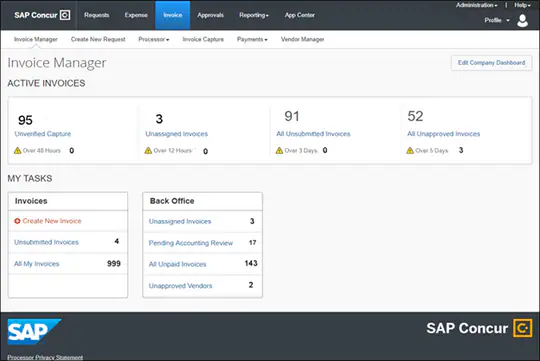
\includegraphics[width=\textwidth, height=0.4\textheight]{sap.png}

 \caption{Interface de SAP Concur}

 \label{fig:sap_concur}

 \end{figure}

 \item \textbf{Expensya} : Solution française de gestion des notes de frais, très présente sur le marché européen et nord-africain. Expensya propose une application mobile intuitive, la capture de tickets via OCR, des règles de validation personnalisables, et des tableaux de bord analytiques.

 

 \begin{figure}[H]

 \centering

 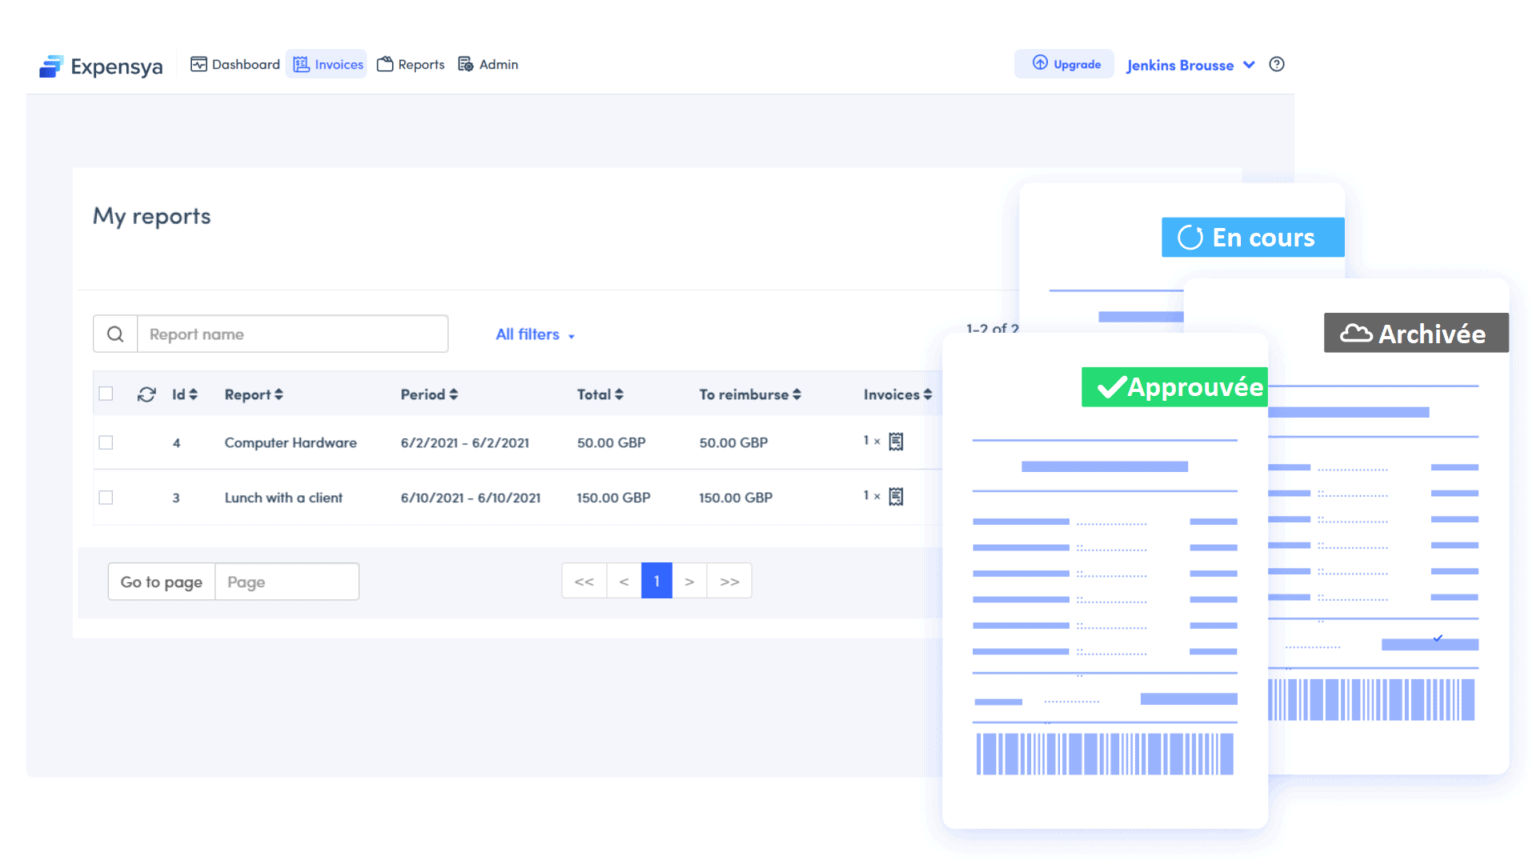
\includegraphics[width=\textwidth]{expensya1.png}

 \caption{Interface d'Expensya}

 \label{fig:expensya}

 \end{figure}

 \newpage



 \item \textbf{Rydoo} : Solution SaaS dédiée à la gestion des notes de frais et des dépenses professionnelles. Elle propose une interface moderne, une capture mobile des reçus, une reconnaissance automatique des montants et dates via OCR, ainsi qu'une intégration avec les principaux ERP (Sage, SAP, Excel). Elle cible principalement les PME, ETI et services financiers.

 

 \begin{figure}[H]

 \centering

 
\includegraphics[width=0.5\textwidth]{rydoo.png}

 \caption{Interface de Rydoo}

 \label{fig:rydoo}

 \end{figure}

\end{itemize}



\subsection{Critique de l'existant}

Les solutions actuelles présentent des forces et des faiblesses. Pour éclairer notre choix, nous les comparons selon plusieurs critères, classés ci-dessous de l’essentiel (impact direct sur la gestion des notes de frais) au plus annexe. Chaque critère est d’abord défini brièvement.



\textbf{Définition des critères :}

\begin{itemize}

 \item \textbf{Type de solution} : nature et architecture de la solution (SaaS, suite intégrée, etc.). Détermine la flexibilité, l’évolutivité et l’indépendance technologique.

 

 \item \textbf{Open source} : disponibilité du code source et possibilité de modification. Permet une adaptation complète aux besoins spécifiques de l’entreprise.

 

 \item \textbf{OCR / reconnaissance de tickets} : capacité à scanner automatiquement les justificatifs et à en extraire les informations clés (montant, date, fournisseur). Réduit la saisie manuelle, limite les erreurs et accélère le traitement.

 

 \item \textbf{Adaptation au marché tunisien} : conformité aux spécificités locales (réglementation, devises, support client en français, intégration avec les systèmes bancaires locaux). Essentiel pour garantir une adoption rapide et un fonctionnement conforme.

 

 \item \textbf{Cible principale} : type d’entreprises pour lequel la solution a été conçue (grands comptes, PME, startups). Indique l’adéquation avec la taille et les besoins de l’organisation.

 

 \item \textbf{Simplicité de déploiement} : temps et effort d’installation et de paramétrage. Un déploiement rapide évite des semaines de formation et d’arrêt des services.

 

 \item \textbf{Automatisation des processus} : circuit structuré (manager → admin → remboursement). Garantit la traçabilité, la conformité et évite les fraudes.

 

 \item \textbf{Détection d’anomalies} : repérage des doublons, dépassements, fraudes. Protège l’entreprise contre les pertes financières et les erreurs.

 

 \item \textbf{Gestion multi‑devises} : conversion automatique des devises étrangères (USD, EUR, GBP, etc.) vers la devise de référence. Indispensable pour les entreprises ayant des collaborateurs à l’international.

 

 \item \textbf{Gestion des remboursements} : automatisation du calcul et du paiement. Améliore la satisfaction des employés par des remboursements rapides.

 

 \item \textbf{Tableaux de bord analytiques} : indicateurs visuels de suivi des dépenses, graphiques d’évolution, alertes budgétaires. Aide au pilotage budgétaire et à la prise de décision.

 

 \item \textbf{Export comptable} : génération de fichiers pour logiciels comptables (Sage, SAP, Excel, CSV, API). Évite la ressaisie et les erreurs de report.

 

 \item \textbf{Coût estimé} : prix d’achat et de maintenance (licences, abonnements, frais de mise en œuvre). Un coût maîtrisé préserve la rentabilité, surtout pour une PME.

 

 \item \textbf{Délai de traitement d’une note} : temps entre la soumission de la note de frais par l’employé et son remboursement effectif. Un délai court améliore la trésorerie des employés et leur motivation.

\end{itemize}

\begin{longtable}{|c|p{3cm}|p{3cm}|p{3cm}|}

\caption{Critique comparative des solutions de gestion des notes de frais}

\label{tab:critique_existant}\\

\hline



\textbf{Critère} & \textbf{SAP Concur} & \textbf{Expensya} & \textbf{Rydoo} \\

\hline

\endfirsthead



\hline



\textbf{Critère} & \textbf{SAP Concur} & \textbf{Expensya} & \textbf{Rydoo} \\

\hline

\endhead



\hline

\multicolumn{4}{|c|}{\textit{Suite dans la page suivante}} \\

\hline

\endfoot



\hline

\endlastfoot



\textbf{Type de solution} & Suite intégrée orientée grandes entreprises, modulaire & SaaS tout‑en‑un pour PME/ETI & SaaS dédié aux notes de frais et à la gestion des dépenses \\

\hline

\textbf{Open source} & Non, solution propriétaire & Non, solution propriétaire & Non, solution propriétaire \\

\hline

\textbf{OCR / reconnaissance de tickets} & Oui, performant, lecture automatique des factures & Oui, performant, capture mobile & Oui, reconnaissance automatique des montants et dates \\

\hline

\textbf{Adaptation au marché tunisien} & Non, paramétrage complexe et absence de support local & Partielle, peut être adapté mais peu de références & Faible, solution principalement européenne, absente du marché local \\

\hline

\textbf{Cible principale} & Grandes entreprises et multinationales & PME, startups & PME, ETI et services financiers \\

\hline

\textbf{Simplicité de déploiement} & Complexe (paramétrage long, équipe projet requise) & Simple (inscription en ligne, configuration rapide) & Assez simple (interface moderne, onboarding guidé) \\

\hline

\textbf{Automatisation des processus} & Oui (workflows configurables, validation multi‑niveaux) & Oui (workflows standards, peu personnalisables) & Oui (workflows flexibles, intégration avec ERP) \\

\hline

\textbf{Détection d’anomalies} & Oui (règles métier avancées, double‑contrôle) & Partielle (règles de base sur les doublons) & Oui (vérification des justificatifs, alerte sur dépassement) \\

\hline

\textbf{Gestion multi‑devises} & Oui (automatique, taux en temps réel) & Oui (automatique) & Oui (supporte plusieurs devises, conversion intégrée) \\

\hline

\textbf{Gestion des remboursements} & Oui (intégré aux processus comptables) & Partielle (génération d’ordres de virement) & Oui (cycle complet, jusqu’au virement) \\

\hline

\textbf{Tableaux de bord analytiques} & Oui (avancés, personnalisables) & Oui (standards, indicateurs clefs) & Oui (tableaux dynamiques, exportables) \\

\hline

\textbf{Export comptable} & Oui (multi‑formats, API) & Oui (multi‑formats) & Oui (intégration avec Sage, SAP, Excel) \\

\hline

\textbf{Coût estimé} & Élevé (licences par utilisateur, frais de mise en œuvre) & Modéré (abonnement mensuel, sans engagement) & Modéré à élevé (selon les options) \\

\hline

\textbf{Délai de traitement d’une note} & Variable (selon workflow) & Réduit (quelques jours) & Court (automatisation poussée) \\

\hline

\end{longtable}



\subsection{Synthèse des limitations}

L'analyse du marché révèle plusieurs lacunes communes à l'ensemble des solutions existantes :



\begin{itemize}

 \item \textbf{Manque d'ouverture et de personnalisation} : Aucune des solutions étudiées (SAP Concur, Expensya, Rydoo) n'est open source. Cela limite la capacité des entreprises à adapter l'outil à leurs besoins spécifiques, à l'intégrer complètement avec leur système d'information existant, et à maîtriser l'évolution de la solution sans dépendre d'un éditeur.



 \item \textbf{Détection de fraude non calibrée sur les pratiques locales} : Les algorithmes de détection d'anomalies sont conçus pour des marchés matures (Europe, Amérique du Nord). Ils ne tiennent pas compte des spécificités tunisiennes : types de justificatifs locaux, fournisseurs régionaux, seuils de dépenses habituels dans le contexte national, ou encore pratiques de remboursement propres aux entreprises tunisiennes.



 \item \textbf{Absence de souveraineté des données} : Les trois solutions hébergent l'intégralité des données financières sur des serveurs en Europe ou aux États-Unis. Pour des entreprises tunisiennes soumises à la réglementation de la HAICA ou à des exigences internes de confidentialité, l'absence d'option d'hébergement local (on-premise) représente un frein majeur à l'adoption. Rydoo et Expensya ne proposent aucune option de déploiement sur infrastructure privée.



 \item \textbf{Inadéquation des cibles commerciales} : SAP Concur est conçu pour les grandes entreprises multinationales, avec un coût et une complexité qui le rendent inaccessible aux PME tunisiennes. Expensya et Rydoo ciblent principalement les PME européennes, sans offre spécifique pour le marché nord-africain. Cette dichotomie laisse un vide pour les entreprises de taille intermédiaire (ETI) et les PME ambitieuses de la région.

\end{itemize}



Ainsi, aucune solution existante n'offre à la fois :

\begin{itemize}

 \item Une ouverture et une personnalisation suffisantes (open source),

 \item Une détection de fraude réellement calibrée sur les pratiques locales tunisiennes,

 \item Une souveraineté des données avec option d'hébergement local,

 \item Une cible commerciale adaptée aux PME/ETI de la région,

 \item Un coût maîtrisé et une simplicité de déploiement.

\end{itemize}

C'est cette lacune que Coral.io Expense entend combler.



\section{Solution proposée}

Coral.io Expense est une application web de gestion des notes de frais, conçue pour répondre aux besoins spécifiques des entreprises tunisiennes. Elle automatise le cycle de vie d'une note de frais, de la soumission par l'employé jusqu'au remboursement final, en passant par un processus de validation structuré en trois niveaux (Manager → Administrateur → Remboursement).



La solution se distingue par plusieurs atouts majeurs :



\begin{itemize}

 \item \textbf{Automatisation intelligente} : L'application simplifie et accélère chaque étape du traitement des notes de frais, réduisant ainsi les délais de remboursement et la charge administrative.

 

 \item \textbf{Gestion multi-devises} : Les employés peuvent déclarer leurs dépenses en TND, EUR ou USD. La conversion automatique vers le dinar tunisien s'effectue en temps réel, sans calcul manuel.

 

 \item \textbf{Détection avancée des fraudes et anomalies} : Un module d'intelligence artificielle analyse en continu les notes de frais pour détecter les doublons, les montants suspects ou les comportements inhabituels, protégeant ainsi l'entreprise contre les erreurs et les fraudes.

 

 \item \textbf{Tableaux de bord dynamiques} : Managers et administrateurs disposent d'indicateurs clairs sur les dépenses, les budgets des projets et l'état d'avancement des notes, facilitant ainsi le pilotage financier.

 

 \item \textbf{Notifications en temps réel} : Employés, managers et administrateurs sont informés instantanément à chaque étape (soumission, validation, refus, remboursement), garantissant une parfaite traçabilité.

 

 \item \textbf{Assistant intelligent (chatbot hybride)} : Un chatbot guide les utilisateurs, répond à leurs questions sur les règles de remboursement et les aide à remplir leurs notes de frais.

 

 \item \textbf{Exports comptables} : Les données peuvent être exportées vers les logiciels comptables les plus courants, évitant ainsi toute ressaisie manuelle et les erreurs associées.

 

 

\end{itemize}



Ainsi, Coral.io Expense répond aux lacunes identifiées chez les concurrents en proposant une solution à la fois accessible, adaptée au contexte tunisien, sécurisée et dotée d'une véritable intelligence artificielle pour la détection des fraudes.



\section{Méthodologie utilisée}

Choisir une méthodologie de développement adaptée est déterminant pour la réussite d’un projet logiciel. Ce choix dépend de plusieurs facteurs : la nature du projet, la flexibilité attendue, la complexité des fonctionnalités, la taille de l’équipe et les contraintes de délais. Pour notre application Coral.io Expense, nous avons opté pour une approche agile, et plus spécifiquement pour le cadre SCRUM.





% Hide this subsection from TOC (section has only one subsection)

\addtocontents{toc}{\protect\setcounter{tocdepth}{1}}

\subsection{Pourquoi Scrum ?}

\addtocontents{toc}{\protect\setcounter{tocdepth}{2}}

Scrum n’a pas été choisi par simple effet de mode, mais parce qu’il répond précisément aux caractéristiques de notre projet :



\begin{itemize}

 \item \textbf{Un besoin métier évolutif} : La détection d’anomalies par IA, la gestion des devises ou les processus de validation n’étaient pas totalement figés au départ. Scrum permet d’ajuster les priorités à chaque sprint en fonction des retours du commanditaire et des tests utilisateurs.

 

 \item \textbf{Un livrable attendu en temps contraint} : Le stage ayant une durée limitée, Scrum impose des itérations courtes (sprints de 1 à 2 semaines) garantissant une production régulière d’incréments potentiellement livrables. Cela évite l’effet « tunnel » où rien n’est visible avant la fin.

 

 \item \textbf{Un projet à composantes multiples} : Entre le front-end Angular, les microservices Spring Boot, le service IA en Python et l’infrastructure Docker, Scrum facilite la coordination d’une petite équipe pluridisciplinaire via des rituels quotidiens (daily meeting) et un backlog unique.

 

 \item \textbf{Un feedback continu indispensable} : L’utilisateur final (manager, admin) a pu tester chaque sprint et suggérer des améliorations (ex: seuil de détection des anomalies, visibilité des justificatifs). Scrum intègre naturellement ces retours sans casser le planning.

 

 \item \textbf{Une maîtrise des risques} : Des fonctionnalités critiques ont été développées lors des premiers sprints. En cas de difficulté technique, Scrum permet de réorienter le sprint suivant sans remettre en cause l’ensemble du projet.

\end{itemize}

Ainsi, Scrum n’est pas une simple étiquette : c’est un cadre de travail qui nous a apporté visibilité, adaptabilité et efficacité tout au long du développement de Coral.io Expense.



\begin{figure}[H]

 \centering

 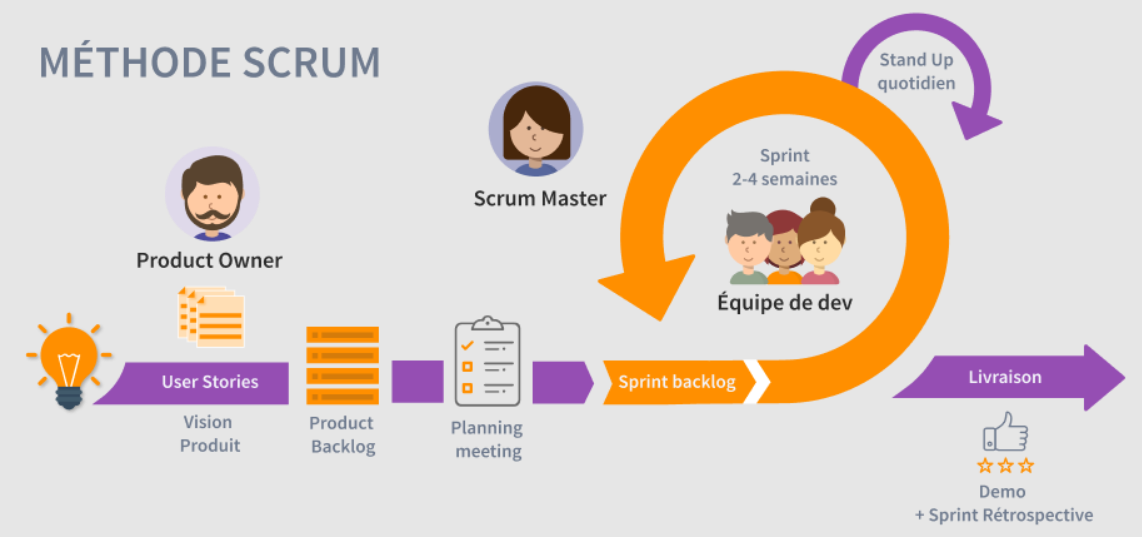
\includegraphics[width=0.8\textwidth]{scrum.png}

 \caption{Architecture Scrum}

 \label{fig:scrum}

\end{figure}

\section{Langage de modélisation UML}

Le Langage de Modélisation Unifié (UML) est un langage de modélisation graphique à base de pictogrammes conçu comme une méthode normalisée de visualisation dans les domaines du développement logiciel et en conception orientée objet.



\begin{figure}[H]

 \centering

 
\includegraphics[width=0.2\textwidth]{uml.png}

 \caption{Logo UML}

 \label{fig:logo_uml}

\end{figure}

\section{Choix technologiques adoptés}



\subsection{Environnement matériel}

Ce tableau décrit l'environnement matériel en listant les composants techniques des deux machines utilisées.



\begin{table}[H]

 \centering

 \caption{Configurations des machines}

 \label{tab:machines}

 \begin{tabular}{|p{3.5cm}|p{5cm}|p{5cm}|}

 \hline

 \textbf{Composant} & \textbf{Machine 1} & \textbf{Machine 2} \\

 \hline

 Modèle & Lenovo IdeaPad Slim 3 & MSI Thin GF63 12UCX \\

 \hline

 Processeur & Intel Core & Intel Core \\

 \hline

 RAM & 16,0 Go & 16,0 Go \\

 \hline

 Stockage & SSD & SSD \\

 \hline

 \end{tabular}

\end{table}



\subsection{Choix technologiques}



Les choix technologiques retenus pour le développement sont détaillés ci-dessous.



\subsubsection*{a) Environnements de développement}

\addcontentsline{toc}{subsubsection}{a) Environnements de développement}

\begin{itemize}

 \item \textbf{Visual Studio Code} : éditeur de code open-source de Microsoft, utilisé pour le développement rapide du front-end Angular et des scripts annexes. Sa légèreté et son riche écosystème d'extensions permettent un développement front-end efficace.

 

 \begin{figure}[H]

 \centering

 
\includegraphics[width=0.1\textwidth]{vs.jpg}

 \caption{Logo Visual Studio Code}

 \label{fig:vscode}

 \end{figure}

 

 \item \textbf{IntelliJ IDEA} : IDE Java puissant développé par JetBrains, utilisé pour le développement des microservices Spring Boot. Sa compréhension avancée du code Spring et ses outils intégrés accélèrent le développement back-end.

 

 \begin{figure}[H]

 \centering

 
\includegraphics[width=0.1\textwidth]{intellij.png}

 \caption{Logo IntelliJ IDEA}

 \label{fig:intellij}

 \end{figure}

 

 \item \textbf{PyCharm} : IDE dédié au développement du service IA de détection d'anomalies avec FastAPI. Ses fonctionnalités spécifiques à Python (débogueur, environnement virtuel) sont indispensables pour le service IA.

 

 \begin{figure}[H]

 \centering

 
\includegraphics[width=0.1\textwidth]{pycharm.png}

 \caption{Logo PyCharm}

 \label{fig:pycharm}

 \end{figure}

\end{itemize}



\subsubsection*{b) Versionnement et collaboration}

\addcontentsline{toc}{subsubsection}{b) Versionnement et collaboration}

\begin{itemize}

 \item \textbf{Git} : outil de versionnement qui permet de suivre l'évolution du code source. Le versionnement est essentiel pour gérer les évolutions concurrentes sur les différents microservices.

 

 \begin{figure}[H]

 \centering

 
\includegraphics[width=0.12\textwidth]{git.png}

 \caption{Logo Git}

 \label{fig:git}

 \end{figure}

 

 \item \textbf{GitHub} : plateforme d'hébergement de code source qui facilite la collaboration entre les membres de l'équipe. Elle centralise le code et offre les fonctionnalités de revue et de suivi des tâches.

 

 \begin{figure}[H]

 \centering

 
\includegraphics[width=0.1\textwidth]{github.png}

 \caption{Logo GitHub}

 \label{fig:github}

 \end{figure}

\end{itemize}



\subsubsection*{c) Design et maquettage}

\addcontentsline{toc}{subsubsection}{c) Design et maquettage}

\begin{itemize}

 \item \textbf{draw.io} : outil de conception de diagrammes d'architecture et de schémas de workflow. Cet outil gratuit et intégré au navigateur facilite la conception visuelle de l'architecture système.

 

 \begin{figure}[H]

 \centering

 
\includegraphics[width=0.1\textwidth]{draw.io.png}

 \caption{Logo draw.io}

 \label{fig:drawio}

 \end{figure}

 

 \item \textbf{Figma} : outil de conception d'interfaces utilisé pour réaliser les maquettes de l'application. Le maquettage préalable évite les allers-retours coûteux lors du développement front-end.

 

 \begin{figure}[H]

 \centering

 
\includegraphics[width=0.09\textwidth]{figma2.png}

 \caption{Logo Figma}

 \label{fig:figma}

 \end{figure}

\end{itemize}



\subsubsection*{d) Frameworks et langages front-end}

\addcontentsline{toc}{subsubsection}{d) Frameworks et langages front-end}

\begin{itemize}

 \item \textbf{Angular} : framework front-end qui construit l'interface web dynamique de Coral.io Expense. Angular structure le code en composants réutilisables, indispensable pour une application métier évolutive.

 

 \begin{figure}[H]

 \centering

 
\includegraphics[width=0.15\textwidth]{angular.png}

 \caption{Logo Angular}

 \label{fig:angular}

 \end{figure}

 

 \item \textbf{TypeScript} : langage qui apporte la typisation statique au code Angular pour plus de robustesse. Le typage statique détecte les erreurs à la compilation, indispensable dans une équipe de plusieurs développeurs.

 

 \begin{figure}[H]

 \centering

 
\includegraphics[width=0.1\textwidth]{ts.png}

 \caption{Logo TypeScript}

 \label{fig:typescript}

 \end{figure}

 

 \item \textbf{HTML} : langage de balisage structurant le contenu des pages web de l'application. Il sert de socle à l'interface utilisateur générée par Angular.

 

 \begin{figure}[H]

 \centering

 
\includegraphics[width=0.1\textwidth]{html.png}

 \caption{Logo HTML}

 \label{fig:html}

 \end{figure}

 

 \item \textbf{SCSS} : extension du CSS permettant d'écrire des feuilles de style plus maintenables avec des variables et du code imbriqué. Il est utilisé pour personnaliser l'apparence des composants Angular au-delà de Bootstrap.

 

 \begin{figure}[H]

 \centering

 
\includegraphics[width=0.1\textwidth]{scss.png}

 \caption{Logo SCSS}

 \label{fig:scss}

 \end{figure}

 

 \item \textbf{Bootstrap} : bibliothèque CSS accélérant la construction de l'interface utilisateur responsive. Ses composants pré-stylisés permettent de livrer une interface professionnelle sans écrire tout le CSS manuellement.

 

 \begin{figure}[H]

 \centering

 
\includegraphics[width=0.1\textwidth]{bootstrap.jpg}

 \caption{Logo Bootstrap}

 \label{fig:bootstrap}

 \end{figure}

\end{itemize}



\subsubsection*{e) Frameworks et langages back-end}

\addcontentsline{toc}{subsubsection}{e) Frameworks et langages back-end}

\begin{itemize}

 \item \textbf{Spring Boot} : framework Java qui implémente les microservices métier et l'API Gateway. Son auto-configuration et son intégration avec l'écosystème Spring simplifient la création des microservices.

 

 \begin{figure}[H]

 \centering

 
\includegraphics[width=0.12\textwidth]{sb.png}

 \caption{Logo Spring Boot}

 \label{fig:springboot}

 \end{figure}

 

 \item \textbf{Java} : langage orienté objet utilisé pour implémenter les microservices Spring Boot. Sa robustesse et son écosystème mature garantissent la fiabilité du back-end.

 

 \begin{figure}[H]

 \centering

 
\includegraphics[width=0.1\textwidth]{java.png}

 \caption{Logo Java}

 \label{fig:java}

 \end{figure}

 

 \item \textbf{Python} : langage utilisé pour écrire le service IA de détection des anomalies. La richesse de ses bibliothèques scientifiques (pandas, scikit-learn) est nécessaire pour le traitement des données financières.

 

 \begin{figure}[H]

 \centering

 
\includegraphics[width=0.1\textwidth]{python.jpg}

 \caption{Logo Python}

 \label{fig:python}

 \end{figure}

 

 \item \textbf{FastAPI} : framework Python qui expose les endpoints du service IA pour les autres microservices. Sa rapidité et sa génération automatique de documentation OpenAPI facilitent l'intégration avec les autres services.

 

 \begin{figure}[H]

 \centering

 
\includegraphics[width=0.1\textwidth]{fapi.png}

 \caption{Logo FastAPI}

 \label{fig:fastapi}

 \end{figure}

\end{itemize}



\subsubsection*{f) Base de données}

\addcontentsline{toc}{subsubsection}{f) Base de données}

\begin{itemize}

 \item \textbf{PostgreSQL} : base de données relationnelle stockant toutes les données de l'application. La fiabilité et le respect des standards SQL de PostgreSQL garantissent l'intégrité des données financières.

 

 \begin{figure}[H]

 \centering

 
\includegraphics[width=0.12\textwidth]{pgsql.png}

 \caption{Logo PostgreSQL}

 \label{fig:postgresql}

 \end{figure}

\end{itemize}



\subsubsection*{g) Sécurité}

\addcontentsline{toc}{subsubsection}{g) Sécurité}

\begin{itemize}

 \item \textbf{Keycloak} : solution de gestion d'authentification et des rôles (Employé, Manager, Administrateur). Déléguer la gestion des utilisateurs à Keycloak sécurise l'application sans réinventer la roue.

 

 \begin{figure}[H]

 \centering

 
\includegraphics[width=0.15\textwidth]{keycloak.jpg}

 \caption{Logo Keycloak}

 \label{fig:keycloak}

 \end{figure}

\end{itemize}



\subsubsection*{h) Conteneurisation}

\addcontentsline{toc}{subsubsection}{h) Conteneurisation}

\begin{itemize}

 \item \textbf{Docker} : plateforme de conteneurisation qui isole chaque microservice pour un déploiement cohérent. Les conteneurs garantissent un environnement d'exécution identique entre le développement et la production.

 

 \begin{figure}[H]

 \centering

 
\includegraphics[width=0.25\textwidth]{docker1.png}

 \caption{Logo Docker}

 \label{fig:docker}

 \end{figure}

\end{itemize}



\subsubsection*{i) Tests et documentation d'API}

\addcontentsline{toc}{subsubsection}{i) Tests et documentation d'API}

\begin{itemize}

 \item \textbf{Postman} : outil de test et de documentation d'API REST. Il permet de valider les endpoints des microservices Spring Boot et FastAPI avant l'intégration avec le front-end.

 

 \begin{figure}[H]

 \centering

 
\includegraphics[width=0.1\textwidth]{postman.png}

 \caption{Logo Postman}

 \label{fig:postman}

 \end{figure}

\end{itemize}



\newpage

\section*{Conclusion}

\addcontentsline{toc}{section}{Conclusion}

Dans ce chapitre, nous avons présenté le cadre du projet, l'entreprise d'accueil Coral-io, analysé l'existant et proposé notre solution Coral.io. Nous avons également exposé la méthodologie Scrum adoptée et les choix technologiques. Cette étude nous permet d'aborder le chapitre suivant dédié à l'analyse et la spécification des besoins.

\chapter{État de l'art}

\section*{Introduction}
\addcontentsline{toc}{section}{Introduction}

Ce chapitre présente les concepts fondamentaux et les technologies clés utilisées dans le développement de Coral.io Expense. Nous y définissons les notions d'intelligence artificielle et d'apprentissage automatique, puis nous détaillons les technologies spécifiquement mises en œuvre dans notre solution : l'OCR pour l'extraction de texte à partir de justificatifs, les LLM pour la structuration des données et la comparaison sémantique, FAISS pour la recherche de similarité vectorielle, SentenceTransformer pour les embeddings, Isolation Forest pour la détection d'anomalies, FastAPI et l'architecture microservices qui orchestrent l'ensemble, ainsi que Docker pour la conteneurisation et le déploiement. Enfin, nous présentons la méthodologie CRISP-DM qui a guidé le développement du module d'intelligence artificielle lors du sprint 4.

\section{Intelligence Artificielle}

\subsection{Définition}

L'Intelligence Artificielle (IA) est une discipline scientifique visant à créer des machines capables de reproduire certaines formes d'intelligence humaine. Elle regroupe l'apprentissage automatique (Machine Learning) et l'apprentissage profond (Deep Learning). L'IA permet d'automatiser des tâches complexes, d'analyser de grands volumes de données et de prendre des décisions adaptées.

\subsection{Apprentissage Automatique (Machine Learning)}

Le Machine Learning est un sous-domaine de l'IA qui consiste à créer des modèles capables d'apprendre à partir de données sans être explicitement programmés pour chaque tâche. Il se divise en trois grandes catégories :

\begin{itemize}
 \item \textbf{Apprentissage supervisé} : le modèle est entraîné sur des données étiquetées.
 \item \textbf{Apprentissage non supervisé} : le modèle cherche des structures dans des données non étiquetées. C'est dans cette catégorie que se situe Isolation Forest, que nous utilisons pour la détection des montants suspects.
 \item \textbf{Apprentissage par renforcement} : le modèle apprend par essais-erreurs en recevant des récompenses ou des punitions.
\end{itemize}

\subsection{Apprentissage profond (Deep Learning)}

Le Deep Learning est une technique d'apprentissage automatique basée sur des réseaux de neurones artificiels comportant plusieurs couches cachées. Il est particulièrement performant pour traiter des données non structurées comme les images, le son ou le texte. Les modèles Transformer (qui sous-tendent les LLM que nous utilisons) reposent sur cette architecture.

\section{Technologies spécifiques au projet}

\subsection{OCR (Optical Character Recognition)}

\subsubsection{Définition}

L'OCR (Reconnaissance Optique de Caractères) est une technologie permettant de convertir des images de texte (scannées, photographiées) en texte exploitable par une machine. Elle est essentielle pour traiter les justificatifs de frais (factures, accords de mission) déposés sous forme de PDF scannés ou d'images.

\subsubsection{Outils OCR utilisés dans Coral.io Expense}

\begin{itemize}
 \item \textbf{PaddleOCR} : moteur OCR léger et multilingue, performant sur les documents français, anglais et arabes. Il est notre outil principal pour les images et les PDF scannés.
 \item \textbf{Tesseract} : moteur OCR open source de Google, utilisé en solution de repli lorsque PaddleOCR ne parvient pas à fournir une extraction satisfaisante.
 \item \textbf{pdfplumber} : bibliothèque Python pour extraire le texte natif des PDF textuels (sans OCR). Très rapide et précis, elle est privilégiée pour les accords de mission au format PDF texte.
\end{itemize}

\subsection{LLM (Large Language Models)}

\subsubsection{Définition}

Un LLM (Modèle de Langage de Grande Taille) est un modèle d'IA entraîné sur des quantités massives de texte. Il est capable de comprendre et de générer du langage naturel. Dans notre projet, les LLM sont utilisés pour deux tâches principales : la structuration de textes OCRisés (extraction de montants, dates, commerçants) et la comparaison sémantique entre un accord de mission et une note de frais.

\subsubsection{Modèles évalués et modèle retenu}

\begin{itemize}
 \item \textbf{Gemma3:4b} : modèle de 4 milliards de paramètres de Google, spécialisé pour les tâches d'extraction structurée. Rapide (450 ms par requête) et précis sur les documents français. \textbf{Ce modèle a été retenu pour notre solution.}
 \item \textbf{Mistral 7B} : modèle de 7 milliards de paramètres, optimisé pour le suivi d'instructions. Bonnes performances générales mais plus lent (850 ms).
 \item \textbf{Llama 3 8B} : modèle de 8 milliards de paramètres de Meta, très performant en compréhension du langage naturel. Plus lent (1200 ms).
\end{itemize}

\subsubsection{Serveur Ollama}

Ollama est un serveur local permettant d'exécuter des LLM facilement. Il expose une API REST et gère le téléchargement, l'installation et l'exécution des modèles. Dans notre architecture, Ollama tourne sur le port 11434 et sert à la fois pour l'extraction structurée des factures et pour le chatbot hybride.

\subsection{FAISS (Facebook AI Similarity Search)}

\subsubsection{Définition}

FAISS est une bibliothèque développée par Facebook pour la recherche de similarité vectorielle à grande échelle. Elle permet d'indexer des embeddings (représentations numériques de texte) et de trouver rapidement les documents les plus proches.

\subsubsection{Application dans le projet}

FAISS est utilisé pour la détection des doublons de justificatifs. Chaque document est transformé en vecteur (embedding) via SentenceTransformer, puis indexé. Lors de l'upload d'un nouveau document, son embedding est comparé à l'index pour détecter les similarités. Le seuil de similarité a été fixé à 0,95 après optimisation.

\subsection{SentenceTransformer}

\subsubsection{Définition}

SentenceTransformer est un modèle qui transforme un texte en vecteur (embedding) de dimensions fixes (généralement 384 ou 768). La distance entre deux embeddings mesure la similarité sémantique des textes. Cette approche permet de comparer le contenu sémantique de deux documents, même si leurs formulations textuelles diffèrent.

\subsubsection{Embedding}

Un embedding est une représentation vectorielle d'un texte (mot, phrase ou document) dans un espace continu de dimensions fixes. Dans cet espace, deux textes sémantiquement proches auront des vecteurs proches, tandis que des textes de sens différent auront des vecteurs éloignés. Cette propriété permet de mesurer la similarité sémantique entre deux documents par le calcul de la distance (cosinus, euclidienne, etc.) entre leurs embeddings. Dans notre projet, les embeddings sont utilisés à la fois pour la détection des doublons (via FAISS) et pour la comparaison sémantique entre accords et notes de frais.

\subsubsection{Modèle utilisé}

Nous utilisons \texttt{all-MiniLM-L6-v2}, un modèle léger (384 dimensions) qui offre un excellent compromis entre précision (98\%) et rapidité (120 ms par fichier).

\subsection{Isolation Forest}

\subsubsection{Définition}

Isolation Forest est un algorithme non supervisé de détection d'anomalies. Il fonctionne en isolant les observations anormales qui sont plus faciles à séparer des observations normales.

\subsubsection{Application dans le projet}

Isolation Forest est utilisé pour détecter les montants suspects dans les notes de frais. Il compare un nouveau montant à l'historique des dépenses de l'employé pour une catégorie donnée. Le modèle est entraîné sur l'historique des lignes de frais remboursées.

\subsection{FastAPI et l'architecture microservices pour l'IA}

\subsubsection{Définition}

FastAPI est un framework web moderne pour la construction d'API avec Python, caractérisé par sa haute performance (grâce à Starlette et Pydantic) et sa génération automatique de documentation OpenAPI.

\subsubsection{Architecture déployée dans Coral.io Expense}

Dans notre projet, l'intelligence artificielle n'est pas intégrée directement dans le backend principal. Nous avons opté pour une architecture en microservices découplés :

\begin{itemize}
 \item \textbf{Backend Java (Spring Boot, port 8888)} : orchestration des appels aux services IA. Il reçoit les requêtes du front-end Angular et se charge d'invoquer les microservices Python appropriés.
 \item \textbf{Microservice Python unifié (FastAPI, port 9000)} : regroupe la détection de doublons (FAISS), l'analyse des factures (OCR + LLM), la détection des montants suspects (Isolation Forest) et l'extraction automatique des champs.
 \item \textbf{Microservice Python d'analyse de documents (FastAPI, port 8000)} : dédié à l'extraction structurée des accords de mission et à la comparaison sémantique avec le formulaire de note de frais.
 \item \textbf{Ollama (port 11434)} : serveur local de LLM (Gemma3:4b) pour les analyses sémantiques et le chatbot.
\end{itemize}

Ce découpage permet d'isoler la logique d'IA, de faciliter son évolution et de la scaler indépendamment du reste de l'application.

\subsection{Docker}

\subsubsection{Définition}

Docker est une plateforme open-source de conteneurisation qui permet d'empaqueter une application et ses dépendances dans un conteneur isolé, garantissant ainsi un environnement d'exécution identique quel que soit l'hôte (développement, test, production).

\subsubsection{Avantages de Docker}

\begin{itemize}
 \item \textbf{Reproductibilité} : un conteneur exécute le même code et les mêmes dépendances sur toutes les machines.
 \item \textbf{Isolation} : chaque microservice tourne dans son propre conteneur, évitant les conflits de versions.
 \item \textbf{Légèreté} : les conteneurs partagent le noyau de l'hôte, contrairement aux machines virtuelles.
 \item \textbf{Déploiement simplifié} : une seule commande (\texttt{docker-compose up -d}) lance l'ensemble des services.
\end{itemize}

\subsubsection{Application dans Coral.io Expense}

Dans notre projet, Docker a été utilisé pour conteneuriser l'ensemble des composants :

\begin{itemize}
 \item \textbf{Base de données PostgreSQL} : conteneur isolé pour les données de l'application.
 \item \textbf{Keycloak} : serveur d'authentification conteneurisé.
 \item \textbf{Backend Spring Boot (port 8888)} : microservice métier Java.
 \item \textbf{Microservice Python FastAPI (port 9000)} : détection de doublons, analyse de factures, montants suspects.
 \item \textbf{Microservice Python FastAPI (port 8000)} : analyse des accords de mission.
 \item \textbf{Ollama (port 11434)} : serveur de LLM pour les analyses sémantiques.
\end{itemize}

L'orchestration est assurée par Docker Compose, qui définit dans un fichier \texttt{docker-compose.yml} l'ensemble des services, leurs ports, leurs volumes et leurs dépendances. Cette approche a permis de :
\begin{itemize}
 \item Uniformiser l'environnement de développement entre les deux membres de l'équipe.
 \item Tester l'intégration complète avant le déploiement final.
 \item Faciliter la mise en production chez un client potentiel.
\end{itemize}

\section{Méthodologie de gestion de projet Data Science : CRISP-DM}

\subsection{Présentation des méthodologies existantes}

Plusieurs méthodologies existent pour la gestion de projets data science :

\begin{itemize}
 \item \textbf{KDD (Knowledge Discovery in Databases)} : processus en cinq étapes (sélection, préparation, exploration, modélisation, évaluation) centré sur l'extraction de connaissances à partir de données.
 \item \textbf{SEMMA (Sample, Explore, Modify, Model, Assess)} : développé par SAS, il couvre les phases techniques du data mining mais occulte les phases de compréhension du métier et de déploiement.
 \item \textbf{CRISP-DM (Cross-Industry Standard Process for Data Mining)} : méthodologie de référence en six phases itératives, indépendante des outils et intégrant une phase de déploiement rigoureuse.
\end{itemize}

\subsection{Application de CRISP-DM dans Coral.io Expense}

Pour le développement des composants d'intelligence artificielle (regroupés dans le Sprint 4), nous avons appliqué la méthodologie CRISP-DM. Ce choix a été motivé par plusieurs facteurs :

\begin{itemize}
 \item La détection des anomalies dans les notes de frais ne se limite pas à l'implémentation d'un modèle : elle nécessite une approche structurée couvrant l'ensemble du cycle de vie des données.
 \item CRISP-DM est indépendant de tout outil ou technologie, ce qui permet de l'adapter à notre architecture microservices.
 \item Ses phases itératives correspondent parfaitement au besoin d'amélioration continue des modèles.
 \item Contrairement à SEMMA, CRISP-DM intègre une phase de déploiement qui nous a permis de mettre en production les modèles FAISS et Isolation Forest.
\end{itemize}

Les six phases de CRISP-DM telles qu'appliquées dans notre projet sont :

\begin{enumerate}
 \item \textbf{Compréhension du métier} : définition des objectifs (détection des doublons, des montants suspects, cohérence accord/note).
 \item \textbf{Compréhension des données} : analyse d'un échantillon de 300 notes de frais pour identifier les types d'anomalies.
 \item \textbf{Préparation des données} : nettoyage OCR, normalisation des dates et montants, indexation FAISS, extraction structurée des accords.
 \item \textbf{Modélisation} : tests comparatifs de trois approches pour les doublons (hash MD5, BERT, FAISS) et trois LLM pour l'extraction (Mistral, Gemma, Llama).
 \item \textbf{Évaluation} : validation des modèles sur jeu de test avec calcul des métriques (précision, rappel, F1-score).
 \item \textbf{Déploiement} : sauvegarde des modèles, conteneurisation des microservices FastAPI, intégration dans l'interface web.
\end{enumerate}

\section{L'apprentissage par transfert (Transfer Learning)}

L'apprentissage par transfert consiste à transférer des connaissances acquises lors de l'apprentissage d'une tâche vers une autre tâche similaire. Dans notre projet, nous utilisons cette approche à plusieurs niveaux :

\begin{itemize}
 \item \textbf{SentenceTransformer all-MiniLM-L6-v2} : modèle pré-entraîné sur un corpus large, utilisé sans fine-tuning pour les embeddings de détection de doublons.
 \item \textbf{LLM Gemma3:4b} : modèle pré-entraîné par Google, utilisé pour l'extraction structurée et le chatbot.
 \item \textbf{Isolation Forest} : algorithme non supervisé entraîné spécifiquement sur l'historique des dépenses de l'application.
\end{itemize}

\section{Conclusion}

Ce chapitre a présenté les concepts fondamentaux et les technologies spécifiquement utilisées dans le développement de Coral.io Expense. Les notions d'IA, de Machine Learning et de Deep Learning ont été définies. Les technologies mises en œuvre ont été détaillées : OCR (PaddleOCR, Tesseract, pdfplumber), LLM (Gemma3:4b via Ollama), FAISS pour la recherche de similarité, SentenceTransformer pour les embeddings, Isolation Forest pour la détection d'anomalies, FastAPI pour l'architecture microservices dédiée à l'IA, et Docker pour la conteneurisation et le déploiement de l'ensemble des services. Enfin, la méthodologie CRISP-DM a été présentée comme le cadre de travail pour le développement du module d'intelligence artificielle du sprint 4. Ces bases théoriques permettent d'aborder sereinement les chapitres de réalisation.

% ============================================================

% CHAPITRE 2 : ANALYSE ET SPÉCIFICATION DES BESOINS

% ============================================================

\chapter{Analyse et spécification des besoins}



\section*{Introduction}

\addcontentsline{toc}{section}{Introduction}

Dans ce chapitre, nous présentons les besoins du projet d'application de gestion de notes de frais Coral.io. Nous identifierons les différentes parties prenantes, définirons les besoins fonctionnels et non fonctionnels, en mettant un accent particulier sur les fonctionnalités d'intelligence artificielle, de conversion de devises et d'expérience utilisateur avancée.



\section{Spécification des besoins}



\subsection{Identification des acteurs}

L'application Coral.io implique trois acteurs principaux :



\begin{itemize}

\item \textbf{Employé} : Demandeur de remboursement. Peut créer, soumettre et suivre ses notes de frais, bénéficier de la conversion automatique des devises et de l'assistant chatbot.



\item \textbf{Manager} : Supervise les dépenses de son département. Consulte les notes, visualise les anomalies détectées par l'IA, valide ou refuse avec commentaire.



\item \textbf{Administrateur} : Garant de la conformité. Gère les utilisateurs, les paramètres (départements, projets, catégories, taux de change), contrôle les notes, procède aux remboursements (total/partiel) et génère les ordres de paiement.

\end{itemize}

\subsection{Besoins Fonctionnels}

L'application doit répondre aux exigences suivantes :



\begin{itemize}

 \item Gestion des comptes utilisateurs : Authentification, création par admin, gestion des profils

 \item Gestion des départements : Création, modification, assignation de managers

 \item Gestion des projets : Création, association à un département, budget

 \item Gestion des catégories de dépenses : Création, plafonds

 \item Gestion des notes de frais : CRUD, soumission, workflow

 \item Gestion multi-devises : TND, EUR, USD avec conversion automatique

 \item Workflow de validation : Manager → Admin → Remboursement

 \item Gestion des remboursements : Remboursement total ou partiel

 \item Système de notifications : Email et in-app via microservice

 

 \item Détection automatique d'anomalies : Doublons et anomalies liées aux justificatifs (visible par manager et admin)

 \item Chatbot hybride : Assistant intelligent avec classification d'intents

 \item Tableaux de bord : Visualisations analytiques

 \item Export des données : Excel/CSV

\end{itemize}



\subsection{Besoins Non Fonctionnels}



\begin{table}[H]

 \centering

 \caption{Besoins non fonctionnels}

 \label{tab:non_fonctionnel}

 \begin{tabular}{|p{3.5cm}|p{10cm}|}

 \hline

 \textbf{Catégorie} & \textbf{Exigences} \\

 \hline

 Performance & - Temps de réponse < 2 secondes pour 95\% des requêtes \\

 & - Support de 100 utilisateurs simultanés \\

 & - Chargement des pages < 3 secondes \\

 \hline

 Sécurité & - Authentification JWT \\

 & - Traçabilité complète des actions \\

 & - Gestion des rôles et permissions \\

 \hline

 Disponibilité & - Disponibilité de 99,5\% \\

 & - Sauvegarde quotidienne des bases de données \\

 & - Redémarrage automatique des services \\

 \hline

 Compatibilité & - Navigateurs : Chrome, Firefox, Edge, Safari \\

 & - Formats supportés : JPEG, JPG, SVG, PNG, PDF \\

 & - Taille maximale des fichiers : 10 Mo \\

 \hline

 Extensibilité & - Architecture microservices découplés \\

 & - Ajout dynamique de champs personnalisés \\

 \hline

 Scalabilité & - Passage de 50 à 500 utilisateurs sans réarchitecture \\

 & - Montée en charge horizontale des microservices \\

 & - Mise en cache des données fréquentes \\

 \hline

 Précision IA & - Taux de détection anomalies > 85\% \\

 & - Taux de faux positifs < 10\% \\

 & - Temps d'analyse d'une note < 10 secondes \\

 \hline

 Maintenabilité & - Code documenté et commenté \\

 & - Tests unitaires (couverture > 70\%) \\

 & - Déploiement automatisé via Docker \\

 \hline

 Utilisabilité & - Interface intuitive et responsive \\

 & - Apprentissage < 15 minutes \\

 & - Messages d'erreur clairs \\

 \hline

 \end{tabular}

\end{table}

\newpage

\section{Product Backlog}

\subsection{Backlog de Produit}

\captionof{table}{Backlog de produit}

\label{tab:backlog}

\begin{longtable}{|p{2cm}|p{1cm}|p{8.3cm}|c|c|}

\hline

\textbf{Fonctionn-\newline}\textbf{alité} & \textbf{ID} & \textbf{\centering User Story} & \textbf{Estimation} & \textbf{Priorité} \\

\hline

\endfirsthead



\hline

\textbf{Fonctionn-\newline}\textbf{alité} & \textbf{ID} & \textbf{User Story} & \textbf{Estimation} & \textbf{Priorité} \\

\hline

\endhead



\hline

\multicolumn{5}{|c|}{\textit{Suite dans la page suivante}} \\

\hline

\endfoot



\hline

\endlastfoot



\multirow{10}{*}{Comptes} & 1 & En tant qu'administrateur, je veux créer un compte utilisateur afin de permettre à un nouvel employé d'accéder à la plateforme. & 2 & élevée \\

\cline{2-5}

& 2 & En tant qu'administrateur, je veux consulter la liste des comptes utilisateurs afin de visualiser rapidement les profils. & 2 & élevée \\

\cline{2-5}

& 3 & En tant qu'administrateur, je veux modifier les informations d’un compte utilisateur (rôle, département, email) afin de maintenir les données à jour. & 2 & élevée \\

\cline{2-5}

& 4 & En tant qu'administrateur, je veux activer ou désactiver un compte utilisateur afin de contrôler l’accès à la plateforme. & 2 & élevée \\

\cline{2-5}

& 5 & En tant qu'administrateur, je veux filtrer les comptes afin de trouver rapidement un profil spécifique. & 2 & moyenne \\

\cline{2-5}

& 6 & En tant qu'utilisateur, je veux m'authentifier avec mon email et mot de passe afin d'accéder à mon compte. & 3 & élevée \\

\cline{2-5}

& 7 & En tant qu'utilisateur, je veux changer mon mot de passe lors de ma première connexion afin de sécuriser mon compte et respecter les politiques de sécurité. & 3 & élevée \\

\cline{2-5}

& 8 & En tant qu'utilisateur, je veux récupérer mon mot de passe en cas d'oubli afin de ne pas bloquer mon accès à la plateforme. & 3 & moyenne \\

\cline{2-5}

& 9 & En tant qu'utilisateur, je veux consulter et modifier mon profil utilisateur afin de maintenir mes informations personnelles à jour. & 5 & élevée \\

\cline{2-5}

& 10 & En tant qu'utilisateur, je veux me déconnecter de la plateforme afin de sécuriser ma session. & 2 & élevée \\

\hline



\multirow{6}{*}\newline \newline {\parbox{2.8cm}{ Départem-\\ents}} & 11 & En tant qu'administrateur, je veux créer un département afin d'organiser la structure de l'entreprise. & 2 & élevée \\

\cline{2-5}

& 12 & En tant qu'administrateur, je veux consulter la liste des départements avec filtres afin de visualiser l'organisation. & 2 & élevée \\

\cline{2-5}

& 13 & En tant qu'administrateur, je veux modifier les informations d’un département afin de les tenir à jour. & 2 & élevée \\

\cline{2-5}

& 14 & En tant qu'administrateur, je veux supprimer un département afin de nettoyer l’annuaire. & 2 & moyenne \\

\cline{2-5}

& 15 & En tant qu'administrateur, je veux filtrer les départements afin de gérer leur visibilité. & 2 & moyenne \\

\cline{2-5}

& 16 & En tant qu'administrateur, je veux activer ou désactiver un département afin d’en suspendre temporairement l’utilisation. & 2 & élevée \\

\hline



\multirow{8}{*}{\parbox{2.8cm}{ Projets et\\règles de\\rembour-\\sement}} & 17 & En tant qu'administrateur, je veux créer un projet afin de l’associer aux notes de frais. & 2 & élevée \\

\cline{2-5}

& 18 & En tant qu'administrateur, je veux consulter la liste des projets avec filtres afin d’avoir une vision globale. & 2 & élevée \\

\cline{2-5}

& 19 & En tant qu'administrateur, je veux modifier un projet afin de mettre à jour ses informations. & 2 & élevée \\

\cline{2-5}

& 20 & En tant qu'administrateur, je veux clôturer un projet afin d’empêcher de nouvelles notes de frais dessus. & 2 & élevée \\

\cline{2-5}

& 21 & En tant qu'administrateur, je veux activer ou désactiver un projet afin de mettre à jour la possibilité de soumettre des notes. & 2 & moyenne \\

\cline{2-5}

& 22 & En tant qu'administrateur, je veux supprimer un projet définitivement afin de nettoyer la liste des projets obsolètes. & 2 & moyenne \\

\cline{2-5}

& 23 & En tant qu'administrateur, je veux affecter un employé à un projet afin de lui permettre de soumettre des notes de frais sur ce projet. & 2 & élevée \\

\cline{2-5}

& 24 & En tant qu'utilisateur, je veux consulter mes projets et les règles de remboursement afin de savoir quelle note est éligible. & 5 & moyenne \\

\hline



\multirow{7}{*}{Catégories} & 25 & En tant qu'administrateur, je veux créer une catégorie de dépense afin de définir les types de frais remboursables. & 3 & élevée \\

\cline{2-5}

& 26 & En tant qu'administrateur, je veux consulter la liste des catégories avec leurs plafonds et champs afin de vérifier leur configuration. & 2 & élevée \\

\cline{2-5}

& 27 & En tant qu'administrateur, je veux modifier une catégorie afin d’adapter les règles de remboursement. & 2 & élevée \\

\cline{2-5}

& 28 & En tant qu'administrateur, je veux supprimer une catégorie afin de nettoyer la configuration. & 2 & moyenne \\

\cline{2-5}

& 29 & En tant qu'administrateur, je veux activer ou désactiver une catégorie afin de la rendre temporairement indisponible. & 2 & élevée \\

\cline{2-5}

& 30 & En tant qu'administrateur, je veux ajouter des champs personnalisés dynamiques à une catégorie afin de collecter des informations spécifiques selon le type de dépense. & 8 & élevée \\

\cline{2-5}

& 31 & En tant qu'administrateur, je veux réutiliser un champ existant d'une catégorie à une autre afin d'éviter la duplication et d'harmoniser les données. & 5 & moyenne \\

\hline



\multirow{18}{*}\newline \newline {\parbox{2.8cm}{ Notes de \\frais}} & 32 & En tant qu'employé, je veux créer une note de frais afin de soumettre mes dépenses professionnelles au remboursement. & 8 & élevée \\

\cline{2-5}

& 33 & En tant qu'utilisateur, je veux sélectionner une devise (TND/EUR/USD) afin de déclarer ou visualiser des frais dans différentes monnaies. & 5 & élevée \\

\cline{2-5}

& 34 & En tant qu'employé, je veux consulter ma liste de notes avec filtres et pagination afin de retrouver facilement une note passée. & 5 & élevée \\

\cline{2-5}

& 35 & En tant qu'employé, je veux modifier ou supprimer une note en attente afin de corriger des erreurs avant soumission. & 5 & élevée \\

\cline{2-5}

& 36 & En tant qu'employé, je veux recevoir des notifications in-app et par email lorsque ma note est validée ou refusée par le manager afin de suivre son état. & 3 & élevée \\

\cline{2-5}

& 37 & En tant que manager, je veux lister et filtrer les notes afin d'analyser efficacement les notes de mon département. & 5 & élevée \\

\cline{2-5}

& 38 & En tant que manager, je veux recevoir des notifications in-app et par email lorsqu'une nouvelle note est soumise dans un projet de mon département afin de la traiter rapidement. & 3 & élevée \\

\cline{2-5}

& 39 & En tant qu'administrateur, je veux recevoir des notifications in-app et par email lorsqu'une note est validée par le manager avec son commentaire afin de procéder au remboursement. & 3 & élevée \\

\cline{2-5}

& 40 & En tant que manager, je veux valider une note (avec commentaire optionnel) afin de l’approuver pour remboursement. & 3 & élevée \\

\cline{2-5}

& 41 & En tant que manager, je veux refuser une note (avec commentaire obligatoire) afin de la rejeter et informer l’employé. & 3 & élevée \\

\cline{2-5}

& 42 & En tant que manager, je veux visualiser, avant de valider une note de frais, l'impact budgétaire prévisionnel sur le projet afin d'éviter de dépasser le budget alloué et de prendre une décision éclairée. & 3 & élevée \\

\cline{2-5}

& 43 & En tant que manager, je veux consulter, pour un employé sélectionné, la consommation détaillée par projet afin de surveiller que chaque membre de mon équipe ne dépasse pas sa part implicite du budget alloué aux projets. & 5 & élevée \\

\cline{2-5}

& 44 & En tant qu'utilisateur, je veux consulter l'historique complet de mes notifications (lues et non lues) avec pagination et filtres, afin de retrouver facilement une notification passée. & 3 & moyenne \\

\cline{2-5}

& 45 & En tant qu'utilisateur, je veux supprimer définitivement une notification de mon historique, afin de nettoyer ma liste et de ne conserver que les notifications pertinentes. & 2 & moyenne \\

\cline{2-5}

& 46 & En tant qu'utilisateur, je veux qu’un clic sur une notification me redirige vers la note de frais concernée, afin d’accéder rapidement à l’information sans recherche supplémentaire. & 3 & élevée \\

\cline{2-5}

& 47 & En tant qu'administrateur et manager, je veux recevoir une notification (in-app et email) lorsqu'une note soumise dépasse le plafond de sa catégorie de dépense ou entraîne un dépassement du budget alloué au projet, afin d'être alerté rapidement et de demander des justificatifs complémentaires. & 3 & élevée \\

\cline{2-5}

& 48 & En tant qu'administrateur et manager, je veux visualiser clairement les dépassements de montant (plafond de catégorie, budget projet) sur les notes de frais afin d'identifier rapidement les notes présentant des écarts anormaux et de prendre des décisions éclairées. & 2 & élevée \\

\hline



\multirow{15}{*}\newline \newline {\parbox{2.5cm}{ Rembour-\\sements}} & 49 & En tant qu'employé et manager, je veux être alerté (in-app et email) de tout événement critique sur les notes de frais (validation, refus, remboursement, rejet, soumission, ajout de note interne) afin de suivre l’évolution des demandes et de réagir rapidement. & 4 & élevée \\

\cline{2-5}

& 50 & En tant qu'administrateur et manager, je veux ajouter une note interne confidentielle à une note de frais, visible uniquement par l'autre partie, afin de communiquer des informations sensibles sans les exposer à l'employé. & 3 & moyenne \\

\cline{2-5}

& 51 & En tant qu'administrateur, je veux consulter toutes les notes validées par le manager afin de procéder à leur remboursement. & 5 & élevée \\

\cline{2-5}

& 52 & En tant qu'administrateur, je veux rembourser une note (total ou partiel) afin d'indemniser l'employé pour les frais légitimes. & 5 & élevée \\

\cline{2-5}

& 53 & En tant qu'administrateur, je veux rejeter le remboursement d'une note avec un commentaire afin d'informer l'employé et le manager de la raison du refus. & 3 & élevée \\

\cline{2-5}

& 54 & En tant qu'administrateur, je veux consulter l'ordre de paiement généré automatiquement par le système après validation d'une note de frais, afin de disposer d'un justificatif traçable et de consulter l'ordre généré. & 5 & élevée \\

\cline{2-5}

& 55 & En tant qu'administrateur, je veux consulter les ordres de paiement en attente afin de suivre les paiements à effectuer. & 3 & élevée \\

\cline{2-5}

& 56 & En tant qu'administrateur, je veux confirmer le paiement et archiver la note afin de clôturer définitivement le remboursement. & 5 & élevée \\

\cline{2-5}

& 57 & En tant qu'administrateur, je veux consulter l'archive des notes traitées afin de pouvoir retrouver un justificatif en cas d'audit. & 3 & élevée \\

\cline{2-5}

& 58 & En tant qu'administrateur, je veux visualiser, avant de confirmer un remboursement, le budget restant du projet et une alerte si le montant à rembourser dépasse ce budget, afin d'éviter de dépasser les enveloppes budgétaires. & 3 & élevée \\

\cline{2-5}

& 59 & En tant qu'administrateur, je veux consulter un tableau de bord dédié au suivi des budgets et consommations des projets, afin d'avoir une vision globale de l'état financier des projets. & 3 & élevée \\

\cline{2-5}

& 60 & En tant qu'administrateur, je veux filtrer les données du tableau de bord projets afin d'analyser la répartition des coûts et de détecter rapidement les dépassements. & 1 & élevée \\

\cline{2-5}

& 61 & En tant qu'administrateur, je veux exporter les données du tableau de bord projets afin de réaliser des reporting hors ligne ou des analyses externes. & 1 & élevée \\

\cline{2-5}

& 62 & En tant qu'administrateur, je veux exporter les notes vers Excel afin d'effectuer des analyses externes ou des reporting hors ligne. & 3 & moyenne \\

\hline



Déploiement & 63 & En tant que DevOps, je veux dockeriser l'application afin de faciliter le déploiement et l'environnement de test. & 8 & élevée \\

\hline



\multirow{5}{*}{Anomalies} & 64 & En tant qu'administrateur et manager, je veux que le système détecte automatiquement les doublons de justificatifs (factures et accords) lors de l'upload afin d'éviter les soumissions frauduleuses ou en erreur. & 5 & élevée \\

\cline{2-5}

& 65 & En tant qu'administrateur et manager, je veux que le système analyse les montants des dépenses par catégorie et par utilisateur afin de détecter les montants anormalement élevés et de signaler les anomalies potentielles. & 4 & élevée \\

\cline{2-5}

& 66 & En tant qu'administrateur et manager, je veux que le système analyse les factures afin de détecter les anomalies ou falsifications sur les justificatifs. & 4 & élevée \\

\cline{2-5}

& 67 & En tant qu'administrateur et manager, je veux que le système compare automatiquement les données du formulaire de note de frais avec l'accord de mission associé (dates, lieu, objectif, etc.) afin de détecter les anomalies sémantiques et contextuelles. & 8 & élevée \\

\cline{2-5}

& 68 & En tant qu'employé, je veux que le système remplisse automatiquement les champs du formulaire (montant, date, description, etc.) à partir de la facture téléchargée, afin de gagner du temps et de réduire les erreurs de saisie. & 8 & moyenne \\

\hline



\multirow{3}{*}{Dashboard} & 69 & En tant qu'employé, je veux visualiser des statistiques personnalisées sur mes propres notes afin de suivre l'évolution de mes dépenses. & 5 & moyenne \\

\cline{2-5}

& 70 & En tant que manager, je veux disposer d'un tableau de bord complet avec des statistiques synthétiques sur les dépenses de mon département, l'état d'avancement des notes et les alertes budgétaires. & 8 & élevée \\

\cline{2-5}

& 71 & En tant qu'administrateur, je veux consulter un tableau de bord global avec des indicateurs clés (nombre total de notes, montants remboursés par mois, anomalies détectées, délais de traitement) afin de piloter la performance financière. & 8 & élevée \\

\hline



Chatbot & 72 & En tant qu'utilisateur, je veux poser des questions au chatbot hybride afin d'obtenir une aide instantanée sur les règles de remboursement ou l'état de mes notes. & 8 & moyenne \\

\hline



\end{longtable}







\subsection{Planification des Sprints}



\begin{table}[H]

 \centering

 \caption{Planification des Sprints}

 \label{tab:sprints}

 \begin{tabular}{|p{2.2cm}|p{5cm}|p{4.8cm}|p{1.2cm}|p{1.2cm}|}

 \hline

 \textbf{ID Sprint} & \textbf{Nom du Sprint} & \textbf{User Stories} & \textbf{Date Début} & \textbf{Date Fin} \\

 \hline

 Sprint 1 & \textbf{Initialisation et socle technique} & US-1 à US-31 (Comptes, Départements, Projets, Catégories) & 10/02 & 02/03 \\

 \hline

 Sprint 2 & \textbf{Création et gestion des notes de frais} & US-32 à US-48 (Notes de frais, devises, notifications employé/manager, visualisation dépassements manager, impact budgétaire prévisionnel, consommation employé, historiques notifications) & 03/03 & 30/03 \\

 \hline

 Sprint 3 & \textbf{Remboursement, notes internes et déploiement} & US-49 à US-63 (Alertes événements critiques, notes internes, remboursements, ordres de paiement, visualisation dépassements admin, budget restant avant remboursement, dashboard projets admin, filtres, export, export Excel, déploiement Docker) & 31/03 & 27/04 \\

 \hline

 Sprint 4 & \textbf{Détection des anomalies et dashboards} & US-64 à US-72 (Détection des doublons, montants suspects, anomalies justificatifs, incohérences accord/form, remplissage automatique des factures, dashboards employé/manager/admin, chatbot) & 28/04 & 30/05 \\

 \hline

 \end{tabular}

\end{table}

\newpage

\subsection{Critères d’acceptation des User Stories prioritaires}

\addcontentsline{toc}{section}{Critères d’acceptation}

\captionof{table}{Critères d’acceptation des User Stories prioritaires}

\label{tab:Critères}

\begin{longtable}{|p{2.5cm}|p{1cm}|p{2cm}|p{8cm}|}

\hline

\textbf{Fonctionnalité} & \textbf{ID} & \textbf{Estimation} & \textbf{Critères d’acceptation} \\

\hline

\endfirsthead



\hline

\textbf{Fonctionnalité} & \textbf{ID} & \textbf{Estimation} & \textbf{Critères d’acceptation} \\

\hline

\endhead



\hline

\multicolumn{4}{|c|}{\textit{Suite dans la page suivante}} \\

\hline

\endfoot



\hline

\endlastfoot



\multirow{5}{*}{Comptes} & US-1 & 2 & \begin{itemize}

 \item L’administrateur remplit un formulaire (email, rôle, département) et valide.

 \item Le compte est créé dans Keycloak avec un mot de passe temporaire envoyé par email.

 \item L’utilisateur doit changer son mot de passe à la première connexion.

 \item Si l’email existe déjà → message d’erreur.

\end{itemize} \\

\cline{2-4}

& US-2 & 2 & \begin{itemize}

 \item L’administrateur accède à une page listant tous les utilisateurs avec pagination.

 \item Les colonnes affichées : ID, nom, email, rôle, département, statut.

 \item Possibilité de filtrer par rôle et par statut.

\end{itemize} \\

\cline{2-4}

& US-3 & 2 & \begin{itemize}

 \item L’administrateur peut modifier le rôle, le département ou l’email d’un utilisateur.

 \item Les modifications sont immédiatement effectives.



\end{itemize} \\

\cline{2-4}

& US-4 & 2 & \begin{itemize}

 \item L’administrateur peut activer ou désactiver un compte en un clic.

 \item Un compte désactivé ne peut plus se connecter.



\end{itemize} \\

\cline{2-4}

& US-6 & 3 & \begin{itemize}

 \item L’utilisateur saisit email et mot de passe.

 \item Si authentification réussie → redirection vers son tableau de bord.

 \item Si identifiants incorrects → message d’erreur.

 \item Après 5 tentatives échouées → compte temporairement bloqué.

\end{itemize} \\

\hline



\multirow{5}{*}{Départements} & US-11 & 2 & \begin{itemize}

 \item L’administrateur peut créer un département avec nom, code et description.

 \item Le code doit être unique.

 \item Le département est créé avec le statut ACTIF par défaut.

\end{itemize} \\

\cline{2-4}

& US-12 & 2 & \begin{itemize}

 \item L’administrateur voit la liste de tous les départements.

 \item Possibilité de filtrer par statut (ACTIF/INACTIF).

 \item Les colonnes : nom, code, statut, description.

\end{itemize} \\

\cline{2-4}

& US-16 & 2 & \begin{itemize}

 \item L’administrateur peut basculer un département entre ACTIF et INACTIF.

 \item Un département INACTIF n’apparaît plus dans les sélecteurs pour les employés.

 \item Les projets du département désactivé ne peuvent plus recevoir de nouvelles notes.

\end{itemize} \\

\hline



\multirow{5}{*}{Projets} & US-17 & 2 & \begin{itemize}

 \item L’administrateur crée un projet avec nom, code, budget, département.

 \item Le code doit être unique.

 \item Le projet est créé avec le statut ACTIF par défaut.

\end{itemize} \\

\cline{2-4}

& US-18 & 2 & \begin{itemize}

 \item L’administrateur visualise tous les projets avec filtres (statut, département).

 \item Les colonnes : nom, code, département, budget, statut.

\end{itemize} \\

\cline{2-4}

& US-20 & 2 & \begin{itemize}

 \item L’administrateur peut clôturer un projet.

 \item Un projet clôturé n’accepte plus de nouvelles notes de frais.

 \item Les notes existantes restent consultables.

\end{itemize} \\

\cline{2-4}

& US-23 & 2 & \begin{itemize}

 \item L’administrateur peut affecter un employé à un projet.

 \item L’employé ne peut soumettre des notes que sur les projets qui lui sont affectés.

 \item Un employé peut être affecté à plusieurs projets.

\end{itemize} \\

\hline



\multirow{5}{*}{Catégories} & US-25 & 3 & \begin{itemize}

 \item L’administrateur crée une catégorie avec nom, plafond, description.

 \item La catégorie est active par défaut.

 \item Une fois créée, elle apparaît dans le formulaire de note de frais.

\end{itemize} \\

\cline{2-4}

& US-26 & 2 & \begin{itemize}

 \item L’administrateur voit la liste des catégories avec plafonds, statut et champs dynamiques.

 \item Possibilité de filtrer par statut (actif/inactif).

\end{itemize} \\

\cline{2-4}

& US-29 & 2 & \begin{itemize}

 \item L’administrateur peut activer ou désactiver une catégorie.

 \item Une catégorie désactivée n’apparaît plus dans le formulaire de création de note.

 \item Les lignes existantes utilisant cette catégorie restent inchangées.

\end{itemize} \\

\cline{2-4}

& US-30 & 8 & \begin{itemize}

 \item L’administrateur peut ajouter des champs personnalisés (TEXT, NUMBER, DATE, SELECT).

 \item Les champs sont affichés dynamiquement dans le formulaire.

 \item Les valeurs saisies sont correctement sauvegardées en base.

 \item Un champ SELECT affiche les options configurées.

\end{itemize} \\

\hline



\multirow{5}{*}{Notes de frais} & US-32 & 8 & \begin{itemize}

 \item L’employé remplit un formulaire multi-étapes : projet, lignes de frais, accord.

 \item Les champs dynamiques s’adaptent à la catégorie sélectionnée.

 \item La note est enregistrée avec le statut EN\_ATTENTE.

 \item Les justificatifs et l’accord sont correctement stockés.

\end{itemize} \\

\cline{2-4}

& US-33 & 5 & \begin{itemize}

 \item L’utilisateur sélectionne une devise (TND/EUR/USD) dans le menu profil.

 \item Tous les montants affichés sont convertis dans la devise choisie.

 \item La préférence est sauvegardée pour les connexions futures.

\end{itemize} \\

\cline{2-4}

& US-34 & 5 & \begin{itemize}

 \item L’employé voit ses notes dans un tableau paginé avec filtres (statut, projet, période).

 \item Un clic sur « Détails » ouvre la popup de visualisation.

 \item Les notes EN\_ATTENTE ont des boutons « Modifier » et « Supprimer ».

\end{itemize} \\

\cline{2-4}

& US-35 & 5 & \begin{itemize}

 \item L’employé peut modifier une note EN\_ATTENTE.

 \item Une note modifiée conserve son statut EN\_ATTENTE.

 \item L’employé peut supprimer une note EN\_ATTENTE avec confirmation.

\end{itemize} \\

\cline{2-4}

& US-36 & 3 & \begin{itemize}

 \item L’employé reçoit une notification in-app et un email quand sa note est validée ou refusée.

 \item La notification contient le numéro de note et le commentaire du manager (pour un refus).

\end{itemize} \\

\cline{2-4}

& US-37 & 5 & \begin{itemize}

 \item Le manager voit les notes de son département avec filtres (statut, projet, période).

 \item Il peut ouvrir les détails d’une note.

 \item Les notes en attente sont mises en évidence.

\end{itemize} \\

\cline{2-4}

& US-38 & 3 & \begin{itemize}

 \item Le manager reçoit une notification in-app et un email à chaque nouvelle note soumise.

 \item La notification contient le numéro de note, l’employé et le montant.

\end{itemize} \\

\cline{2-4}

& US-40 & 3 & \begin{itemize}

 \item Le manager peut valider une note avec un commentaire optionnel.

 \item La note passe en statut VALIDEE.

 \item L’employé est notifié.

\end{itemize} \\

\cline{2-4}

& US-41 & 3 & \begin{itemize}

 \item Le manager peut refuser une note avec un commentaire obligatoire.

 \item La note passe en statut REFUSEE.

 \item L’employé est notifié avec le motif du refus.

\end{itemize} \\

\cline{2-4}

& US-42 & 3 & \begin{itemize}

 \item Avant validation, le manager voit l’impact budgétaire prévisionnel (nouveau pourcentage, budget restant).

 \item Une alerte visuelle s’affiche si la validation entraîne un dépassement.

\end{itemize} \\

\cline{2-4}

& US-43 & 5 & \begin{itemize}

 \item Le manager sélectionne un employé pour voir sa consommation par projet.

 \item Pour chaque projet : montant dépensé, budget total, pourcentage utilisé, alerte si dépassement.

\end{itemize} \\

\hline



\multirow{5}{*}{Remboursements} & US-49 & 4 & \begin{itemize}

 \item L’employé et le manager reçoivent des notifications pour : validation, refus, remboursement, rejet, soumission, ajout de note interne.

 \item Chaque notification contient un lien vers la note concernée.

\end{itemize} \\

\cline{2-4}

& US-50 & 3 & \begin{itemize}

 \item L’administrateur et le manager peuvent ajouter des notes internes.

 \item Les notes internes sont visibles uniquement par l’autre partie (admin voir notes manager, manager voir notes admin).

 \item L’employé ne voit jamais les notes internes.

\end{itemize} \\

\cline{2-4}

& US-51 & 5 & \begin{itemize}

 \item L’administrateur voit la liste des notes VALIDEE par le manager.

 \item Filtres : employé, projet, période.

 \item Chaque note a un bouton pour rembourser ou refuser.

\end{itemize} \\

\cline{2-4}

& US-52 & 5 & \begin{itemize}

 \item L’administrateur peut rembourser une note totalement ou partiellement.

 \item Un ordre de paiement PDF est généré automatiquement.

 \item La note passe en statut REMBOURSEE.

 \item L’employé reçoit une notification.

\end{itemize} \\

\cline{2-4}

& US-54 & 5 & \begin{itemize}

 \item L’administrateur peut consulter l’ordre de paiement PDF généré.

 \item L’ordre contient : numéro, employé, lignes remboursées, montants, dates.

\end{itemize} \\

\cline{2-4}

& US-55 & 3 & \begin{itemize}

 \item L’administrateur voit tous les ordres de paiement en attente (statut EN\_ATTENTE).

 \item Un clic sur un ordre ouvre la page de détail.

\end{itemize} \\

\cline{2-4}

& US-56 & 5 & \begin{itemize}

 \item L’administrateur peut confirmer un paiement et archiver la note.

 \item L’ordre passe en statut PAYE.

 \item La note passe en statut REMBOURSEE.

 \item L’employé reçoit une notification de confirmation de paiement.

\end{itemize} \\

\cline{2-4}

& US-58 & 3 & \begin{itemize}

 \item Avant de confirmer un remboursement, l’administrateur voit le budget restant du projet.

 \item Une alerte s’affiche si le montant à rembourser dépasse le budget restant.

\end{itemize} \\

\cline{2-4}

& US-59 & 3 & \begin{itemize}

 \item L’administrateur consulte un tableau de bord des budgets projets.

 \item Affichage : budget, montant consommé, reste, pourcentage d’utilisation.

 \item Les projets critiques (usage > 85\%) sont mis en évidence.

\end{itemize} \\

\cline{2-4}

& US-62 & 3 & \begin{itemize}

 \item L’administrateur peut exporter les notes au format Excel.

 \item L’export contient toutes les colonnes du tableau (note, employé, montant, statut, etc.).

\end{itemize} \\

\hline



\multirow{5}{*}{Anomalies} & US-64 & 5 & \begin{itemize}

 \item Lors de l’upload d’un justificatif, le système vérifie s’il existe déjà (FAISS).

 \item Si doublon détecté, une alerte s’affiche dans le popup de détail.

 \item L’alerte indique le fichier original et l’employé qui l’a soumis.

\end{itemize} \\

\cline{2-4}

& US-65 & 4 & \begin{itemize}

 \item Chaque ligne de frais est analysée par Isolation Forest.

 \item Si le montant est anormal par rapport à l’historique de l’employé, la ligne est marquée « Anomalie ».

 \item Un message explicatif (moyenne, écart-type) est affiché.

\end{itemize} \\

\cline{2-4}

& US-66 & 4 & \begin{itemize}

 \item Le système analyse la facture via PaddleOCR.

 \item Les champs extraits (montant, date, description) sont pré-remplis dans le formulaire.

 \item L’utilisateur peut modifier les champs pré-remplis.

\end{itemize} \\

\cline{2-4}

& US-67 & 8 & \begin{itemize}

 \item L’administrateur ou le manager peut déclencher une analyse IA qui compare l’accord de mission avec la note.

 \item Le résultat s’affiche dans trois onglets : Anomalies, Données extraites, Conclusion.

 \item Les anomalies sont classées par priorité (CRITICAL, HIGH, MEDIUM, LOW).

\end{itemize} \\

\hline



\multirow{3}{*}{Dashboard} & US-69 & 5 & \begin{itemize}

 \item L’employé voit des graphiques : évolution du nombre de notes, évolution des montants.

 \item Filtres disponibles : aujourd’hui, semaine, mois, personnalisé.

 \item Affichage des alertes personnelles (notes bloquées, dépassements de plafond).

\end{itemize} \\

\cline{2-4}

& US-70 & 8 & \begin{itemize}

 \item Le manager voit des KPIs synthétiques (notes en attente, montant total en attente, délai moyen).

 \item Graphiques : évolution des soumissions, top dépensiers, répartition par statut.

 \item Section alertes listant les notes avec anomalies IA ou doublons.

\end{itemize} \\

\cline{2-4}

& US-71 & 8 & \begin{itemize}

 \item L’administrateur voit des KPIs globaux (notes à rembourser, montant remboursé, ordres en attente).

 \item Graphiques : évolution financière, top dépensiers, répartition par catégorie, fraudes par type.

 \item Calendrier des remboursements et audit des actions des managers.

\end{itemize} \\

\hline



Chatbot & US-72 & 8 & \begin{itemize}

 \item L’utilisateur peut poser des questions en langage naturel.

 \item Le chatbot répond sur les règles de remboursement, le statut des notes, les plafonds.

 \item Le chatbot maintient le contexte de session (ex : « cette note » fait référence à la note précédemment mentionnée).

\end{itemize} \\

\hline



\end{longtable}

\section*{Conclusion}

\addcontentsline{toc}{section}{Conclusion}

Dans ce chapitre, nous avons identifié et analysé les besoins fonctionnels et non fonctionnels de l'application de gestion de notes de frais Coral.io. Nous avons défini clairement les trois acteurs principaux (Employé, Manager, Administrateur) et leurs responsabilités respectives dans le workflow de traitement des notes.



\newpage

\chapter{Sprint 1 « Gestion des comptes, départements, projets et catégories»}



\section*{Introduction}

\addcontentsline{toc}{section}{Introduction}

Dans ce chapitre, nous présentons le Sprint 1, dédié à la gestion des comptes utilisateurs, des départements, des projets et des catégories de dépenses. Nous détaillerons le backlog du sprint, les diagrammes de cas d'utilisation, les raffinements, les descriptions textuelles, les étapes clés de la conception, puis les interfaces développées.



\section{Objectif du sprint}

L'objectif de ce sprint est de mettre en place les fondations de l'application Coral.io Expense, incluant la gestion des comptes utilisateurs, la gestion des départements, des projets et des catégories de dépenses.





\section{Backlog du sprint 1}





Le tableau ci-dessous illustre la décomposition du sprint 1. La durée totale du sprint 1 est de 20 jours ouvrables (du 10/02 au 02/03).



\captionof{table}{Backlog Sprint 1 }

\label{tab:sprint1_combined}

\begin{longtable}{|p{2cm}|p{5cm}|p{5.5cm}|c|}

\hline

\textbf{ID} & \textbf{User Story} & \textbf{Tâches techniques} & \textbf{Durée (jours)} \\

\hline

\endfirsthead



\hline

\textbf{ID} & \textbf{User Story} & \textbf{Tâches techniques} & \textbf{Durée (jours)} \\

\hline

\endhead



\hline

\multicolumn{4}{|c|}{\textit{Suite dans la page suivante}} \\

\hline

\endfoot



\hline

\endlastfoot



US-1 à US-5 & \begin{tabular}[t]{@{}p{5cm}@{}}

- US-1: Créer compte utilisateur \\

- US-2: Consulter comptes \\

- US-3: Modifier compte \\

- US-4: Activer/désactiver compte \\

- US-5: Filtrer comptes

\end{tabular} & \begin{tabular}[t]{@{}p{5.5cm}@{}}

- Création table users \\

- Back-end User Service (Spring Boot + Keycloak) \\

- Personnalisation Keycloak (theme) \\

- Front-end gestion comptes (création, liste, modification) \\

- Tests unitaires et d'intégration

\end{tabular} & 4j \\

\hline

US-6 à US-10 & \begin{tabular}[t]{@{}p{5cm}@{}}

- US-6: Authentification \\

- US-7: Changer MDP première connexion \\

- US-8: Récupérer MDP \\

- US-9: Consulter/modifier profil \\

- US-10: Déconnexion

\end{tabular} & \begin{tabular}[t]{@{}p{5.5cm}@{}}

- Front-end authentification, récupération MDP, profil \\

- Intégration Keycloak \\

- Tests

\end{tabular} & 3j \\

\hline

US-11 à US-16 & \begin{tabular}[t]{@{}p{5cm}@{}}

- US-11: Créer département \\

- US-12: Consulter départements \\

- US-13: Modifier département \\

- US-14: Supprimer département \\

- US-15: Filtrer départements \\

- US-16: Activer/désactiver département

\end{tabular} & \begin{tabular}[t]{@{}p{5.5cm}@{}}

- Création table departments \\

- Back-end CRUD départements \\

- Front-end gestion départements (liste, ajout, modification) \\

- Tests et validation

\end{tabular} & 3j \\

\hline

US-17 à US-24 & \begin{tabular}[t]{@{}p{5cm}@{}}

- US-17: Créer projet \\

- US-18: Consulter projets \\

- US-19: Modifier projet \\

- US-20: Clôturer projet \\

- US-21: Activer/désactiver projet \\

- US-22: Supprimer projet \\

- US-23: Affecter employé à projet \\

- US-24: Consulter projets et règles

\end{tabular} & \begin{tabular}[t]{@{}p{5.5cm}@{}}

- Création tables projects et project\_employees \\

- Back-end CRUD projets et affectation employés \\

- Front-end gestion projets \\

- Front-end consultation projets et règles \\

- Tests et validation

\end{tabular} & 6j \\

\hline

US-25 à US-31 & \begin{tabular}[t]{@{}p{5cm}@{}}

- US-25: Créer catégorie \\

- US-26: Consulter catégories \\

- US-27: Modifier catégorie \\

- US-28: Supprimer catégorie \\

- US-29: Activer/désactiver catégorie \\

- US-30: Ajouter champs dynamiques \\

- US-31: Réutiliser champ

\end{tabular} & \begin{tabular}[t]{@{}p{5.5cm}@{}}

- Création tables categories et category\_fields \\

- Back-end CRUD catégories \\

- Migration dynamique des colonnes \\

- Front-end gestion catégories avec champs dynamiques \\

- Front-end réutilisation des champs \\

- Tests et validation

\end{tabular} & 4j \\

\hline

\multicolumn{3}{|c|}{\textbf{Total}} & \textbf{20j} \\

\hline

\end{longtable}





\section{Analyse}



\subsection{Diagramme de cas d'utilisation global du sprint 1}



\begin{figure}[H]

 \centering

 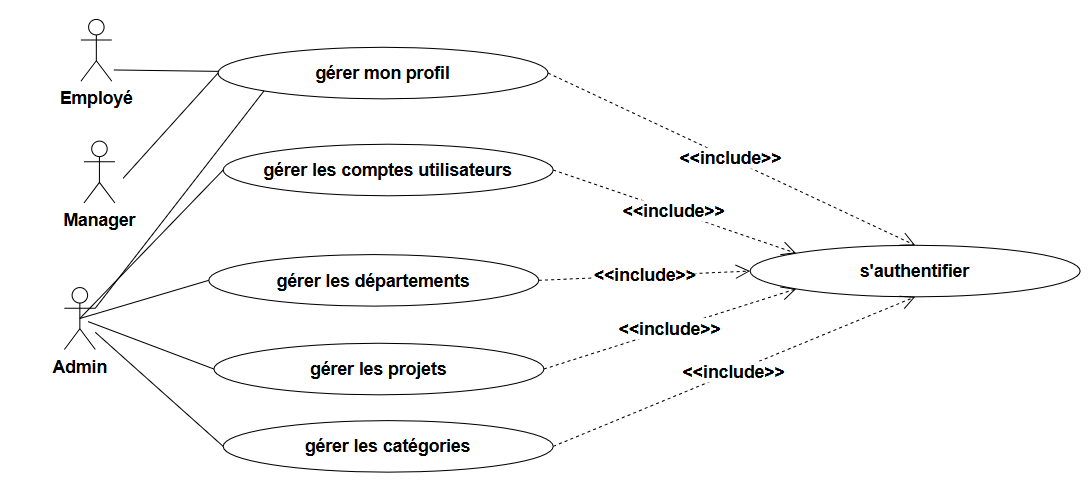
\includegraphics[width=\textwidth]{usecasesp1.png}

 \caption{Diagramme de cas d'utilisation global du sprint 1}

 \label{fig:usecasesp1}

\end{figure}



\subsection{Raffinements des cas d'utilisation}



\subsubsection{Raffinement du cas d'utilisation « Gérer les comptes utilisateurs »}



\begin{figure}[H]

 \centering

 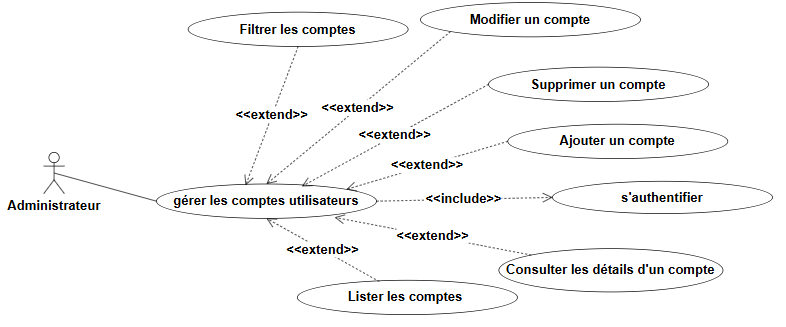
\includegraphics[width=\textwidth]{usecase_raf1.png}

 \caption{Raffinement du cas d'utilisation « Gérer les comptes utilisateurs »}

 \label{fig:gerer_compte}

\end{figure}



\subsubsection{Raffinement du cas d'utilisation « Gérer profil »}



\begin{figure}[H]

 \centering

 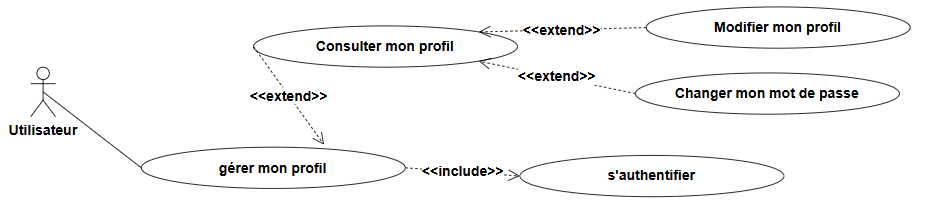
\includegraphics[width=\textwidth]{usecase_raf2.png}

 \caption{Raffinement du cas d'utilisation « Gérer profil »}

 \label{fig:gerer_profil}

\end{figure}



\subsubsection{Raffinement du cas d'utilisation « Gérer les catégories »}



\begin{figure}[H]

 \centering

 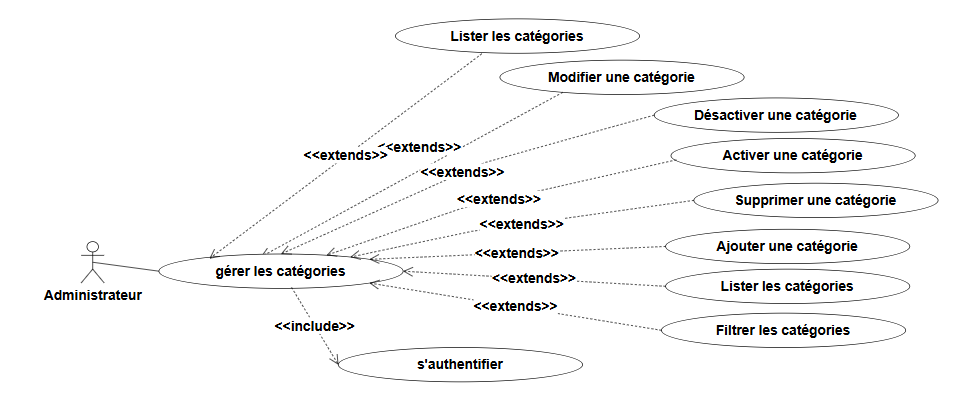
\includegraphics[width=\textwidth]{usecase_raf5.png}

 \caption{Raffinement du cas d'utilisation « Gérer les catégories »}

 \label{fig:gerer_disponibilite}

\end{figure}

\subsubsection{Description textuelle du cas d'utilisation « Créer compte »}



\begin{longtable}{|p{3.5cm}|p{11cm}|}

\caption{Description textuelle « Créer compte »}

\label{tab:create_account_desc}\\

\hline

\textbf{Élément} & \textbf{Description} \\

\hline

\endfirsthead



\hline

\textbf{Élément} & \textbf{Description} \\

\hline

\endhead



\hline

\multicolumn{2}{|c|}{\textit{Suite dans la page suivante}} \\

\hline

\endfoot



\hline

\endlastfoot



Titre & Créer compte utilisateur \\

\hline

Acteur & Administrateur \\

\hline

But & Créer un compte utilisateur et lui envoyer une invitation par email pour qu'il puisse définir son mot de passe \\

\hline

Précondition & L'administrateur est authentifié \\

\hline

\multirow{8}{\linewidth}{Scénario nominal} & 1. L'administrateur accède à la page "Gestion des utilisateurs" \\

& 2. Le système affiche la liste des utilisateurs existants \\

& 3. L'administrateur clique sur "Nouvel utilisateur" \\

& 4. Le système affiche un formulaire de création \\

& 5. L'administrateur saisit : email, prénom, nom, mot de passe, rôle (Employé/Manager/Admin) et département (optionnel) \\

& 6. Il clique sur "Créer" \\

& 7. Le système vérifie que l'email n'est pas déjà utilisé \\

& 8. Le système crée le compte, lui assigne le rôle et envoie un email d'invitation \\

& 9. Un message de succès s'affiche et la liste des utilisateurs est actualisée \\

\hline

\multirow{3}{\linewidth}{Scénario alternatif} & \multicolumn{1}{|p{11cm}|}{6.1 Email déjà existant : le système affiche une erreur "Un utilisateur avec cet email existe déjà" et l'administrateur doit modifier l'email.} \\

& \multicolumn{1}{|p{11cm}|}{8.1 Échec de l'envoi de l'email d'invitation : le compte est tout de même créé, mais l'administrateur est averti et peut renvoyer l'invitation manuellement.} \\

\hline

Post-condition & L'utilisateur est créé dans le système et reçoit un email pour définir son mot de passe \\

\hline

\end{longtable}



\subsubsection{Description textuelle du cas d'utilisation « S'authentifier »}



\begin{longtable}{|p{3.5cm}|p{11cm}|}

\caption{Description textuelle « S'authentifier »}

\label{tab:auth_desc}\\

\hline

\textbf{Élément} & \textbf{Description} \\

\hline

\endfirsthead



\hline

\textbf{Élément} & \textbf{Description} \\

\hline

\endhead



\hline

\multicolumn{2}{|c|}{\textit{Suite dans la page suivante}} \\

\hline

\endfoot



\hline

\endlastfoot



Titre & S'authentifier \\

\hline

Acteur & Utilisateur (Employé, Manager, Administrateur) \\

\hline

But & Accéder à son tableau de bord selon son rôle après identification \\

\hline

Précondition & L'utilisateur possède un compte actif \\

\hline

\multirow{6}{\linewidth}{Scénario nominal} & 1. L'utilisateur accède à la page de connexion \\

& 2. Il saisit son email et son mot de passe \\

& 3. Il clique sur "Se connecter" \\

& 4. Le système vérifie les identifiants \\

& 5. Le système récupère les informations de l'utilisateur (nom, rôle, département) \\

& 6. L'utilisateur est redirigé vers son tableau de bord (Employé / Manager / Admin) \\

\hline

\multirow{3}{\linewidth}{Scénario alternatif} & \multicolumn{1}{|p{11cm}|}{1.1 Première connexion (mot de passe temporaire) : le système redirige automatiquement l'utilisateur vers une page où il doit définir son nouveau mot de passe. Après validation, il est automatiquement connecté.} \\

& \multicolumn{1}{|p{11cm}|}{2.1 Identifiants incorrects : le système affiche un message "Email ou mot de passe invalide" et l'utilisateur reste sur la page de connexion.} \\

& \multicolumn{1}{|p{11cm}|}{3.1 Compte non activé (email non vérifié) : le système affiche un message "Veuillez vérifier votre email pour activer votre compte" et propose de renvoyer l'email d'activation.} \\

\hline

Post-condition & L'utilisateur est connecté et accède à son espace personnel \\

\hline

\end{longtable}



\subsubsection{Description textuelle du cas d'utilisation « Récupérer mot de passe »}



\begin{table}[H]

 \centering

 \caption{Description textuelle « Récupérer mot de passe »}

 \label{tab:forgot_password_desc}

 \begin{tabular}{|p{3.5cm}|p{10.5cm}|}

 \hline

 \textbf{Élément} & \textbf{Description} \\

 \hline

 Titre & Récupérer son mot de passe (Mot de passe oublié) \\

 \hline

 Acteur & Utilisateur \\

 \hline

 But & Réinitialiser son mot de passe en cas d'oubli \\

 \hline

 Précondition & L'utilisateur possède un compte actif avec un email valide \\

 \hline

 \multirow{6}{*} {Scénario nominal} & 1. Sur la page de connexion, l'utilisateur clique sur "Mot de passe oublié ?" \\

 & 2. Il saisit son adresse email \\

 & 3. Le système envoie un email contenant un lien de réinitialisation (valable 24h) \\

 & 4. L'utilisateur clique sur le lien reçu \\

 & 5. Il saisit et confirme son nouveau mot de passe \\

 & 6. Le système met à jour le mot de passe et redirige l'utilisateur vers la page de connexion \\

 \hline

 \multirow{3}{*} {Scénario alternatif} & 2.1. Email non trouvé : le système affiche un message générique "Si un compte existe avec cet email, vous recevrez un lien de réinitialisation" (mesure de sécurité). \\

 & 5.1 Mots de passe non concordants : le système affiche une erreur et demande à l'utilisateur de ressaisir son nouveau mot de passe. \\

 & 4.1 Lien expiré (plus de 24h) : le système affiche un message d'erreur et propose à l'utilisateur de refaire une demande de réinitialisation. \\

 \hline

 Post-condition & Le mot de passe de l'utilisateur est modifié avec succès \\

 \hline

 \end{tabular}

\end{table}



\subsubsection{Description textuelle du cas d'utilisation « Modifier son profil »}



\begin{table}[H]

 \centering

 \caption{Description textuelle « Modifier son profil »}

 \label{tab:profile_desc}

 \begin{tabular}{|p{3.5cm}|p{11cm}|}

 \hline

 \textbf{Élément} & \textbf{Description} \\

 \hline

 Titre & Modifier son profil \\

 \hline

 Acteur & Utilisateur \\

 \hline

 But & Consulter et modifier ses informations personnelles (prénom, nom) \\

 \hline

 Précondition & L'utilisateur est authentifié \\

 \hline

 \multirow{6}{*} {Scénario nominal} & 1. L'utilisateur clique sur son nom/avatar dans la barre de navigation \\

 & 2. Il sélectionne "Mon profil" dans le menu déroulant \\

 & 3. Le système affiche la page de profil avec les informations actuelles \\

 & 4. L'utilisateur clique sur "Modifier" \\

 & 5. Il modifie son prénom et/ou son nom \\

 & 6. Il clique sur "Enregistrer" \\

 & 7. Le système valide les données et met à jour le profil \\

 & 8. Un message de succès s'affiche et la page se recharge avec les nouvelles informations \\

 \hline

 \multirow{3}{*} {Scénario alternatif} 

 & 6.1 Données invalides (caractères spéciaux non autorisés) : le système affiche un message d'erreur détaillé. \\

 & 5.1 Tentative de modification de l'email : le champ email est désactivé (lecture seule) avec le message "L'email ne peut être modifié que par l'administrateur". \\

 \hline

 Post-condition & Les informations du profil sont mises à jour dans le système \\

 \hline

 \end{tabular}

\end{table}



\subsubsection{Description textuelle du cas d'utilisation « Ajouter une catégorie »}



\begin{longtable}{|p{3.5cm}|p{11cm}|}

\caption{Description textuelle « Ajouter une catégorie »}

\label{tab:category_desc}\\

\hline

\textbf{Élément} & \textbf{Description} \\

\hline

\endfirsthead



\hline

\textbf{Élément} & \textbf{Description} \\

\hline

\endhead



\hline

\multicolumn{2}{|c|}{\textit{Suite dans la page suivante}} \\

\hline

\endfoot



\hline

\endlastfoot



Titre & Ajouter une catégorie \\

\hline

Acteur & Administrateur \\

\hline

But & Créer une catégorie de dépenses avec des champs personnalisés \\

\hline

Précondition & L'administrateur est authentifié \\

\hline

\multirow{8}{\linewidth}{Scénario nominal} & 1. L'administrateur accède à la page "Gestion des catégories" \\

& 2. Le système affiche la liste des catégories existantes \\

& 3. L'administrateur clique sur "Ajouter une catégorie" \\

& 4. Il saisit le nom de la catégorie (ex: Transport, Hébergement) et le plafond de remboursement \\

& 5. Il ajoute des champs personnalisés (nom, type: texte/nombre/date/choix, requis ou non) \\

& 6. L'administrateur clique sur "Créer" \\

& 7. Le système vérifie que le nom de la catégorie est unique \\

& 8. Le système enregistre la catégorie et ses champs \\

& 9. Un message de succès s'affiche et la liste des catégories est actualisée \\

\hline

\multirow{3}{\linewidth}{Scénario alternatif} & \multicolumn{1}{|p{11cm}|}{7.1 Nom de catégorie déjà existant : le système affiche une erreur "Une catégorie avec ce nom existe déjà" et l'administrateur doit choisir un autre nom.} \\

& \multicolumn{1}{|p{11cm}|}{6.1 Champ SELECT créé sans options : le système affiche une erreur "Les options sont requises pour un champ de type liste déroulante" et bloque la création.} \\

& \multicolumn{1}{|p{11cm}|}{5.1 Nom de champ personnalisé déjà utilisé dans une autre catégorie : le système propose de réutiliser le champ existant (avec le même type) plutôt que d'en créer un nouveau.} \\

\hline

Post-condition & La catégorie est créée et ses champs sont disponibles dans les formulaires de notes de frais \\

\hline

\end{longtable}





\section{Conception}

\subsection{Diagramme de séquence}



\subsubsection{Diagramme de séquence - S'authentifier}



\begin{figure}[H]

\centering

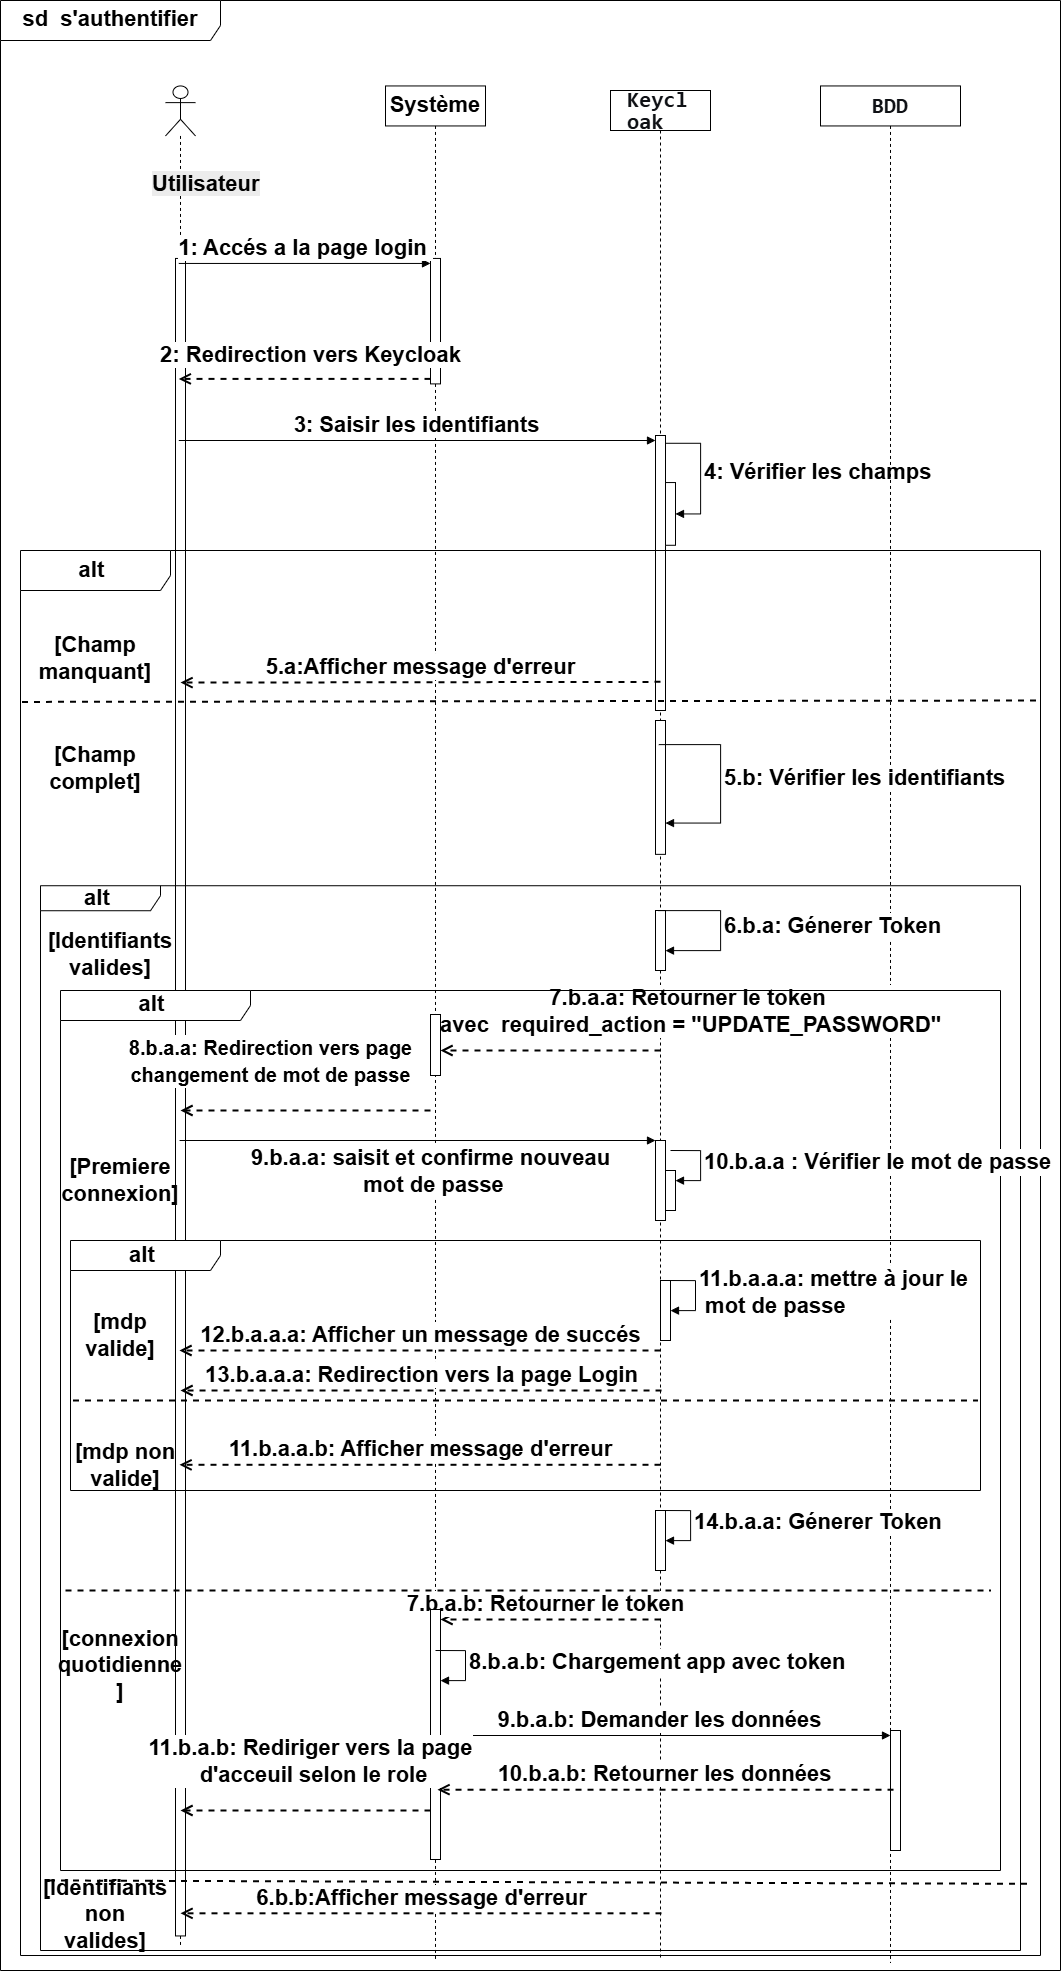
\includegraphics[

 width=\textwidth,

 keepaspectratio,

 height=0.80\textheight % Réduit à 45% de la page

]{authentification.png}

 \caption{Diagramme de séquence - S'authentifier}

 \label{fig:seq_auth}

\end{figure}



\subsubsection{Diagramme de séquence - Ajouter un projet}



\begin{figure}[H]

 \centering

 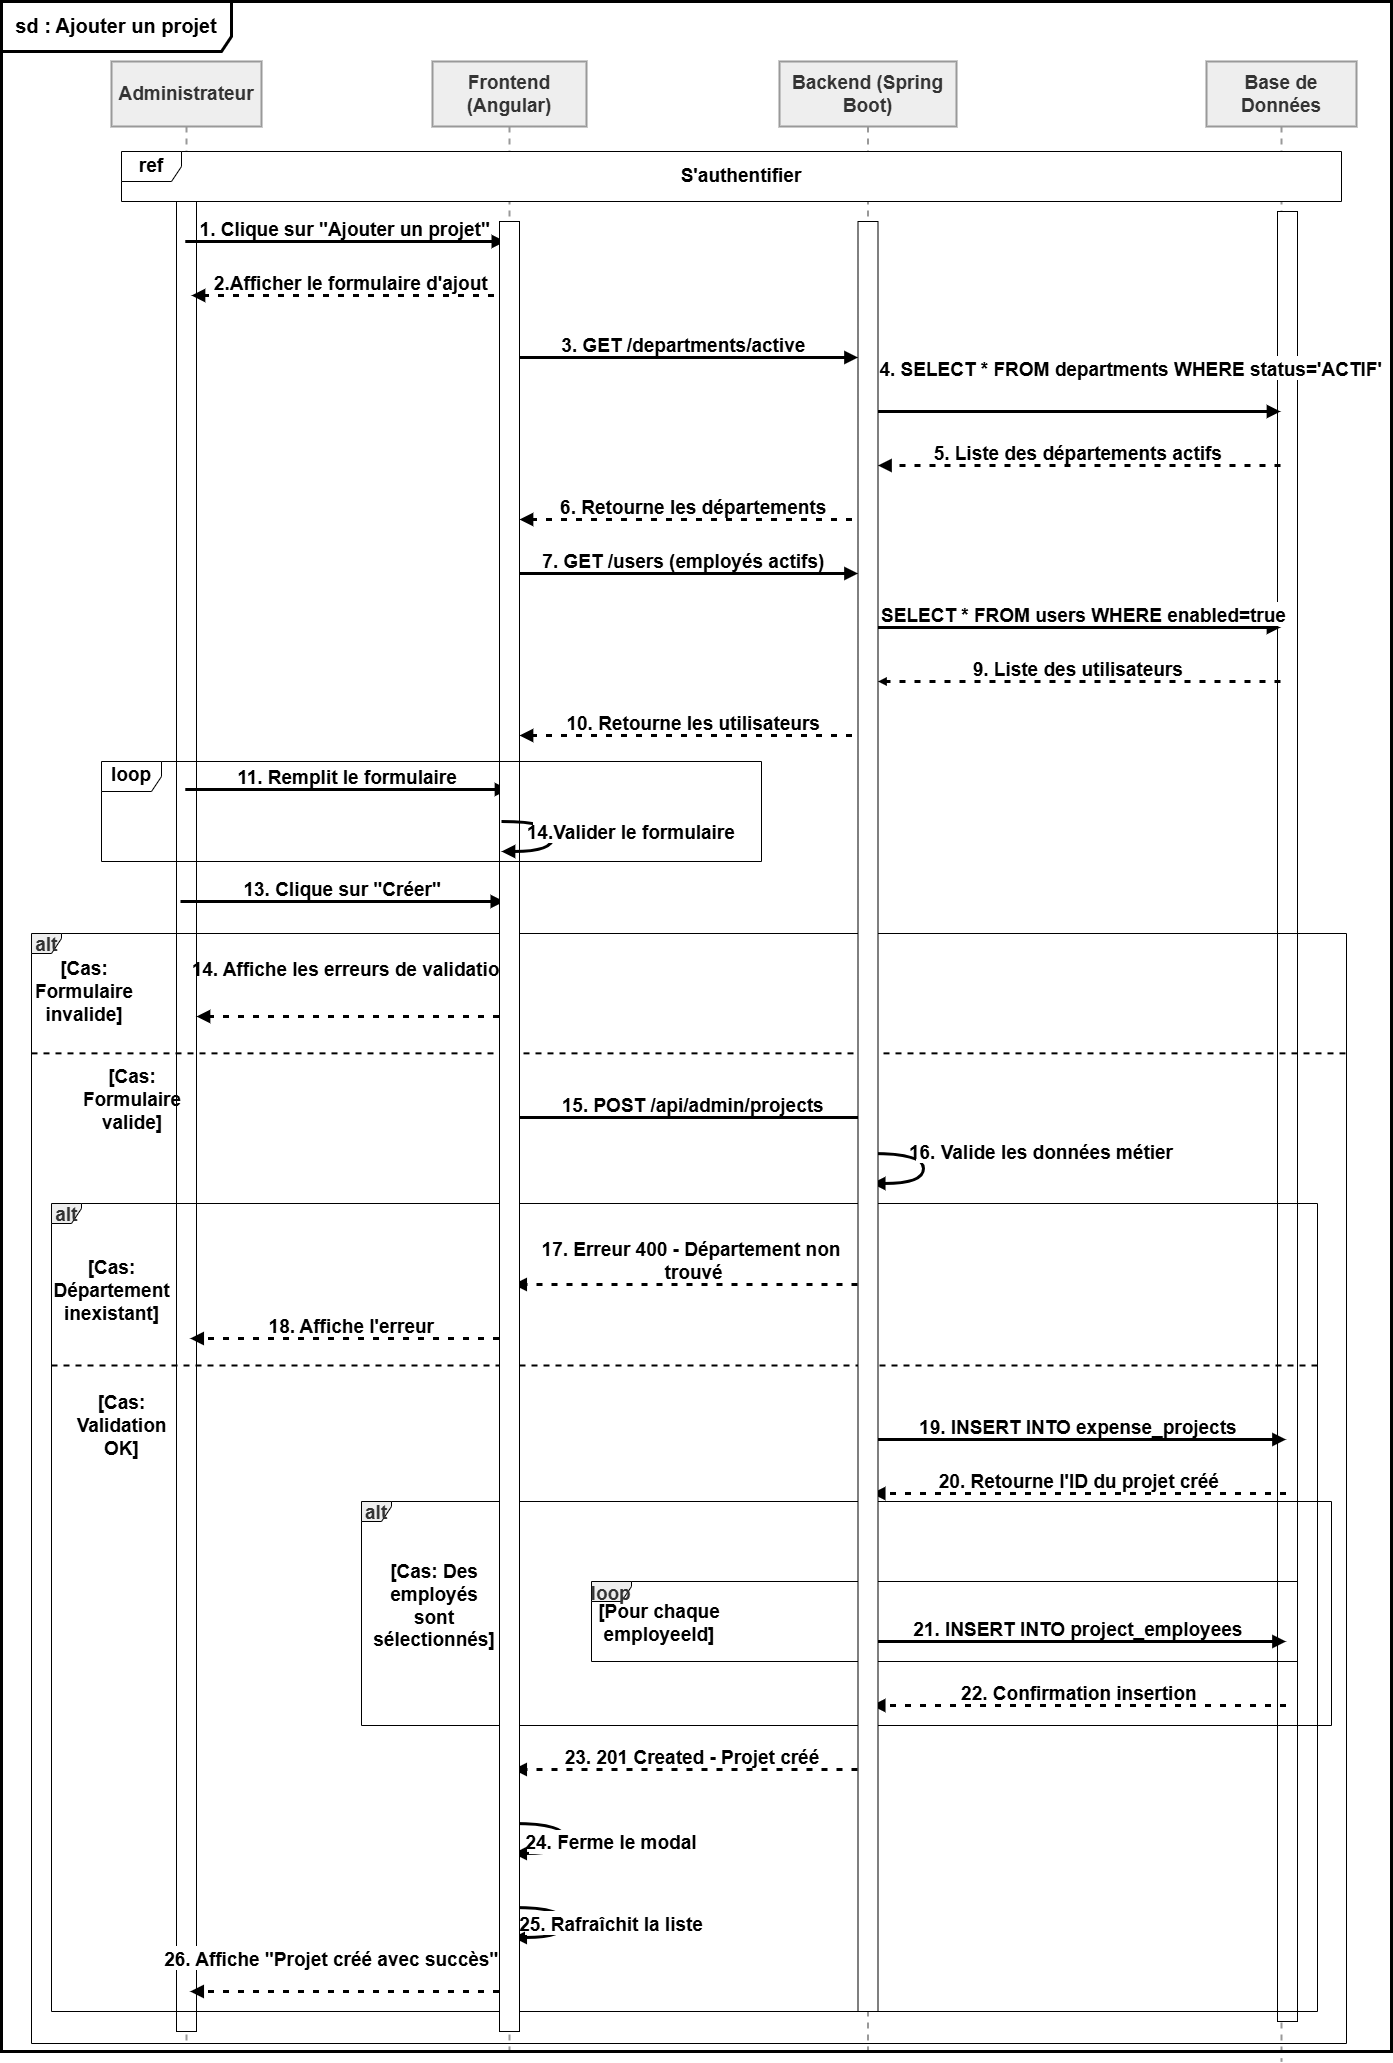
\includegraphics[width=1\textwidth,height=0.85\textheight]{seq_project2.png}

 \caption{Diagramme de séquence - Ajouter un projet}

 \label{fig:seq_project}

\end{figure}

\subsubsection{Diagramme de séquence - Ajouter une catégorie}



\begin{figure}[H]

 \centering

 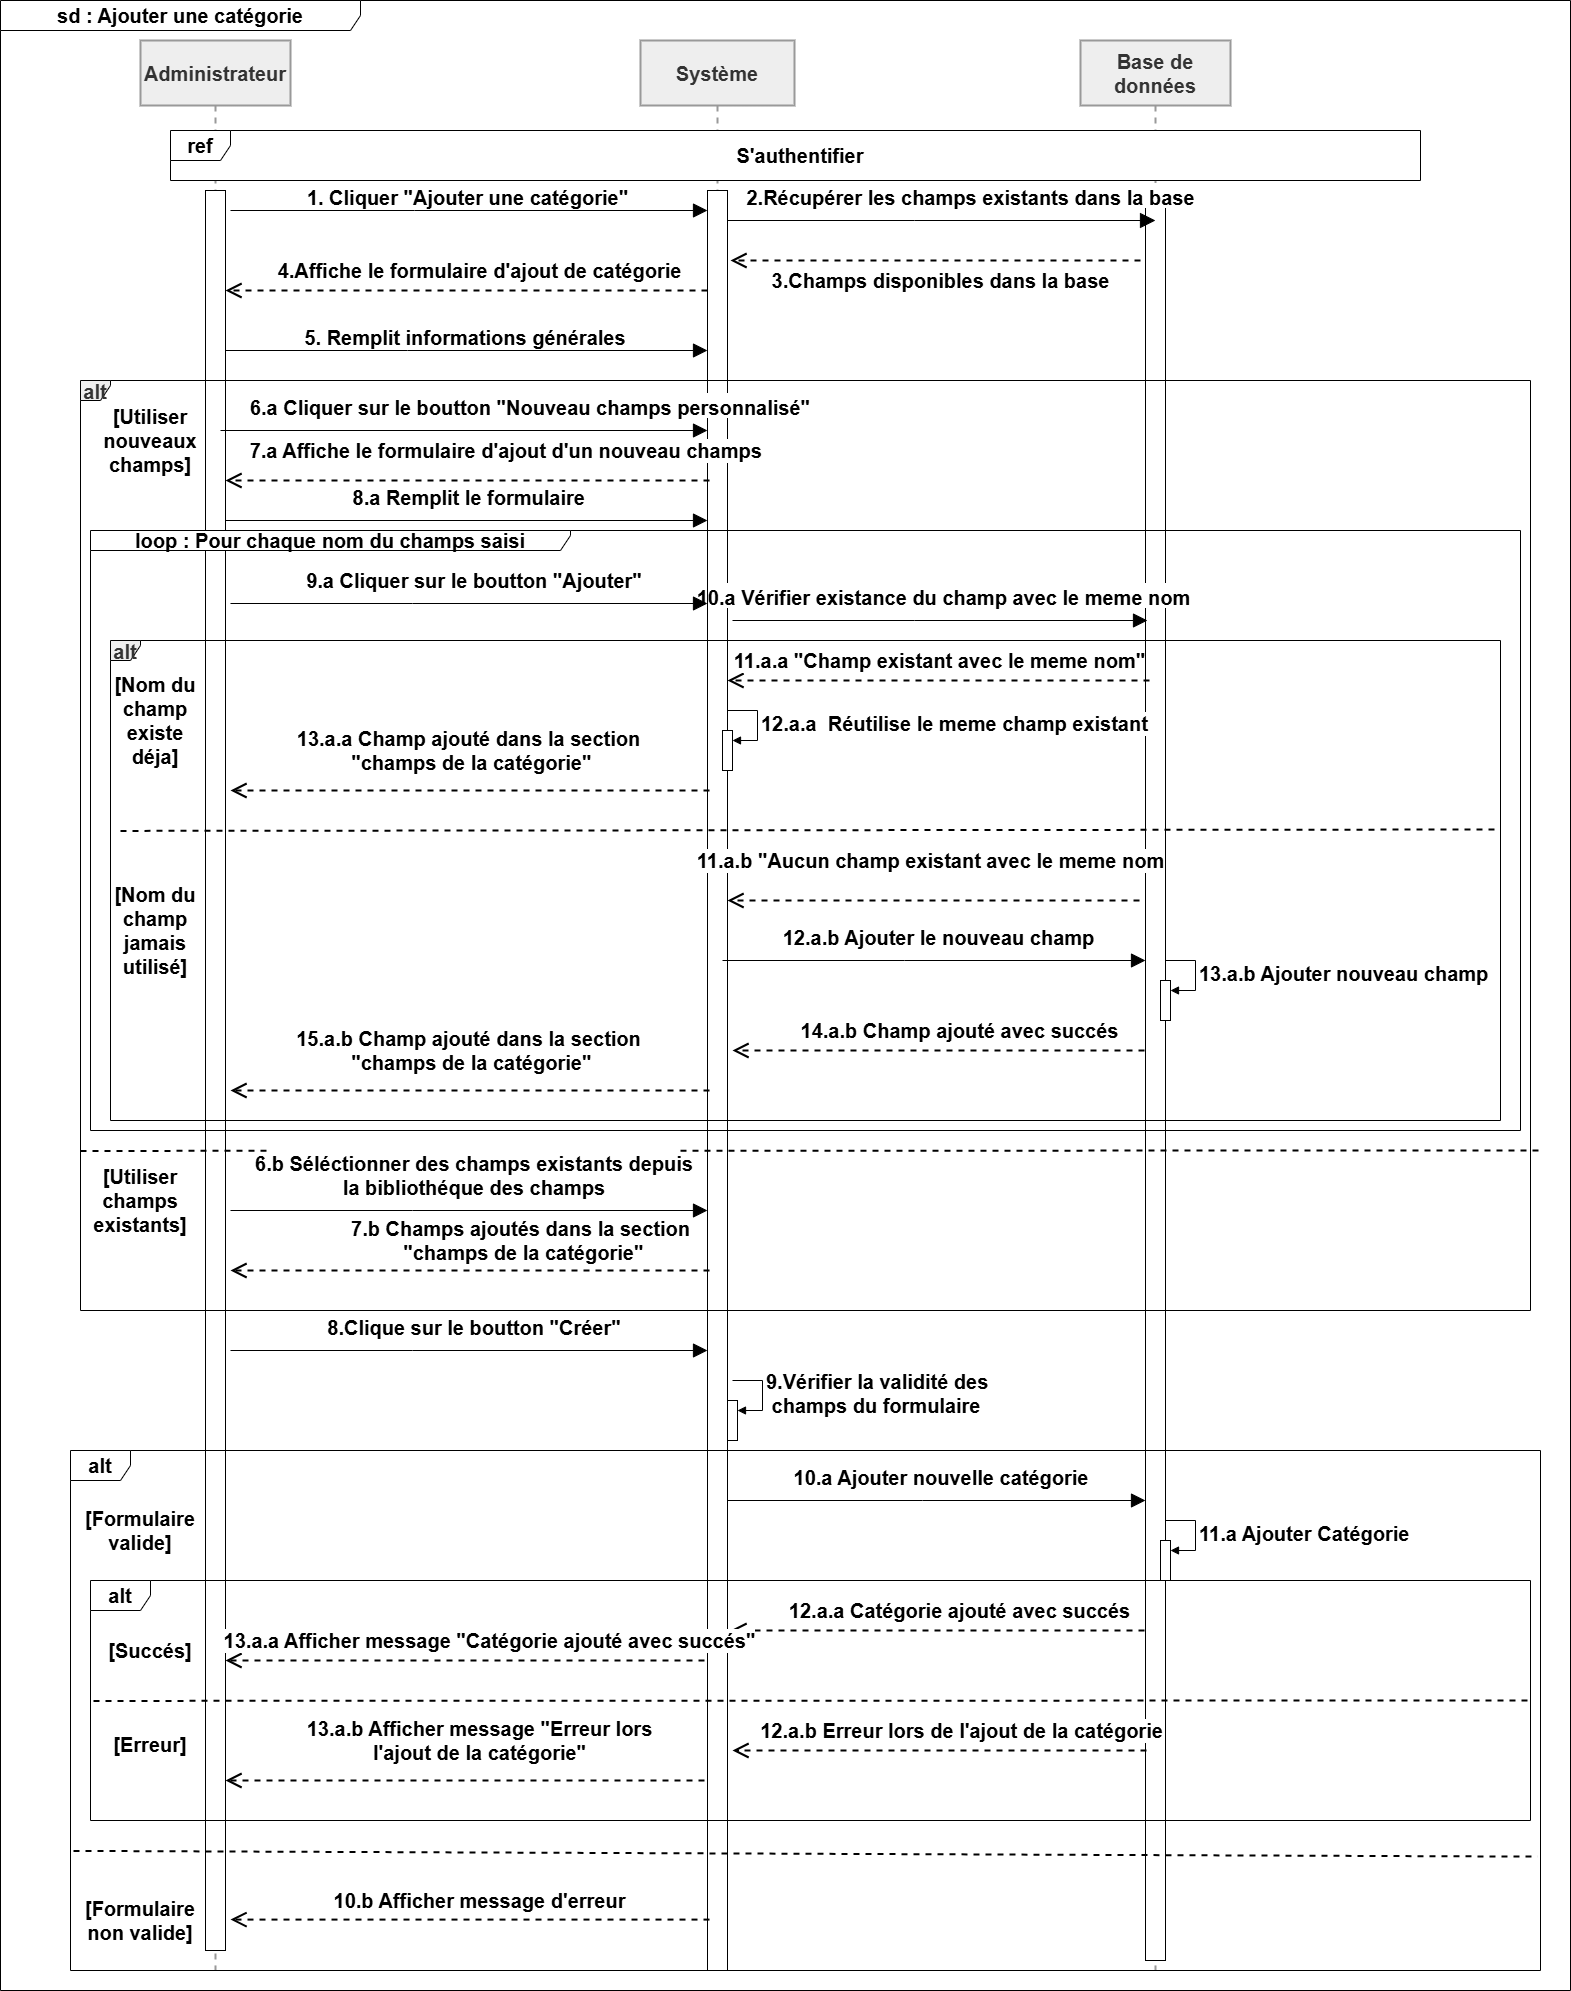
\includegraphics[width=1\textwidth,height=0.92\textheight]{seq_category.png}

 \caption{Diagramme de séquence - Ajouter une catégorie}

 \label{fig:seq_category}

\end{figure}

\subsection{Diagramme de classe du sprint 1}

Ce diagramme présente les entités principales du sprint 1 et leurs relations.

\begin{figure}[H]

 \centering

 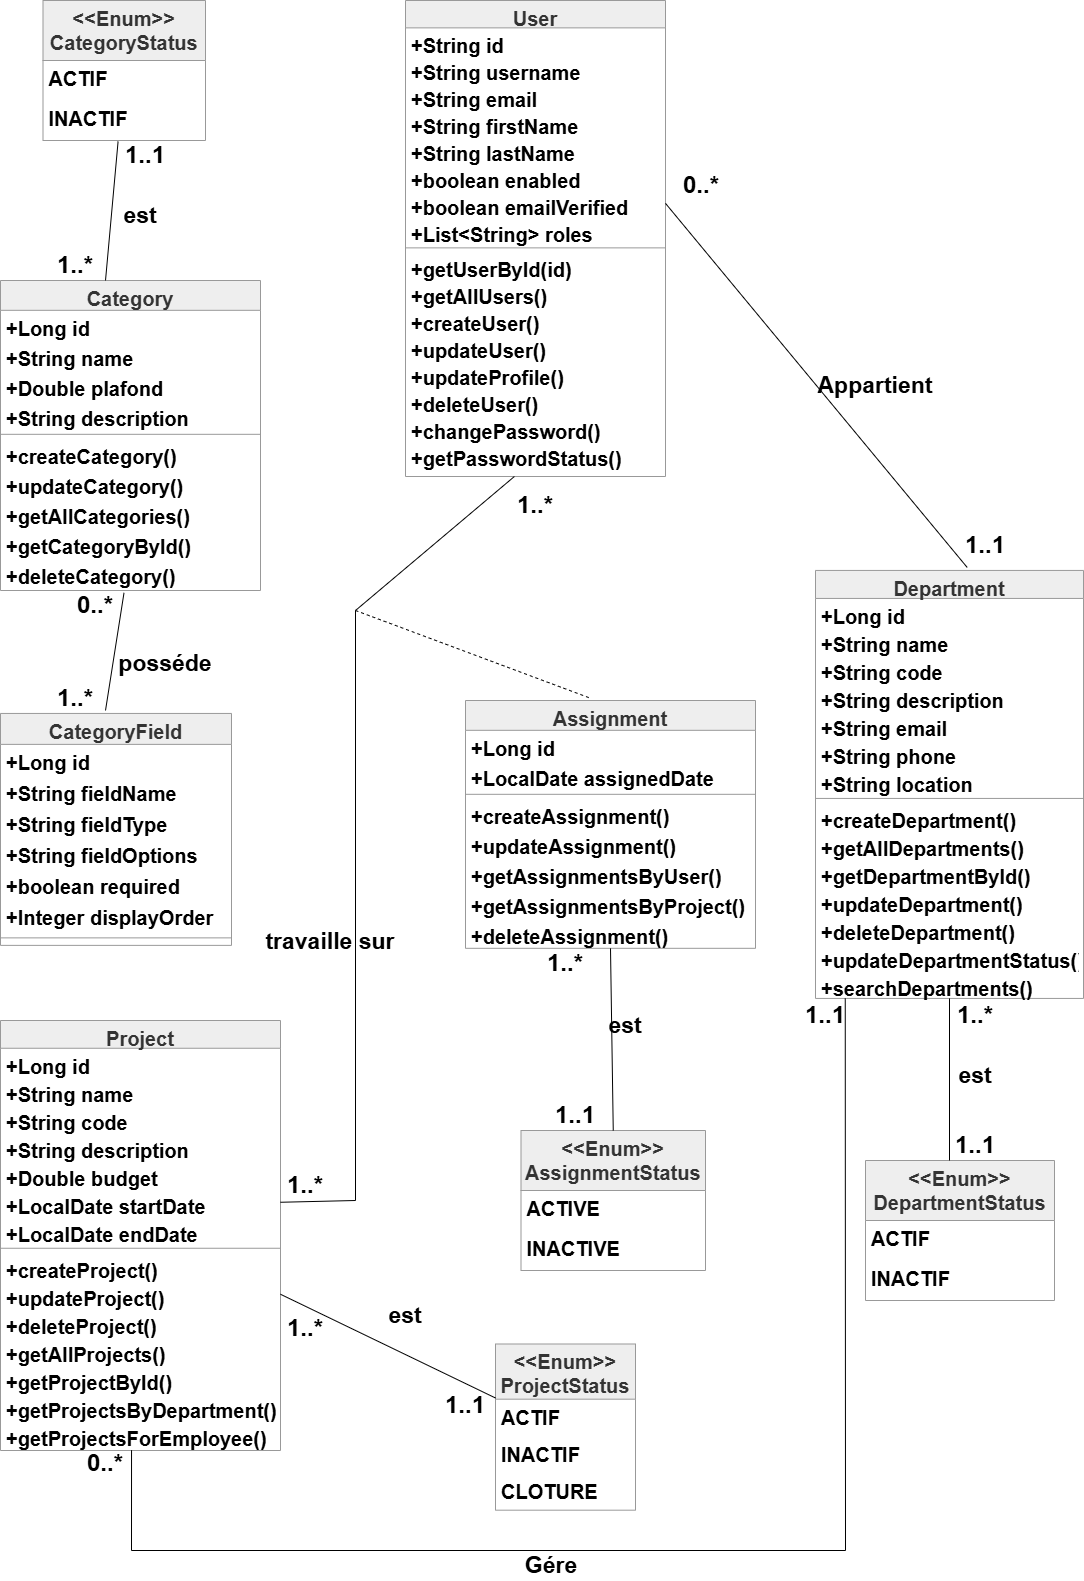
\includegraphics[width=0.85\textwidth,height=0.86\textheight]{diagclassesprint1.png}

 \caption{Diagramme de classes du sprint 1}

 \label{fig:class_sprint1}

\end{figure}







\section{Interfaces développées}



\subsection{Page d'accueil}

La page d'accueil de Coral-io est une landing page professionnelle qui présente l'entreprise et ses services aux visiteurs. Elle permet aux utilisateurs non authentifiés de découvrir l'application avant de se connecter.



Depuis cette interface, le visiteur peut :

\begin{itemize}

 \item Naviguer entre les différentes sections : Acceuil, A propos, Caractéristiques, Services, Contact

 \item Consulter la présentation de l'entreprise Coral-io et ses valeurs

 \item Découvrir les services proposés (DevOps, APM, Intégration des solutions tiers, Finance et Assurance)

 \item Visualiser les témoignages clients et les statistiques de l'entreprise

 \item Accéder à la section FAQ pour trouver des réponses aux questions fréquentes

 \item Contacter l'entreprise via le formulaire de contact

 \item Cliquer sur le bouton "Connexion" pour accéder à la page d'authentification

\end{itemize}



La page intègre une navigation responsive, des animations au défilement, et un design moderne avec des illustrations et des icônes.



\begin{figure}[H]

 \centering

 
\includegraphics[width=\textwidth]{home-hero.png}

 \caption{Page d'accueil}

 \label{fig:interface_home_hero}

\end{figure}



\begin{figure}[H]

 \centering

 
\includegraphics[width=\textwidth]{home-about.png}

 \caption{Page d'accueil - Section A propos}

 \label{fig:interface_home_about}

\end{figure}

\begin{figure}[H]

 \centering

 
\includegraphics[width=\textwidth]{home-expertise.png}

 \caption{Page d'accueil - Section Expertises}

 \label{fig:interface_home_expertise}

\end{figure}

\begin{figure}[H]

 \centering

 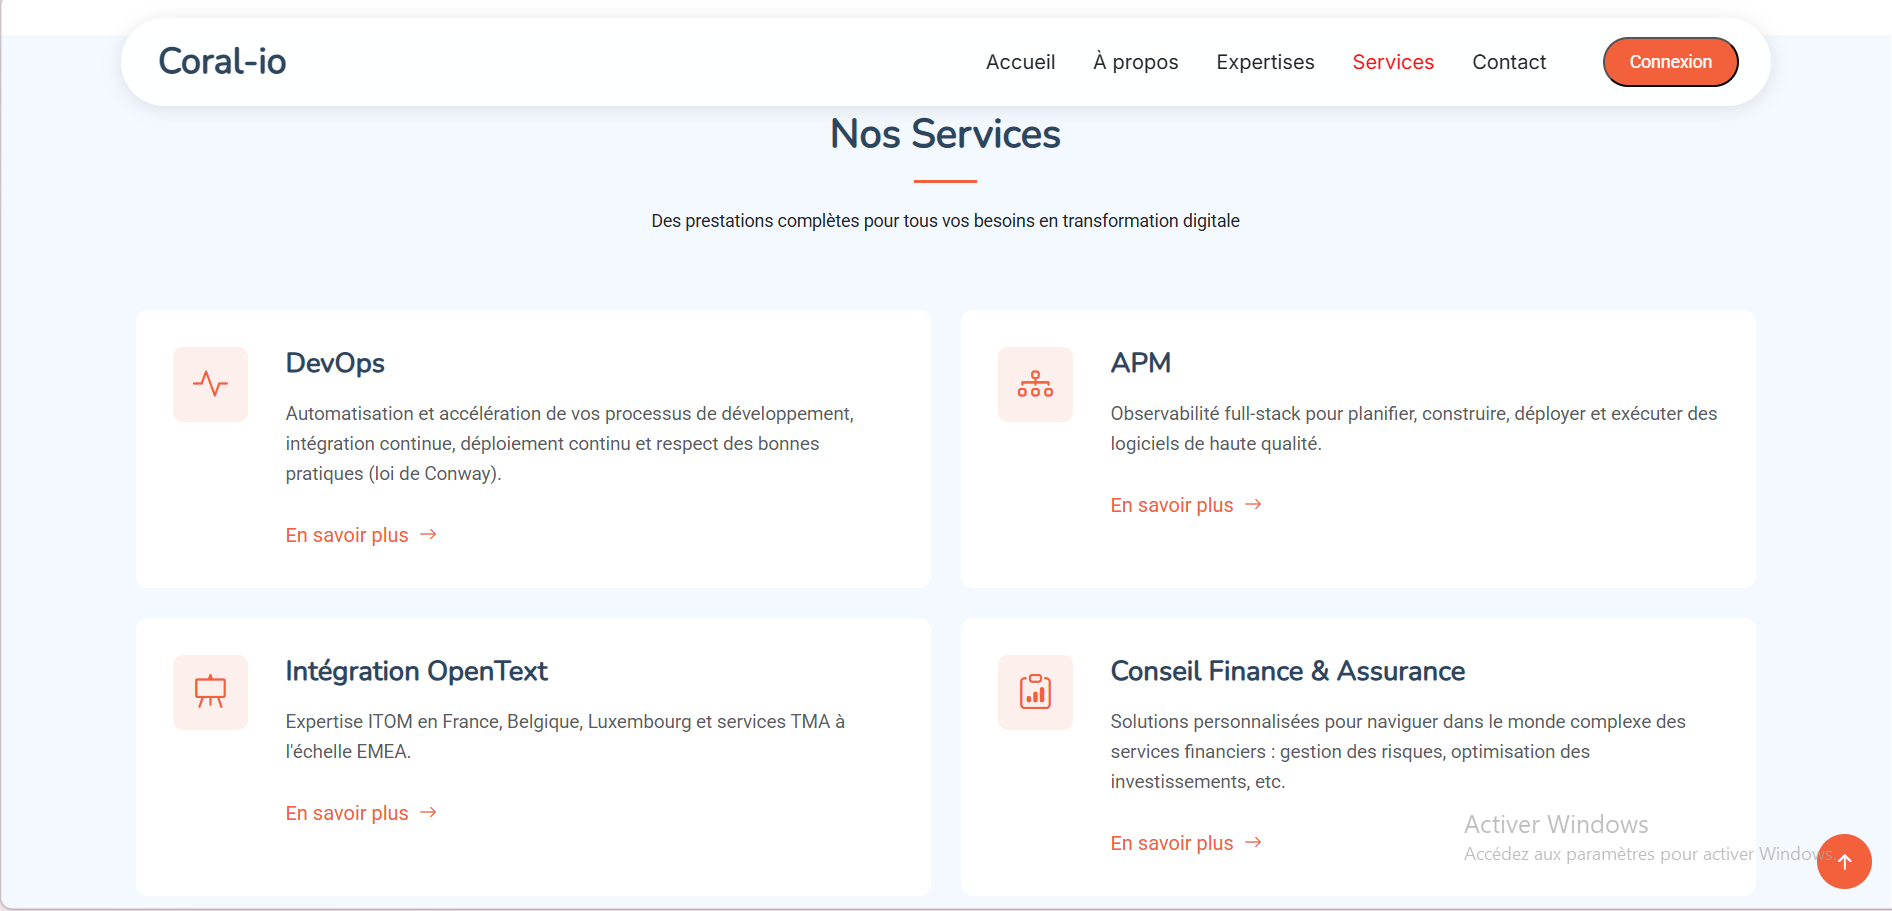
\includegraphics[width=\textwidth]{home-services.png}

 \caption{Page d'accueil - Section Services}

 \label{fig:interface_home_services}

\end{figure}



\begin{figure}[H]

 \centering

 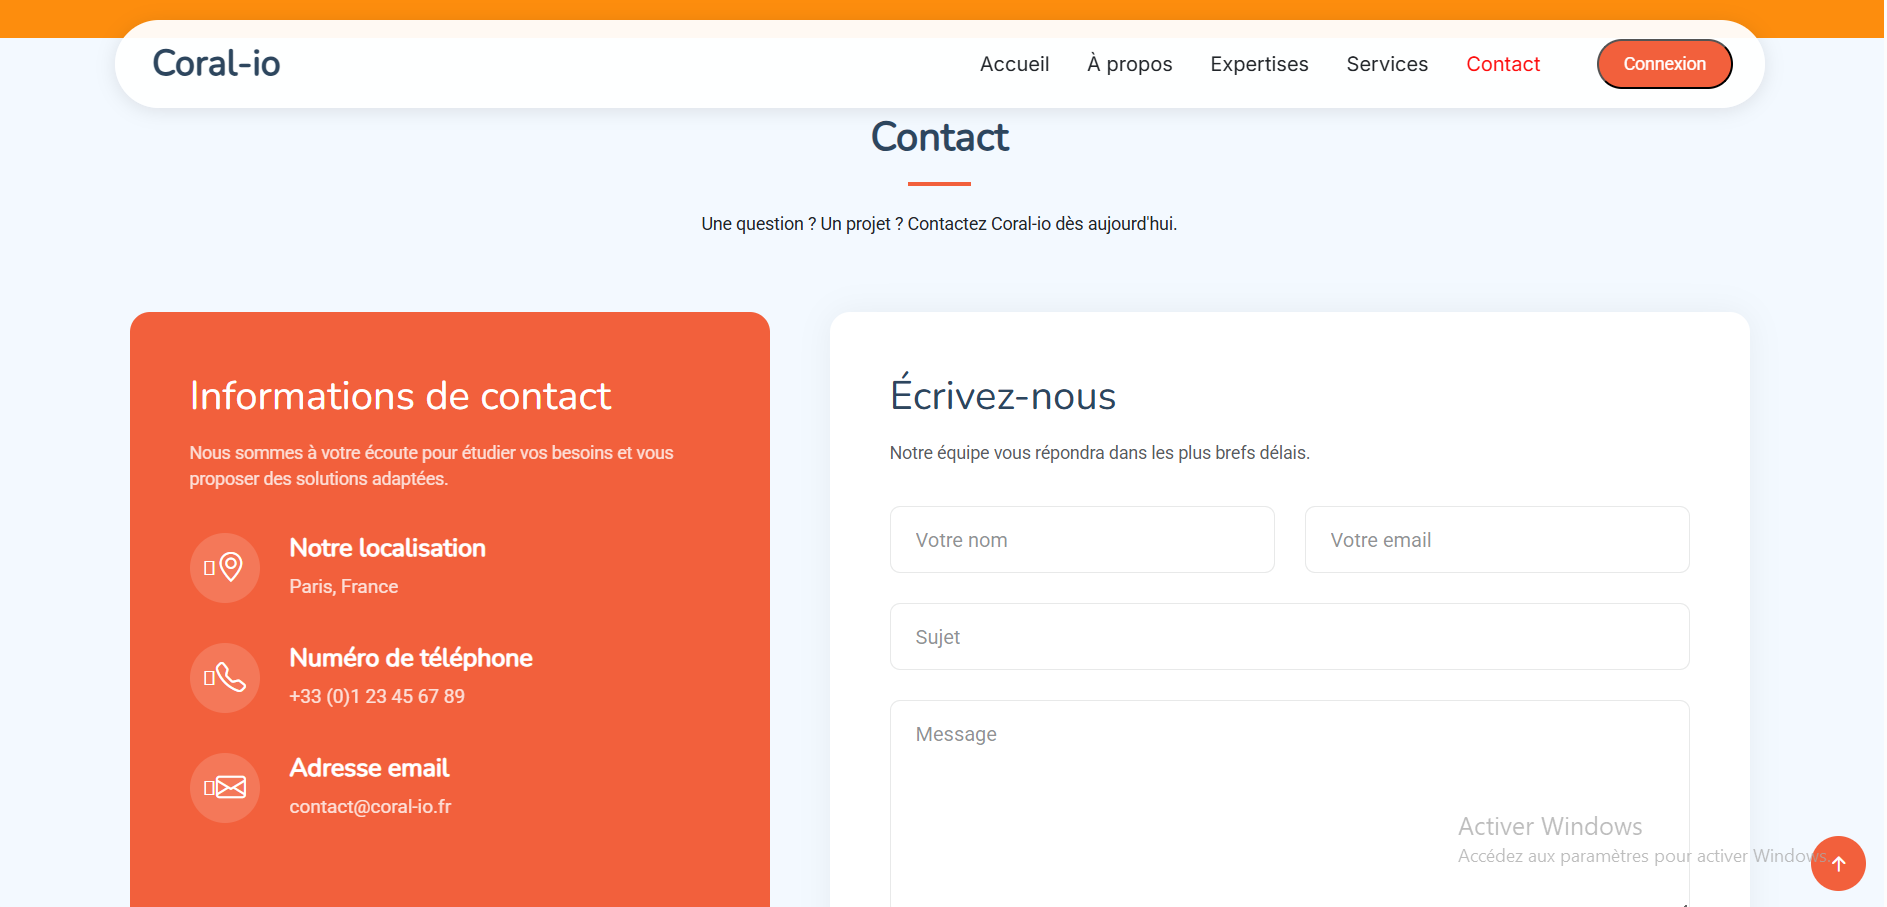
\includegraphics[width=\textwidth]{home-contact.png}

 \caption{Page d'accueil - Section Contact}

 \label{fig:interface_home_contact}

\end{figure}



\subsection{Interface d'authentification}

Si l'utilisateur n'est pas authentifié, c'est l'interface d'authentification qui s'affiche en premier. L'utilisateur saisit son email (ou nom d'utilisateur) et son mot de passe, puis clique sur le bouton "Se connecter". Le système vérifie la validité des informations saisies via Keycloak et affiche un message d'erreur si elles sont incorrectes. En cas de succès, l'utilisateur est redirigé vers son tableau de bord selon son rôle (Employé, Manager ou Administrateur). Si l'utilisateur a oublié son mot de passe, il peut cliquer sur le lien "Réinitialiser le mot de passe" pour accéder à la page de récupération. Une option "Se souvenir de moi" permet de rester connecté sur le navigateur.



\begin{figure}[H]

 \centering

 
\includegraphics[width=\textwidth]{interface_login.png}

 \caption{Interface d'authentification}

 \label{fig:interface_login}

\end{figure}



\subsection{Interface de récupération de mot de passe}

Cette interface permet à l'utilisateur de demander la réinitialisation de son mot de passe en cas d'oubli. L'utilisateur saisit son nom d'utilisateur ou son email, puis clique sur le bouton "Envoyer". Le système vérifie l'existence du compte et envoie un email contenant un lien de réinitialisation temporaire (valable 24h). Un message de succès s'affiche pour confirmer l'envoi, ou un message d'erreur si l'email n'existe pas. Un lien "Retour à la connexion" permet de revenir à la page d'authentification.



\begin{figure}[H]

 \centering

 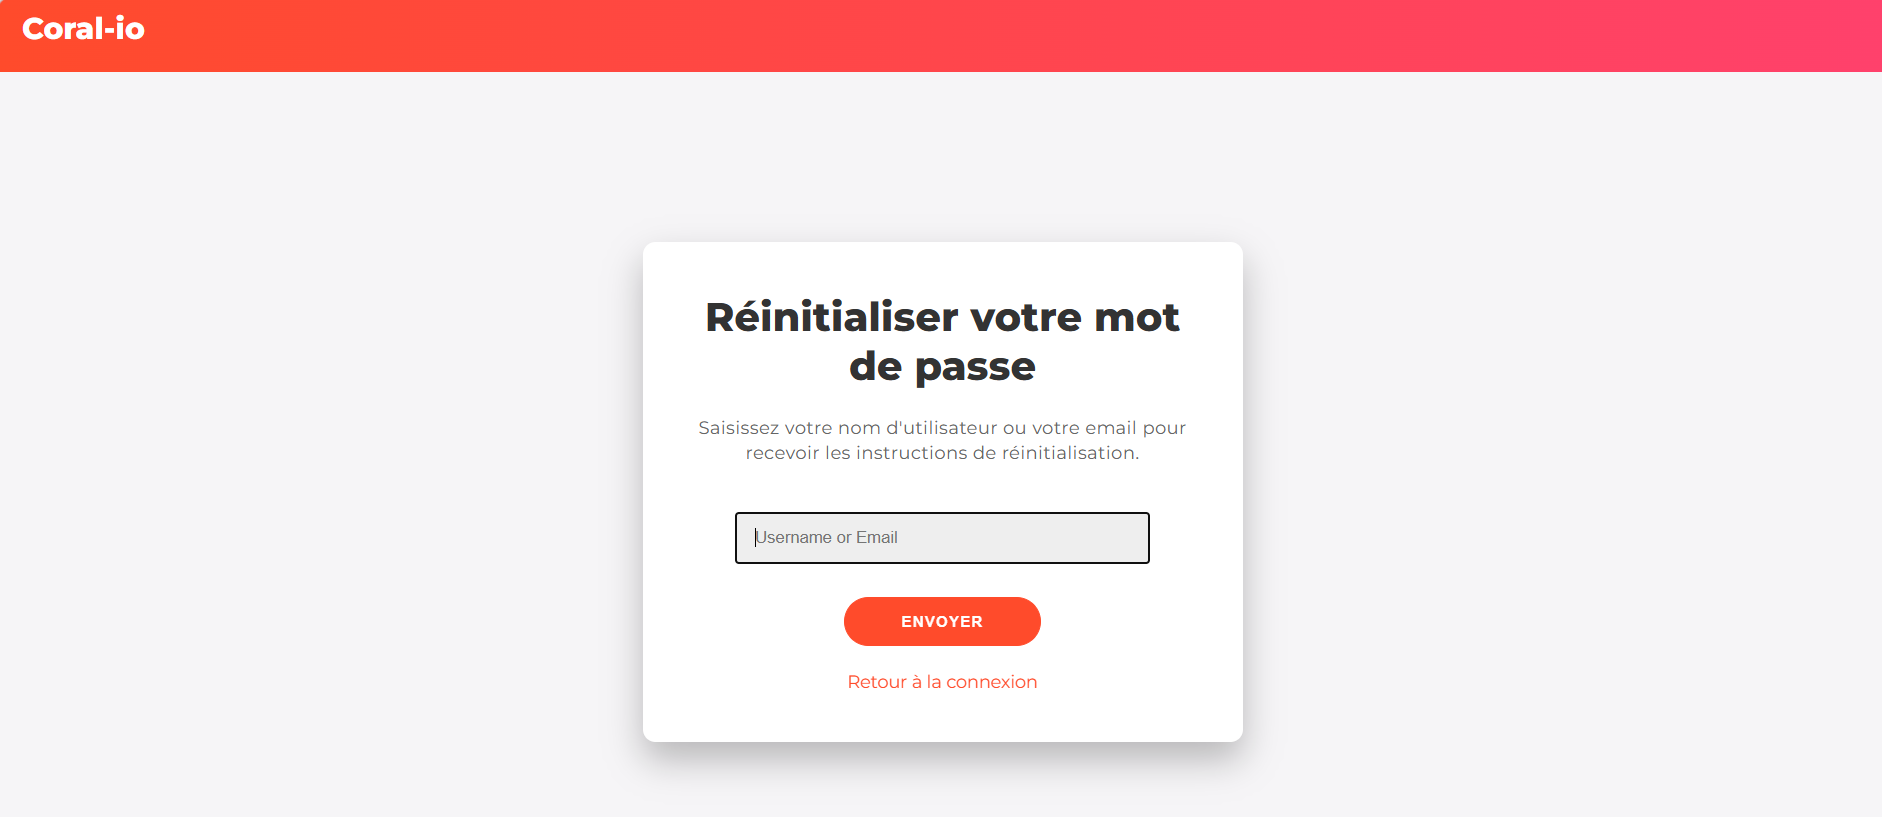
\includegraphics[width=\textwidth]{interface_reset_password.png}

 \caption{Interface de récupération de mot de passe}

 \label{fig:interface_reset_password}

\end{figure}



\subsection{Interface de création/mise à jour du mot de passe}

Cette interface unifiée s'affiche dans deux cas : après avoir cliqué sur le lien de réinitialisation reçu par email, ou lors de la première connexion d'un compte créé par l'administrateur. L'utilisateur saisit son nouveau mot de passe, le confirme, puis clique sur "Mettre à jour". Le système valide la correspondance des mots de passe et le respect des règles de sécurité (minimum 6 caractères). En cas d'erreur, un message rouge s'affiche. Après validation, l'utilisateur est automatiquement authentifié et redirigé vers son tableau de bord.



\begin{figure}[H]

 \centering

 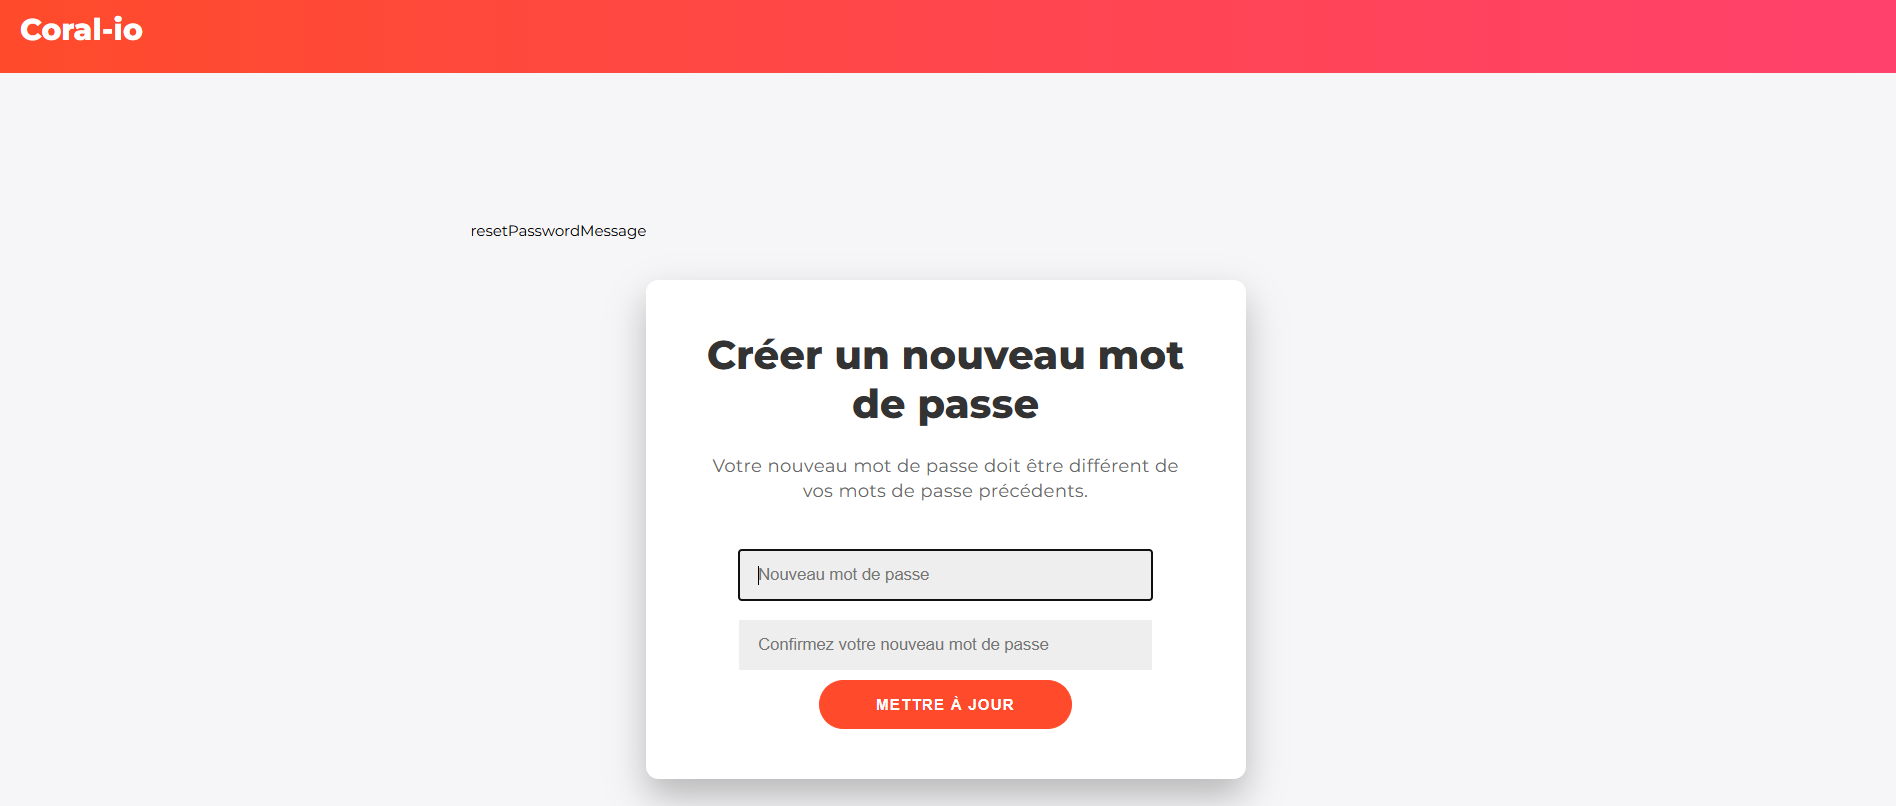
\includegraphics[width=\textwidth]{interface_update_password.png}

 \caption{Interface de création/mise à jour du mot de passe}

 \label{fig:interface_update_password}

\end{figure}

\subsection{Interface de mise à jour du profil utilisateur}

Cette interface s’affiche lorsque l’utilisateur se connecte pour la première fois et que l’administrateur n’a pas renseigné ses informations personnelles (nom, prénom) lors de la création de son compte. Elle permet à l’utilisateur de compléter son profil avant d’accéder à la plateforme. L’utilisateur saisit ses informations, puis clique sur le bouton « update ». Le système valide que tous les champs obligatoires sont remplis. En cas d’erreur, un message s’affiche. Après validation, les données sont enregistrées et l’utilisateur est redirigé vers son tableau de bord.



\begin{figure}[H]

 \centering

 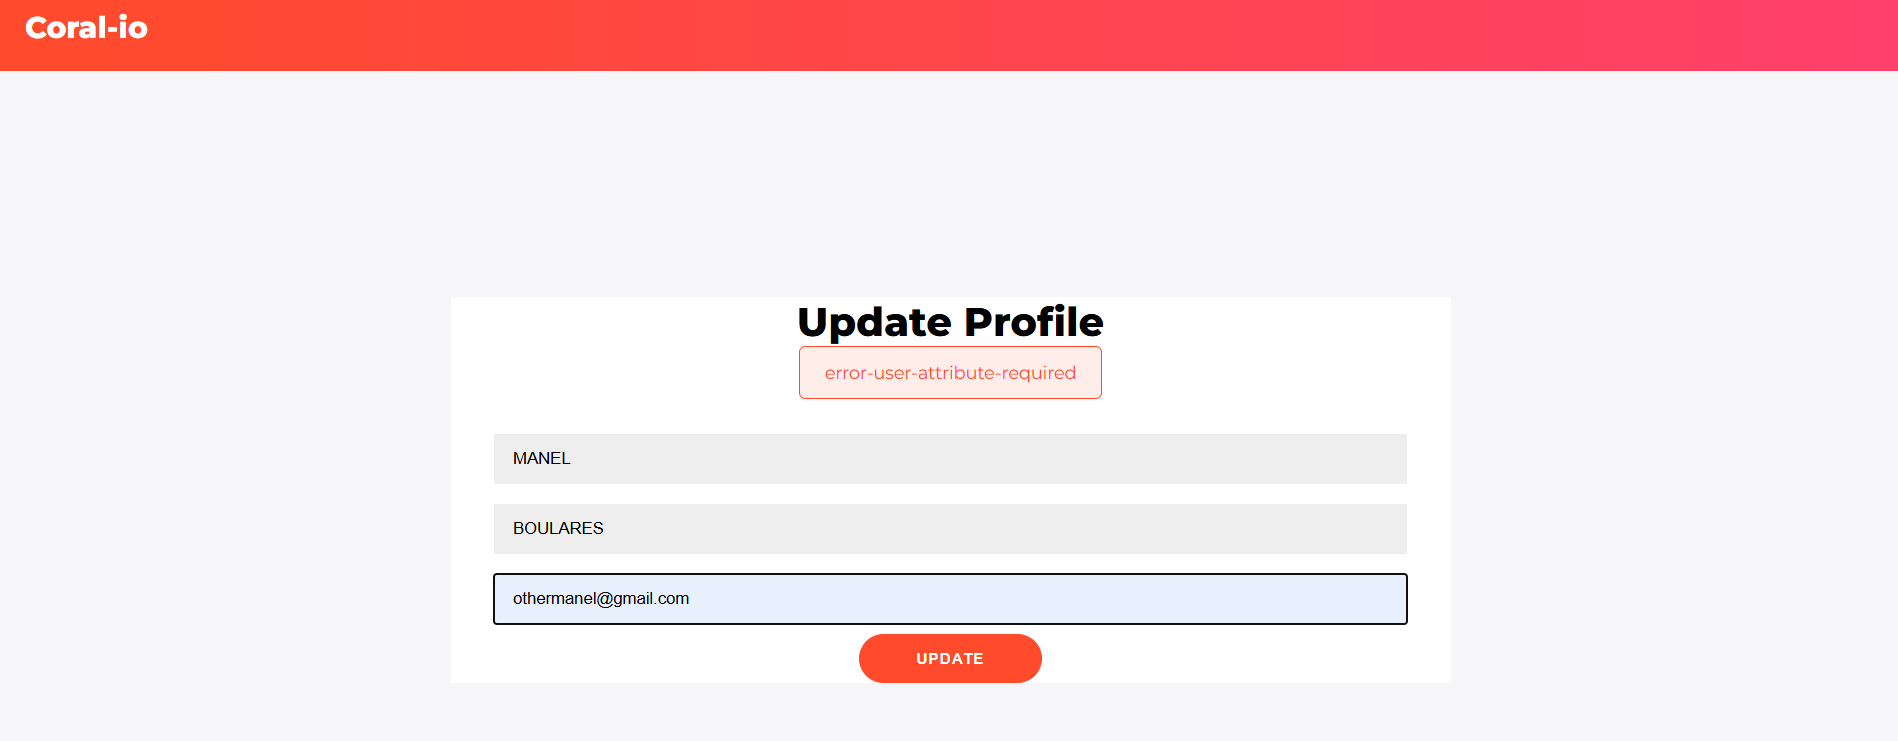
\includegraphics[width=\textwidth]{interface_update_profile.png}

 \caption{Interface de mise à jour du profil utilisateur}

 \label{fig:interface_update_profile}

\end{figure}



\subsection{Modal de confirmation de déconnexion}

Ce modal s’affiche lorsque l’utilisateur clique sur le bouton de déconnexion, afin d’éviter toute déconnexion accidentelle. Une fenêtre de dialogue apparaît avec le message « Voulez-vous vraiment vous déconnecter ? » accompagné de deux boutons : « Annuler » (ferme le modal sans déconnecter) et « Oui » (déconnecte l’utilisateur et le redirige vers la page d’authentification). Ce mécanisme améliore la sécurité et l’expérience utilisateur en prévenant les actions involontaires.



\begin{figure}[H]

 \centering

 
\includegraphics[width=\textwidth]{modal_logout.png}

 \caption{Modal de confirmation de déconnexion}

 \label{fig:modal_logout}

\end{figure}

\subsection{Gestion des utilisateurs par l'administrateur}



\subsubsection{Interface de liste des utilisateurs}

En tant qu'administrateur, il a la possibilité de visualiser tous les utilisateurs de l'application via une liste paginée avec des statistiques (total, actifs, inactifs, départements). Il peut filtrer les utilisateurs par rôle (Manager/Employé), par département et par statut (actif/inactif), rechercher un utilisateur par nom, email ou nom d'utilisateur, voir ses détails, modifier ses informations, le supprimer après confirmation ou exporter la liste. Un bouton « Nouvel utilisateur » permet d'accéder au formulaire de création.



\begin{figure}[H]

 \centering

 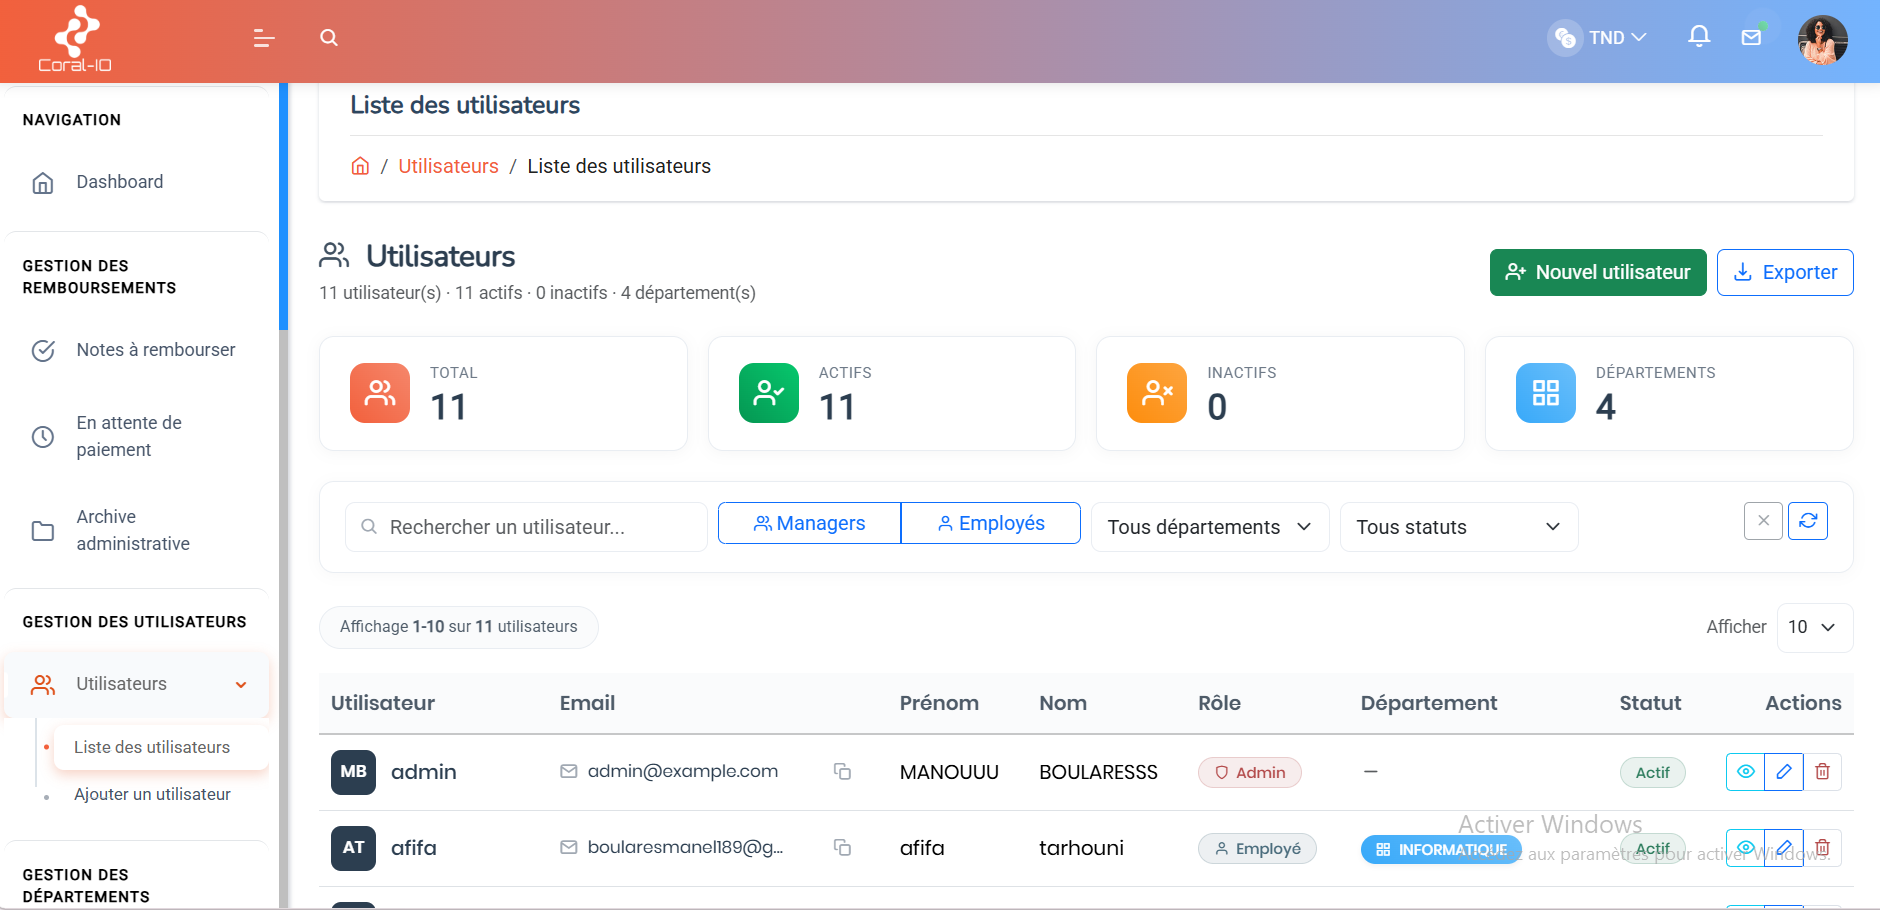
\includegraphics[width=\textwidth]{interface_users_list.png}

 \caption{Interface liste des utilisateurs}

 \label{fig:interface_users_list}

\end{figure}



\subsubsection{Interface d'ajout d'un utilisateur}

L'administrateur accède à cette interface en cliquant sur le bouton "Nouvel utilisateur". Il doit saisir les informations suivantes : nom d'utilisateur, email, mot de passe et confirmation, prénom, nom, rôle (Employé/Manager/Admin), département (optionnel). Il peut également définir le statut du compte (activé/désactivé) et si l'email est vérifié. Un email d'invitation est automatiquement envoyé à l'utilisateur avec ses identifiants. Une modale de confirmation s'affiche avant la création.



\begin{figure}[H]

 \centering

 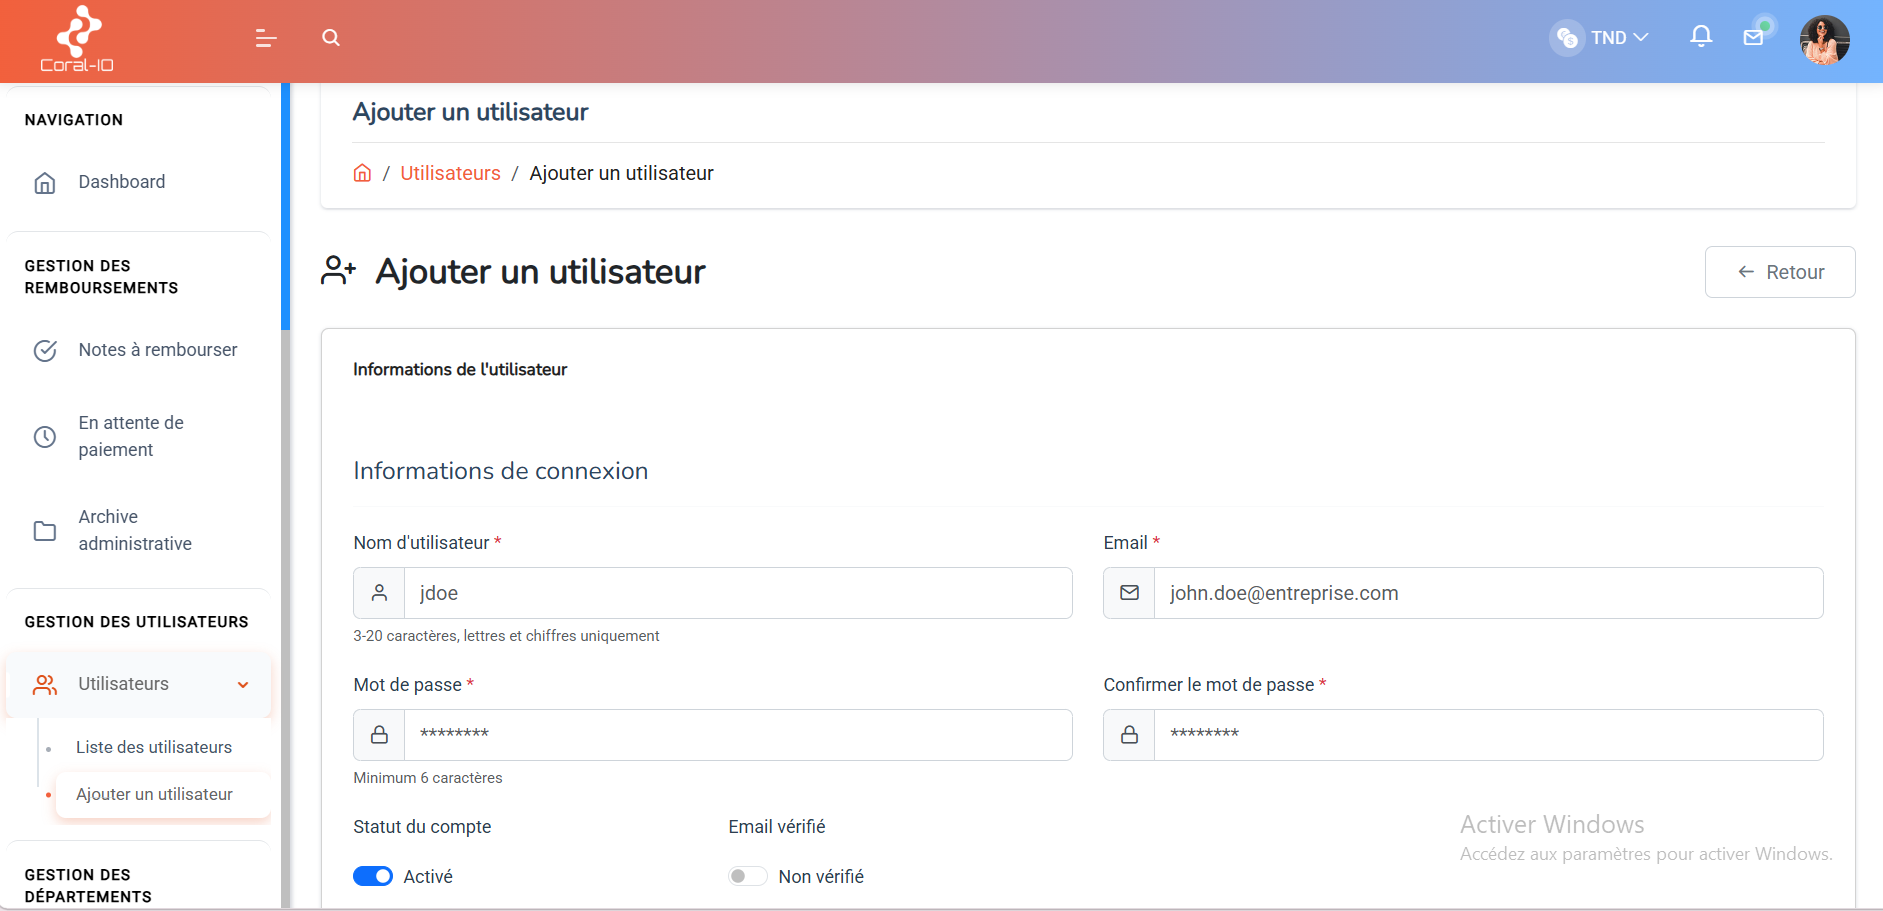
\includegraphics[width=\textwidth]{interface_user_add.png}

 \caption{Interface d'ajout d'utilisateur}

 \label{fig:interface_user_add}

\end{figure}



\subsubsection{Interface de modification d'un utilisateur}

L'administrateur accède à cette interface en cliquant sur le bouton "Modifier" dans la liste des utilisateurs. Les champs sont pré-remplis avec les informations actuelles. Il peut modifier l'email, le prénom, le nom, le rôle, le département, le statut du compte et la vérification de l'email. Le nom d'utilisateur est en lecture seule. Un champ optionnel permet de changer le mot de passe (laissé vide pour le conserver). Les modifications sont enregistrées après validation.



\begin{figure}[H]

 \centering

 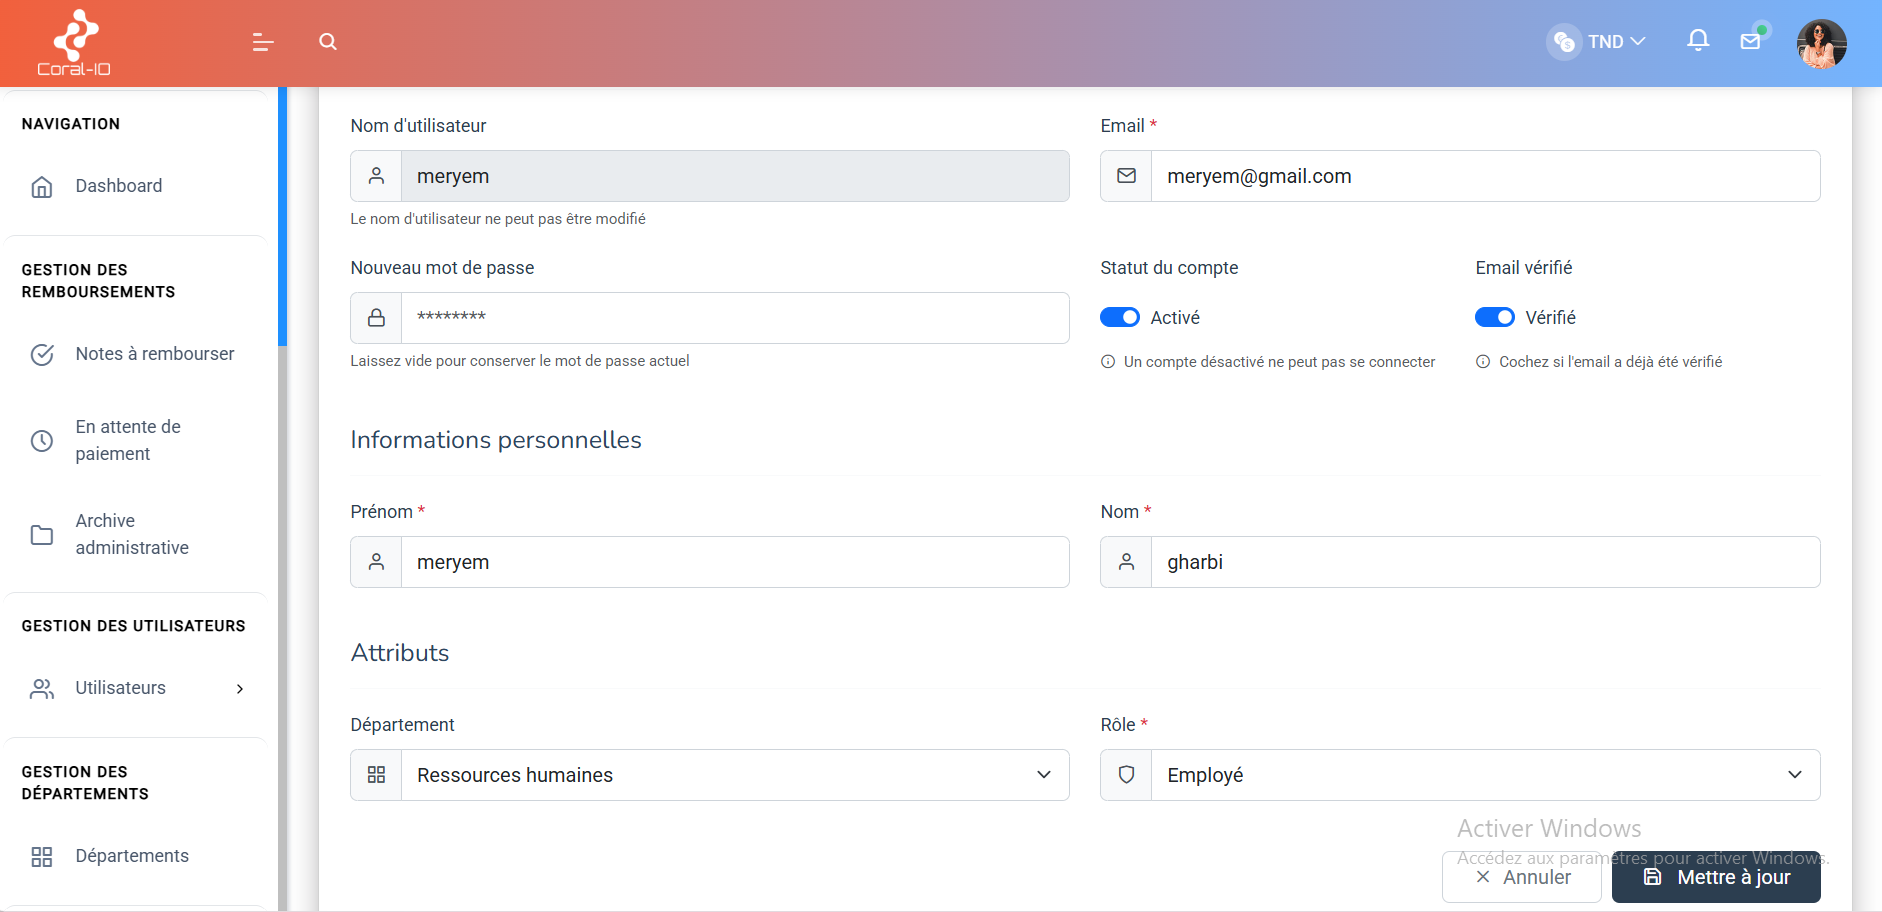
\includegraphics[width=\textwidth]{interface_user_edit.png}

 \caption{Interface de modification d'utilisateur}

 \label{fig:interface_user_edit}

\end{figure}



\subsection{Gestion des profils}



\subsubsection{Interface de consultation du profil}

Chaque utilisateur (Employé, Manager ou Administrateur) peut consulter son profil. L'interface affiche les informations personnelles : nom d'utilisateur, prénom, nom, email, téléphone, localisation et département. Le statut du compte (actif/inactif) et la vérification de l'email sont également affichés. Un avatar avec les initiales de l'utilisateur est présenté. L'utilisateur peut cliquer sur "Modifier" pour accéder au formulaire d'édition ou sur "Changer le mot de passe" pour ouvrir la modale de changement.



\begin{figure}[H]

 \centering

 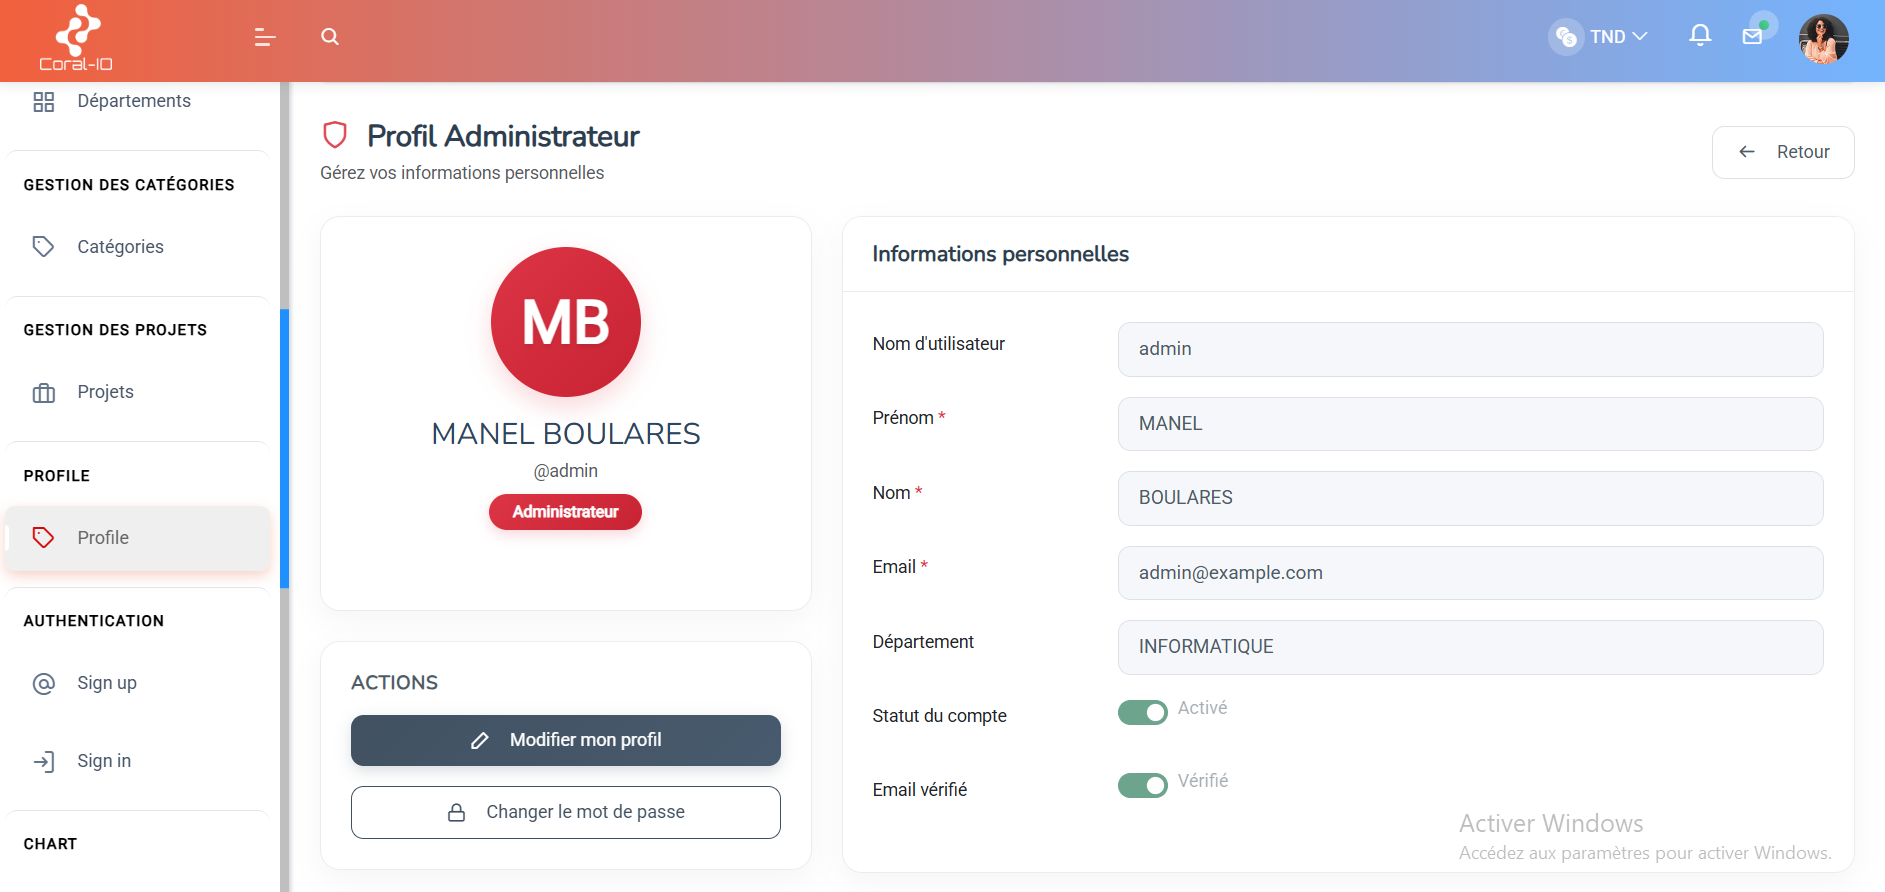
\includegraphics[width=\textwidth]{interface_profile_view.png}

 \caption{Interface de consultation du profil administrateur}

 \label{fig:interface_profile_view}

\end{figure}



\begin{figure}[H]

 \centering

 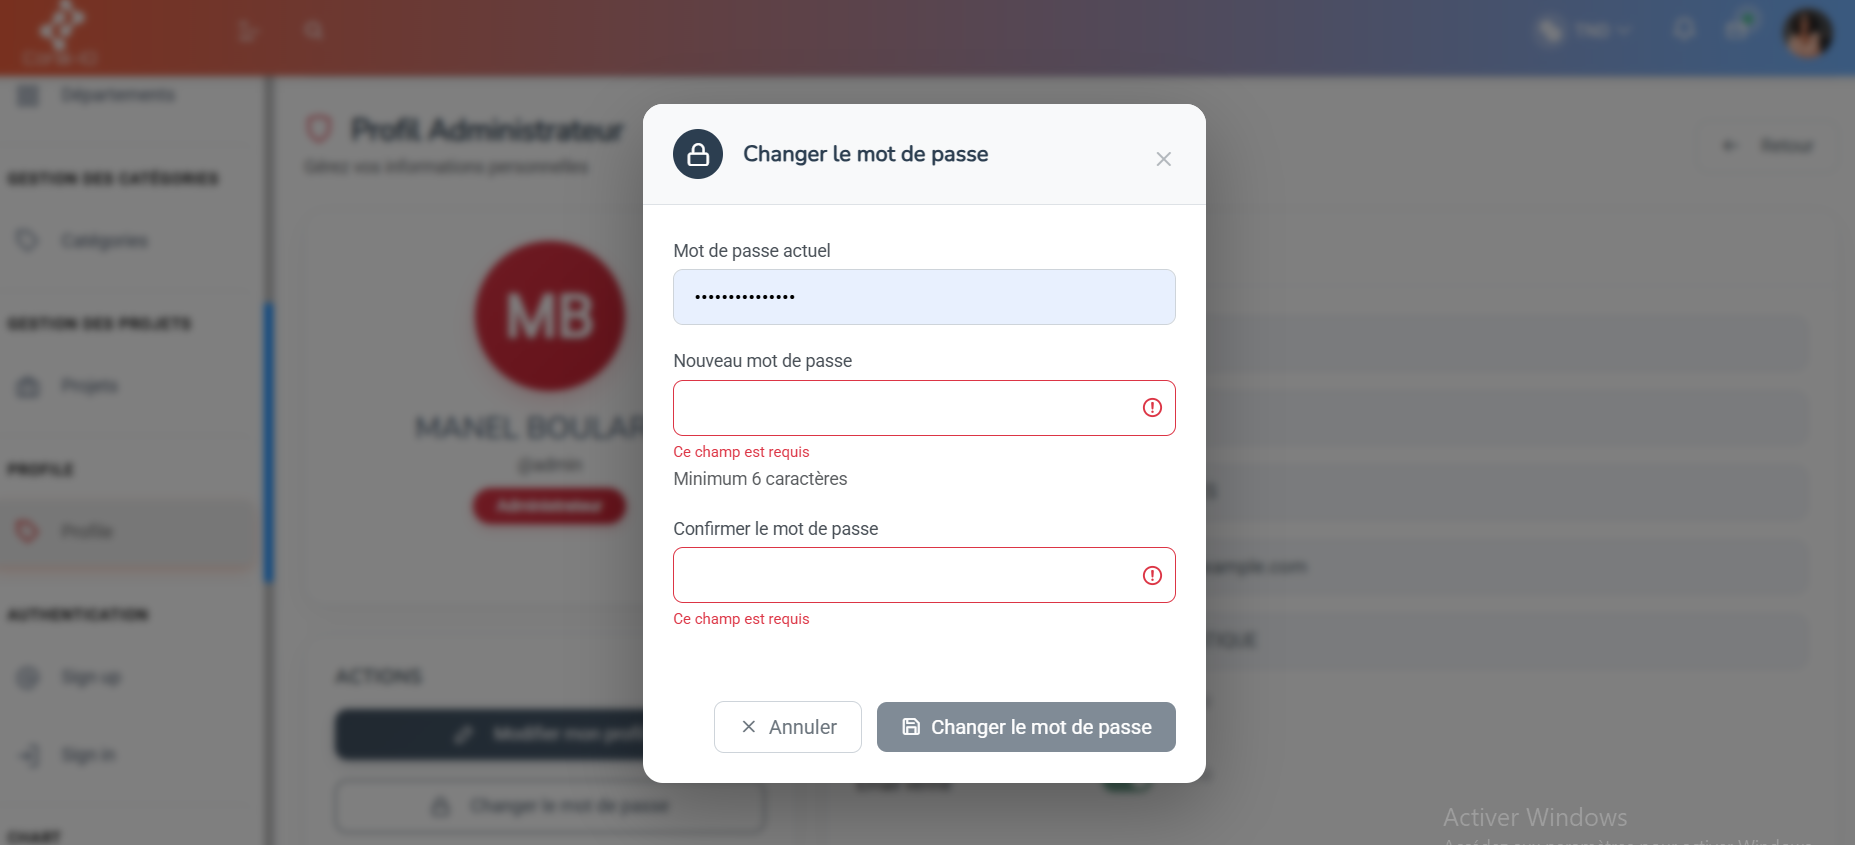
\includegraphics[width=\textwidth]{modal_change_password.png}

 \caption{Modale de changement de mot de passe}

 \label{fig:modal_change_password}

\end{figure}



\subsubsection{Interface de modification du profil}

En mode édition, l'utilisateur peut modifier ses informations personnelles : prénom, nom, téléphone et localisation. L'email n'est pas modifiable (seul l'administrateur peut le changer). Le nom d'utilisateur est également en lecture seule. L'utilisateur clique sur "Enregistrer" pour valider les modifications ou "Annuler" pour revenir à la consultation. Un message de succès ou d'erreur s'affiche après la soumission.



\begin{figure}[H]

 \centering

 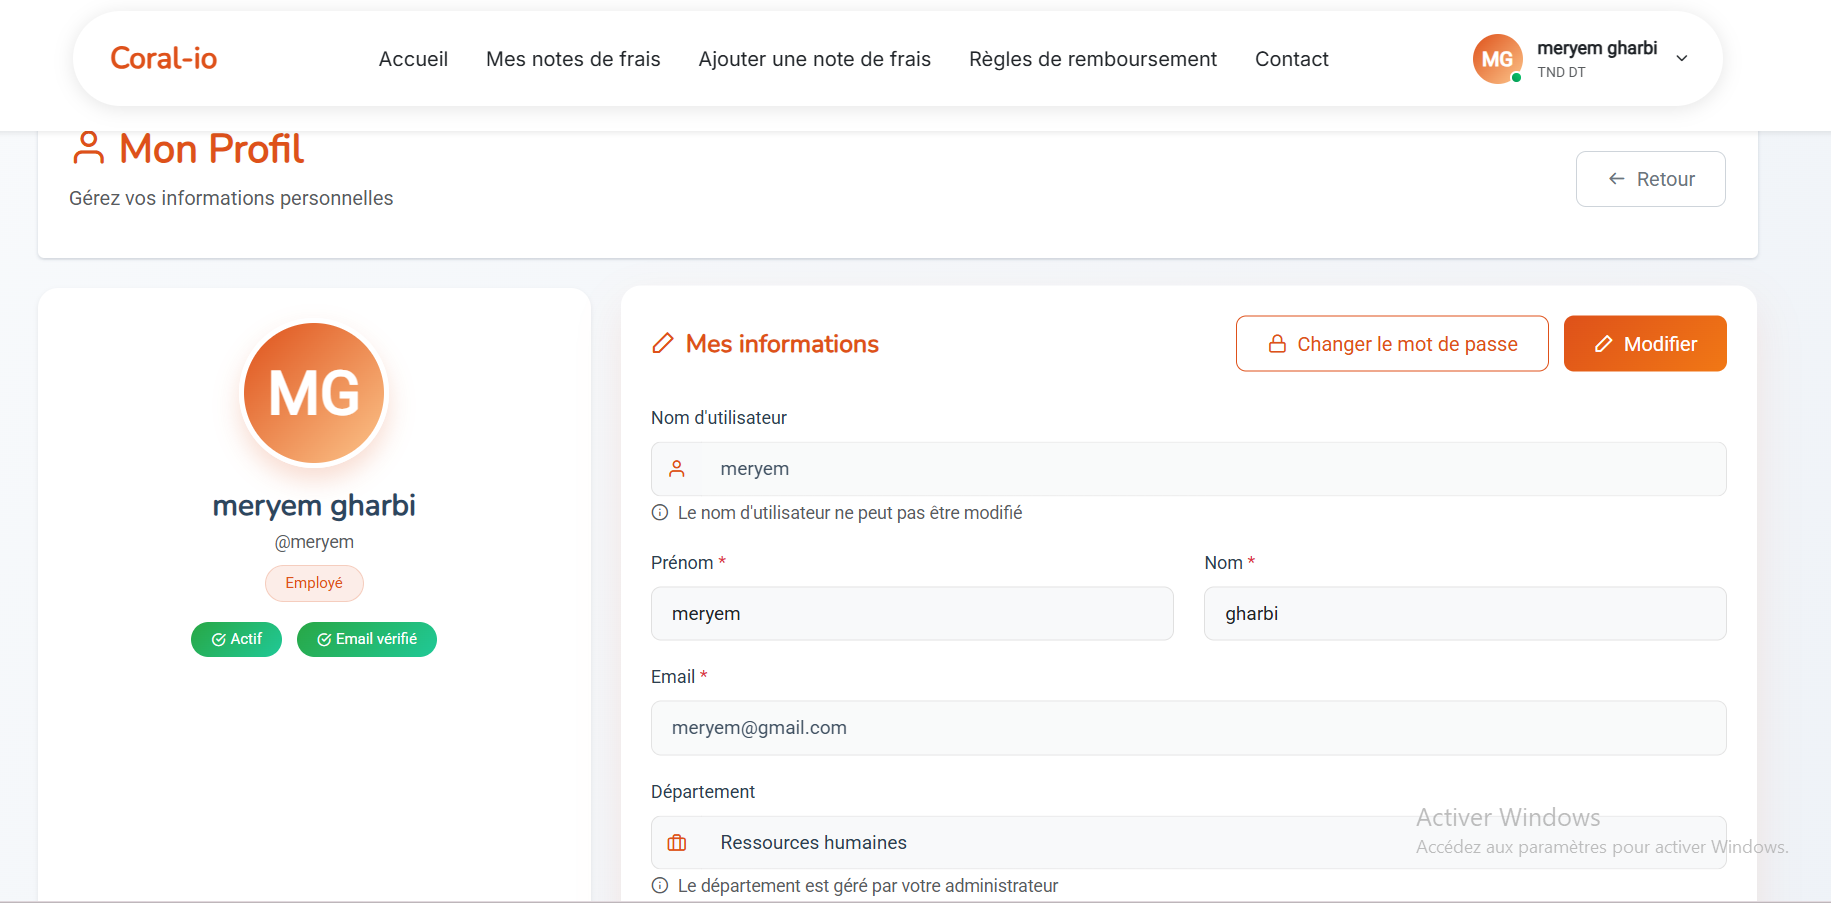
\includegraphics[width=\textwidth]{interface_profile_edit.png}

 \caption{Interface de modification du profil employé}

 \label{fig:interface_profile_edit}

\end{figure}



\begin{figure}[H]

 \centering

 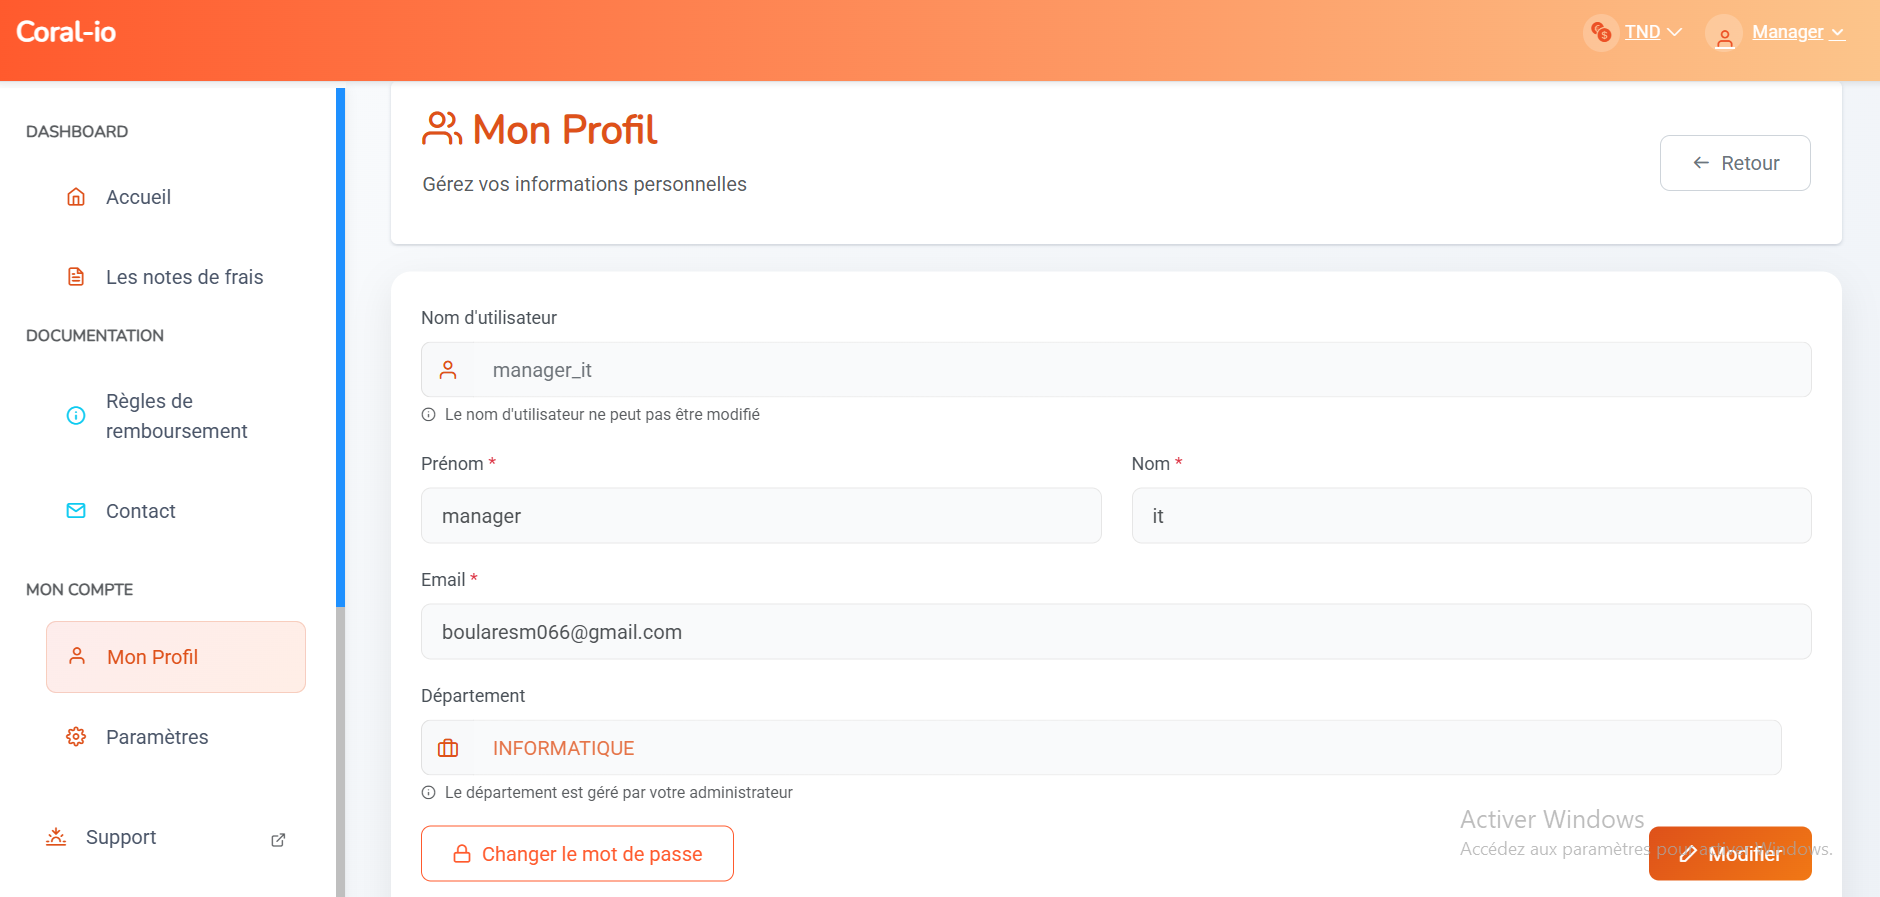
\includegraphics[width=\textwidth]{interface_profile_edit_manager.png}

 \caption{Interface de modification du profil manager}

 \label{fig:interface_profile_edit_manager}

\end{figure}



\subsection{Gestion des départements }



\subsubsection{Interface de liste des départements}

L'administrateur accède à la liste de tous les départements. Cette interface présente des statistiques (total, actifs, inactifs) et permet de rechercher un département par nom. Des filtres par statut (actif/inactif) et par période de création sont disponibles. Chaque département est affiché sous forme de carte avec son code, nom, description, contacts (email, téléphone, localisation), statut et date de création. L'administrateur peut modifier, activer/désactiver ou supprimer un département. Un bouton "Nouveau département" permet d'en créer un.



\begin{figure}[H]

 \centering

 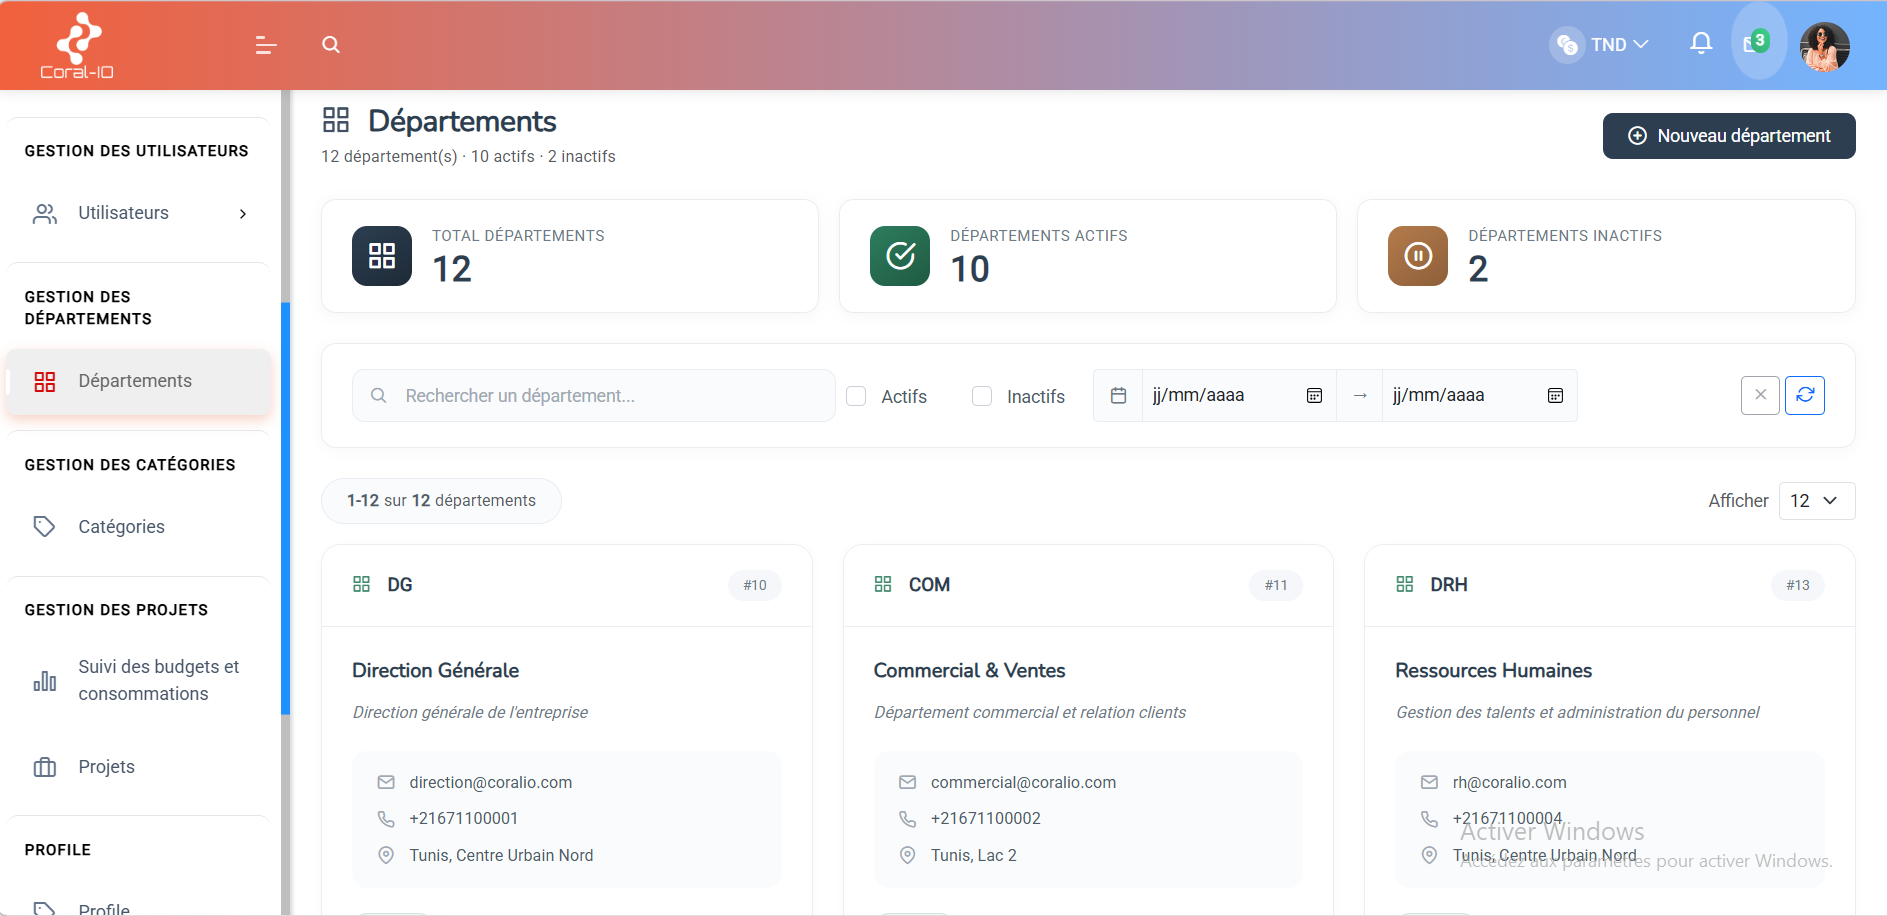
\includegraphics[width=\textwidth]{interface_departments_list.png}

 \caption{Interface liste des départements}

 \label{fig:interface_departments_list}

\end{figure}



\subsubsection{Interface d'ajout/modification d'un département}

L'administrateur saisit les informations du département : nom, code unique, statut (actif/inactif), description, email, téléphone et localisation. En mode modification, les champs sont pré-remplis. La validation côté formulaire garantit le respect des contraintes. L'administrateur clique sur "Créer" ou "Mettre à jour" pour enregistrer.



\begin{figure}[H]

 \centering

 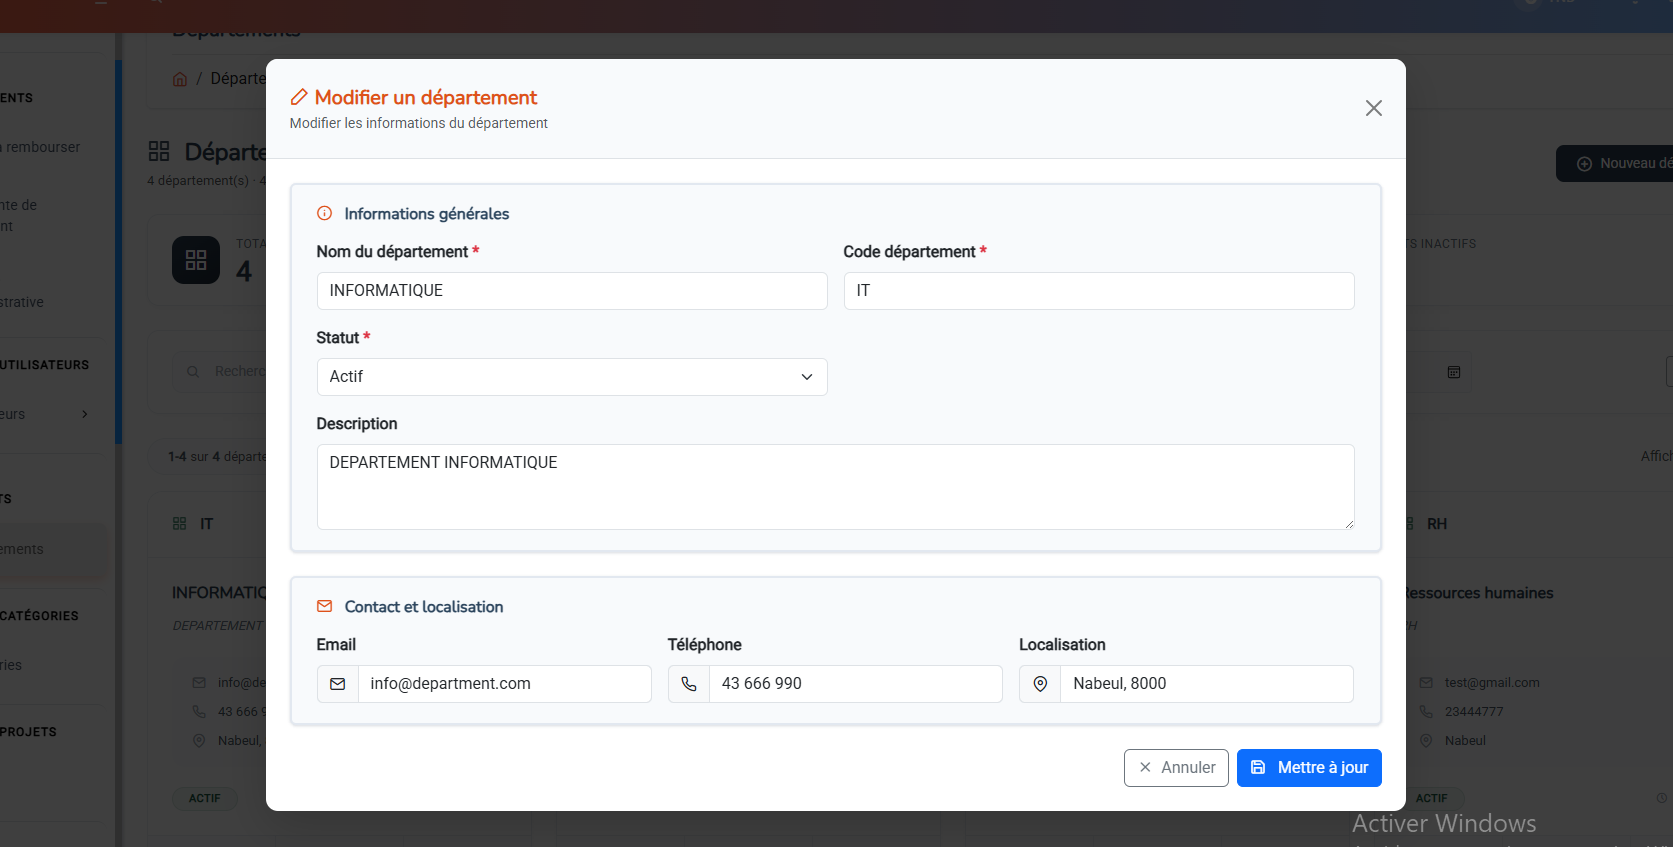
\includegraphics[width=\textwidth]{interface_department_form.png}

 \caption{Interface d'ajout/modification de département}

 \label{fig:interface_department_form}

\end{figure}



\subsection{Gestion des projets }



\subsubsection{Interface de liste des projets}

L'administrateur visualise tous les projets sous forme de cartes, avec des statistiques résumant le total des projets, ceux en cours, inactifs, clôturés et le budget total. Des filtres permettent de rechercher par nom, statut (actif/inactif/clôturé) et période. Chaque carte affiche le code, le nom, la description, le département associé, le budget, les dates de début et fin, le statut et la date de création. L'administrateur peut voir les employés assignés, modifier le projet, son statut, ou le supprimer. Un bouton « Nouveau projet » permet d'accéder au formulaire de création.



\begin{figure}[H]

 \centering

 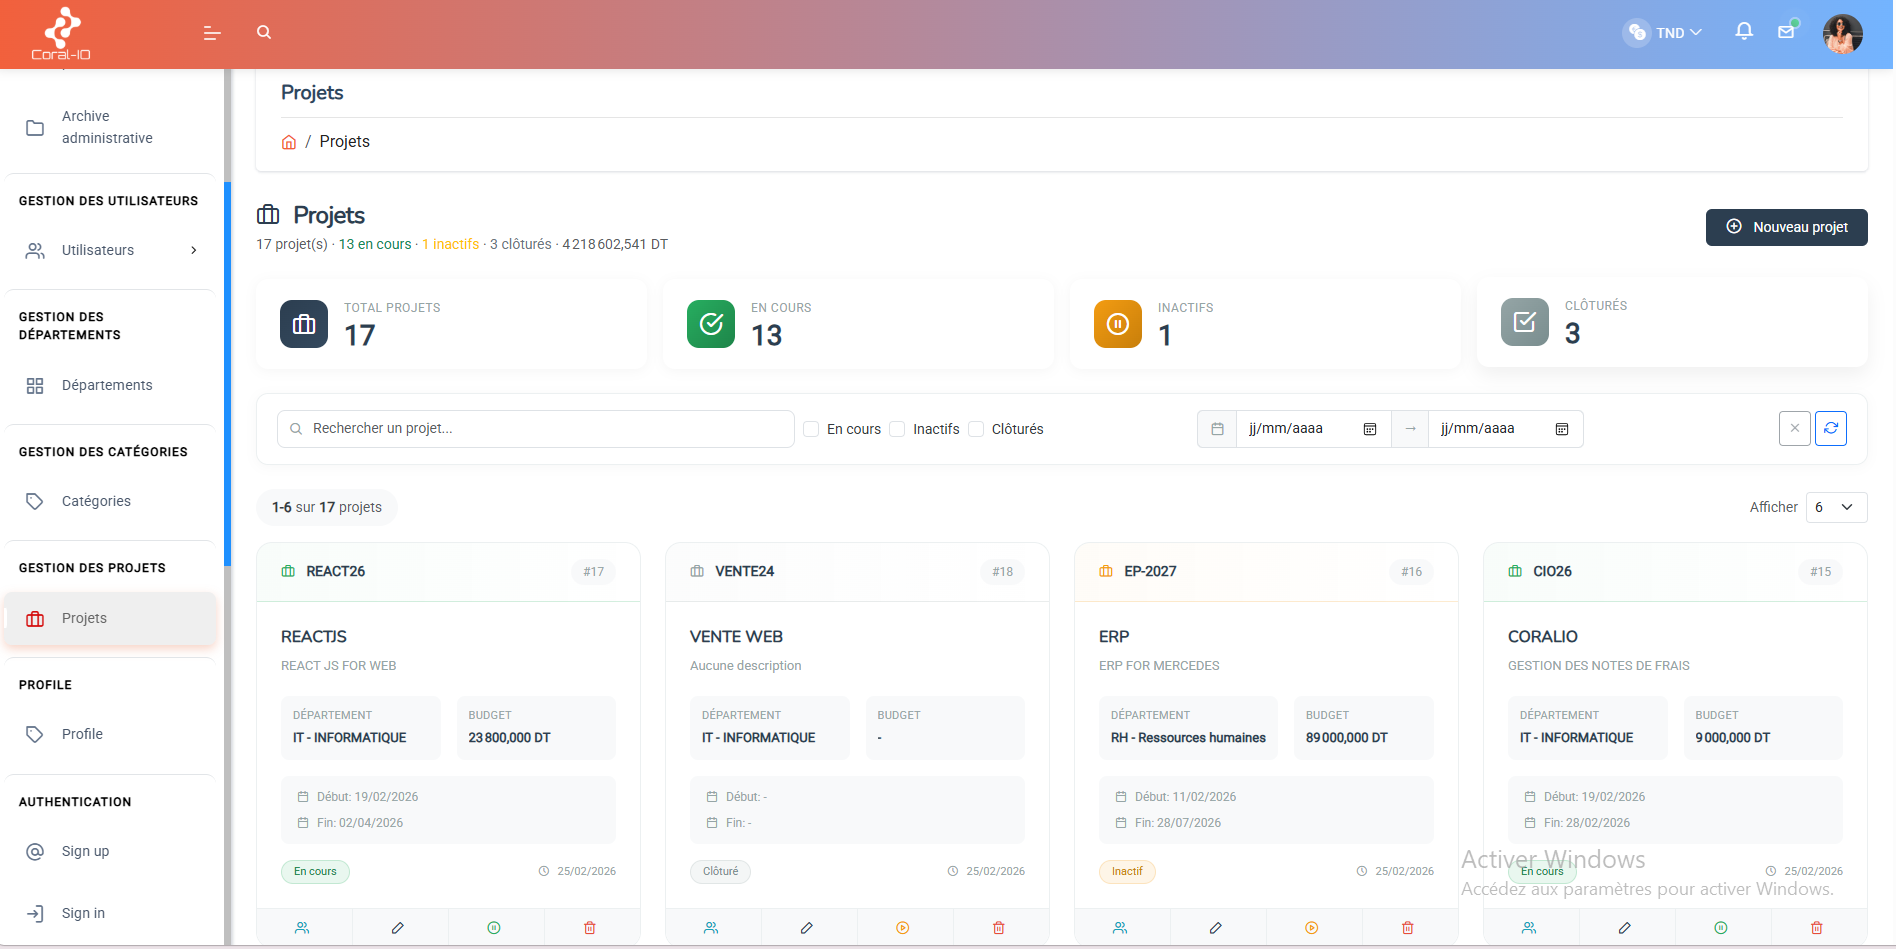
\includegraphics[width=\textwidth]{interface_projects_list.png}

 \caption{Interface liste des projets}

 \label{fig:interface_projects_list}

\end{figure}



\subsubsection{Interface d'ajout/modification d'un projet}

L'administrateur saisit les informations du projet : nom, code unique, département, statut, description, budget, dates de début et fin, et sélectionne les employés à affecter au projet. Une barre de recherche permet de filtrer les employés par nom ou email. L'administrateur peut sélectionner/désélectionner tous les employés ou individuellement. La validation garantit que le nom et le code sont uniques. Le budget peut être saisi dans différentes devises (conversion automatique en TND).



\begin{figure}[H]

 \centering

 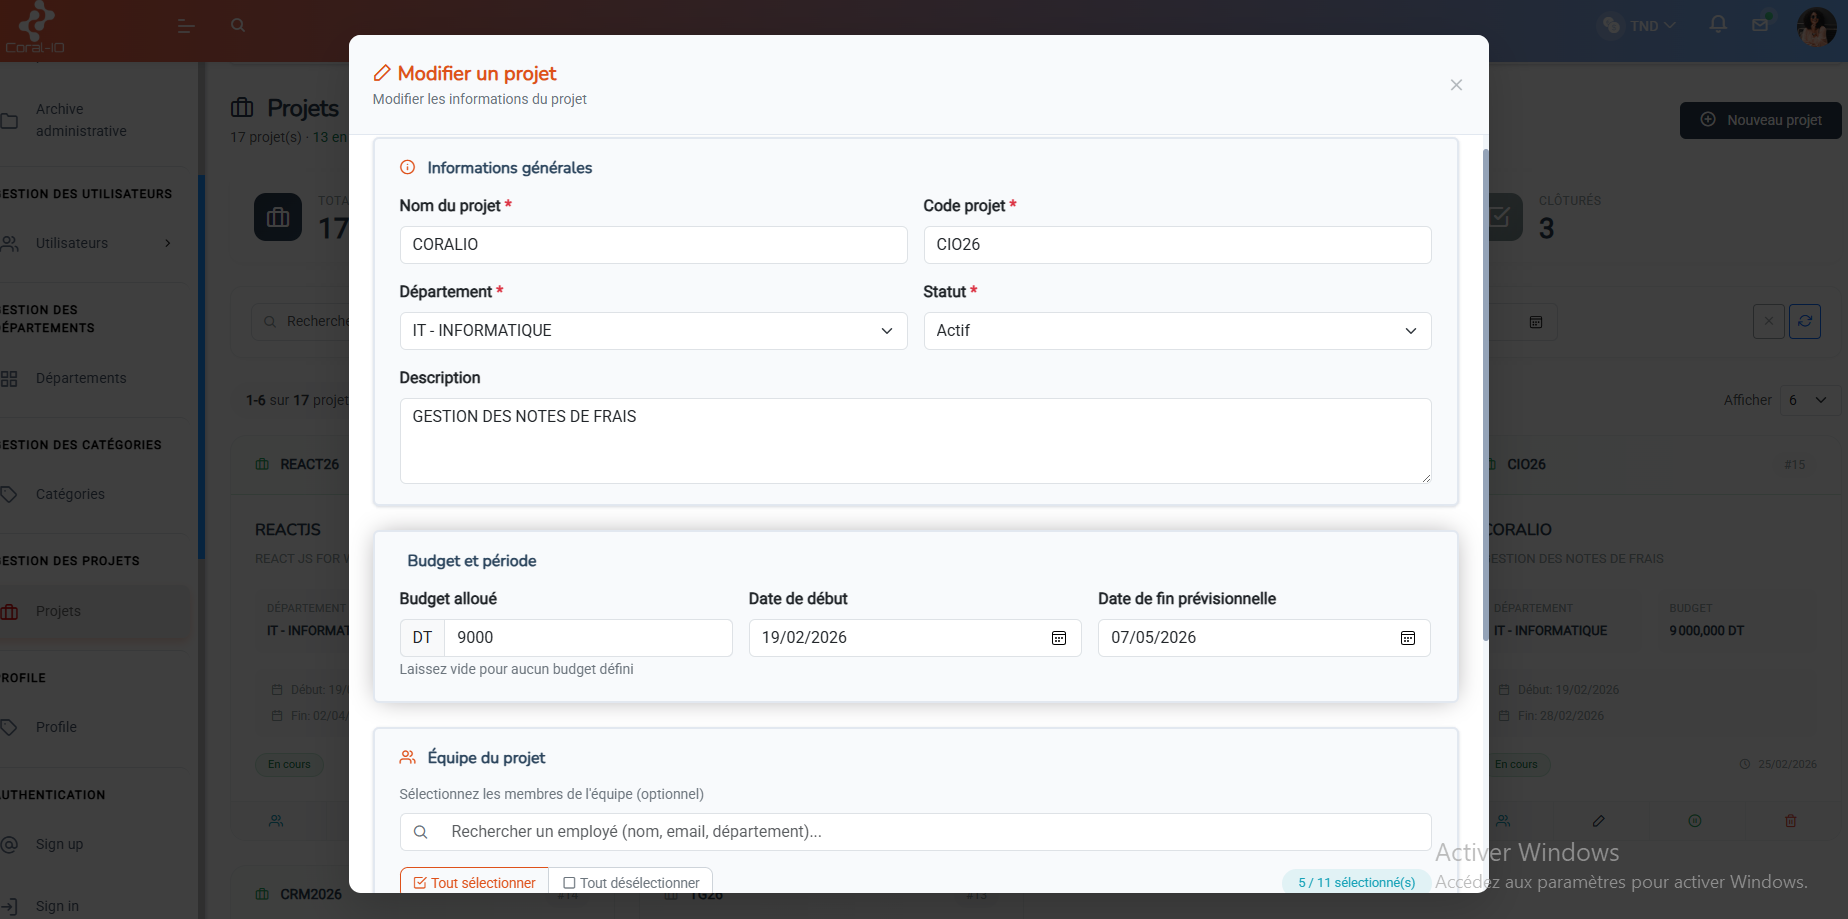
\includegraphics[width=\textwidth]{interface_project_form.png}

 \caption{Interface d'ajout/modification de projet}

 \label{fig:interface_project_form}

\end{figure}



\subsubsection{Interface de consultation des projets (pour employé)}

L'employé peut consulter ses projets, leurs délais et la répartition de ses notes sur ces projets.



\begin{figure}[H]

 \centering

 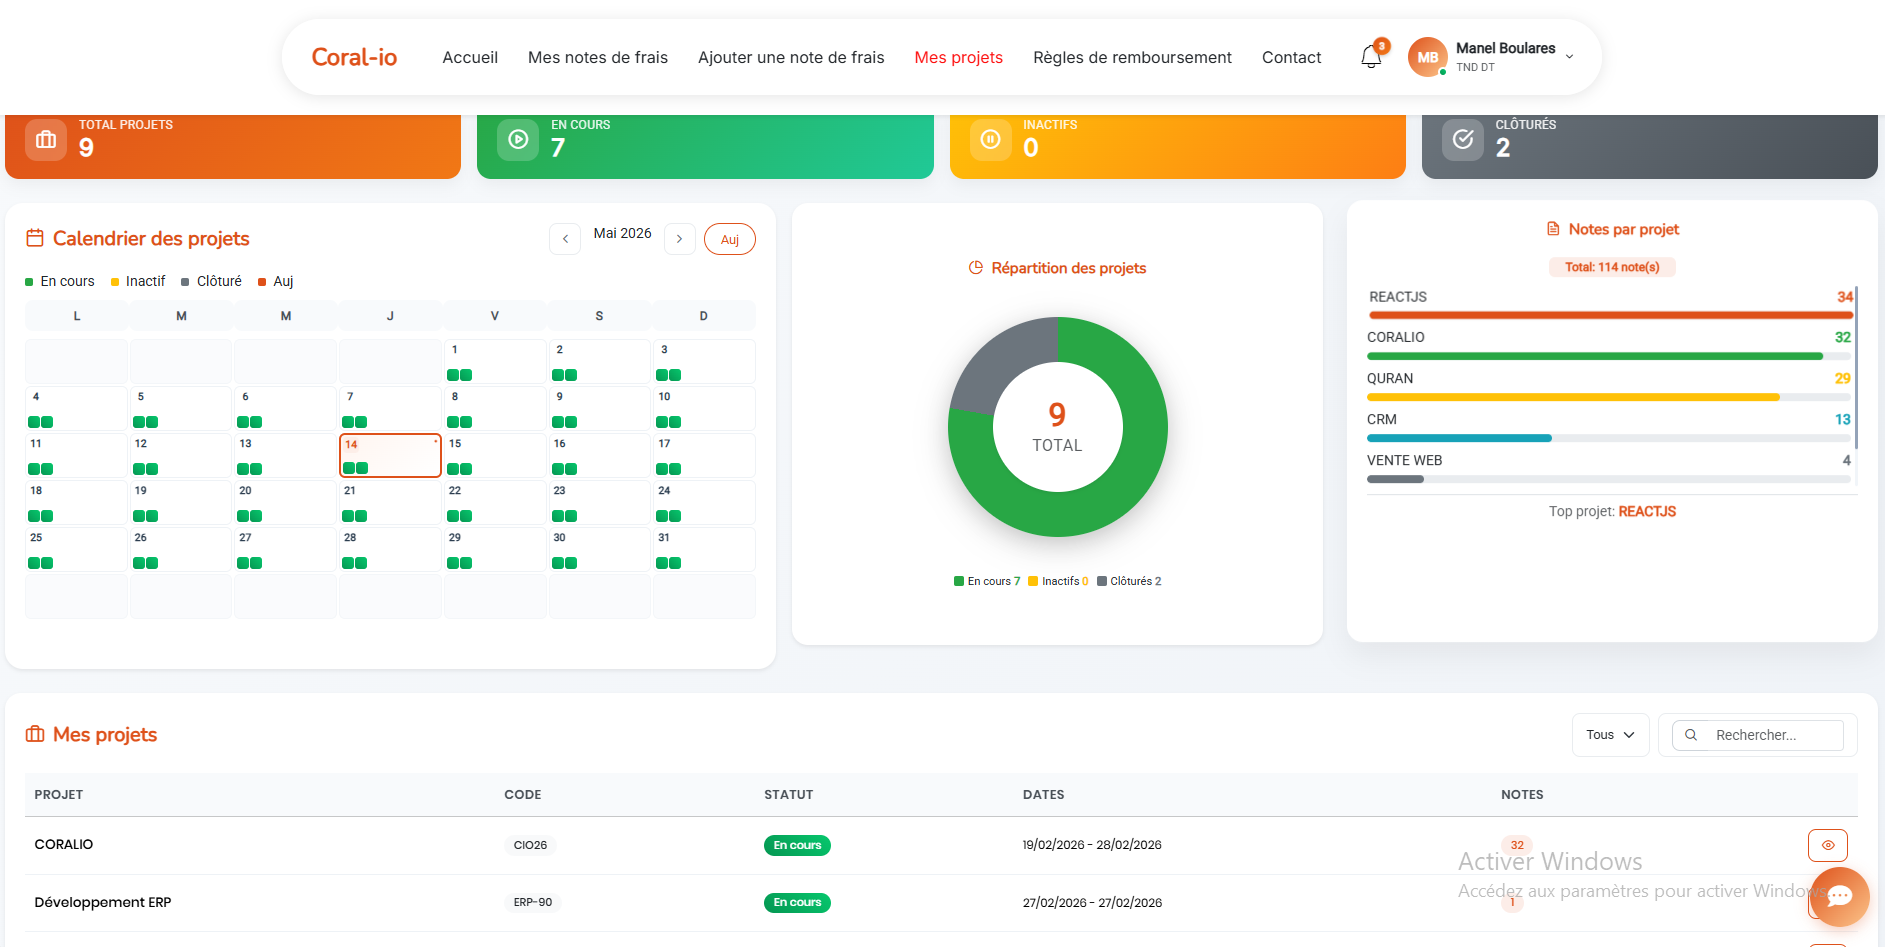
\includegraphics[width=\textwidth]{my-projects.png}

 \caption{Interface de consultation des projets }

 \label{fig:mes_projets}

\end{figure}



\subsubsection{Interface de consultation des régles de remboursement}

L'employé peut consulter les régles de remboursement, notamment les catégories disponibles et leurs plafonds.



\begin{figure}[H]

 \centering

 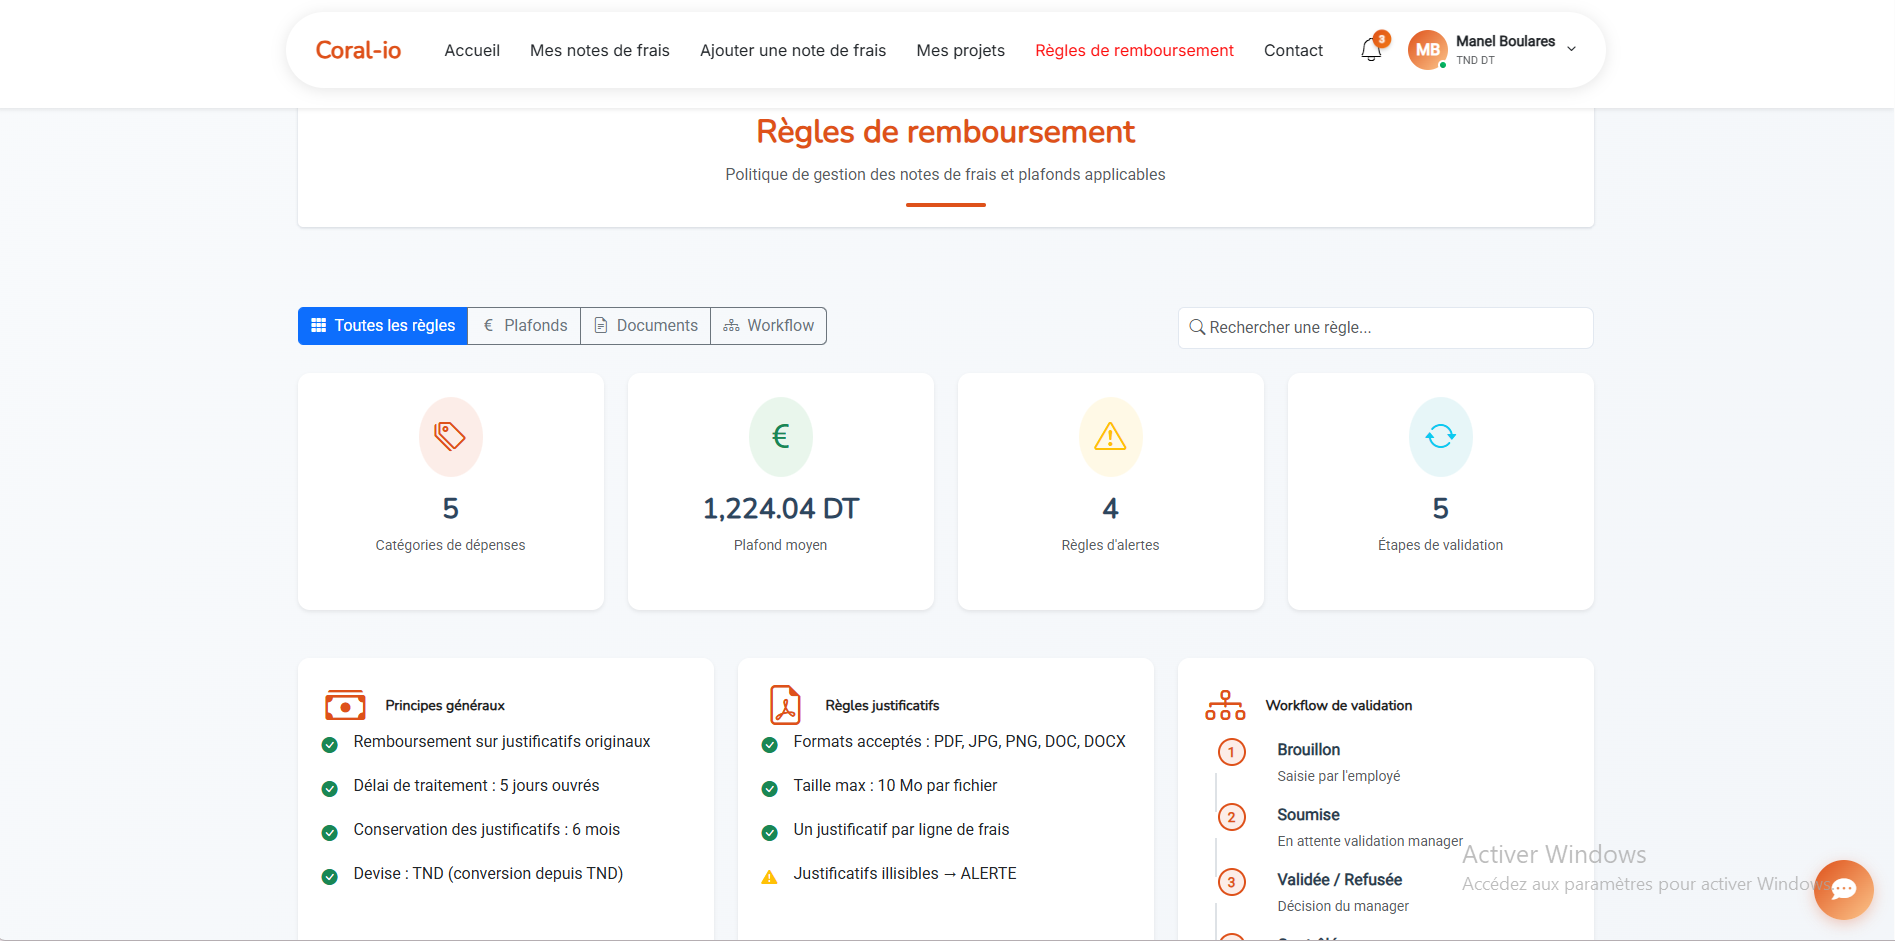
\includegraphics[width=\textwidth]{regles-remboursement.png}

 \caption{Interface de consultation des régles de remboursement}

 \label{fig:regles_remboursement}

\end{figure}





\subsection{Gestion des catégories de dépenses}



\subsubsection{Interface de liste des catégories}

L'administrateur visualise toutes les catégories de dépenses sous forme de cartes. Des statistiques présentent le total des catégories, actives et inactives. Des filtres permettent de rechercher par nom, par statut et par plafond (mini/maxi). Chaque carte affiche le nom, la description, le plafond, le nombre de champs associés, le nombre de champs requis et le statut. L'administrateur peut modifier, activer/désactiver ou supprimer une catégorie. Un bouton "Nouvelle catégorie" permet d'en créer une.



\begin{figure}[H]

 \centering

 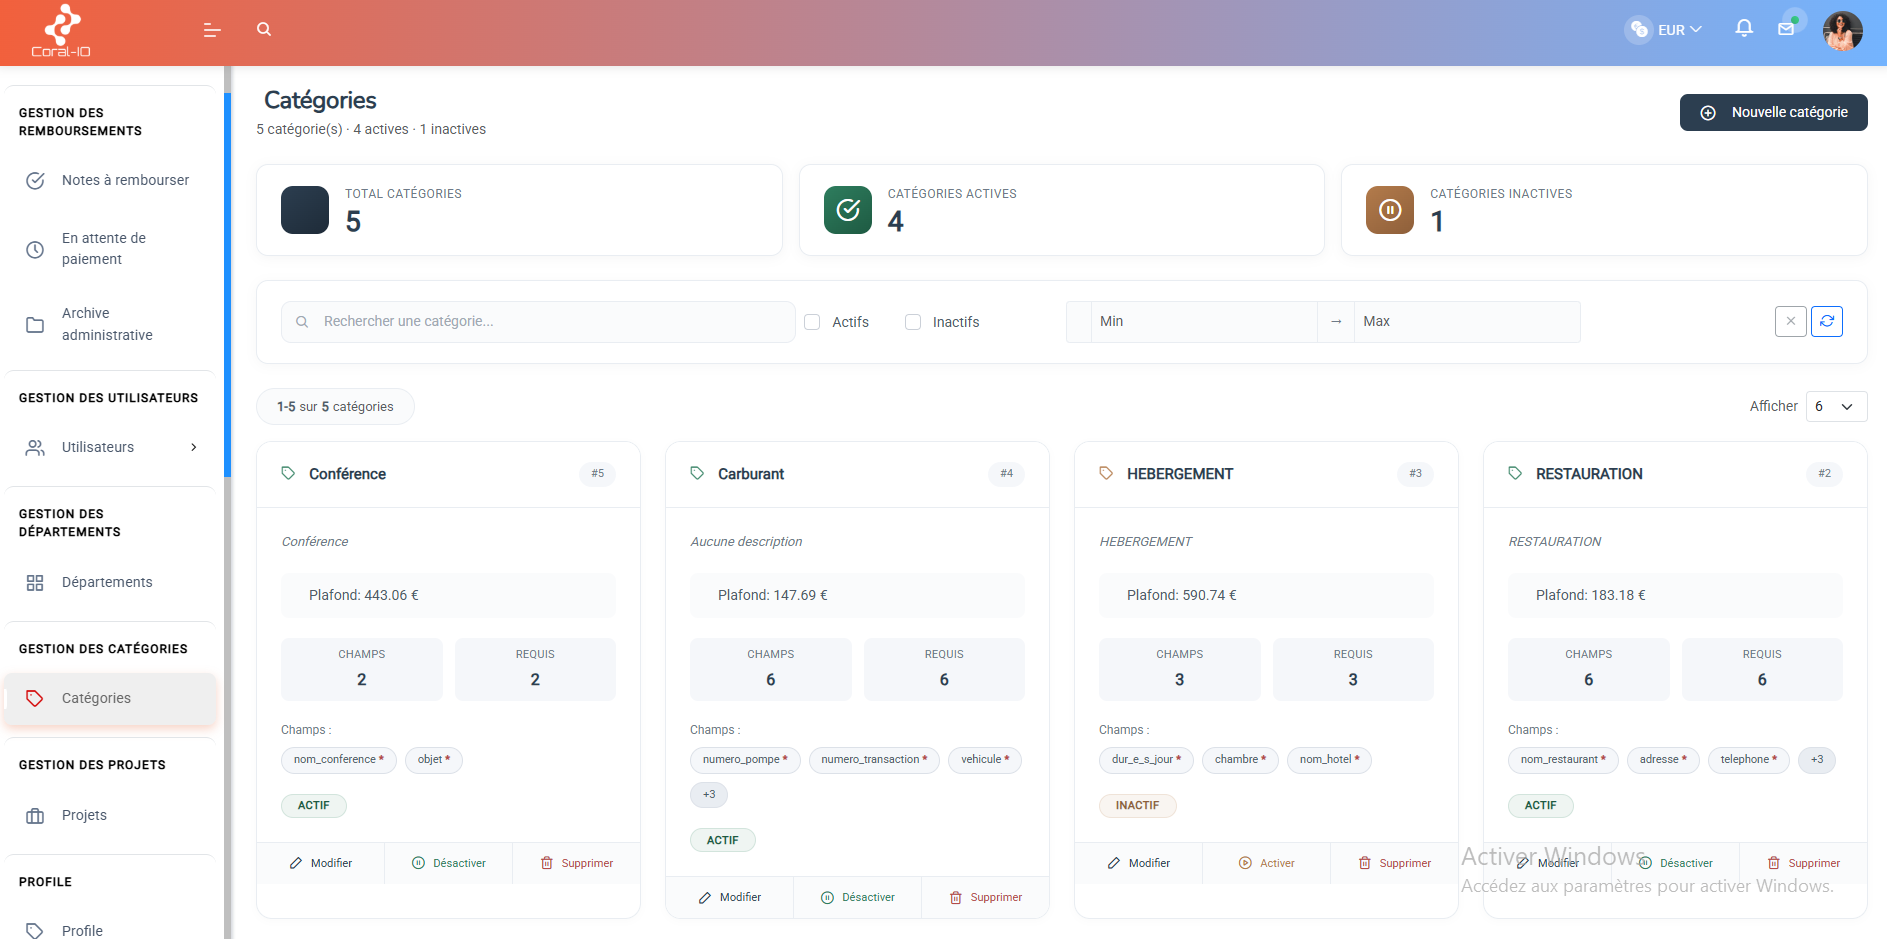
\includegraphics[width=\textwidth]{interface_categories_list.png}

 \caption{Interface liste des catégories}

 \label{fig:interface_categories_list}

\end{figure}



\subsubsection{Interface d'ajout/modification d'une catégorie avec champs dynamiques}

Cette interface permet à l'administrateur de créer ou modifier une catégorie de dépenses avec des champs personnalisés dynamiques. Il saisit le nom, le plafond (optionnel), la description et le statut, puis ajoute des champs personnalisés (nom, type, requis), sélectionne des champs courants, parcourt la bibliothèque des colonnes existantes ou organise l'ordre des champs. Les champs existants sont affichés avec un badge « EXISTANT », tandis que les nouveaux déclenchent la création automatique de colonnes. L'administrateur peut sélectionner plusieurs champs à la fois et les ajouter en bloc via une barre de recherche.



\begin{figure}[H]

 \centering

 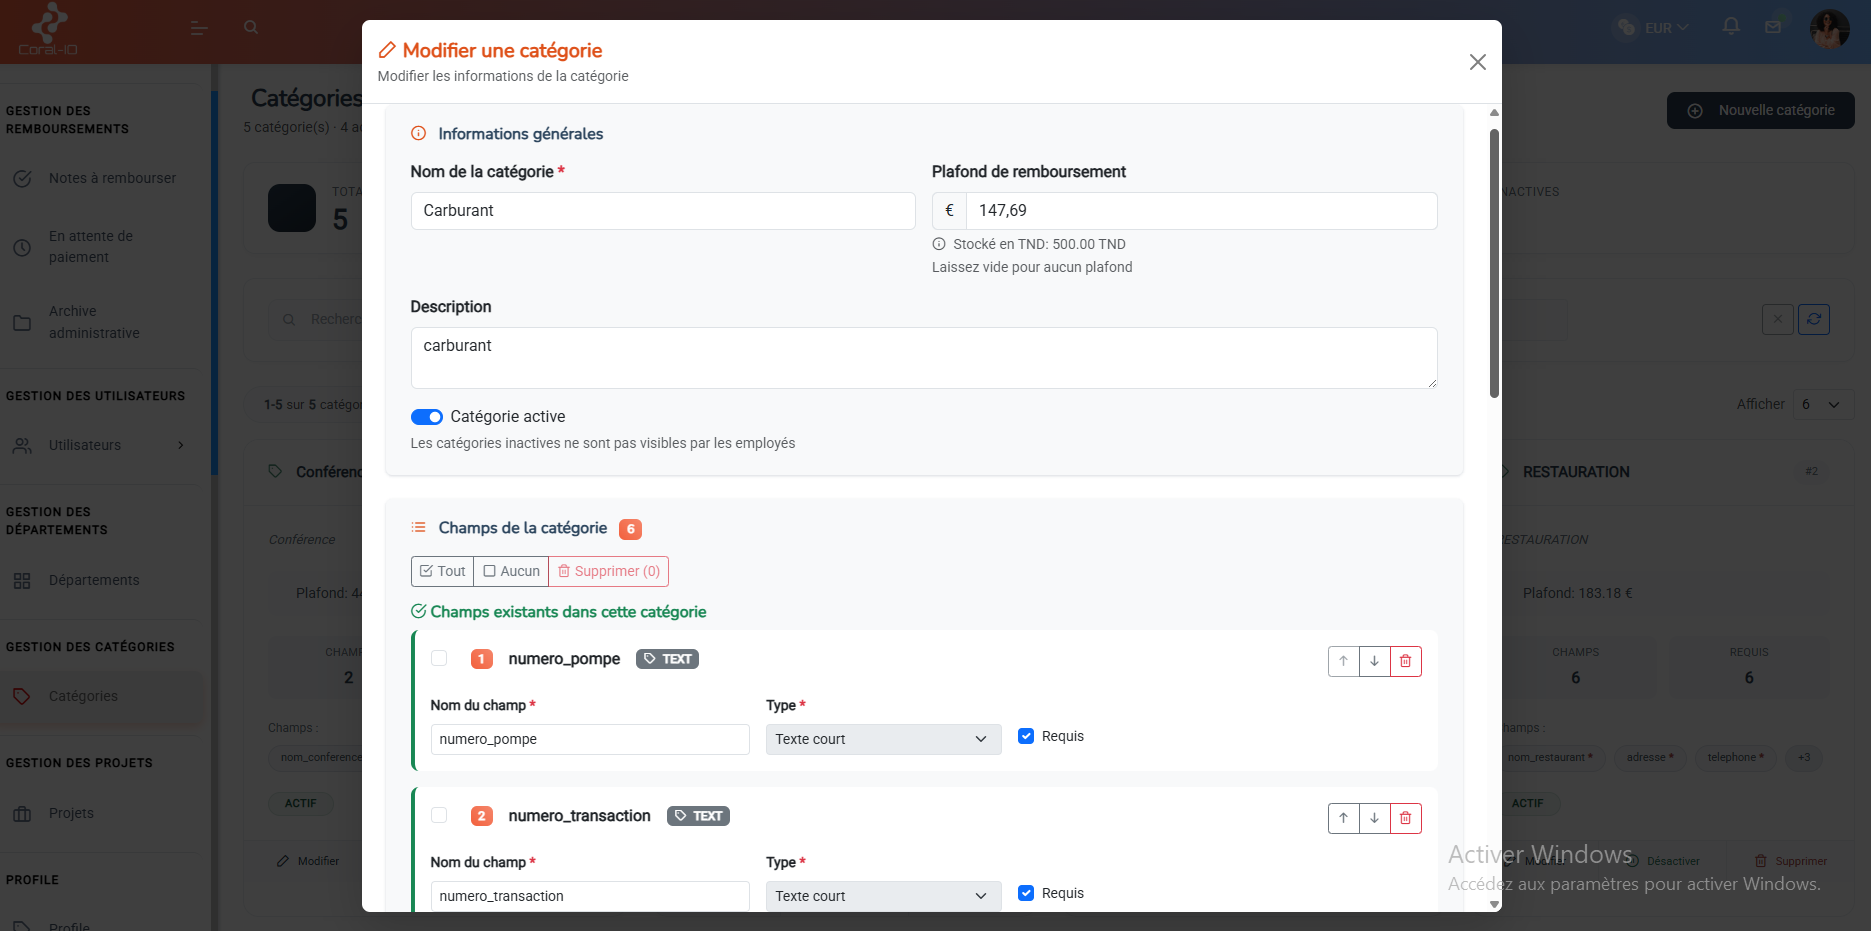
\includegraphics[width=\textwidth]{interface_category_form.png}

 \caption{Interface d'ajout/modification de catégorie }

 \label{fig:interface_category_form}

\end{figure}



\begin{figure}[H]

 \centering

 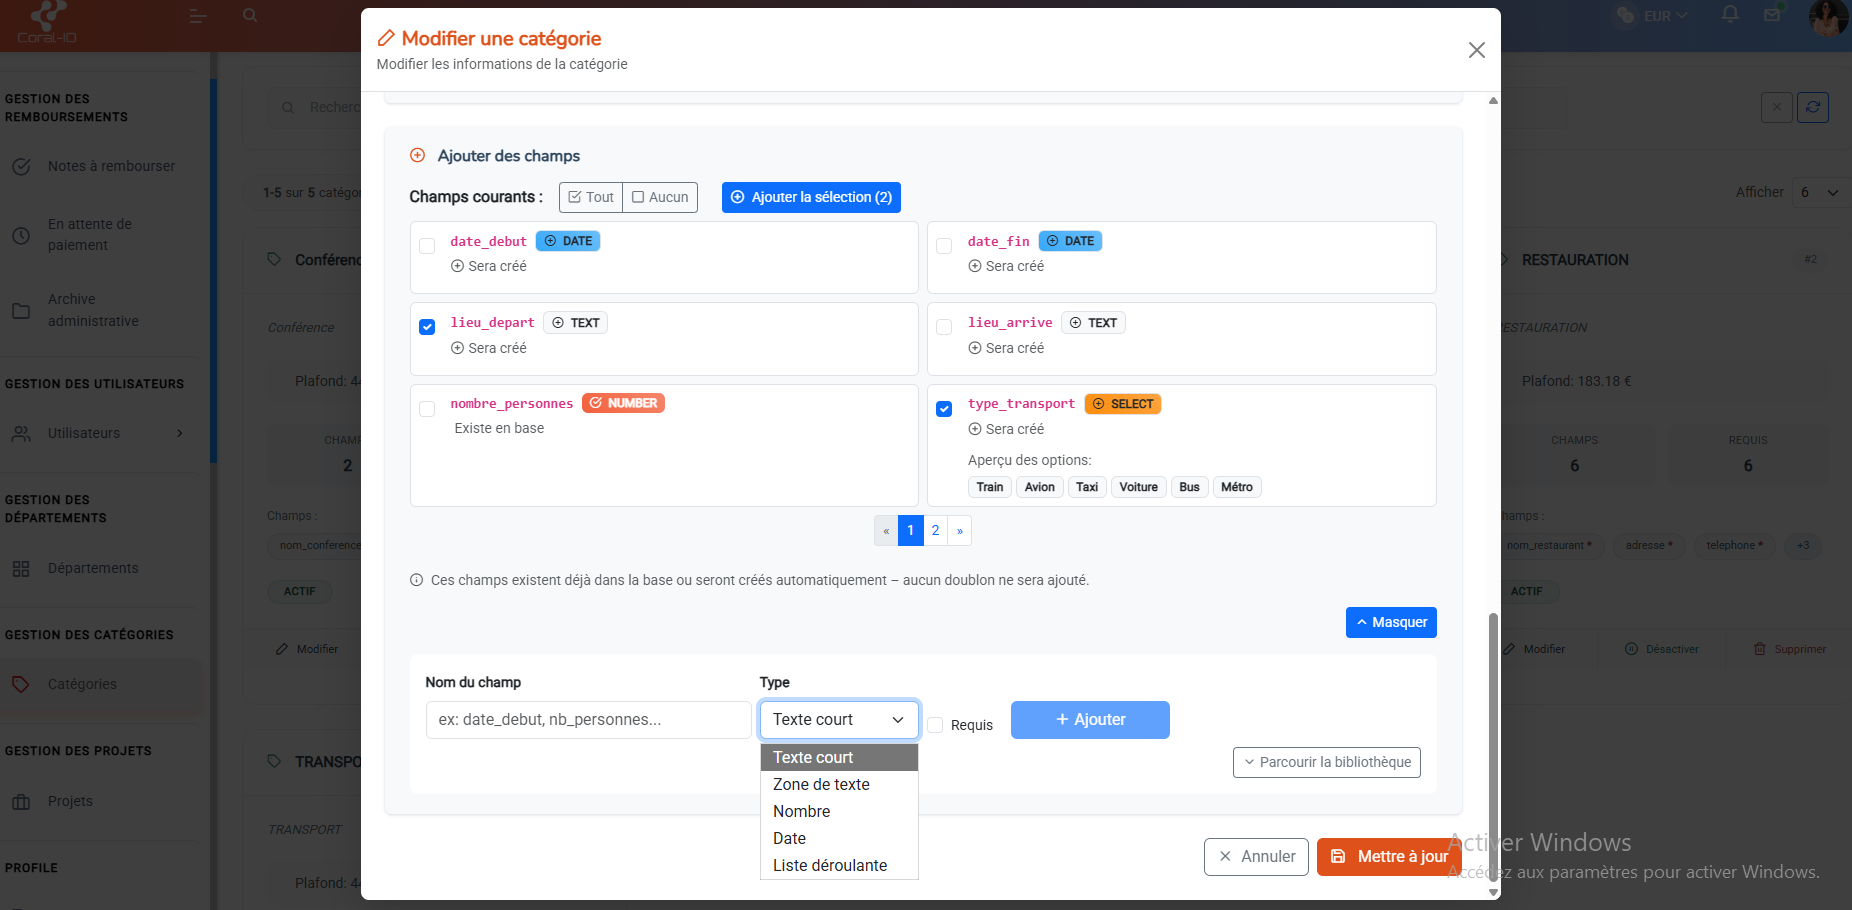
\includegraphics[width=\textwidth]{interface_category_form_fields.png}

 \caption{Interface de gestion des champs des catégories}

 \label{fig:interface_category_form_fields}

\end{figure}



\textbf{Fonctionnalités :}

\begin{itemize}

 \item Liste des catégories existantes

 \item Création d'une nouvelle catégorie (nom, plafond)

 \item Ajout de champs personnalisés (texte, nombre, date, booléen, liste déroulante)

 \item Modification/suppression de catégories

 \item Visualisation des champs associés à chaque catégorie

\end{itemize}

\section*{Conclusion}

\addcontentsline{toc}{section}{Conclusion}

Dans ce sprint, nous avons mis en place les fondations de Coral.io : la gestion des utilisateurs avec Keycloak, l'authentification JWT, la récupération de mot de passe, ainsi que la gestion des départements, projets et catégories avec champs personnalisés dynamiques. Ces bases nous permettent d'aborder le sprint suivant dédié à la création et gestion des notes de frais.

\newpage



\chapter{Sprint 2 « Gestion des notes de frais »}



\section*{Introduction}

\addcontentsline{toc}{section}{Introduction}

Ce chapitre présente le Sprint 2 dédié à la « Gestion des notes de frais». Nous détaillerons le Backlog du sprint, le diagramme de cas d'utilisation, les étapes de conception et les interfaces développées.



\section{Objectif du sprint}

L'objectif de ce sprint est de mettre en place un système complet de gestion des notes de frais, incluant la création, la soumission, la modification, la suppression et la consultation des notes et la validation ou le refus par le manager.



\section{Backlog du sprint 2}

Le tableau ci-dessous illustre la décomposition du sprint 2. La durée totale du sprint 2 est de 20 jours ouvrables (du 03/03 au 30/03).



\captionof{table}{Backlog Sprint 2 }

\label{tab:sprint2_combined}

\begin{longtable}{|c|p{5cm}|p{5.5cm}|c|}

\hline

\textbf{ID} & \textbf{User Story} & \textbf{Tâches techniques} & \textbf{Durée (jours)} \\

\hline

\endfirsthead



\hline

\textbf{ID} & \textbf{User Story} & \textbf{Tâches techniques} & \textbf{Durée (jours)} \\

\hline

\endhead



\hline

\multicolumn{4}{|c|}{\textit{Suite dans la page suivante}} \\

\hline

\endfoot



\hline

\endlastfoot



US-32 & En tant qu’employé, je veux créer une note de frais afin de soumettre mes dépenses professionnelles au remboursement. & 

\begin{tabular}[t]{@{}p{5.5cm}@{}}

- Backend: endpoints CRUD notes de frais, soumission, gestion fichiers \\

- Frontend: formulaire de création/édition (champs dynamiques) \\

- Tests unitaires et d’intégration

\end{tabular} & 2j \\

\hline

US-33 & En tant qu’utilisateur, je veux sélectionner une devise (TND/EUR/USD) afin de déclarer ou visualiser des frais dans différentes monnaies. & 

\begin{tabular}[t]{@{}p{5.5cm}@{}}

- Service de taux de change avec API externe et cache local \\

- Frontend: sélecteur de devise et conversion automatique \\

- Tests

\end{tabular} & 1j \\

\hline

US-34 & En tant qu’employé, je veux consulter ma liste de notes avec filtres et pagination afin de retrouver facilement une note passée. & 

\begin{tabular}[t]{@{}p{5.5cm}@{}}

- Frontend: page « Mes notes » (employé) avec tableau, filtres, pagination, détails \\

- Backend: endpoints de récupération des notes par employé \\

- Tests

\end{tabular} & 1j \\

\hline

US-35 & En tant qu’employé, je veux modifier ou supprimer une note en attente afin de corriger des erreurs avant soumission. & 

\begin{tabular}[t]{@{}p{5.5cm}@{}}

- Backend: endpoints modification et suppression \\

- Frontend: édition note et suppression avec confirmation \\

- Tests

\end{tabular} & 1j \\

\hline

US-36 & En tant qu’employé, je veux recevoir des notifications in-app et par email lorsque ma note est validée ou refusée par le manager afin de suivre son état. & 

\begin{tabular}[t]{@{}p{5.5cm}@{}}

- Microservice de notifications (Spring Boot) : envoi d’emails \\

- Frontend: réception et affichage des notifications \\

- Intégration des notifications in-app

\end{tabular} & 2j \\

\hline

US-37 & En tant que manager, je veux lister et filtrer les notes afin d'analyser efficacement les notes de mon département. & 

\begin{tabular}[t]{@{}p{5.5cm}@{}}

- Backend: endpoints pour manager (lister notes du département) \\

- Frontend: page « Demandes à valider » avec tableau, filtres \\

- Tests

\end{tabular} & 2j \\

\hline

US-38 & En tant que manager, je veux recevoir des notifications in-app et par email lorsqu’une nouvelle note est soumise dans un projet de mon département afin de la traiter rapidement. & 

\begin{tabular}[t]{@{}p{5.5cm}@{}}

- Extension du microservice de notifications \\

- Frontend: panneau de notifications, marquage lu/non lu \\

- Tests

\end{tabular} & 1j \\

\hline

US-39 & En tant qu'administrateur, je veux recevoir des notifications in-app et par email lorsqu'une note est validée par le manager avec son commentaire afin de procéder au remboursement. & 

\begin{tabular}[t]{@{}p{5.5cm}@{}}

- Extension du microservice de notifications \\

- Tests

\end{tabular} & 0.5j \\

\hline

US-40 & En tant que manager, je veux valider une note (avec commentaire optionnel) afin de l’approuver pour remboursement. & 

\begin{tabular}[t]{@{}p{5.5cm}@{}}

- Backend: endpoint validation avec commentaire \\

- Frontend: modal de validation \\

- Tests

\end{tabular} & 1j \\

\hline

US-41 & En tant que manager, je veux refuser une note (avec commentaire obligatoire) afin de la rejeter et informer l’employé. & 

\begin{tabular}[t]{@{}p{5.5cm}@{}}

- Backend: endpoint refus avec commentaire \\

- Frontend: modal de refus \\

- Tests

\end{tabular} & 1j \\

\hline

US-42 & En tant que manager, je veux visualiser, avant de valider une note de frais, l'impact budgétaire prévisionnel sur le projet afin d'éviter de dépasser le budget alloué et de prendre une décision éclairée. & 

\begin{tabular}[t]{@{}p{5.5cm}@{}}

- Backend: calcul du budget restant et de l’impact prévisionnel \\

- Frontend: affichage d’une alerte dynamique dans le modal de validation \\

- Tests

\end{tabular} & 1j \\

\hline

US-43 & En tant que manager, je veux consulter, pour un employé sélectionné, la consommation détaillée par projet afin de surveiller que chaque membre de mon équipe ne dépasse pas sa part implicite du budget alloué aux projets. & 

\begin{tabular}[t]{@{}p{5.5cm}@{}}

- Backend: agrégation des dépenses par employé et par projet \\

- Frontend: composant d’affichage dans la vue « Notes de frais » \\

- Tests

\end{tabular} & 1j \\

\hline

US-44 & En tant qu'utilisateur, je veux consulter l'historique complet de mes notifications (lues et non lues) avec pagination et filtres, afin de retrouver facilement une notification passée. & 

\begin{tabular}[t]{@{}p{5.5cm}@{}}

- Backend: endpoints d’historique des notifications \\

- Frontend: page d’historique avec pagination et filtres \\

- Tests

\end{tabular} & 1j \\

\hline

US-45 & En tant qu'utilisateur, je veux supprimer définitivement une notification de mon historique, afin de nettoyer ma liste et de ne conserver que les notifications pertinentes. & 

\begin{tabular}[t]{@{}p{5.5cm}@{}}

- Backend: endpoint suppression notification \\

- Frontend: bouton supprimer \\

- Tests

\end{tabular} & 0.5j \\

\hline

US-46 & En tant qu'utilisateur, je veux qu’un clic sur une notification me redirige vers la note de frais concernée, afin d’accéder rapidement à l’information sans recherche supplémentaire. & 

\begin{tabular}[t]{@{}p{5.5cm}@{}}

- Frontend: redirection au clic sur notification \\

- Tests

\end{tabular} & 0.5j \\

\hline

US-47 & En tant qu'administrateur et manager, je veux recevoir une notification (in-app et email) lorsqu'une note soumise dépasse le plafond de sa catégorie de dépense ou entraîne un dépassement du budget alloué au projet, afin d'être alerté rapidement et de demander des justificatifs complémentaires. & 

\begin{tabular}[t]{@{}p{5.5cm}@{}}

- Backend: déclenchement de notification lors de dépassement (plafond ou budget) \\

- Frontend: réception et affichage de la notification \\

- Tests

\end{tabular} & 1.5j \\

\hline

US-48 & En tant qu'administrateur et manager, je veux visualiser clairement les dépassements de montant (plafond de catégorie, budget projet) sur les notes de frais afin d'identifier rapidement les notes présentant des écarts anormaux et de prendre des décisions éclairées. & 

\begin{tabular}[t]{@{}p{5.5cm}@{}}

- Backend: calcul des dépassements (plafond catégorie, budget projet) \\

- Frontend: affichage d’indicateurs dans la liste et le popup de détail \\

- Tests

\end{tabular} & 1.5j \\

\hline

\multicolumn{3}{|c|}{\textbf{Total}} & \textbf{20j} \\

\hline

\end{longtable}





\section{Analyse}

\subsection{Diagramme de cas d'utilisation global du sprint 2}



\begin{figure}[H]

 \centering

 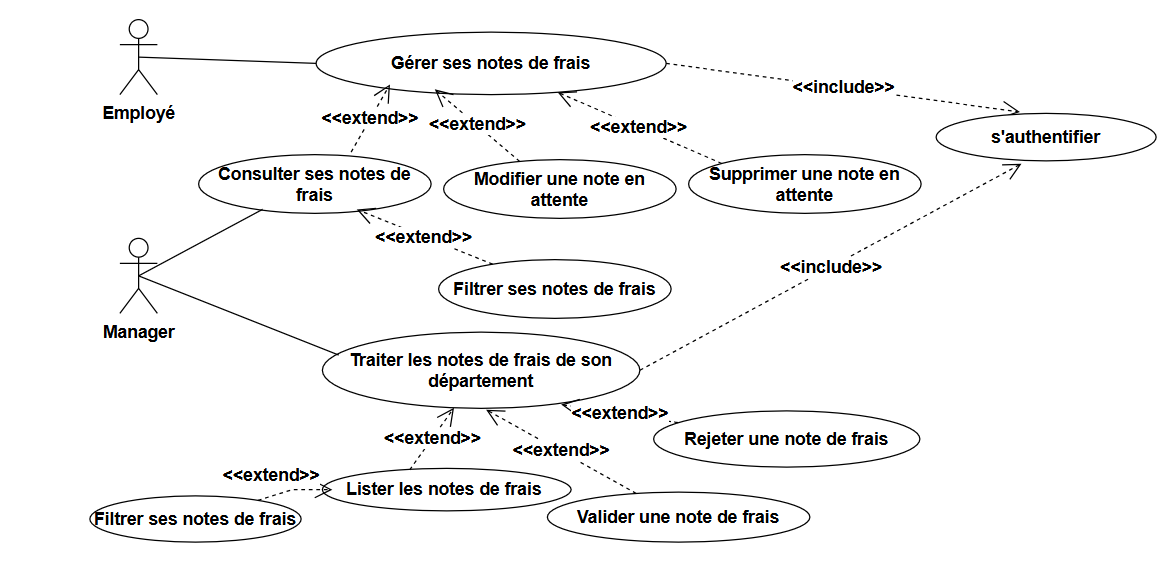
\includegraphics[width=1\textwidth]{usecasesp2.png}

 \caption{Diagramme de cas d'utilisation global du sprint 2}

 \label{fig:usecasesp2}

\end{figure}









\subsection{Descriptions textuelles des cas d’utilisation}

\subsubsection{Description textuelle – Créer et soumettre une note de frais }

\captionof{table}{Description textuelle – Créer et soumettre une note de frais}

\label{tab:create_expense_desc}

\begin{longtable}{|p{3.5cm}|p{11cm}|}

\hline

\textbf{Élément} & \textbf{Description} \\

\hline

\endfirsthead

\hline

\textbf{Élément} & \textbf{Description} \\

\hline

\endhead

\hline

\multicolumn{2}{|c|}{\textit{Suite dans la page suivante}} \\

\hline

\endfoot

\hline

\endlastfoot

Titre & Créer et soumettre une note de frais \\

\hline

Acteur & Employé \\

\hline

But & Remplir une nouvelle note de frais et la soumettre au manager pour validation \\

\hline

Précondition & L'employé est authentifié. \\

\hline

\multirow{12}{*} \newline {\centering Scénario nominal} & 1. L'employé accède à la page « Ajouter une note de frais ». \\

& 2. Le système initialise un formulaire vide. \\

& 3. L'employé sélectionne un projet actif (liste filtrée par son département). \\

& 4. Pour chaque ligne de frais (une ligne est fournie par défaut) :

 \begin{itemize}

 \item[a.] Il choisit une catégorie de dépense (ex: Transport, Hébergement).

 \item[b.] Le système affiche dynamiquement les champs personnalisés de cette catégorie (ex: nombre de nuits, kilométrage, type de repas).

 \item[c.] L'employé saisit la date de la dépense (validation automatique des week-ends et jours fériés tunisiens), le montant (dans la devise courante) et une description.

 \item[d.] Il dépose un justificatif.

 \end{itemize} \\

& 5. L'employé joint l'accord de la société (fichier obligatoire). \\

& 6. Il peut cliquer sur « Enregistrer brouillon » ou « Soumettre la note ». \\

& 7. S'il clique sur « Soumettre » : le système crée la note de frais avec le statut \texttt{EN\_ATTENTE} et enregistre le montant en TND. \\

& 8. Le système envoie une notification in-app et un email au manager du département concerné. \\

& 9. L'employé est redirigé vers la page « Mes notes de frais » et un message de succès s'affiche. \\

\hline

\multirow{5}{*} {Scénario alternatif} & \textbf{Cas de brouillon (stockage local) :} \\

& 5.1. L'employé clique sur « Enregistrer brouillon » → les données sont stockées dans \texttt{localStorage} sans appel au backend. \\

& 5.2. Lors d'une visite ultérieure, le système charge automatiquement le brouillon sauvegardé. \\

& \\

& \textbf{Cas de champ obligatoire manquant ou invalide :} \\

& 6.1. Si un champ requis n'est pas rempli ou est invalide, le système souligne le champ et affiche un message d'erreur spécifique. \\

& 6.2. Le bouton « Soumettre » reste désactivé tant qu'un champs obligatoire n'est pas valide. \\

& \\





\hline

Post-condition & La note est persistée en base (statut \texttt{EN\_ATTENTE}) et les fichiers sont stockés. Le manager reçoit une notification. \\

\hline

\end{longtable}



\newpage

\subsubsection{Description textuelle – Modifier une note de frais}

\captionof{table}{Description textuelle – Modifier une note de frais}

\label{tab:edit_expense_desc}

\begin{longtable}{|p{3.5cm}|p{11cm}|}

\hline

\textbf{Élément} & \textbf{Description} \\

\hline

Titre & Modifier une note de frais \\

\hline

Acteur & Employé \\

\hline

But & Modifier une note de frais en attente \\

\hline

Précondition & L'employé est authentifié et possède une note en statut \texttt{EN\_ATTENTE} \\

\hline

\multirow{6}{*} {Scénario nominal} & 1. L'employé accède à la page « Mes notes de frais ». \\

& 2. Le système affiche la liste paginée de toutes ses notes. \\

& 3. L'employé localise la note à modifier (statut \texttt{EN\_ATTENTE}) et clique sur le bouton « Modifier ». \\

& 4. Le système affiche le formulaire d'ajout pré-rempli avec les informations de la note. \\

& 5. L'employé modifie les champs souhaités (lignes, montants, justificatifs, accord). \\

& 6. Il clique sur le bouton « Modifier ». \\

& 7. Le système valide les données et met à jour la note. \\

& 8. Un message de succès s'affiche et l'employé est redirigé vers la liste des notes. \\

\hline

\multirow{2}{*}{Scénario alternatif} & 2.1 Si la note n'est plus en statut \texttt{EN\_ATTENTE}, le bouton « Modifier » est désactivé. \\

& 5.1 Si les données modifiées sont invalides, le système affiche un message d'erreur et bloque l'enregistrement. \\

\hline

Post-condition & La note est mise à jour avec les nouvelles informations \\

\hline

\end{longtable}



\newpage

\subsubsection{Description textuelle – Valider ou refuser une note (Manager)}

\captionof{table}{Description textuelle – Valider ou refuser une note (Manager)}

\label{tab:validate_reject_desc}

\begin{longtable}{|p{3.5cm}|p{11cm}|}

\hline

\textbf{Élément} & \textbf{Description} \\

\hline

Titre & Valider ou refuser une note de frais \\

\hline

Acteur & Manager \\

\hline

But & Prendre une décision sur une note soumise par un employé de son département \\

\hline

Précondition & Le manager est authentifié. La note est au statut \texttt{EN\_ATTENTE}. \\

\hline

\multirow{10}{*} {Scénario nominal} & 1. Le manager accède à la page « Demandes à valider ». \\

& 2. Le système affiche la liste des notes en attente des employés de son département. \\

& 3. Le manager clique sur « Voir » sur une ligne pour ouvrir la popup de détails. \\

& 4. La popup affiche toutes les lignes, les justificatifs, l’accord et le commentaire éventuel existant. \\

& 5. Le manager examine les informations, puis clique sur « Valider » ou « Refuser ». \\

& 6. S’il clique sur « Valider » : une modal s’ouvre lui permettant d’ajouter un commentaire (optionnel). \\

& 7. S’il clique sur « Refuser » : une modal s’ouvre exigeant un commentaire obligatoire. \\

& 8. Le système enregistre la décision : statut passe à \texttt{VALIDEE} ou \texttt{REFUSEE}, enregistre le commentaire, l’identifiant du manager et la date de décision. \\

& 9. Le système envoie une notification in-app et un email à l’employé. \\

& 10. La modal se ferme et la liste des notes est rafraîchie. \\

\hline

 {Scénario alternatif} & \textbf{Refus sans commentaire} : le système affiche une erreur et bloque la soumission. \\

\hline

Post‑condition & La note change de statut. Une notification est envoyée à l’employé. \\

\hline

\end{longtable}





\newpage

\subsubsection{Description textuelle – Changer la devise d’affichage}



\begin{longtable}{|p{3.5cm}|p{11cm}|}

\caption{Description textuelle – Changer la devise d’affichage}

\label{tab:change_currency_desc} \\

\hline

\textbf{Élément} & \textbf{Description} \\

\hline

\endfirsthead



\hline

\textbf{Élément} & \textbf{Description} \\

\hline

\endhead



\hline

\multicolumn{2}{|c|}{\textit{Suite dans la page suivante}} \\

\hline

\endfoot



\hline

\endlastfoot



Titre & Changer la devise d’affichage \\

\hline

Acteur & Utilisateur (Employé, Manager) \\

\hline

But & Sélectionner une devise (TND, EUR, USD) pour visualiser tous les montants convertis \\

\hline

Précondition & L'utilisateur est authentifié. \\

\hline

\multirow{6}{*} {Scénario nominal} & 1. L'utilisateur clique sur son avatar/nom dans la barre de navigation, puis sur l'option « Devise préférée » dans le menu déroulant. \\

& 2. Le système affiche la liste des devises disponibles (TND, EUR, USD) avec leur symbole et leur nom. \\

& 3. L'utilisateur sélectionne une devise (ex: EUR). \\

& 4. Le système met à jour la devise courante et recharge les taux de change (ou utilise les taux en cache). \\

& 5. Tous les montants affichés dans l'application (tableaux, détails, formulaires) sont immédiatement convertis. \\

& 6. La préférence est sauvegardée dans \texttt{localStorage} et réutilisée lors des connexions ultérieures. \\

\hline

Scénario alternatif & API de taux indisponible : le système utilise les derniers taux en cache et affiche un message d'information. \\

\hline

Post-condition & La devise d'affichage est changée pour toute l'application. \\

\hline

\end{longtable}



\newpage





% =========================

% Diagramme de séquence

% =========================

\section{Conception}

\subsection{Diagrammes de séquence}



\subsubsection{Soumission d'une note avec décision du manager}







\begin{figure}[H]

\centering

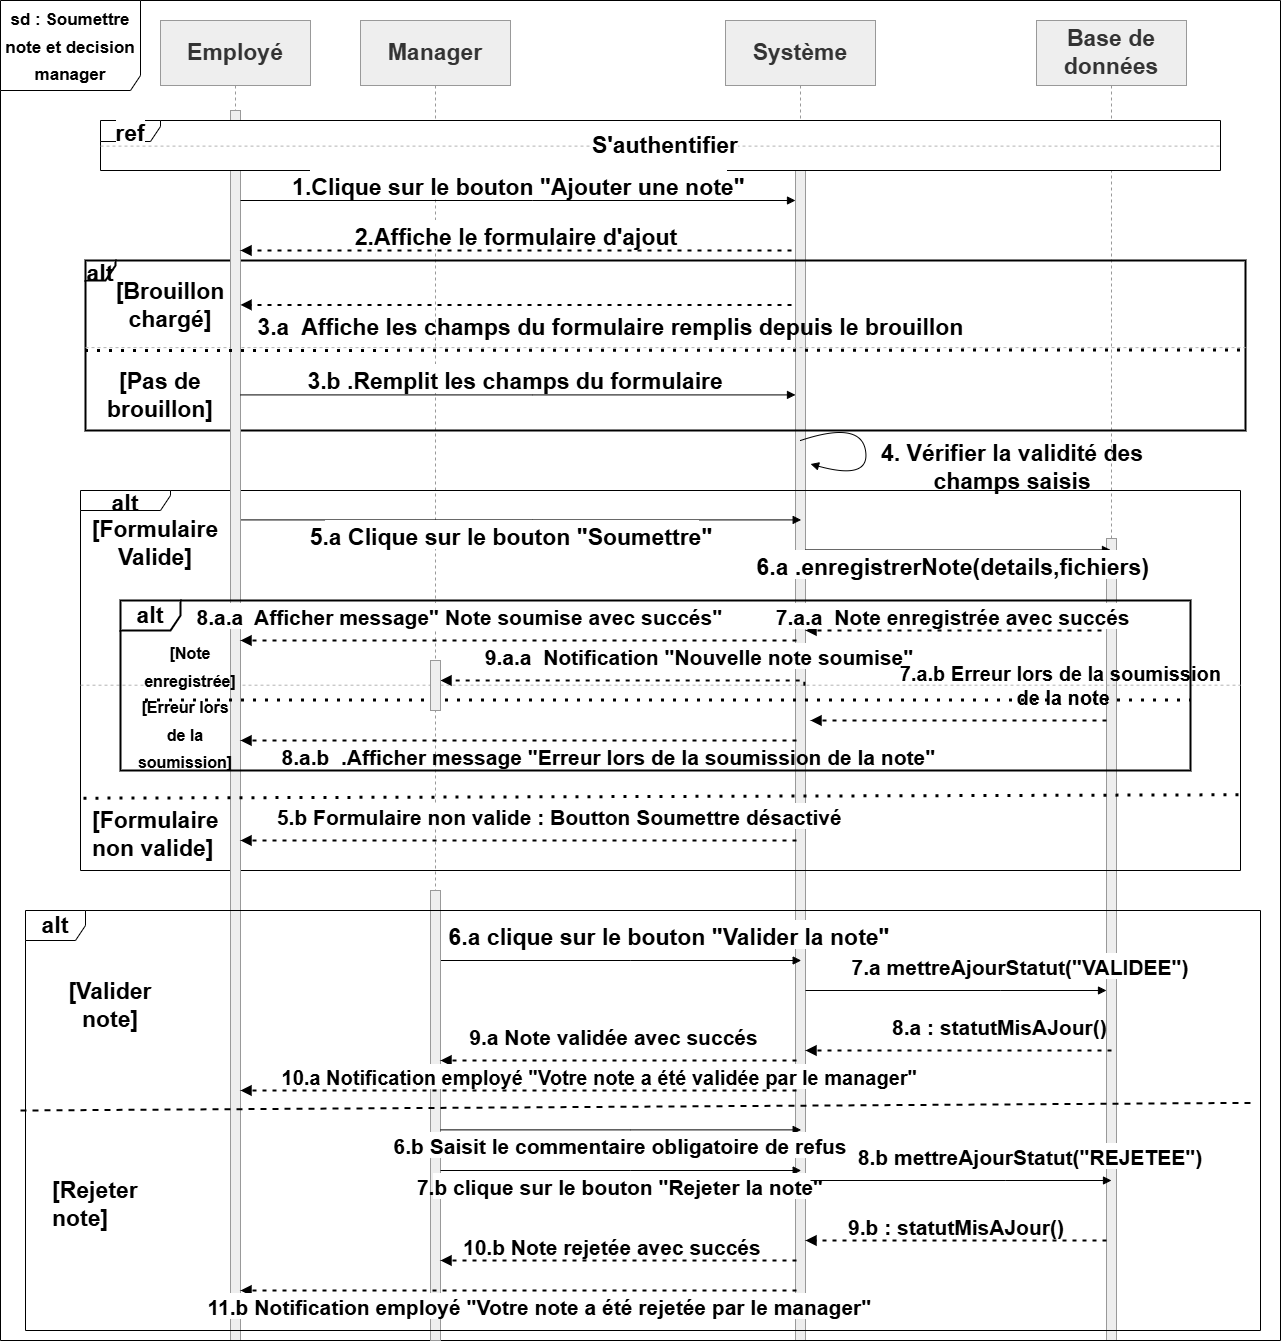
\includegraphics[

 width=\textwidth,

 keepaspectratio,

 height=0.9\textheight % Réduit à 45% de la page

]{sequence_submit_note.png}

\caption{Diagramme de séquence – Soumission d'une note et décision du manager}

\label{fig:seq_submit}

\end{figure}

\noindent

% =========================

% Diagramme de classes

% =========================



\subsection{Diagramme de classes du sprint 2}



\begin{figure}[H]

\centering

\rotatebox{90}{

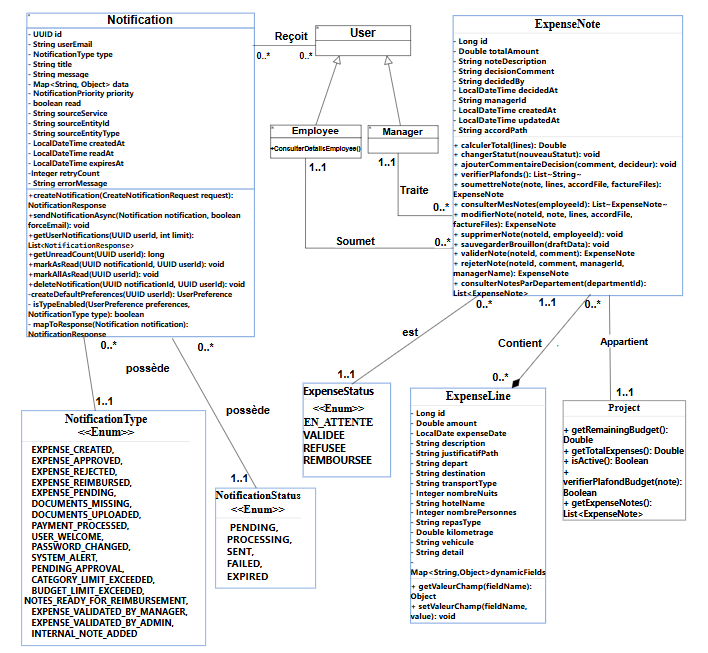
\includegraphics[

 width=0.9\textheight,

 height=1.3\textwidth,

 keepaspectratio

]{diag_classe_sp2.png}

}

\caption{Diagramme de classes du sprint 2}

\label{fig:class_sprint2}

\end{figure}

\section{Interfaces développées}



\subsection{Page « Ajouter une note de frais » }

\subsubsection{Interface d'ajout d'une note de frais}

Cette interface permet à l'employé de créer une nouvelle note de frais. Il sélectionne d'abord un projet actif, puis pour chaque ligne de frais : choisit une catégorie (déclenchant l'affichage des champs personnalisés et du plafond), dépose un justificatif, saisit la date, le montant et une description, puis remplit les champs personnalisés. L'employé joint également l'accord de la société, confirme la lisibilité des documents via des cases à cocher, et peut soit enregistrer un brouillon soit soumettre la note. Une barre de progression suit l'état des justificatifs.

\begin{figure}[H]

\centering

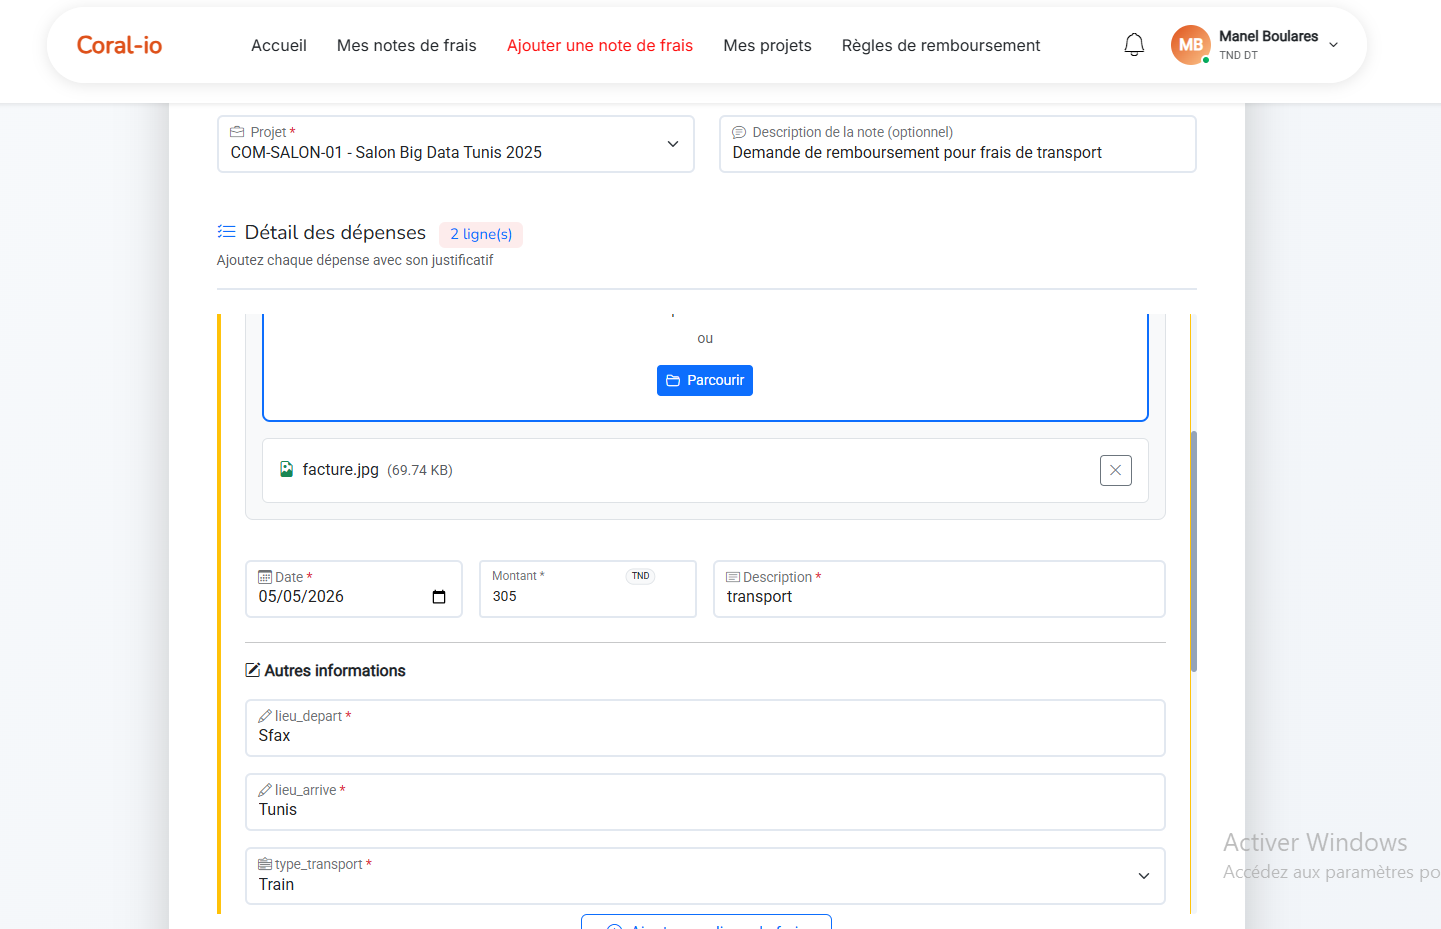
\includegraphics[width=1\textwidth,height=0.5\textheight]{add_note.png}

\caption{Formulaire d’ajout de note de frais}

\label{fig:add_note_ui}

\end{figure}

\begin{figure}[H]

\centering

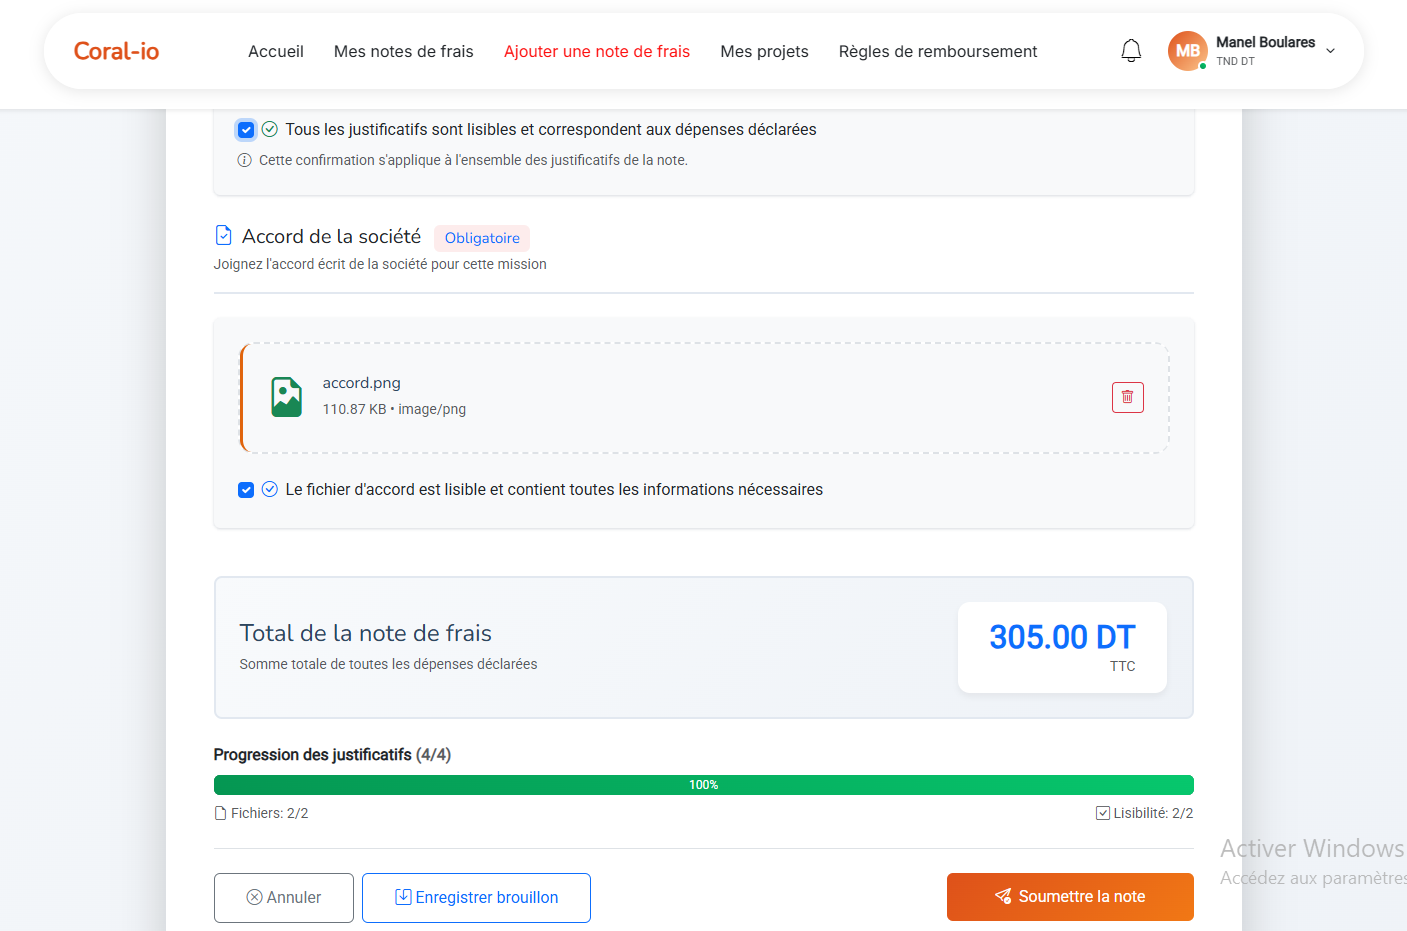
\includegraphics[width=1\textwidth,height=0.5\textheight]{suite_add_note.png}

\caption{Suite du formulaire d’ajout de note de frais}

\label{fig:add_note_ui}

\end{figure}





\subsection{Page « Mes notes de frais »}

\subsubsection{Interface « Mes notes de frais »}

Cette interface permet à l'employé de consulter, filtrer et gérer l'ensemble de ses notes de frais via un tableau paginé avec les colonnes : Projet, Date de création, Total, Statut et Actions. L'utilisateur peut appliquer des filtres par statut, projet, période ou recherche textuelle. Pour chaque note, un bouton « Détails » ouvre une popup de visualisation, et si la note est en statut \texttt{EN\_ATTENTE}, des boutons « Modifier » et « Supprimer » sont disponibles. Un en-tête avec une icône de notification affiche le nombre de non‑lues, et un bouton « Nouvelle note » est placé en haut du tableau.



\begin{figure}[H]

 \centering

 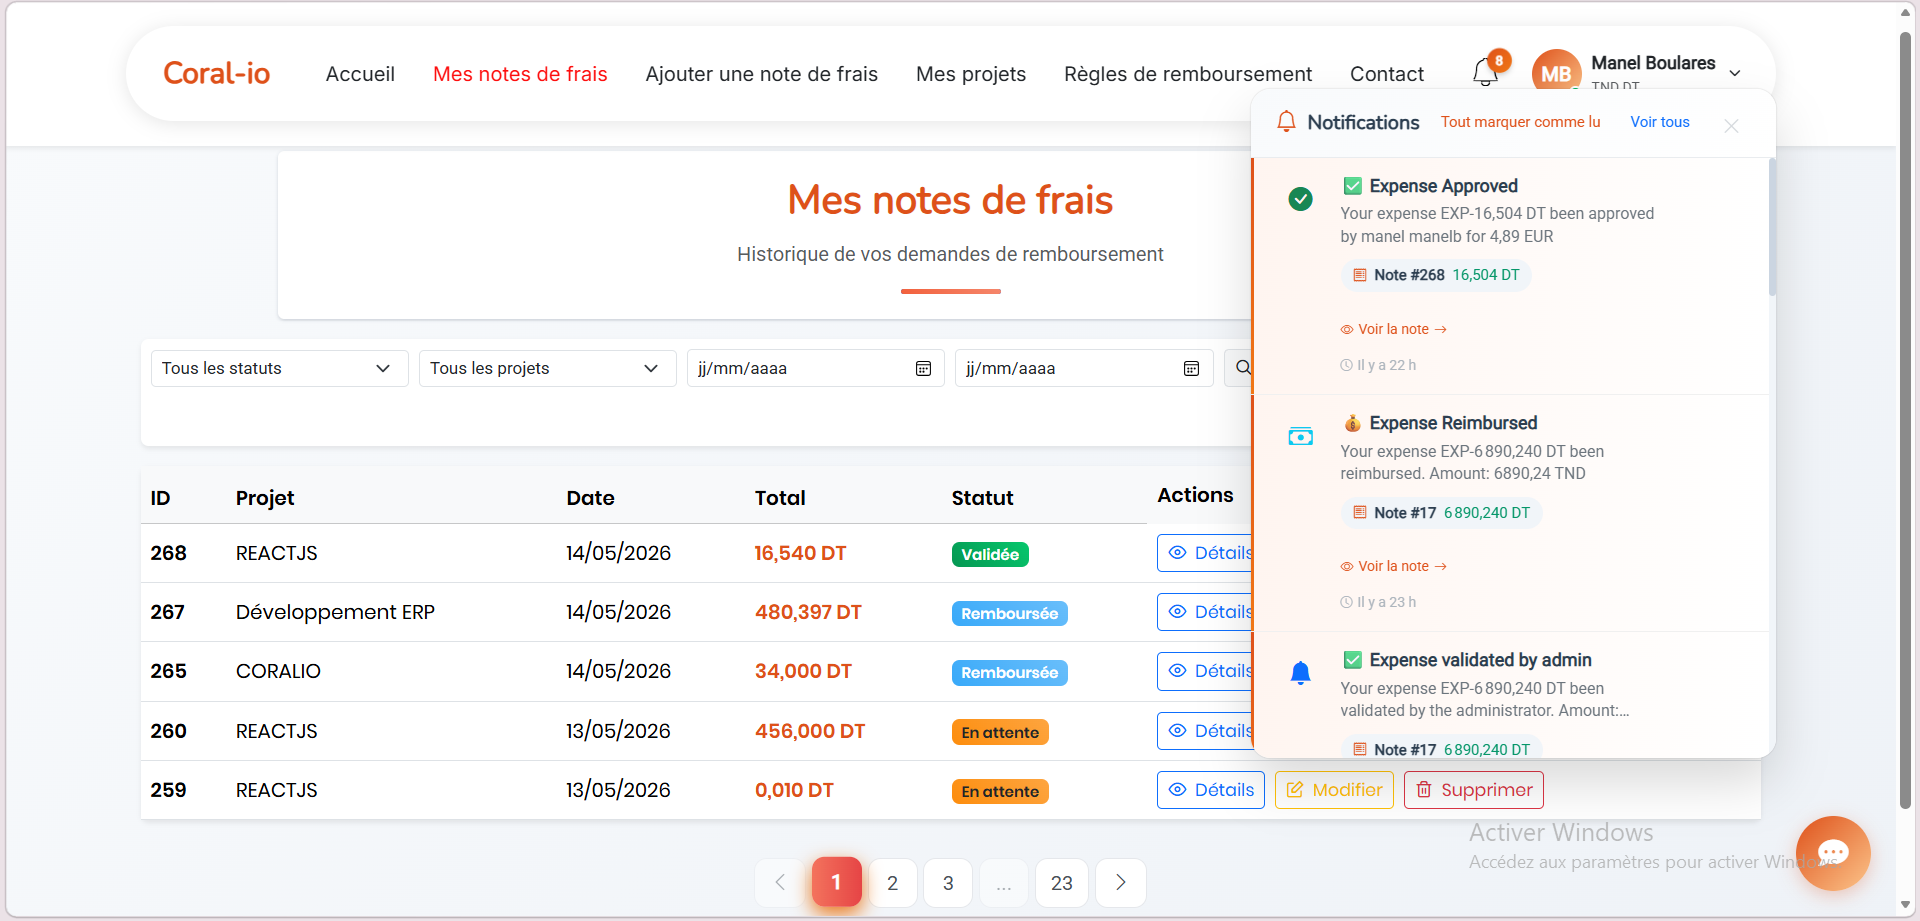
\includegraphics[width=\textwidth]{my_notes.png}

 \caption{Liste des notes de l’employé avec filtres et actions}

 \label{fig:my_notes_ui}

\end{figure}

\subsubsection{Modal de confirmation de suppression d'une note}

Lorsque l'employé clique sur le bouton « Supprimer » pour une note en attente, un modal de confirmation s’affiche afin d’éviter toute suppression accidentelle. Ce modal présente une icône de corbeille animée, un titre « Confirmer la suppression » et un message d’avertissement indiquant que l’action est irréversible. Les détails de la note sont récapitulés. L’utilisateur peut soit annuler, soit confirmer la suppression. Pendant le traitement, un indicateur de chargement désactive le bouton de confirmation. Ce mécanisme garantit une expérience utilisateur sécurisée et prévient les erreurs de manipulation.



\begin{figure}[H]

 \centering

 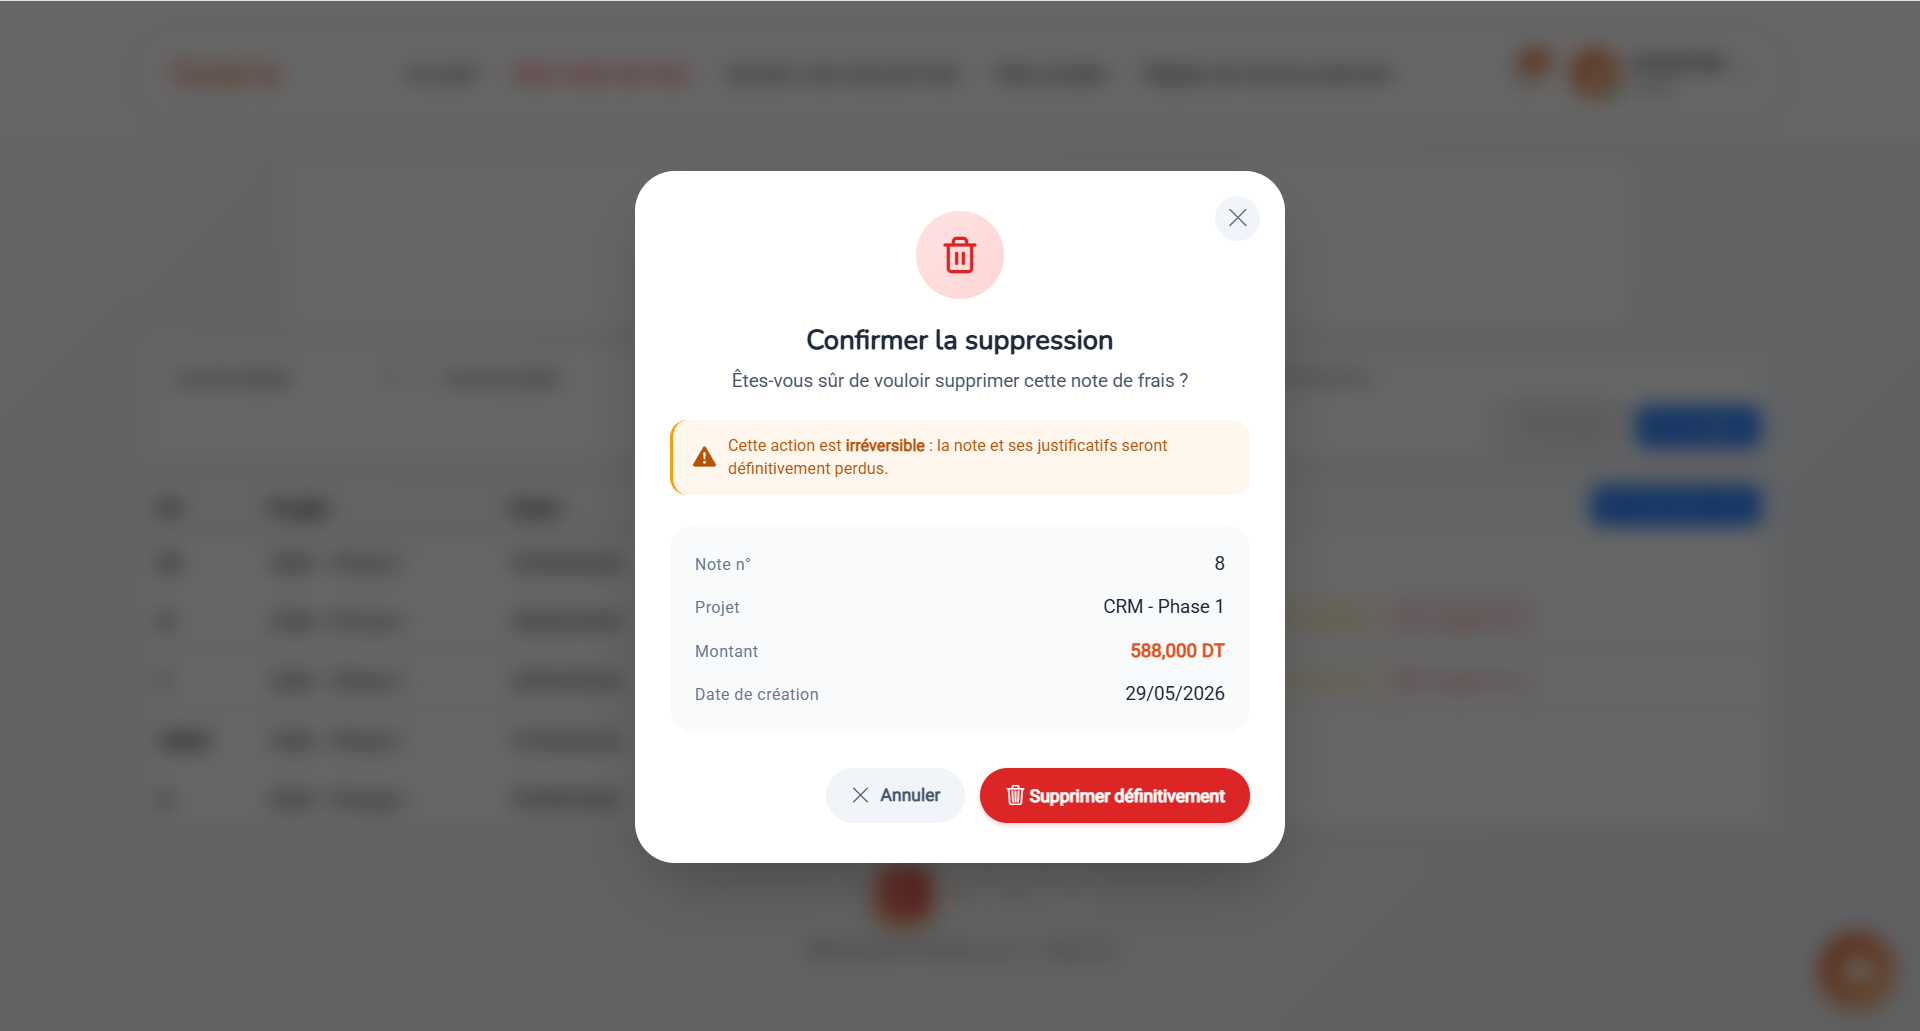
\includegraphics[width=\textwidth]{delete_modal.png}

 \caption{Modal de confirmation de suppression d’une note}

 \label{fig:delete_modal}

\end{figure}





\subsection{Page manager « Demandes à valider » }

\subsubsection{Interface de gestion des notes pour le manager}

Cette interface permet au manager de consulter les notes de frais des employés de son département via un tableau affichant par défaut les notes en attente, avec les colonnes Employé, Projet, Date de soumission, Total converti dans la devise du manager, Statut et Actions. Des filtres permettent de trier par statut, projet, période ou employé via une recherche textuelle. Pour chaque note, un bouton « Voir » ouvre une popup de détails où, si la note est en statut \texttt{EN\_ATTENTE}, le manager peut la valider avec un commentaire optionnel ou la refuser avec un commentaire obligatoire.

\begin{figure}[H]

\centering

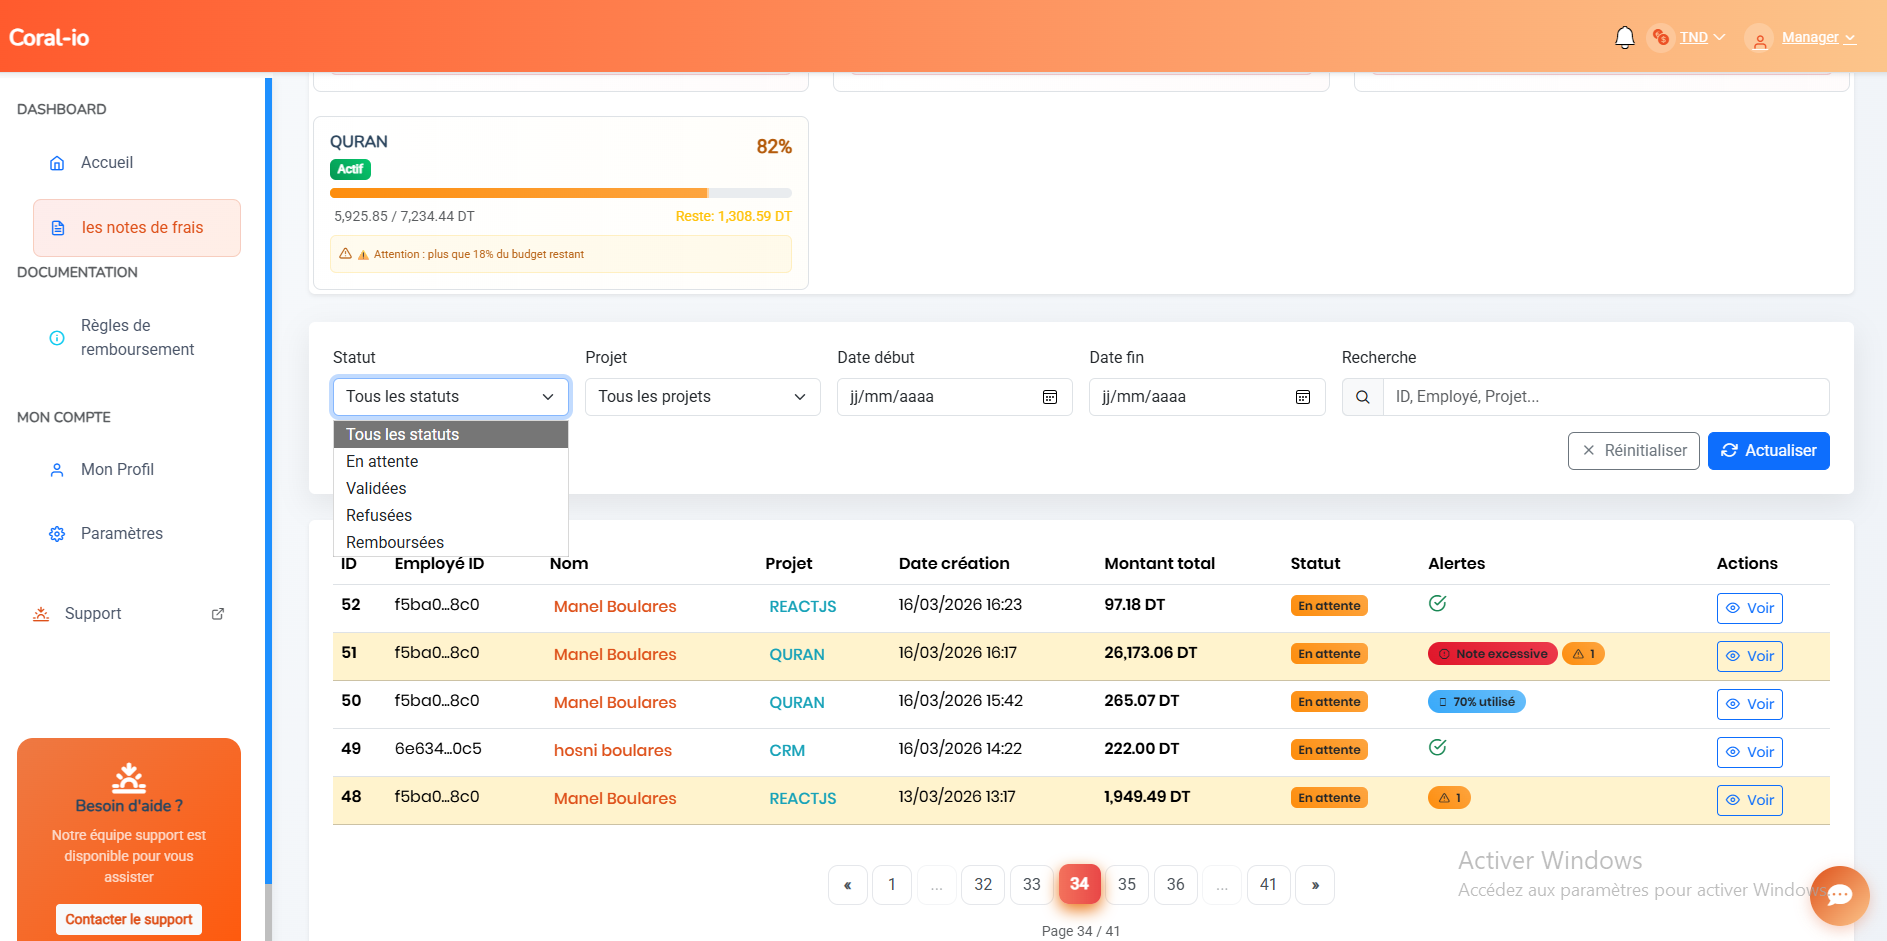
\includegraphics[width=\textwidth]{manager_notes_list.png}

\caption{Liste des notes du département }

\label{fig:manager_notes_ui}

\end{figure}



\subsubsection{Interface de détails d'une note de frais}

Cette interface permet de visualiser l'ensemble des informations d'une note de frais : son en-tête (numéro, date, statut), les informations générales (employé pour le manager et l'admin, projet pour tous), l'accord de la société avec visualisation et téléchargement, le montant total, les alertes de doublons et de dépassement de budget, la description, le commentaire de décision, le tableau des lignes de frais (catégorie, description, date, montant, plafond, justificatif) avec filtres et détails supplémentaires, les notes internes réservées aux managers et administrateurs (consultation, recherche, ajout), ainsi que les boutons d'action adaptés au rôle de l'utilisateur et au statut de la note (Valider/Refuser pour le manager sur une note en attente, Rembourser/Rejeter pour l'admin sur une note validée).

\begin{figure}[H]

\centering

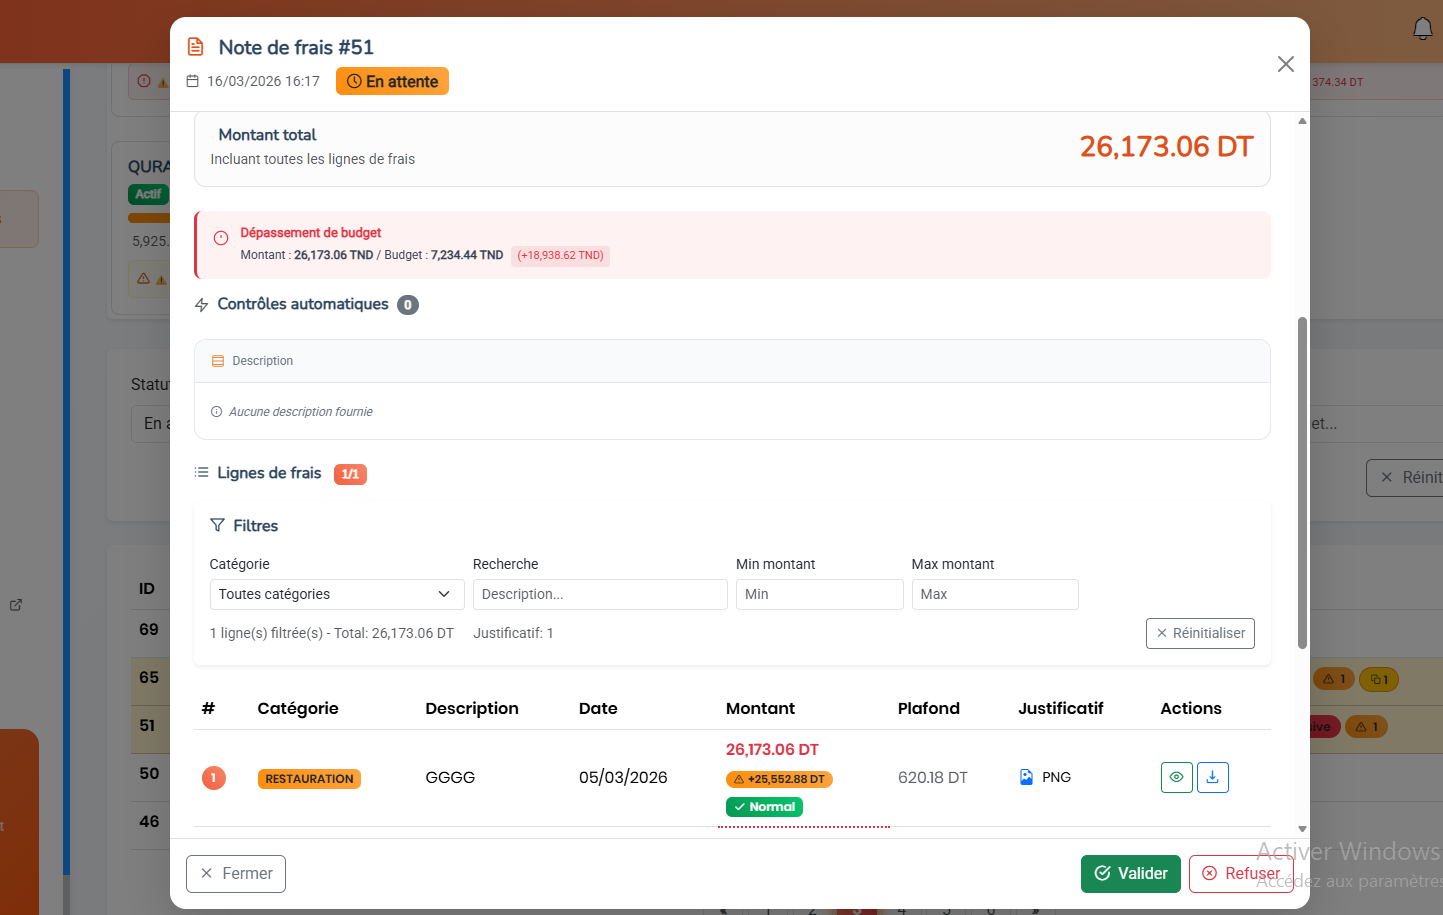
\includegraphics[width=\textwidth]{details_note_sprint2.png}

\caption{Détails d'une note de frais }

\label{fig:details_note}

\end{figure}



\subsection{Interface de consultation de la consommation par employé}

Cette interface, accessible depuis la page des notes de frais du manager ou depuis le tableau de bord administrateur, permet de visualiser pour un employé sélectionné la répartition détaillée de ses dépenses par projet.



\begin{figure}[H]

 \centering

 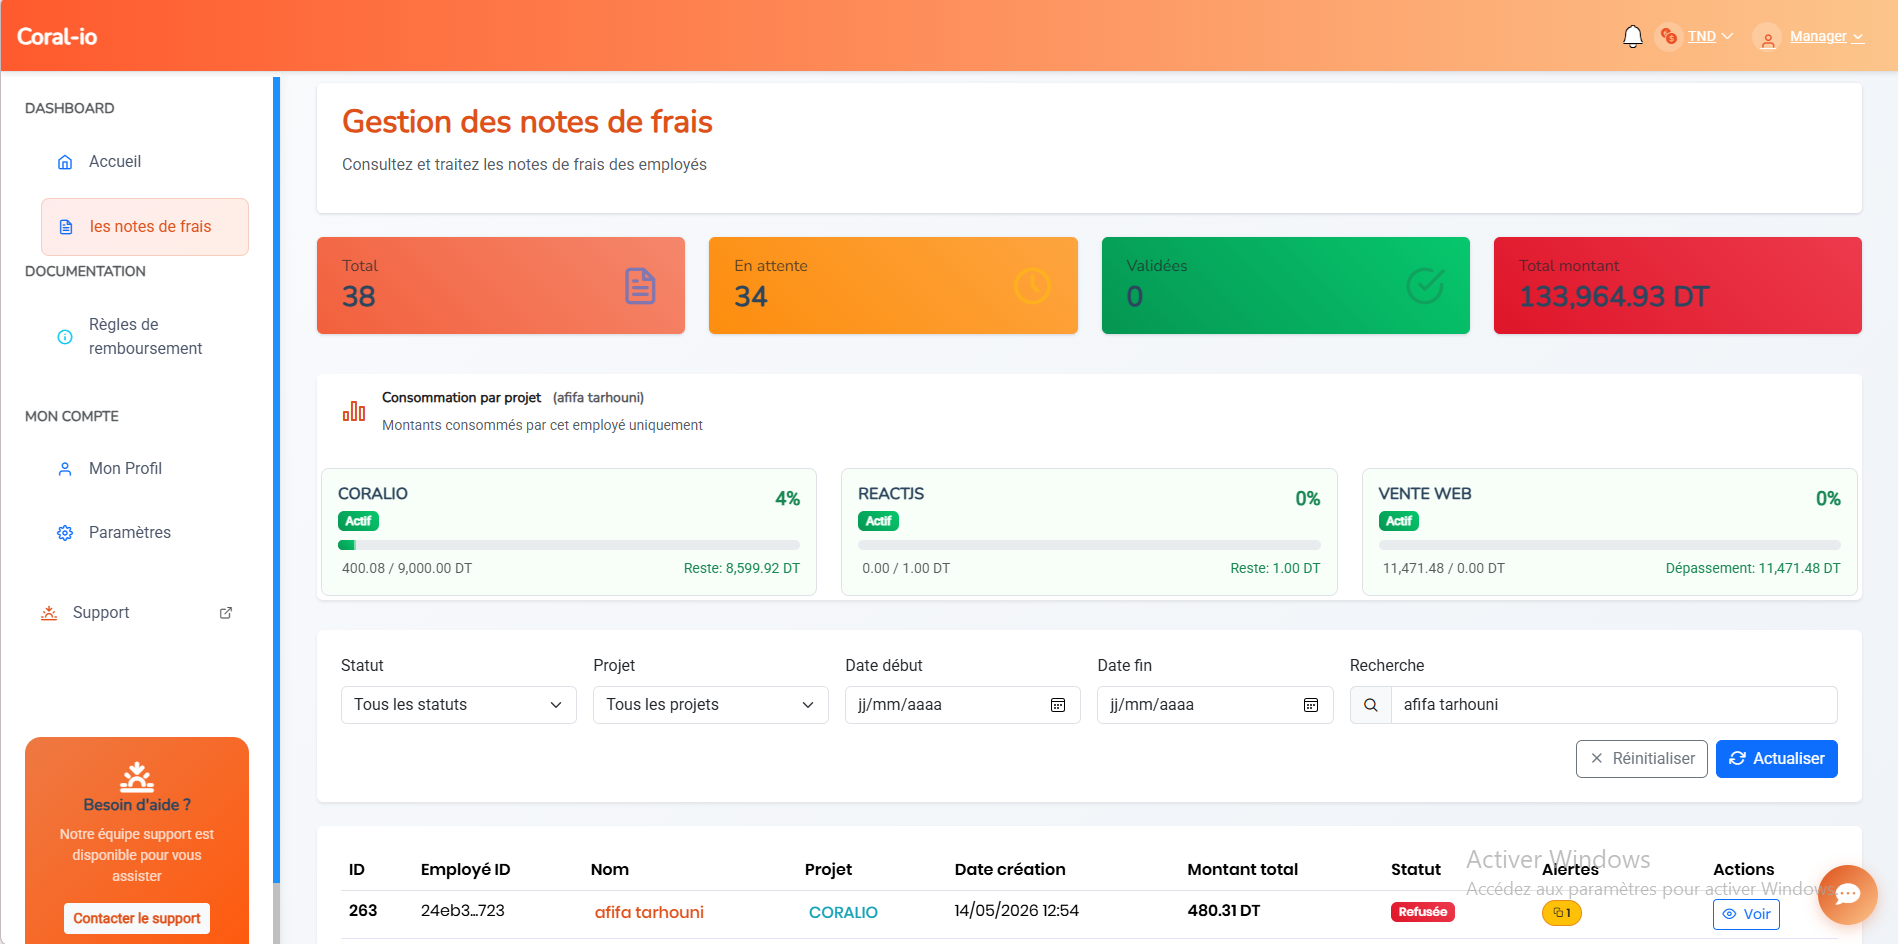
\includegraphics[width=0.9\textwidth]{consommation_employee_sprint2.png}

 \caption{Interface de consultation de la consommation par employé}

 \label{fig:interface_employee_consumption}

\end{figure}

\subsubsection{Modal de validation}

Lorsque le manager clique sur « Valider », une modale s'ouvre avec les éléments suivants : un titre « Valider la note », un message d'alerte en cas de dépassement budgétaire, une section « Utilisation après validation » affichant le budget restant et le nouveau total, les détails de la note (employé et montant), un champ de commentaire optionnel, et les boutons « Valider malgré dépassement » et « Annuler ».

\begin{figure}[H]

\centering

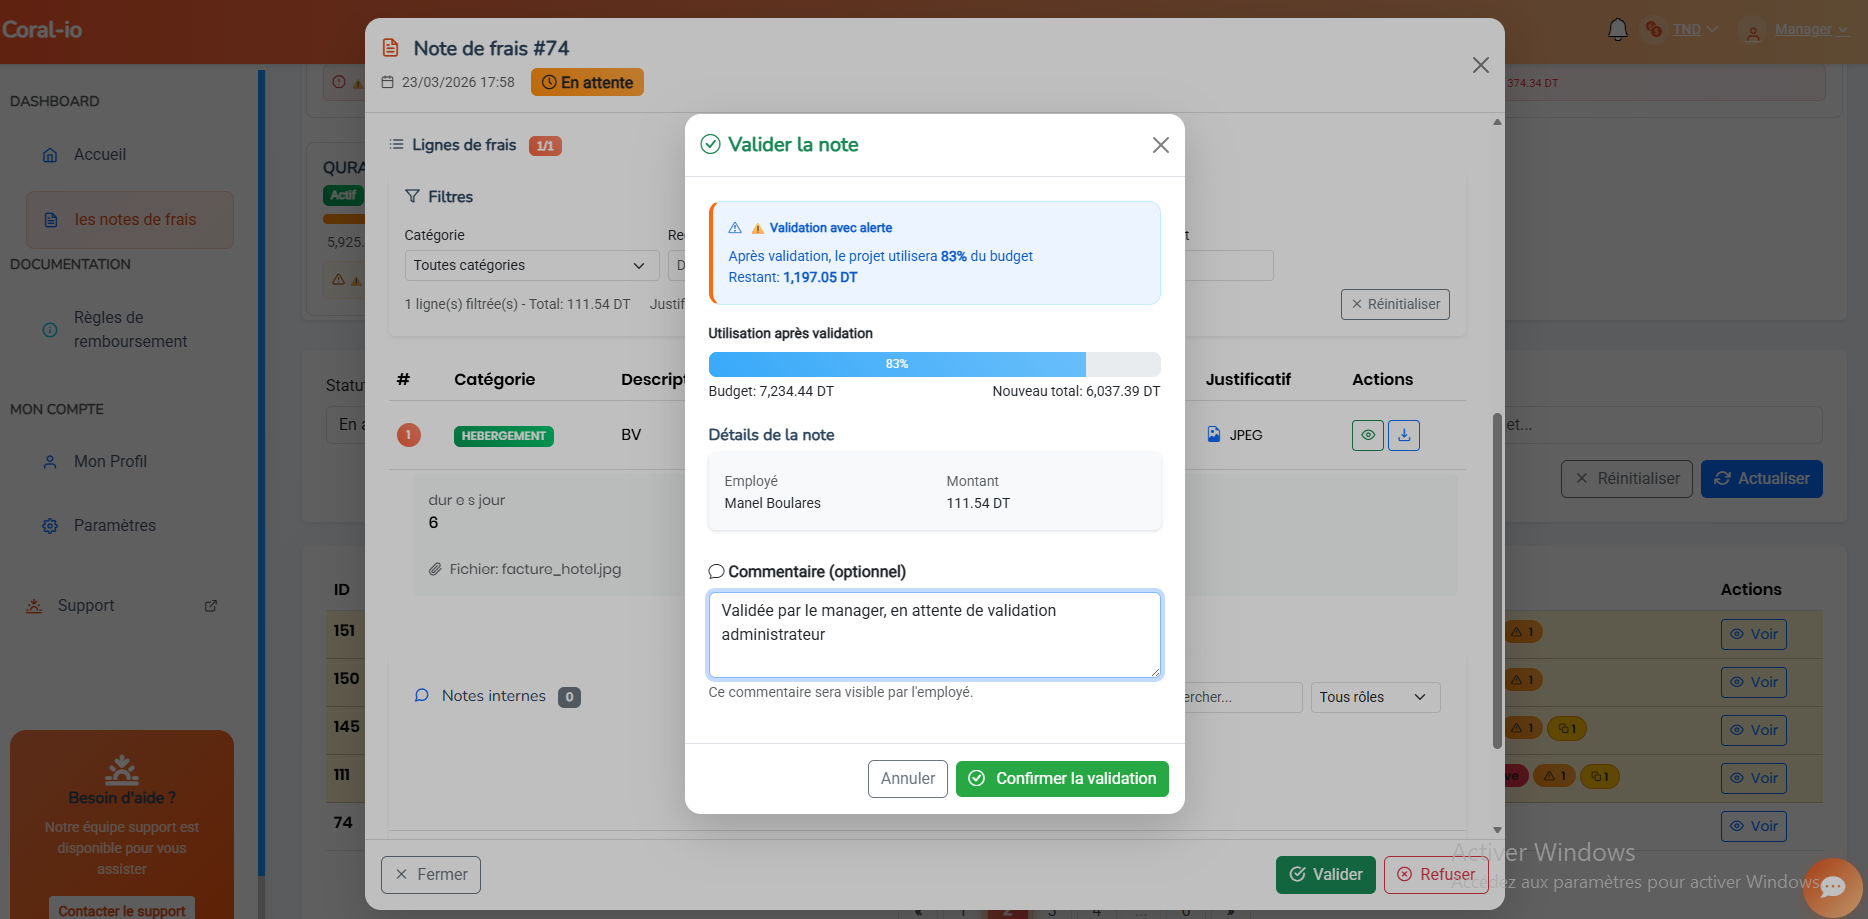
\includegraphics[width=\textwidth]{manager_validate.png}

\caption{Modal de validation }

\label{fig:manager_validation}

\end{figure}

\subsubsection{Modal de refus}

Lorsque le manager clique sur « Refuser », une modale s'ouvre avec les éléments suivants : un titre « Refuser la note », un message d'avertissement « Vous êtes sur le point de refuser la note. Cette action est irréversible », les détails de la note (employé et montant), un champ de commentaire de refus obligatoire, et les boutons « Confirmer le refus » et « Annuler ».



\begin{figure}[H]

\centering

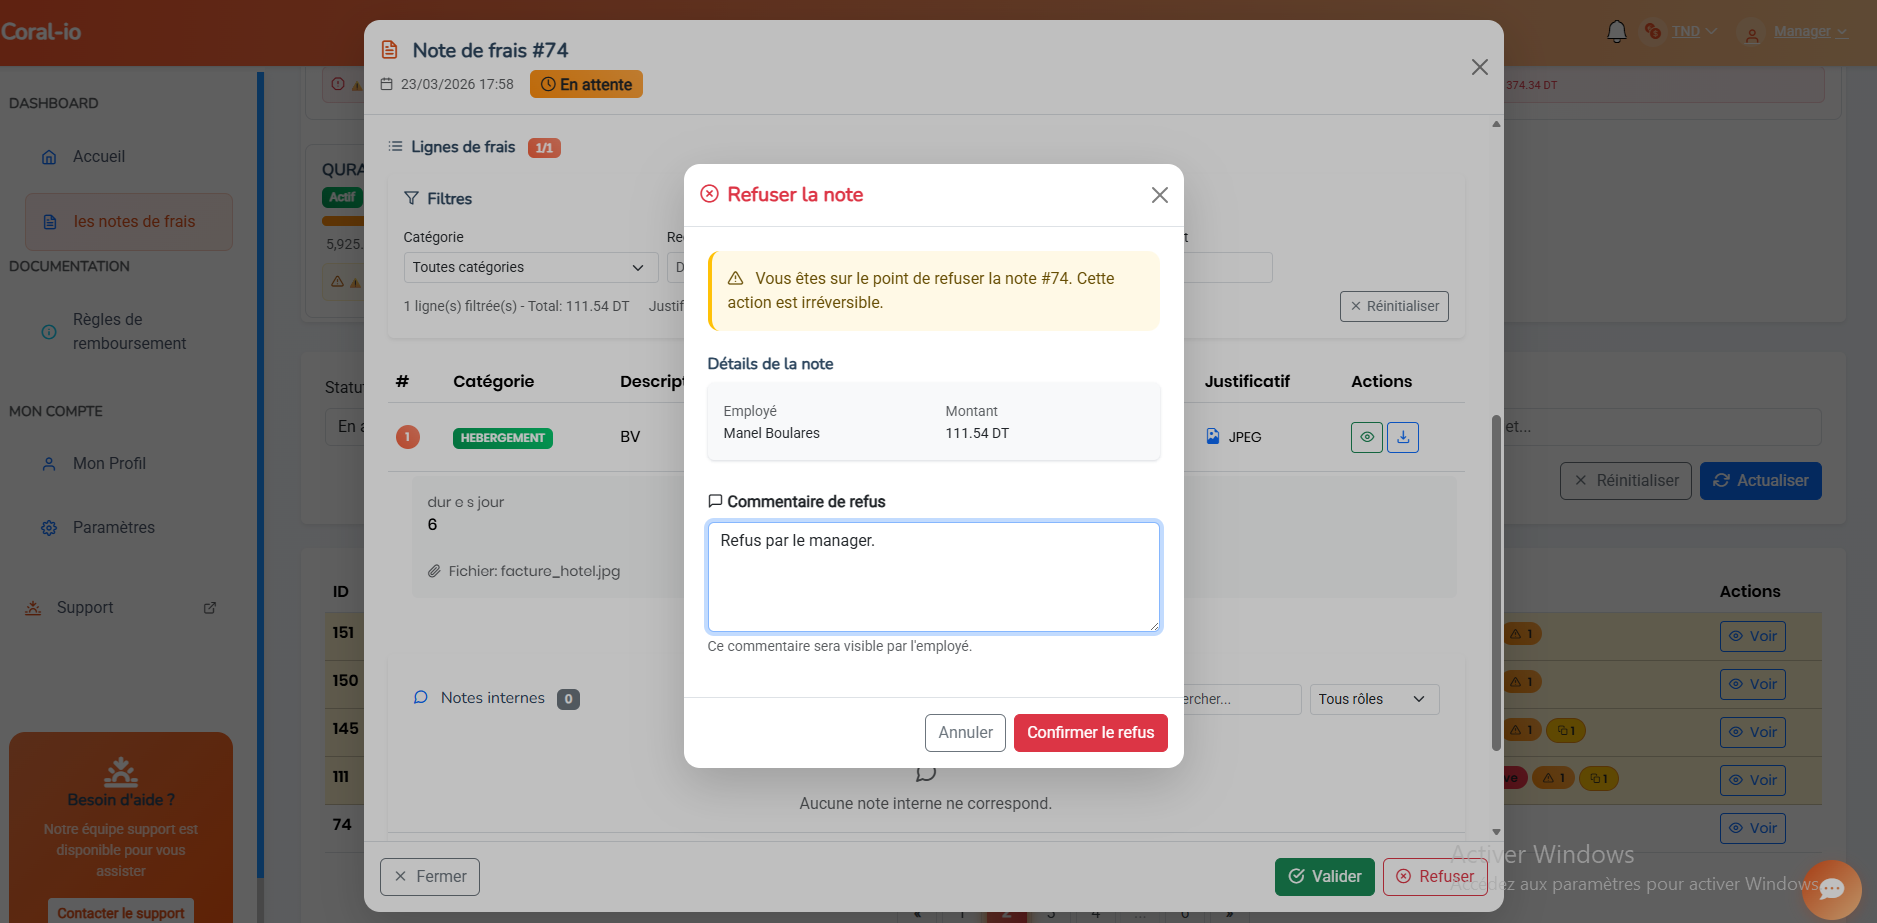
\includegraphics[width=\textwidth]{manager_refus.png}

\caption{Modal de refus }

\label{fig:manager_rejection}

\end{figure}



\subsection{Liste déroulante des notifications}

Ce composant, accessible par une icône de cloche dans l’en‑tête de l’application, regroupe l’ensemble des notifications de l’utilisateur. Les notifications sont classées par ordre chronologique décroissant, avec les non‑lues mises en évidence. Chaque notification affiche le titre, le message, la date et, selon le type, un lien direct vers la note de frais concernée. L’utilisateur peut marquer une notification comme lue en cliquant dessus, supprimer une notification, ou utiliser les boutons « Tout marquer comme lu » et « Effacer tout ». Un badge indique le nombre de notifications non‑lues. Ce système permet à l’utilisateur de rester informé des événements importants sans quitter la page courante.



\begin{figure}[H]

 \centering

 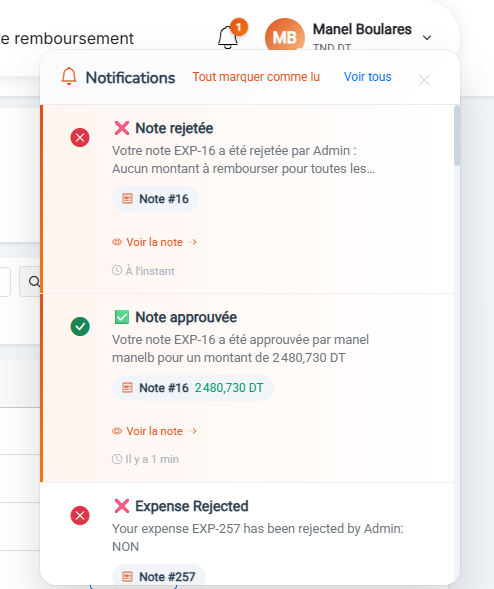
\includegraphics[width=0.5\textwidth]{notificaton_employee.png}

 \caption{Liste déroulante des notifications pour un employé}

 \label{fig:dropdown_notifications}

\end{figure}

\begin{figure}[H]

 \centering

 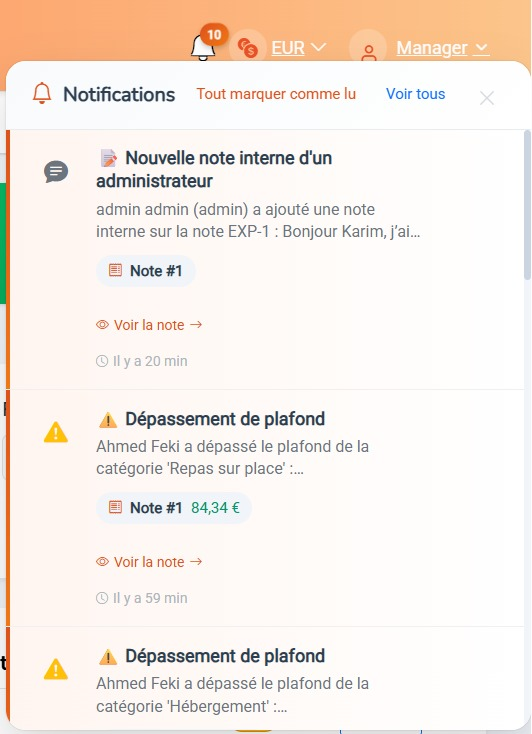
\includegraphics[width=0.4\textwidth]{notification manager.jpeg}

 \caption{Liste déroulante des notifications pour un manager}

 \label{fig:dropdown_notifications}

\end{figure}

\begin{figure}[H]

 \centering

 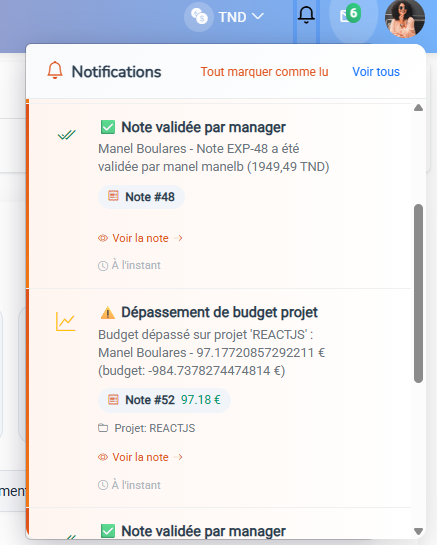
\includegraphics[width=0.4\textwidth]{admin_notification.png}

 \caption{Liste déroulante des notifications pour un administrateur}

 \label{fig:dropdown_notifications}

\end{figure}

\subsubsection{Interface d'historique des notifications}

Cette interface permet à l'utilisateur (employé, manager ou administrateur) de consulter l'ensemble de ses notifications reçues. L'écran affiche la liste paginée des notifications avec la possibilité de charger plus d'éléments via un bouton « Charger plus ». Chaque notification est présentée sous forme de carte affichant son titre, son message, sa date de réception, ainsi que des informations contextuelles telles que le numéro de la note concernée, son montant, le nom du projet et le budget restant en cas d'alerte. Les notifications non lues sont mises en évidence par une bordure colorée et un fond légèrement teinté. L'utilisateur peut marquer une notification comme lue, la supprimer ou cliquer sur « Voir la note » pour être redirigé vers la fiche détaillée de la dépense concernée.

\begin{figure}[H]

\centering

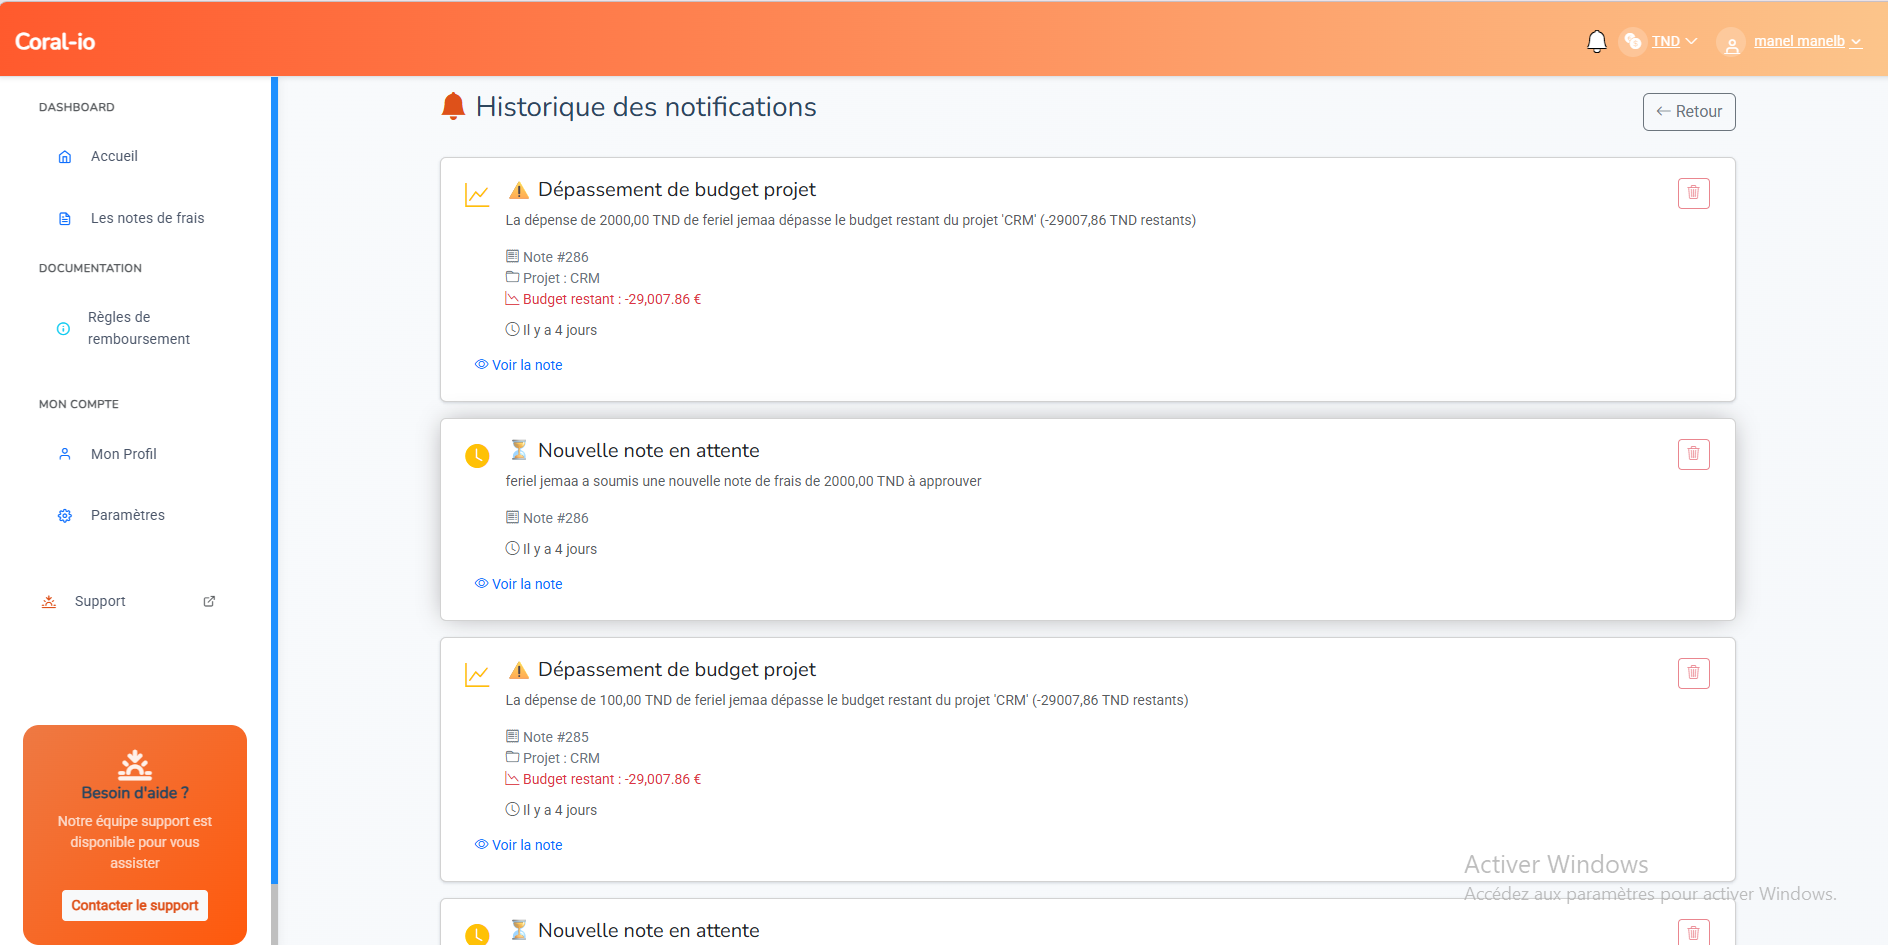
\includegraphics[width=\textwidth]{notification_history.png}

\caption{Interface historique des notifications }

\label{fig:notification_history}

\end{figure}



\section*{Conclusion}

\addcontentsline{toc}{section}{Conclusion}

Le deuxième sprint a livré une gestion complète des notes de frais pour l’employé et le manager, conformément aux US-12 à US-22. Les fonctionnalités implantées sont : création/soumission, consultation avec filtres, modification/suppression (notes en attente), validation/refus par manager avec commentaire, notifications, multi‑devises. L’architecture technique repose sur les services déjà mis en place au sprint 1. Le sprint suivant (sprint 3) traitera les remboursements, les ordres de paiement et les notifications associées.



\chapter{Sprint 3 « Remboursement et déploiement»}



\section*{Introduction}

\addcontentsline{toc}{section}{Introduction}

Ce chapitre présente le Sprint 3 dédié au « Workflow de validation, remboursement et déploiement ». Nous détaillerons le Backlog du sprint, les diagrammes de séquence, les étapes de conception et les interfaces développées.



\section{Objectif du sprint}

L'objectif de ce sprint est de finaliser le cycle de vie d'une note de frais et de préparer l'environnement de production, en permettant à l'administrateur de traiter les notes validées par le manager de déployer l'ensemble des microservices via Docker et Docker Compose.



\section{Backlog du sprint 3}



\subsection{Décomposition du sprint 3}



Le tableau ci-dessous illustre la décomposition du sprint 3. La durée totale du sprint 3 est de 20 jours ouvrables (du 31/03 au 27/04).

\captionof{table}{Backlog Sprint 3}

\label{tab:sprint3_combined}

\begin{longtable}{|c|p{5cm}|p{5.5cm}|c|}

\hline

\textbf{ID} & \textbf{User Story} & \textbf{Tâches techniques} & \textbf{Durée (jours)} \\

\hline

\endfirsthead



\hline

\textbf{ID} & \textbf{User Story} & \textbf{Tâches techniques} & \textbf{Durée (jours)} \\

\hline

\endhead



\hline

\multicolumn{4}{|c|}{\textit{Suite dans la page suivante}} \\

\hline

\endfoot



\hline

\endlastfoot



US-49 & En tant qu'employé et manager, je veux être alerté (in-app et email) de tout événement critique sur les notes de frais (validation, refus, remboursement, rejet, soumission, ajout de note interne) afin de suivre l’évolution des demandes et de réagir rapidement. & 

\begin{tabular}[t]{@{}p{5.5cm}@{}}

- Extension du microservice de notifications \\

- Frontend: réception et affichage des notifications \\

- Tests

\end{tabular} & 2j \\

\hline

US-50 & En tant qu'administrateur et manager, je veux ajouter une note interne confidentielle à une note de frais, visible uniquement par l'autre partie, afin de communiquer des informations sensibles sans les exposer à l'employé. & 

\begin{tabular}[t]{@{}p{5.5cm}@{}}

- Backend: endpoint ajout note interne \\

- Frontend: champ de saisie note interne dans la popup de détails \\

- Tests

\end{tabular} & 1.5j \\

\hline

US-51 & En tant qu'administrateur, je veux consulter toutes les notes validées par le manager afin de procéder à leur remboursement. & 

\begin{tabular}[t]{@{}p{5.5cm}@{}}

- Backend: endpoints pour lister les notes validées \\

- Frontend: page ValidatedNotesListComponent (liste des notes validées) \\

- Tests

\end{tabular} & 1j \\

\hline

US-52 & En tant qu'administrateur, je veux rembourser une note (total ou partiel) afin d'indemniser l'employé pour les frais légitimes. & 

\begin{tabular}[t]{@{}p{5.5cm}@{}}

- Backend: endpoints remboursement total/partiel \\

- Frontend: page ReimbursementFormComponent (formulaire de remboursement) \\

- Tests

\end{tabular} & 2j \\

\hline

US-53 & En tant qu'administrateur, je veux rejeter le remboursement d'une note avec un commentaire afin d'informer l'employé et le manager de la raison du refus. & 

\begin{tabular}[t]{@{}p{5.5cm}@{}}

- Backend: endpoint rejet de remboursement avec commentaire \\

- Frontend: modal de rejet \\

- Intégration des notifications (remboursement/rejet)

\end{tabular} & 1j \\

\hline

US-54 & En tant qu'administrateur, je veux consulter l'ordre de paiement généré automatiquement par le système après validation d'une note de frais, afin de disposer d'un justificatif traçable et de consulter l'ordre généré. & 

\begin{tabular}[t]{@{}p{5.5cm}@{}}

- Backend: service de génération d’ordre de paiement (PDF) \\

- Conception des diagrammes de séquence et de classe \\

- Tests

\end{tabular} & 1.5j \\

\hline

US-55 & En tant qu'administrateur, je veux consulter les ordres de paiement en attente afin de suivre les paiements à effectuer. & 

\begin{tabular}[t]{@{}p{5.5cm}@{}}

- Backend: endpoints pour ordres de paiement (CRUD, statut EN\_ATTENTE/PAYE/ANNULE) \\

- Frontend: page ReimbursementListComponent (ordres en attente) \\

- Tests

\end{tabular} & 1j \\

\hline

US-56 & En tant qu'administrateur, je veux confirmer le paiement et archiver la note afin de clôturer définitivement le remboursement. & 

\begin{tabular}[t]{@{}p{5.5cm}@{}}

- Backend: service de confirmation de paiement et archivage \\

- Frontend: page OrderDetailsComponent (confirmation paiement) \\

- Tests

\end{tabular} & 1.5j \\

\hline

US-57 & En tant qu'administrateur, je veux consulter l'archive des notes traitées afin de pouvoir retrouver un justificatif en cas d'audit. & 

\begin{tabular}[t]{@{}p{5.5cm}@{}}

- Frontend: page NoteArchiveComponent (archive consolidée) \\

- Backend: endpoints pour récupérer les notes archivées \\

- Tests

\end{tabular} & 1j \\

\hline

US-58 & En tant qu'administrateur, je veux visualiser, avant de confirmer un remboursement, le budget restant du projet et une alerte si le montant à rembourser dépasse ce budget, afin d'éviter de dépasser les enveloppes budgétaires. & 

\begin{tabular}[t]{@{}p{5.5cm}@{}}

- Backend: récupération du budget du projet et calcul du reste \\

- Frontend: affichage d’une alerte dans le modal de remboursement \\

- Tests

\end{tabular} & 1j \\

\hline

US-59 & En tant qu'administrateur, je veux consulter un tableau de bord dédié au suivi des budgets et consommations des projets, afin d'avoir une vision globale de l'état financier des projets. & 

\begin{tabular}[t]{@{}p{5.5cm}@{}}

- Composant Angular \texttt{AdminProjectDashboard} \\

- Intégration des données (budgets, consommations) \\

- Tests

\end{tabular} & 2j \\

\hline

US-60 & En tant qu'administrateur, je veux filtrer les données du tableau de bord projets afin d'analyser la répartition des coûts et de détecter rapidement les dépassements. & 

\begin{tabular}[t]{@{}p{5.5cm}@{}}

- Intégration des filtres (période, statut, seuil critique) \\

- Tests

\end{tabular} & 1j \\

\hline

US-61 & En tant qu'administrateur, je veux exporter les données du tableau de bord projets afin de réaliser des reporting hors ligne ou des analyses externes. & 

\begin{tabular}[t]{@{}p{5.5cm}@{}}

- Export CSV/EXCEL/PDF \\

- Tests

\end{tabular} & 0.5j \\

\hline

US-62 & En tant qu'administrateur, je veux exporter les notes vers Excel afin d'effectuer des analyses externes ou des reporting hors ligne. & 

\begin{tabular}[t]{@{}p{5.5cm}@{}}

- Frontend : service d’export \\

- Frontend : boutons d’export sur les tableaux \\

- Tests

\end{tabular} & 1j \\

\hline

US-63 & En tant que DevOps, je veux dockeriser l'application afin de faciliter le déploiement et l'environnement de test. & 

\begin{tabular}[t]{@{}p{5.5cm}@{}}

- Création des Dockerfiles pour chaque microservice \\

- Configuration de Docker Compose \\

- Tests d’intégration avec conteneurs \\

- Documentation du déploiement

\end{tabular} & 2j \\

\hline

\multicolumn{3}{|c|}{\textbf{Total}} & \textbf{20j} \\

\hline

\end{longtable}







\section{Analyse}



\subsection{Diagramme de cas d'utilisation global du sprint 3}



\begin{figure}[H]

 \centering

 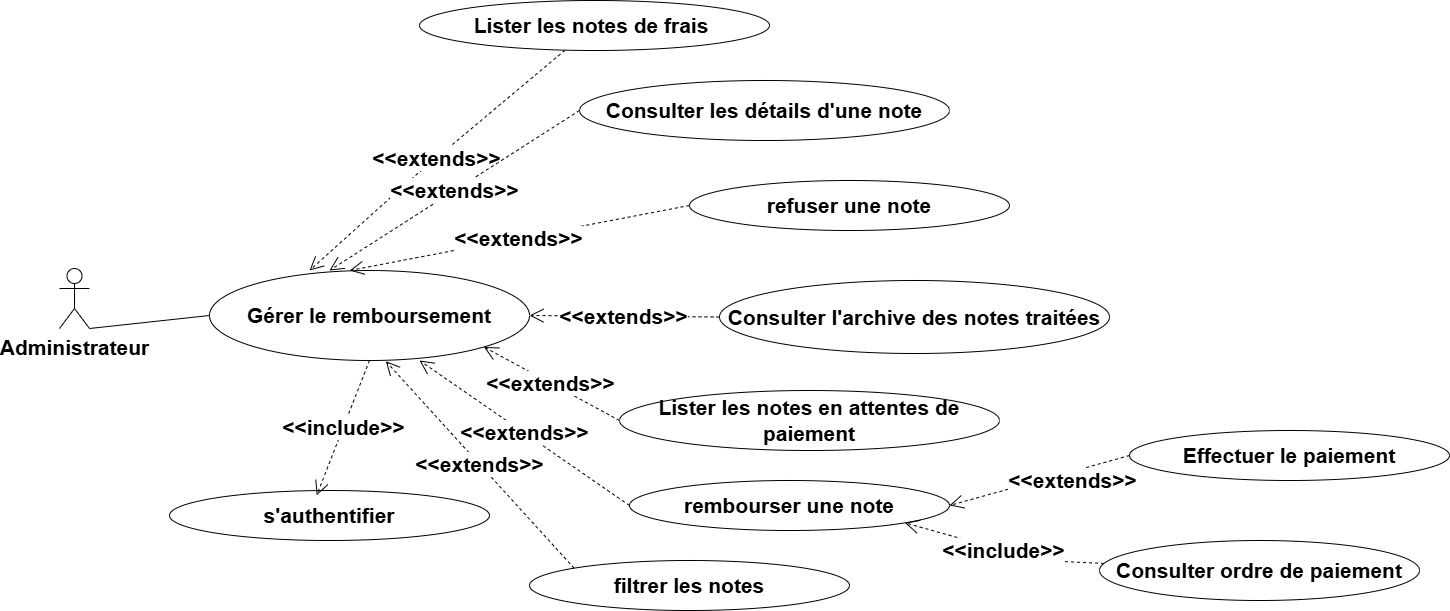
\includegraphics[width=1\textwidth,height=0.4\textheight]{usecasesp3.png}

 \caption{Diagramme de cas d'utilisation global du sprint 3}

 \label{fig:usecasesp3}

\end{figure}







\subsection{Descriptions textuelles des cas d'utilisation}



\subsubsection{Description textuelle – Consulter les notes validées}

\captionof{table}{Description textuelle – Consulter les notes validées}

\label{tab:view_validated_notes_desc}

\begin{longtable}{|p{3.5cm}|p{11cm}|}

\hline

\textbf{Élément} & \textbf{Description} \\

\hline

\endfirsthead

\hline

\textbf{Élément} & \textbf{Description} \\

\hline

\endhead

\hline

\multicolumn{2}{|c|}{\textit{Suite de la page suivante}} \\

\hline

\endfoot

\hline

\endlastfoot

Titre & Consulter les notes de frais validées par le manager \\

\hline

Acteur & Administrateur \\

\hline

But & Visualiser l'ensemble des notes ayant le statut \texttt{VALIDEE} par le manager.\\

\hline

Précondition & L'administrateur est authentifié. \\

\hline

\multirow{5}{*}{Scénario nominal} & 1. L'administrateur accède à la page « Notes à traiter ». \\

& 2. Le système charge la liste des notes dont le statut est \texttt{VALIDEE} et qui ne sont pas déjà associées à un ordre de paiement en attente. \\

& 3. Le système affiche un tableau paginé contenant : le numéro de la note, le nom de l'employé, le projet, le montant total, la date de validation et le statut. \\

& 4. L'administrateur peut filtrer la liste par recherche textuelle, par projet et par intervalle de dates. \\

& 5. Un clic sur une note ouvre une popup de détails permettant de procéder au remboursement ou au refus. \\

\hline

Scénario alternatif & Aucune note validée : le système affiche un message « Aucune note validée trouvée ». \\

\hline

Post-condition & L'administrateur dispose de la liste des notes éligibles au remboursement. \\

\hline

\end{longtable}





\subsubsection{Description textuelle – Rejeter le remboursement d'une note}

\captionof{table}{Description textuelle – Rejeter le remboursement d'une note}

\label{tab:reject_reimbursement_desc}

\begin{longtable}{|p{3.5cm}|p{11cm}|}

\hline

\textbf{Élément} & \textbf{Description} \\

\hline

\endfirsthead



\hline

\textbf{Élément} & \textbf{Description} \\

\hline

\endhead



\hline

\multicolumn{2}{|c|}{\textit{Suite dans la page suivante}} \\

\hline

\endfoot



\hline

\endlastfoot



Titre & Rejeter définitivement le remboursement d'une note \\

\hline

Acteur & Administrateur \\

\hline

But & Refuser la note, avec commentaire obligatoire, et notifier l'employé et le manager \\

\hline

Précondition & L'administrateur est authentifié et la note a le statut \texttt{VALIDEE}. \\

\hline

\multirow{9}{*} {Scénario nominal} & 1. L'administrateur clique sur le bouton « Notes à traiter » dans le menu. \\

& 2. Le système affiche la liste des notes ayant le statut \texttt{VALIDEE}. \\

& 3. L'administrateur clique sur une note pour consulter ces détails. \\

& 4. L'administrateur clique sur le bouton « Refuser » dans la popup de détails. \\

& 5. Une fenêtre modale de confirmation s'ouvre, affichant le numéro de la note, l'employé concerné et le montant total. \\

& 6. L'administrateur saisit obligatoirement un commentaire expliquant le motif du refus. \\

& 7. Il confirme le refus. \\

& 8. Le système change le statut de la note en \texttt{REFUSEE} et enregistre le commentaire. \\

& 9. Le système envoie une notification à l'employé mentionnant le motif du refus. \\

& 10. La modale se ferme et l'administrateur est redirigé vers la page d'archive. \\

\hline

Scénario alternatif & Le commentaire est vide : le système affiche un message d'erreur et bloque la validation. \\

\hline

Post-condition & La note est définitivement refusée et apparaît dans l'archive avec la mention « Refusée ». L'employé est informé. \\

\hline

\end{longtable}





\subsubsection{Description textuelle – Confirmer le paiement d'un ordre}

\captionof{table}{Description textuelle – Confirmer le paiement d'un ordre}

\label{tab:confirm_payment_desc}

\begin{longtable}{|p{3.5cm}|p{11cm}|}

\hline

\textbf{Élément} & \textbf{Description} \\

\hline

\endfirsthead



\hline

\textbf{Élément} & \textbf{Description} \\

\hline

\endhead



\hline

\multicolumn{2}{|c|}{\textit{Suite dans la page suivante}} \\

\hline

\endfoot



\hline

\endlastfoot



Titre & Confirmer le paiement d'un ordre \\

\hline

Acteur & Administrateur \\

\hline

But & Marquer un ordre comme payé, enregistrer la méthode et une référence, et archiver la note \\

\hline

Précondition & L'administrateur est authentifié et la note a le statut \texttt{VALIDEE}. \\

\hline

\multirow{10}{*}{Scénario nominal} & 1. L'administrateur clique sur le bouton « Rembourser » dans la popup de détails de la note ou dans la liste des notes validées. \\

& 2. Le système redirige l'administrateur vers l'interface de détail de l'ordre de paiement. \\

& 3. L'administrateur visualise les informations de l'ordre : numéro, note associée, employé, montant total, liste des lignes remboursées avec montants originaux et remboursés. \\

& 4. Il clique sur le bouton « Confirmer le paiement ». \\

& 5. Une modale s'ouvre, affichant le montant à payer et proposant de choisir la méthode de paiement (virement bancaire, chèque, espèces) et d'ajouter une référence optionnelle (numéro de virement, numéro de chèque). \\

& 6. L'administrateur sélectionne la méthode, saisit éventuellement une référence, puis valide. \\

& 7. Le système change le statut de l'ordre en \texttt{PAYE}, enregistre la date de paiement, la méthode et la référence. \\

& 8. Le système passe le statut de la note à \texttt{REMBOURSEE}. \\

& 9. Le système envoie une notification à l'employé l'informant que le paiement a été effectué. \\

& 10. L'administrateur est redirigé vers la page d'archive. \\

\hline

\multirow{2}{*}{Scénario alternatif} & \multicolumn{1}{|p{11cm}|}{1. L'administrateur clique sur « Plus tard » : la modale se ferme, l'ordre reste en attente.} \\

& \multicolumn{1}{|p{11cm}|}{2. En cas d'erreur (ex: problème réseau), un message d'erreur s'affiche.} \\

\hline

Post-condition & L'ordre est marqué payé. La note est marquée remboursée. \\

\hline

\end{longtable}



\subsection{Diagrammes de séquence}



\subsubsection{Diagramme de séquence – Rembourser une note de frais}



\begin{figure}[H]

\centering

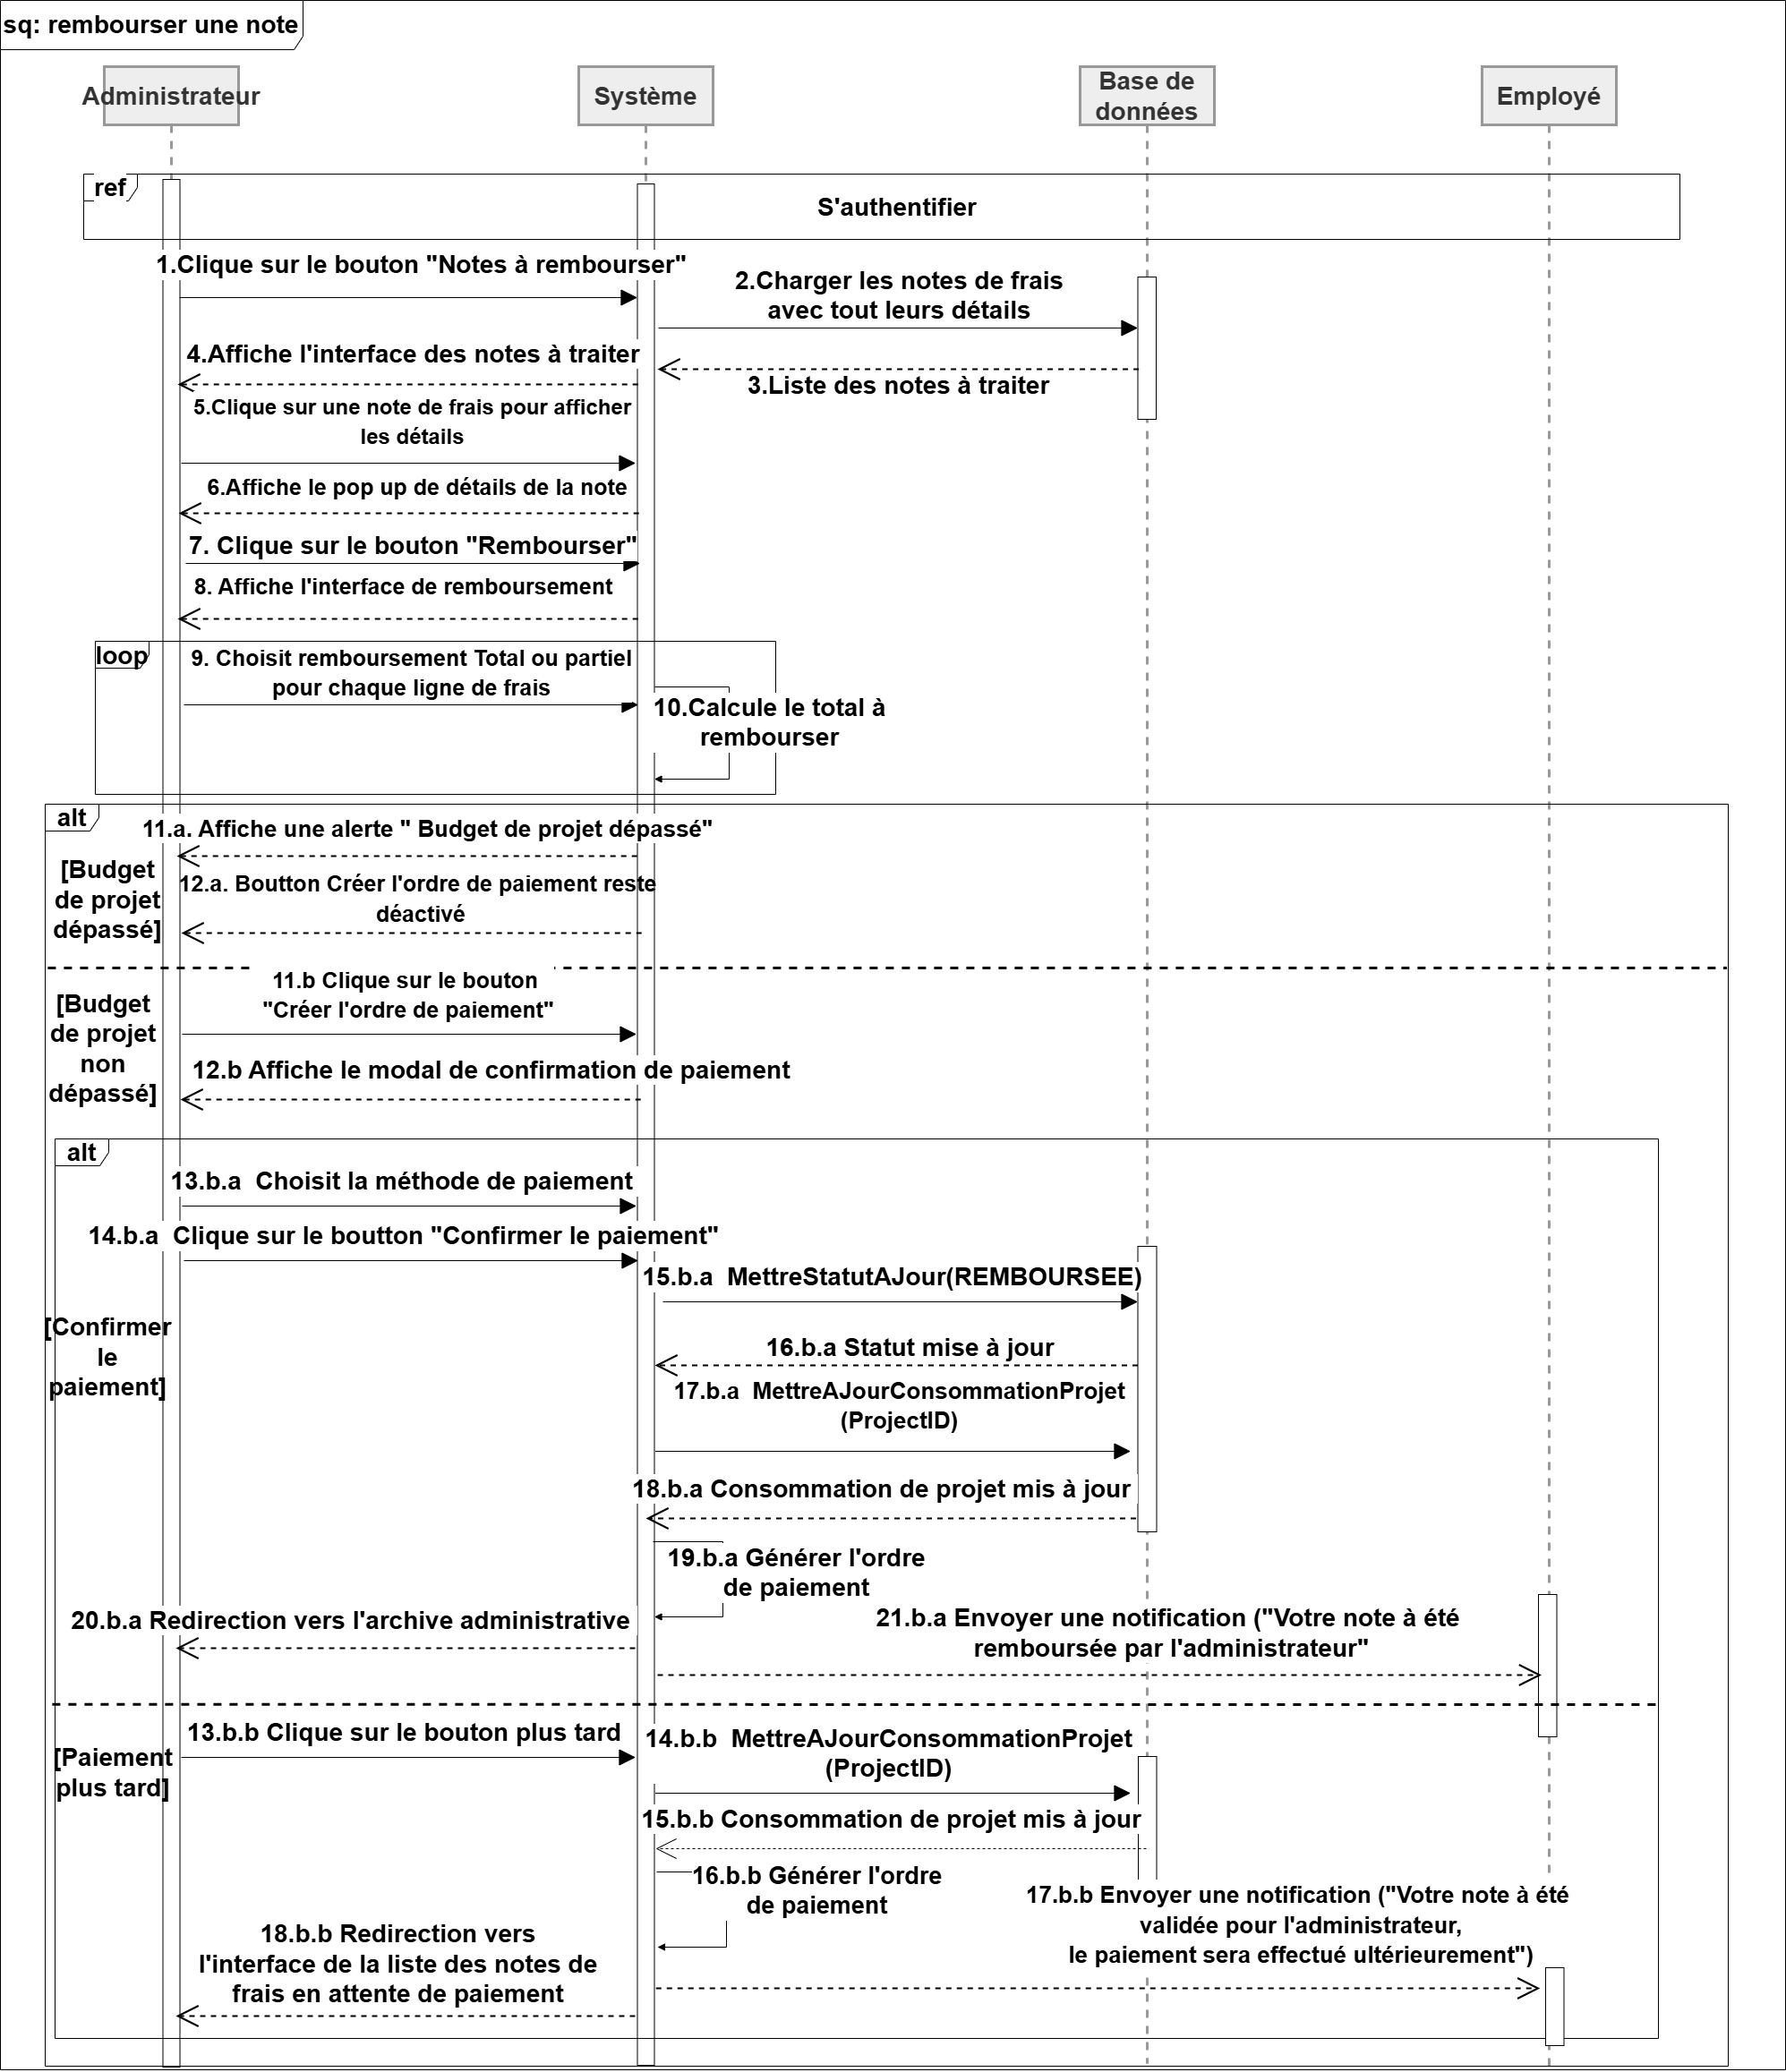
\includegraphics[width=\textwidth,height=0.86\textheight]{sequence_reimbursement.png}

\caption{Diagramme de séquence – Remboursement partiel et création d'ordre}

\label{fig:seq_partial_reimb}

\end{figure}

\subsubsection{Diagramme de séquence – Rejeter une note de frais}



\begin{figure}[H]

\centering

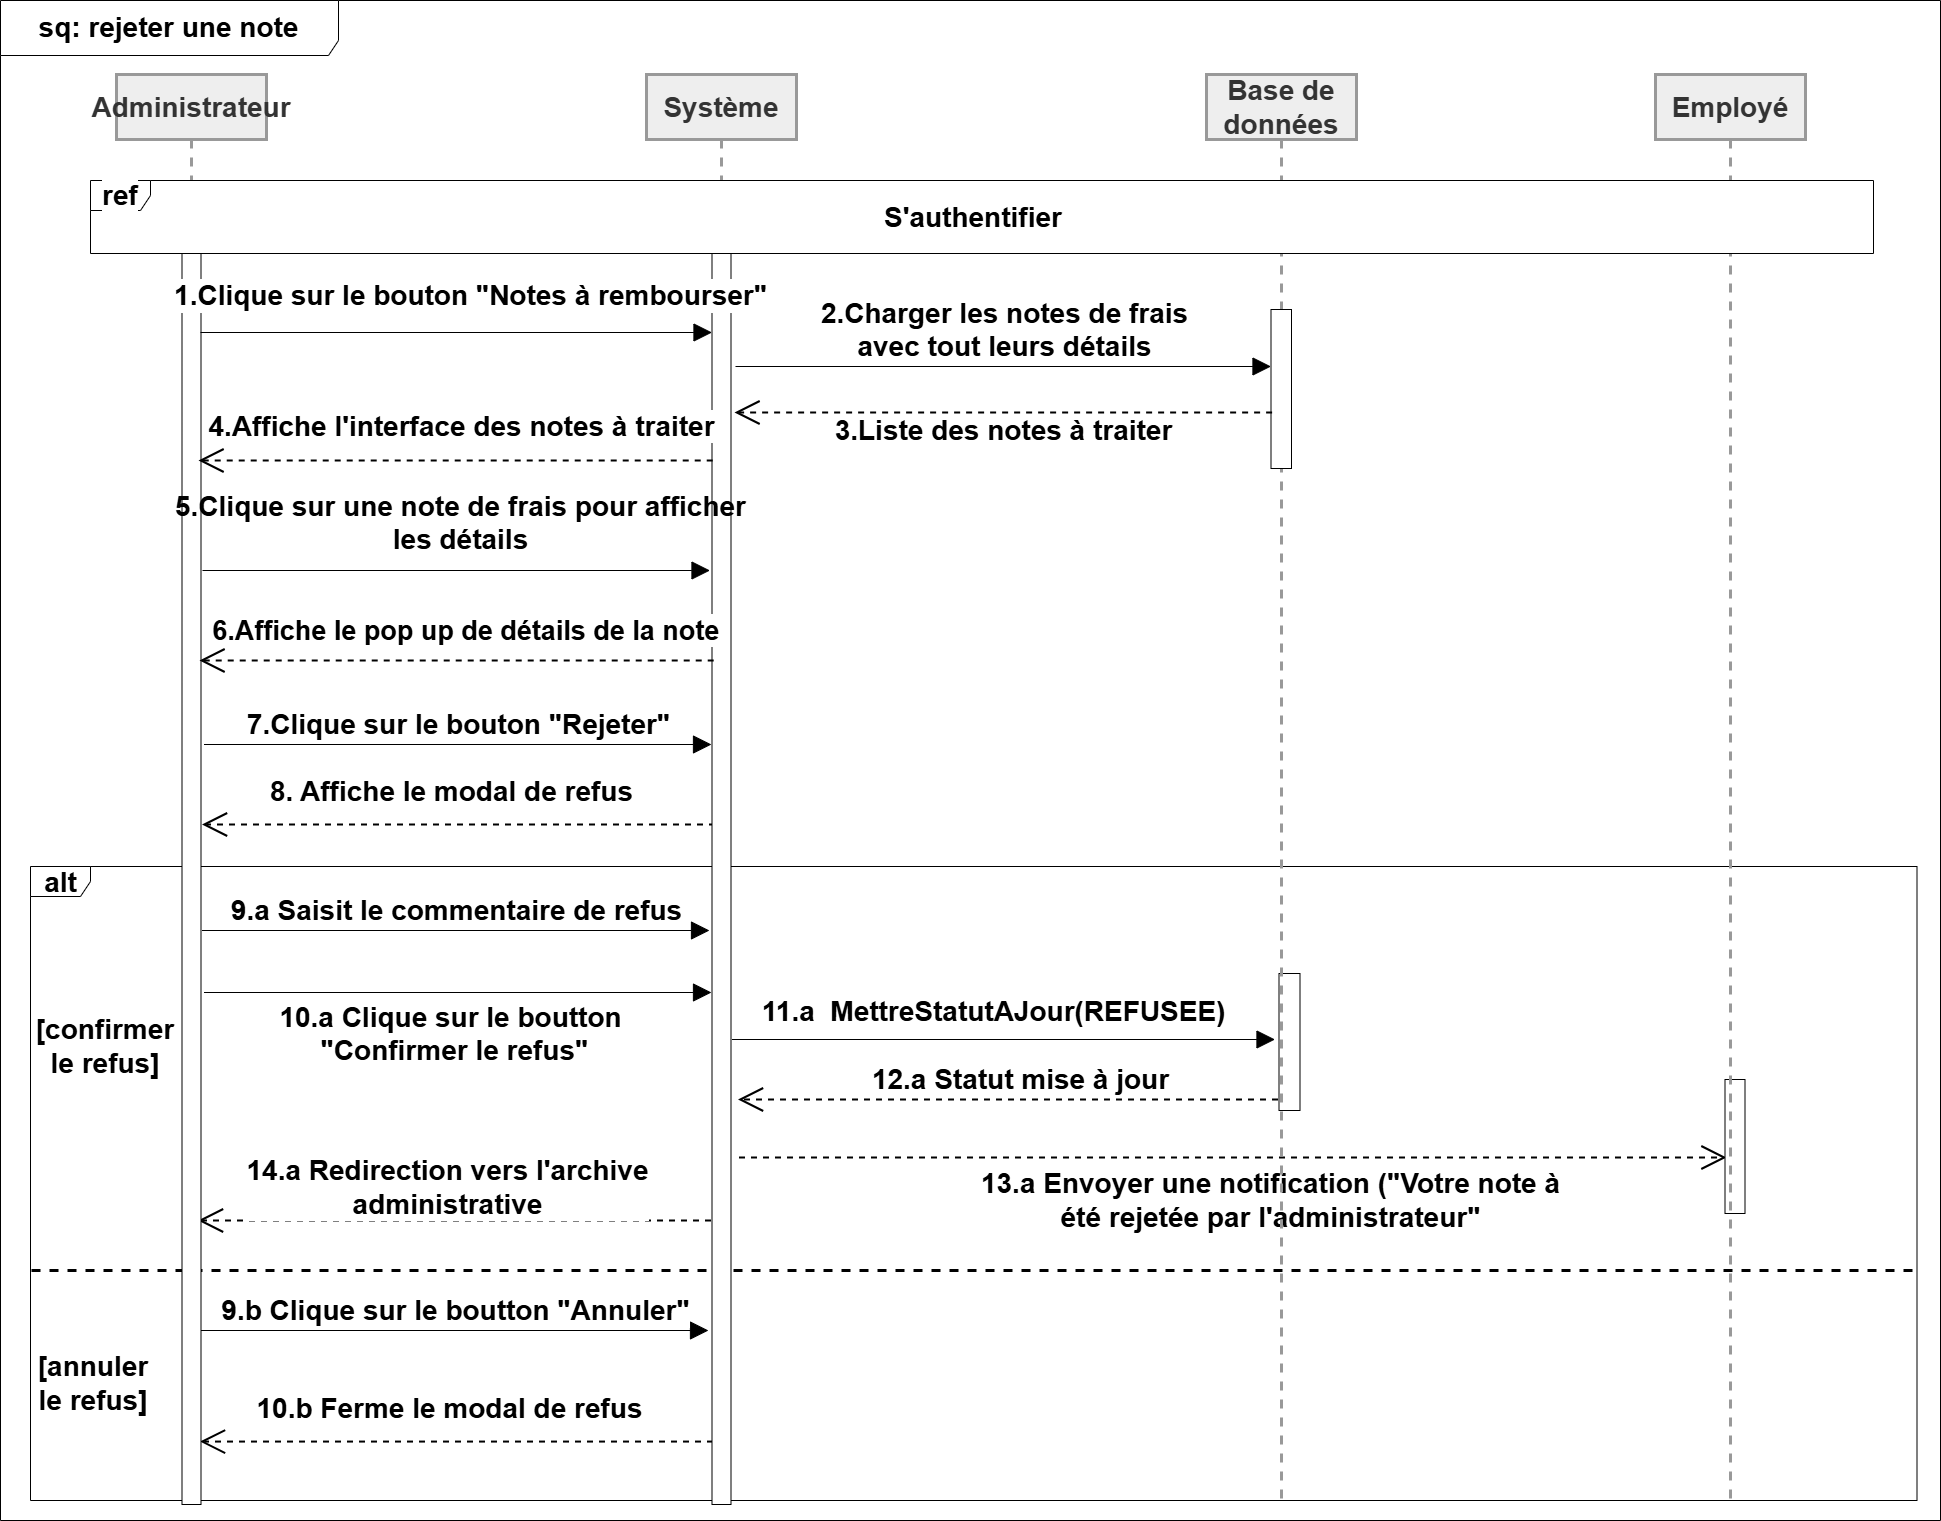
\includegraphics[width=\textwidth,height=0.7\textheight]{seq_rejection.png}

\caption{Diagramme de séquence – Rejeter une note de frais}

\label{fig:seq_rejection}

\end{figure}

\subsubsection{Diagramme de déploiement - Dockerisation}



\begin{figure}[H]

\centering

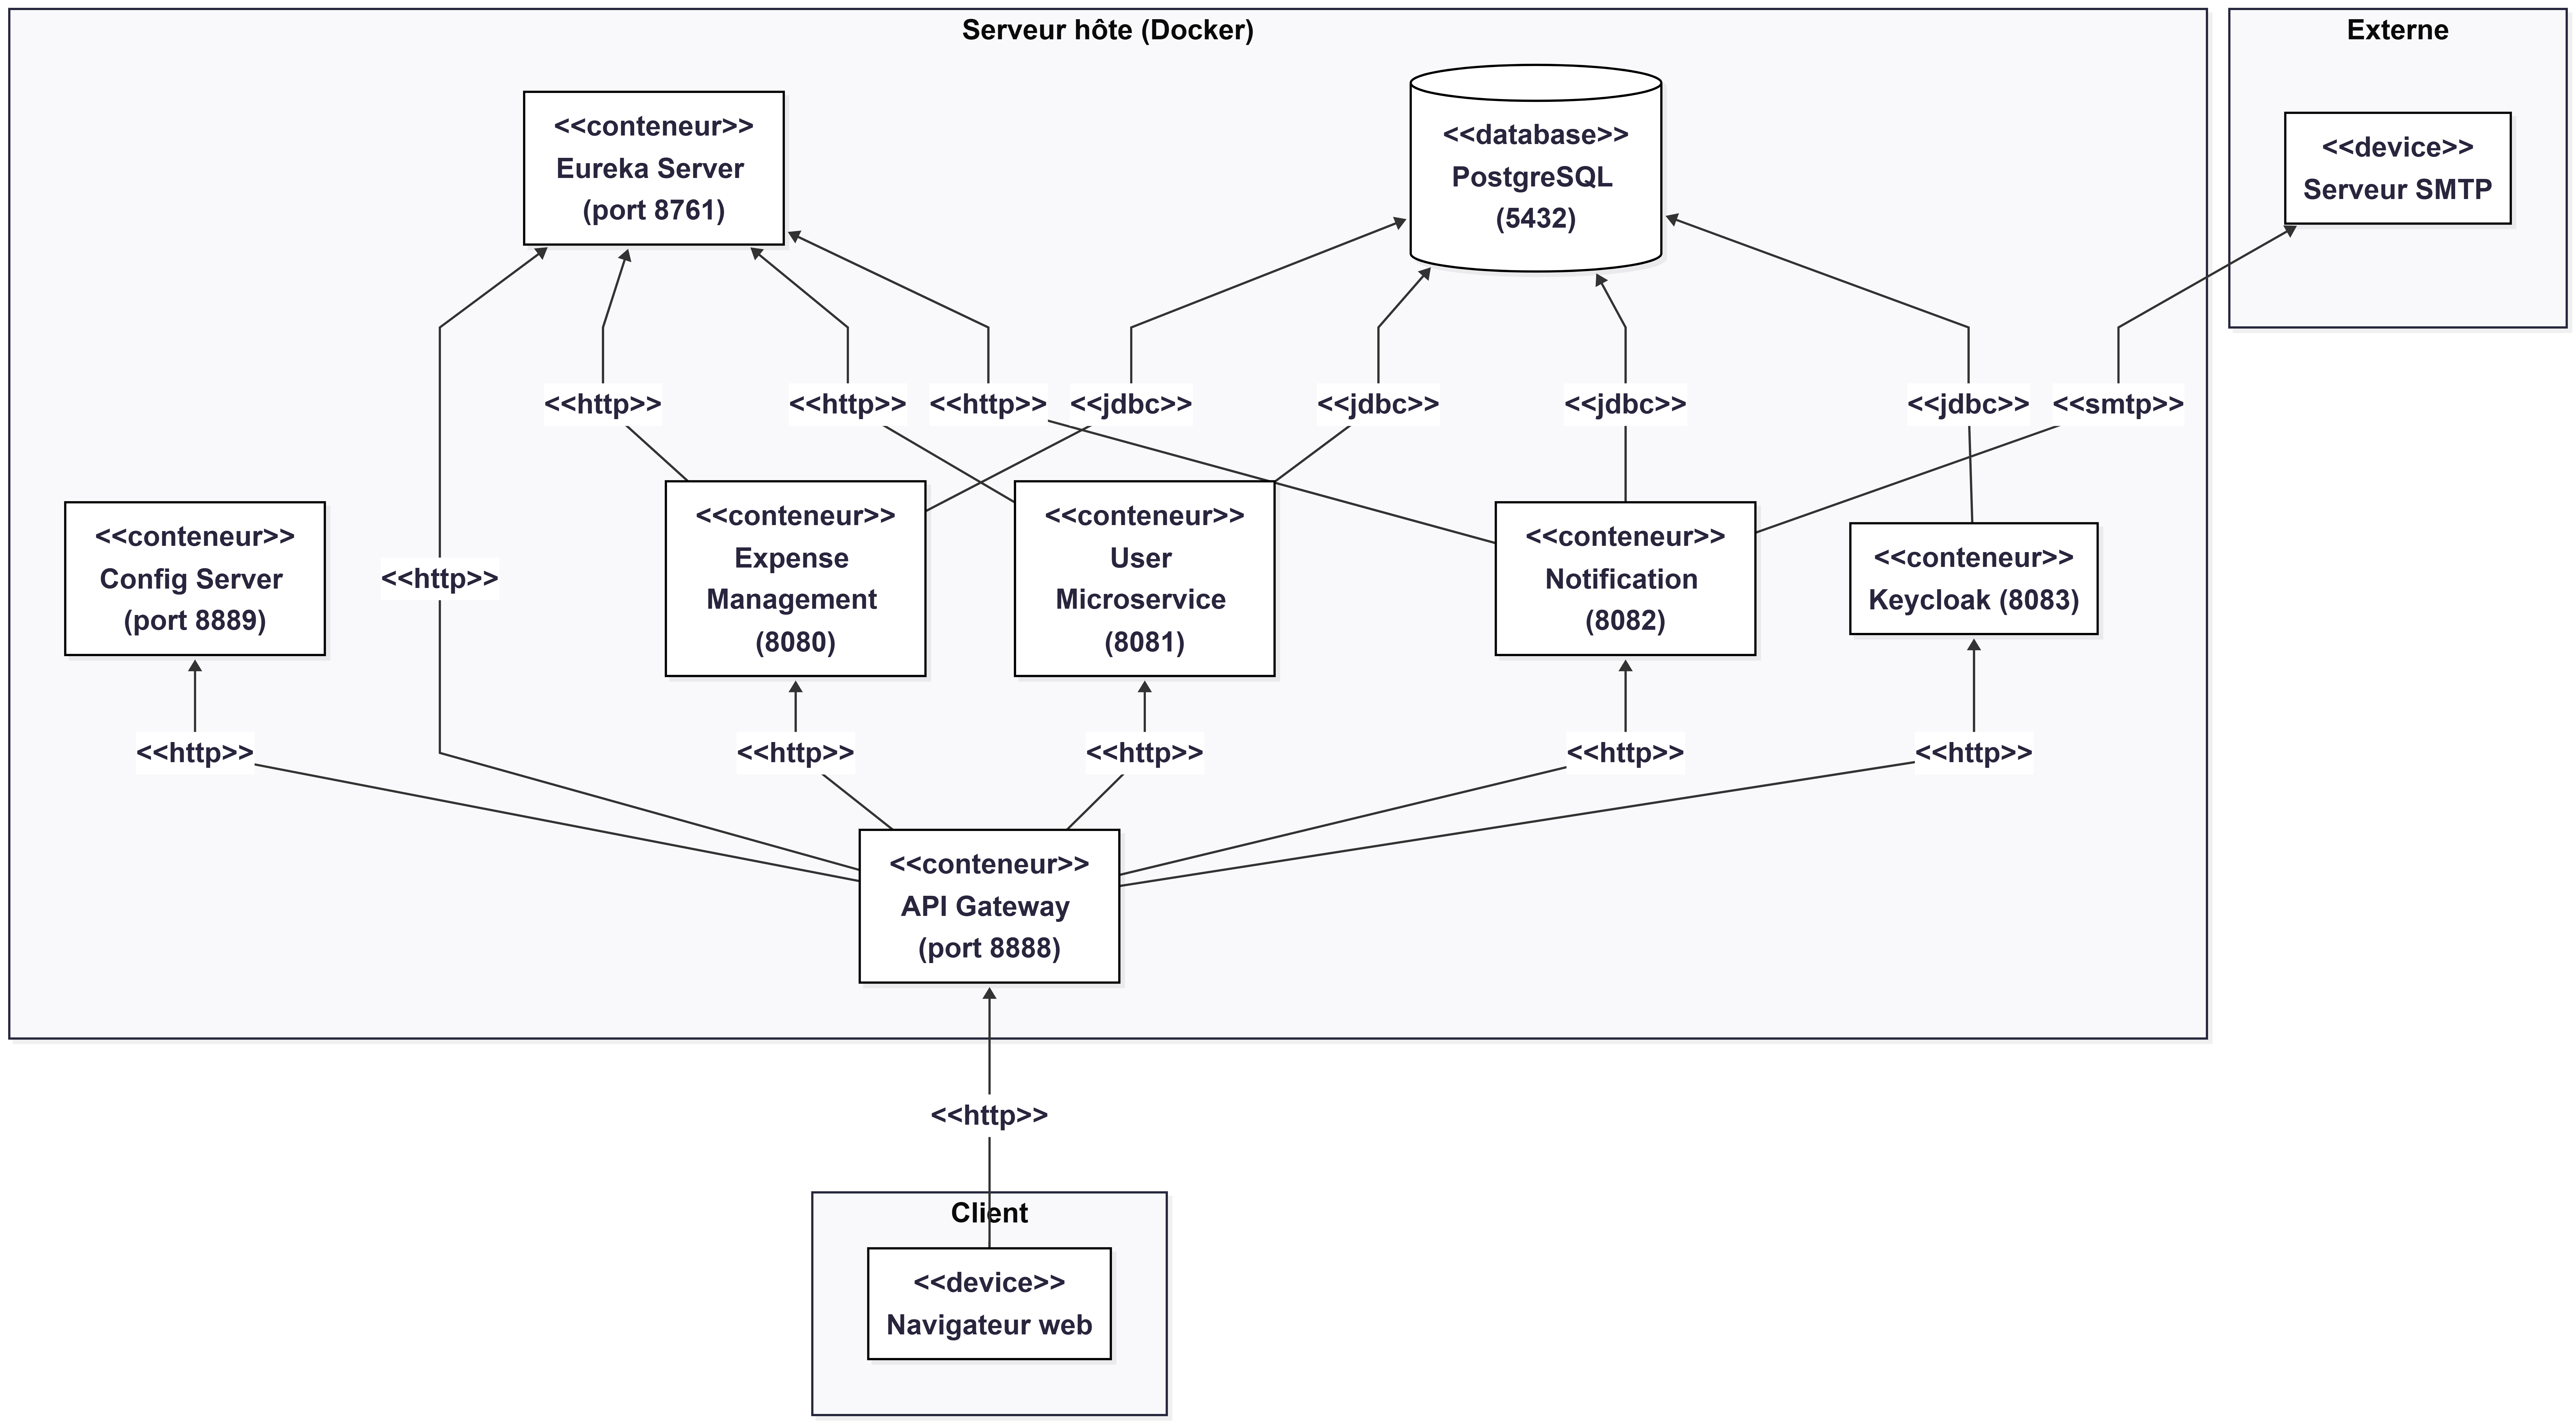
\includegraphics[width=1.2\textwidth,height=0.9\textwidth,angle=90,keepaspectratio]{deploiement_sp3.png}

\caption{Diagramme de déploiement - Docker}

\label{fig:déploiement_sp2}

\end{figure}



\subsection{Diagramme de classes du sprint 3}



\begin{figure}[H]

\centering

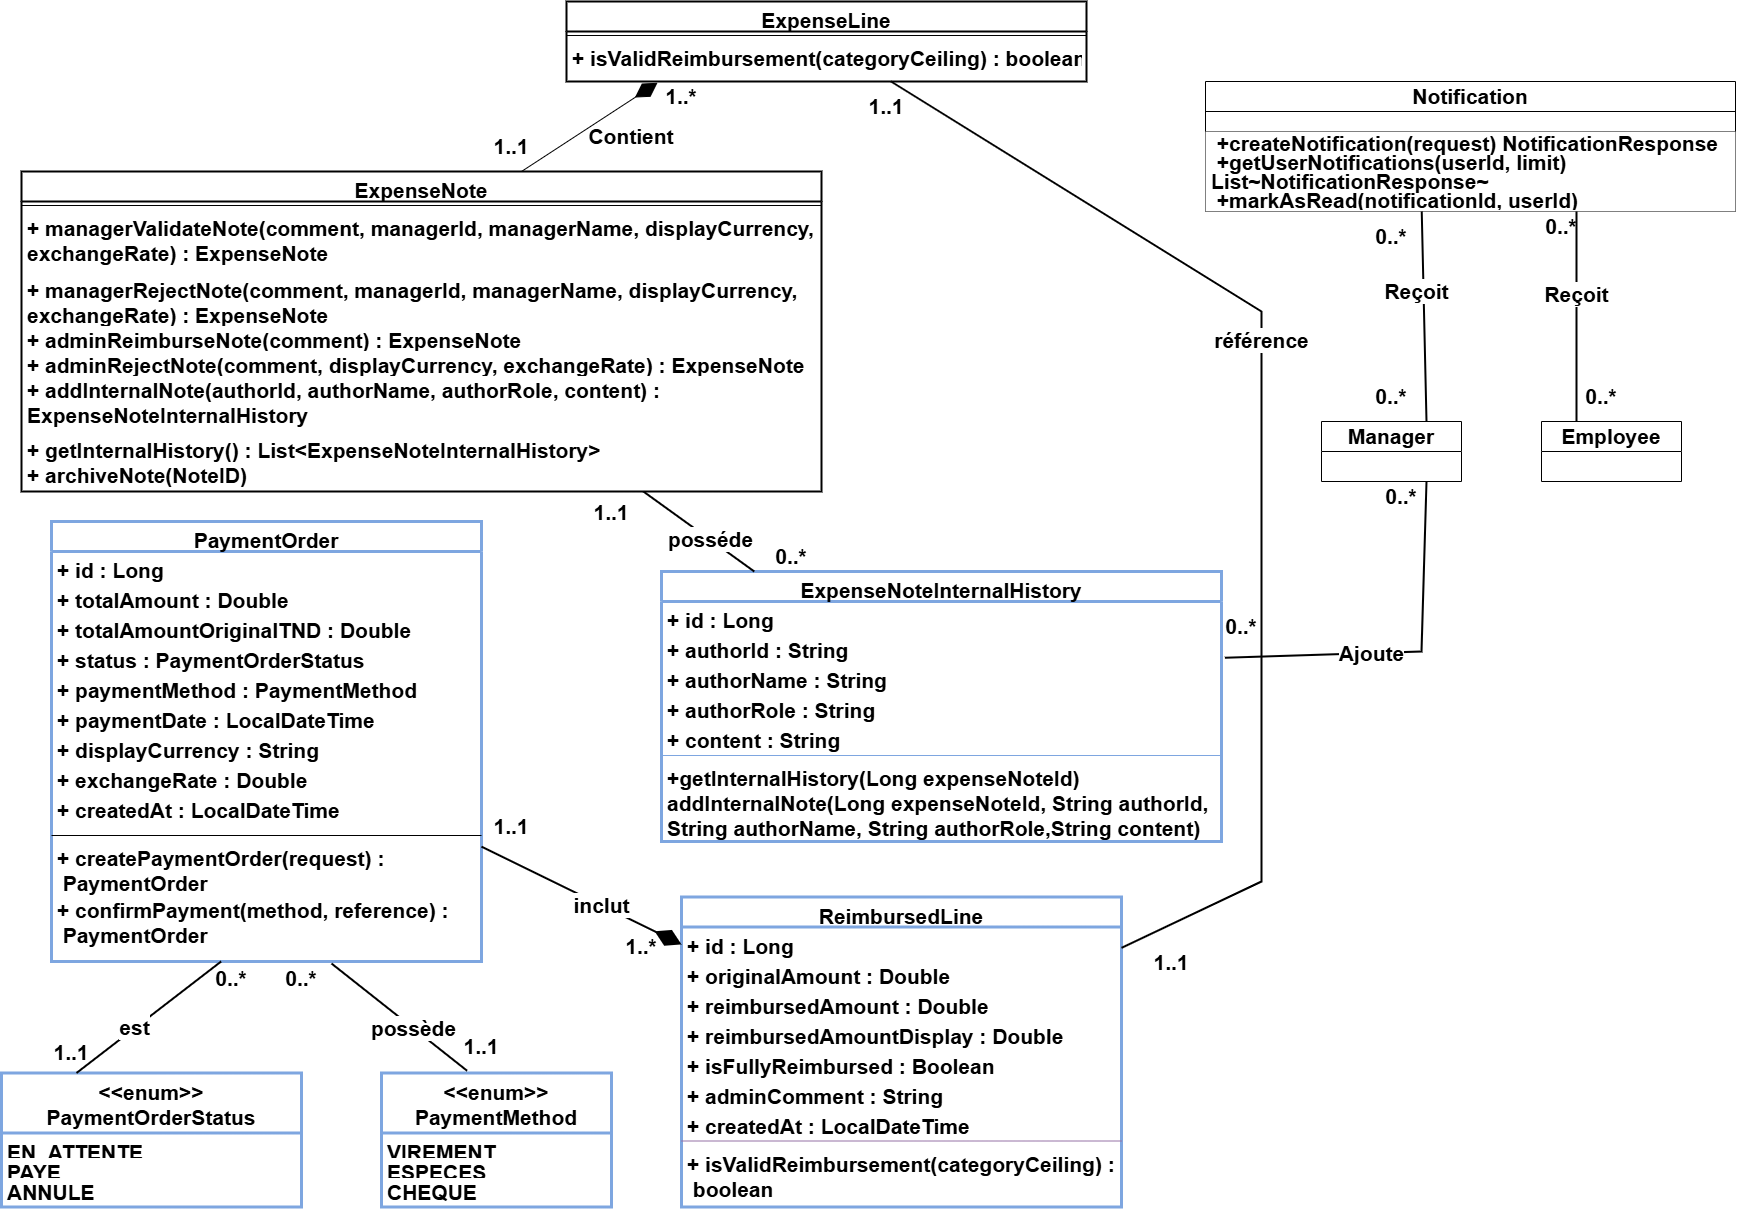
\includegraphics[width=\textwidth,height=0.65\textheight]{class_diagram_sprint3.png}

\caption{Diagramme de classes du sprint 3}

\label{fig:class_sprint3}

\end{figure}







\section{Interfaces développées}



\subsection{Liste des notes validées (page administrateur)}

Cette page permet à l’administrateur de consulter toutes les notes de frais ayant le statut \texttt{VALIDEE} par le manager, en attente de remboursement. Un tableau présente les notes avec des colonnes : numéro, employé, projet, montant total, date de validation et statut. L’administrateur peut filtrer les notes par employé, projet ou période. Chaque ligne dispose d’un bouton pour ouvrir le formulaire de remboursement ou refuser la note.



\begin{figure}[H]

 \centering

 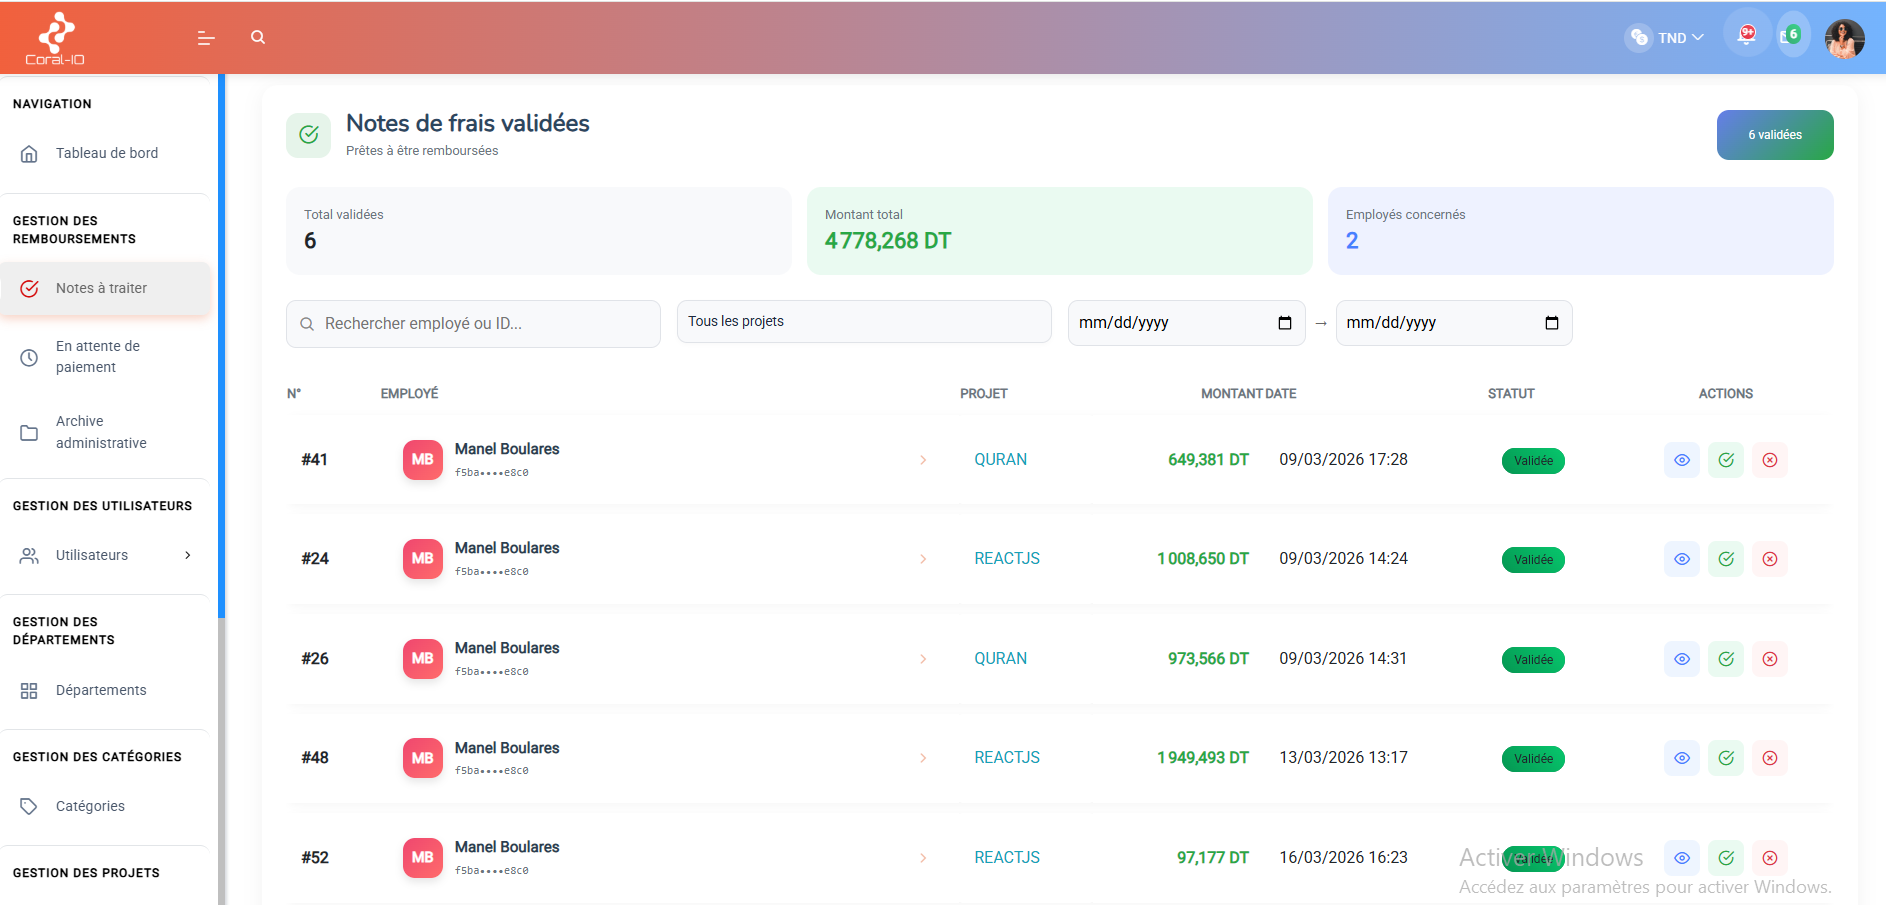
\includegraphics[width=\textwidth]{validated_notes.png}

 \caption{Liste des notes validées en attente de remboursement}

 \label{fig:validated_notes_list}

\end{figure}



\subsection{Formulaire de remboursement (administrateur)}

Ce composant permet à l’administrateur de définir les montants à rembourser ligne par ligne. Il charge la note, ses lignes de frais et les limites de remboursement (plafonds des catégories, budget restant du projet). L’utilisateur peut ajuster chaque montant, ajouter un commentaire et visualiser le total calculé dynamiquement. Un bouton « Créer l’ordre de paiement » est actif si au moins une ligne a un montant > 0 ; sinon, un bouton « Refuser (aucun remboursement) » s’affiche. Une alerte s’affiche si le montant à rembourser dépasse le budget restant du projet.



\begin{figure}[H]

 \centering

 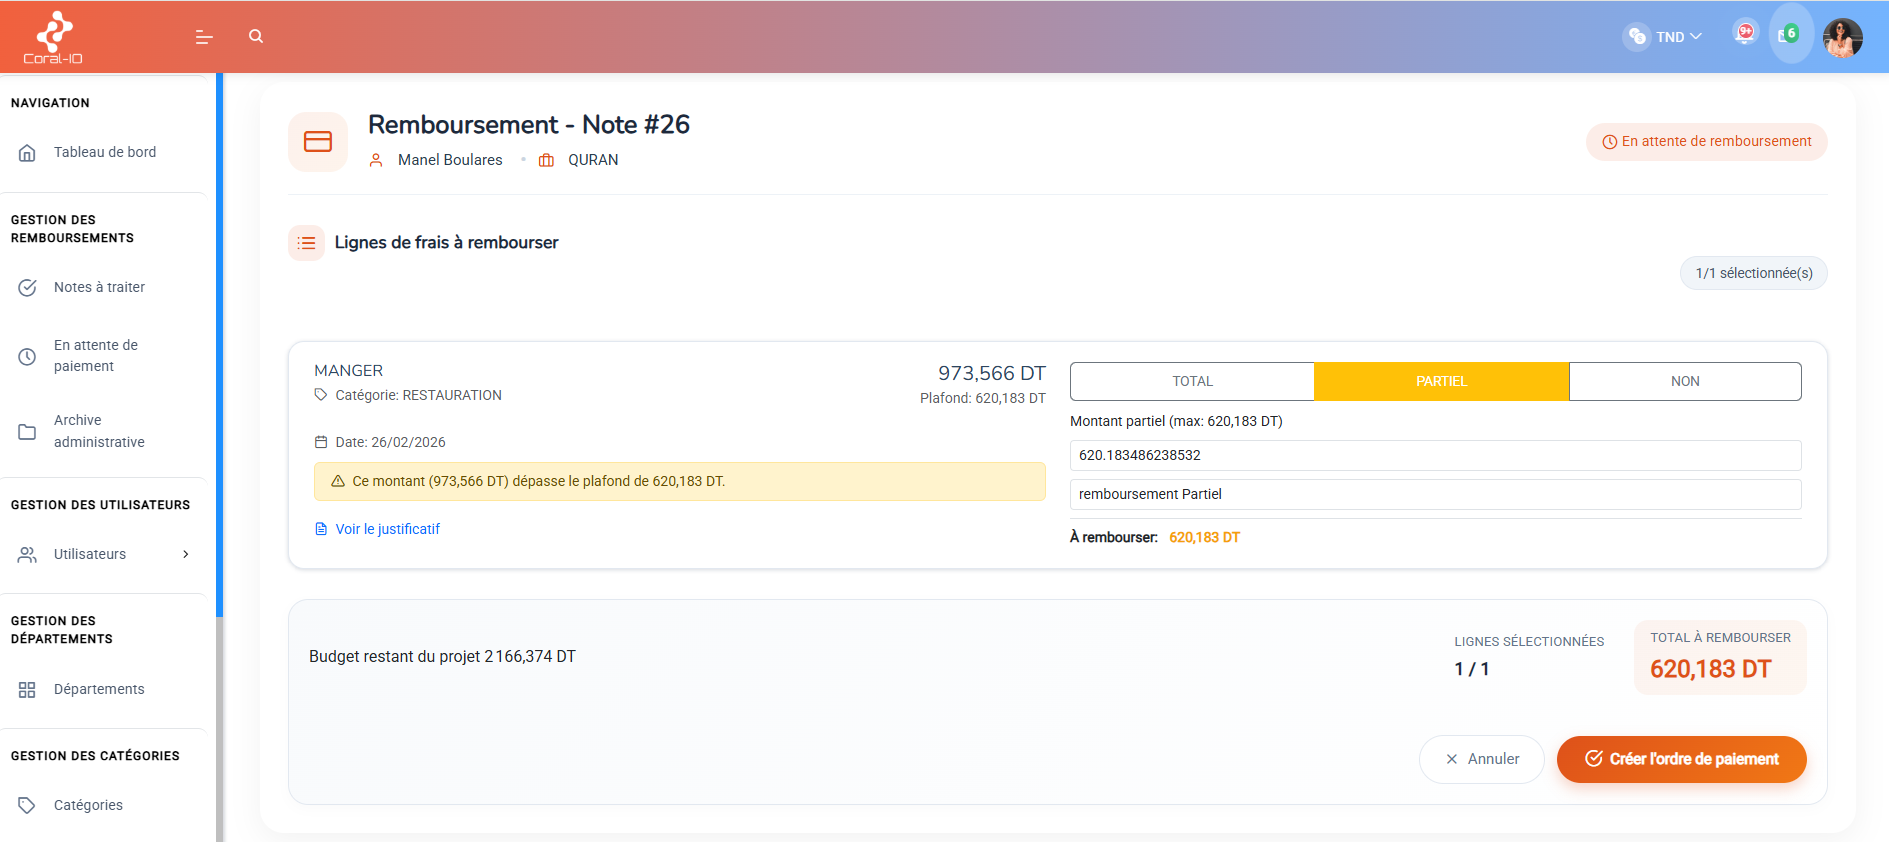
\includegraphics[width=\textwidth]{reimbursement_form.png}

 \caption{Formulaire de remboursement (total ou partiel)}

 \label{fig:reimbursement_form}

\end{figure}



\subsection{Page des ordres de paiement en attente}

Cette page liste tous les ordres de paiement avec le statut \texttt{EN\_ATTENTE}. Chaque ligne affiche le numéro de l’ordre, l’employé concerné, le montant total, la date de création et un bouton pour télécharger le PDF de l’ordre. Un clic sur une ligne permet d’accéder à la page de détail de l’ordre pour confirmer le paiement. Des filtres par employé, période et recherche textuelle sont disponibles.



\begin{figure}[H]

 \centering

 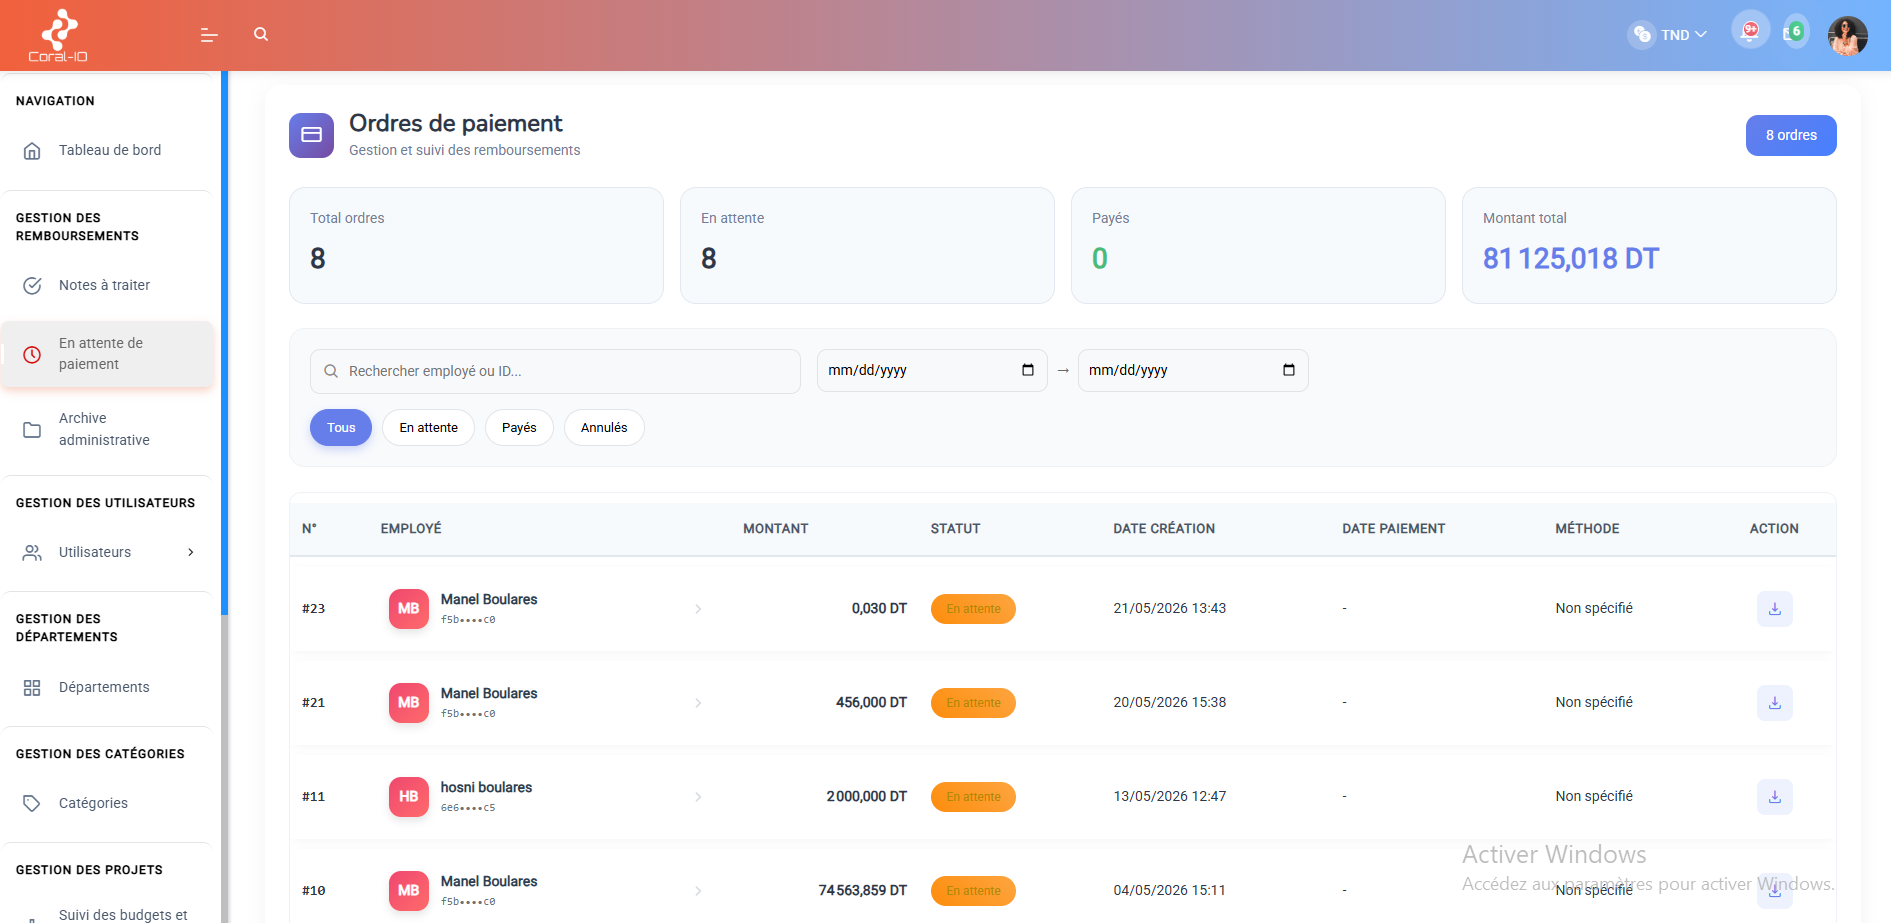
\includegraphics[width=\textwidth]{reimbursement_list.png}

 \caption{Liste des ordres de paiement en attente}

 \label{fig:reimbursement_list}

\end{figure}



\subsection{Page de détail d’un ordre de paiement}

Cette page affiche toutes les informations d’un ordre de paiement :

\begin{itemize}

 \item Informations générales : numéro d’ordre, note associée, employé, montant total, statut.

 \item Tableau détaillant chaque ligne de frais avec le montant original, le montant remboursé, le type de remboursement (total/partiel/non) et le commentaire de l’administrateur.

 \item Section « Informations de paiement » : méthode de paiement, référence et date (si déjà payé).

 \item Actions possibles selon le statut : bouton « Confirmer le paiement » (si \texttt{EN\_ATTENTE}) ou bouton retour à l’archive (si \texttt{PAYE} ou \texttt{ANNULE}).

 \item Bouton de téléchargement du PDF de l’ordre.

\end{itemize}



\begin{figure}[H]

 \centering

 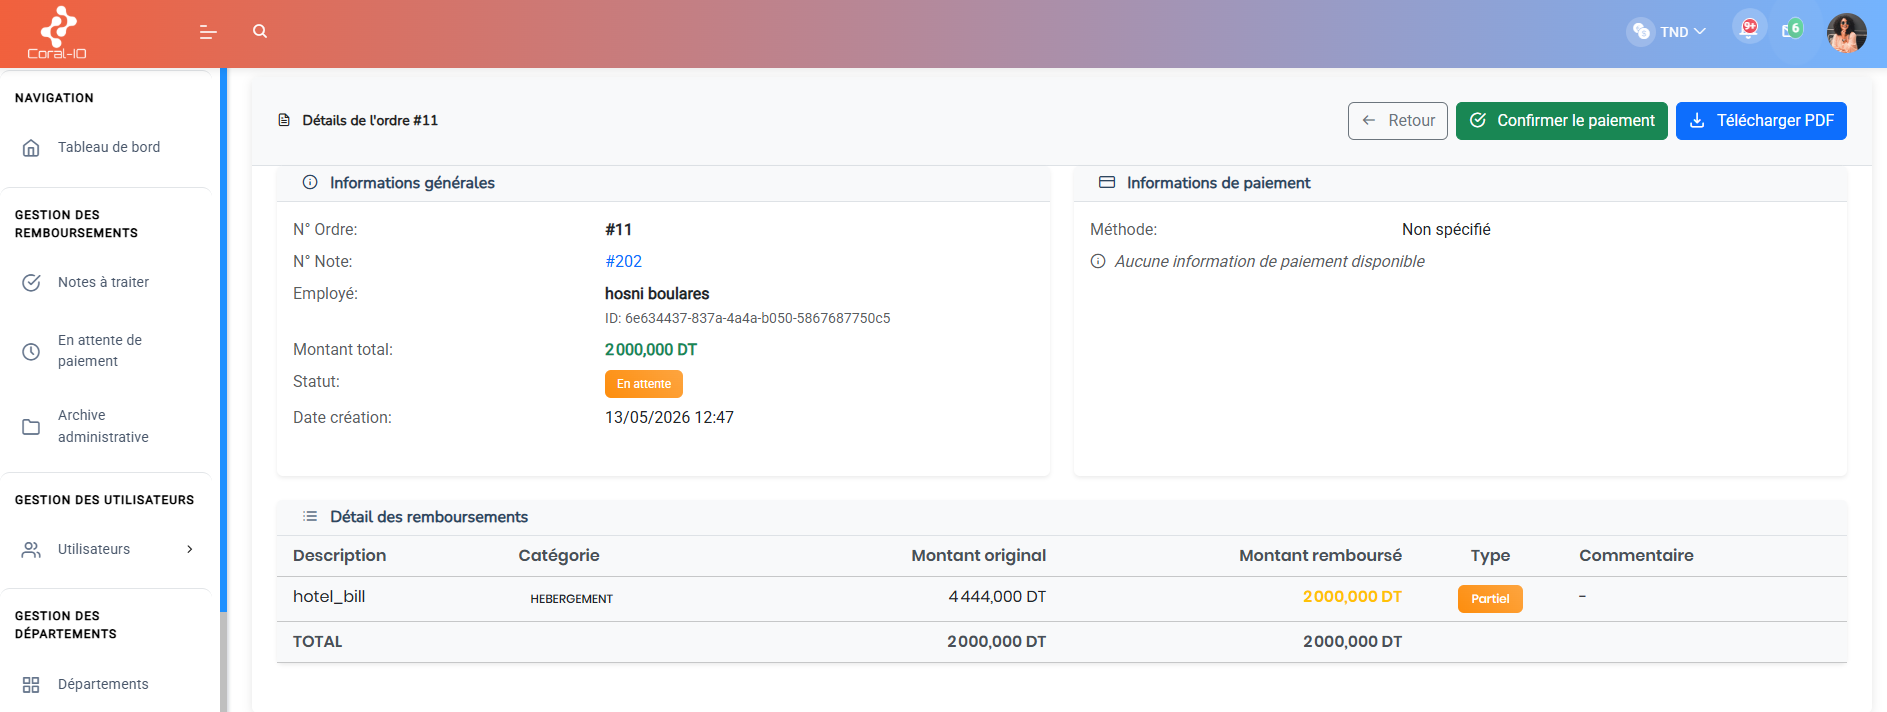
\includegraphics[width=\textwidth]{order_details.png}

 \caption{Détail d’un ordre de paiement}

 \label{fig:order_details}

\end{figure}



\subsection{Modal de confirmation de paiement}

Ce modal s’ouvre lorsque l’administrateur clique sur « Confirmer le paiement » dans la page de détail d’un ordre. Il contient un sélecteur de méthode de paiement (virement bancaire, chèque, espèces), un champ optionnel pour une référence (numéro de virement, numéro de chèque) et les boutons « Confirmer » et « Annuler ». Après confirmation, l’ordre passe en statut \texttt{PAYE} et la note associée est mise à jour en \texttt{REMBOURSEE}.



\begin{figure}[H]

 \centering

 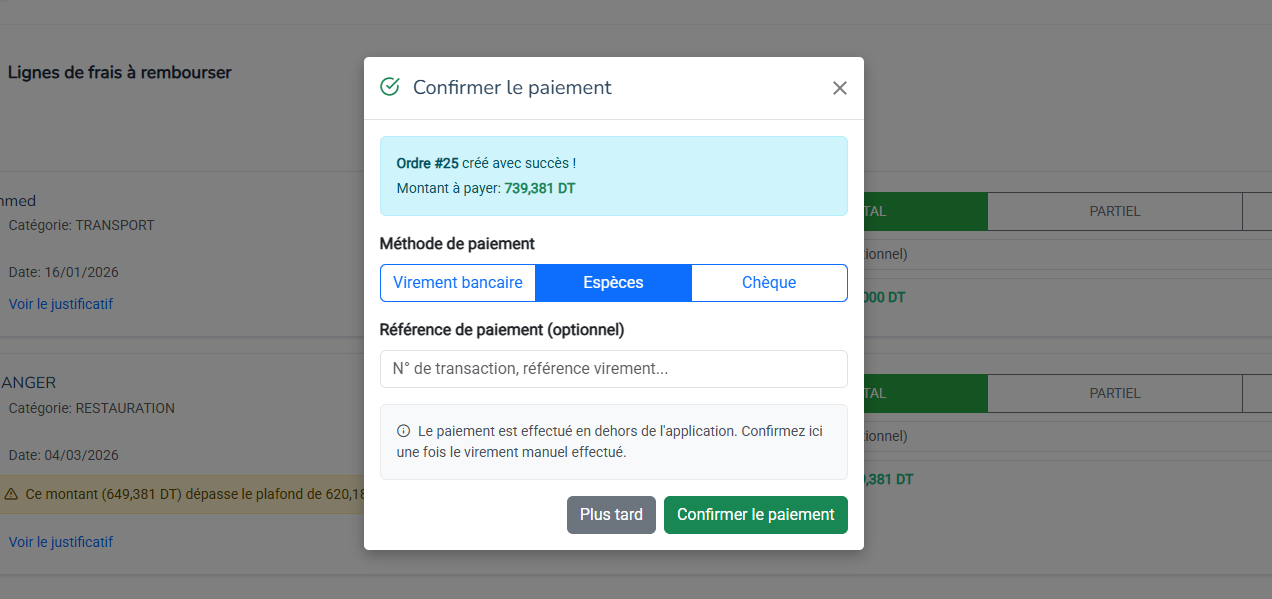
\includegraphics[width=\textwidth]{payment_confirmation_modal.png}

 \caption{Modal de confirmation de paiement}

 \label{fig:payment_confirmation_modal}

\end{figure}



\subsection{Modal de confirmation de refus de remboursement}

Ce modal s’ouvre lorsque l’administrateur clique sur « Refuser » une note validée. Il affiche les informations de la note (numéro, employé, montant total) et un texte d’avertissement indiquant que l’action est irréversible et qu’une notification sera envoyée à l’employé et au manager. Un champ de commentaire obligatoire permet de justifier le refus. Les boutons « Confirmer le refus » et « Annuler » sont présents, avec un état de chargement pendant le traitement.



\begin{figure}[H]

 \centering

 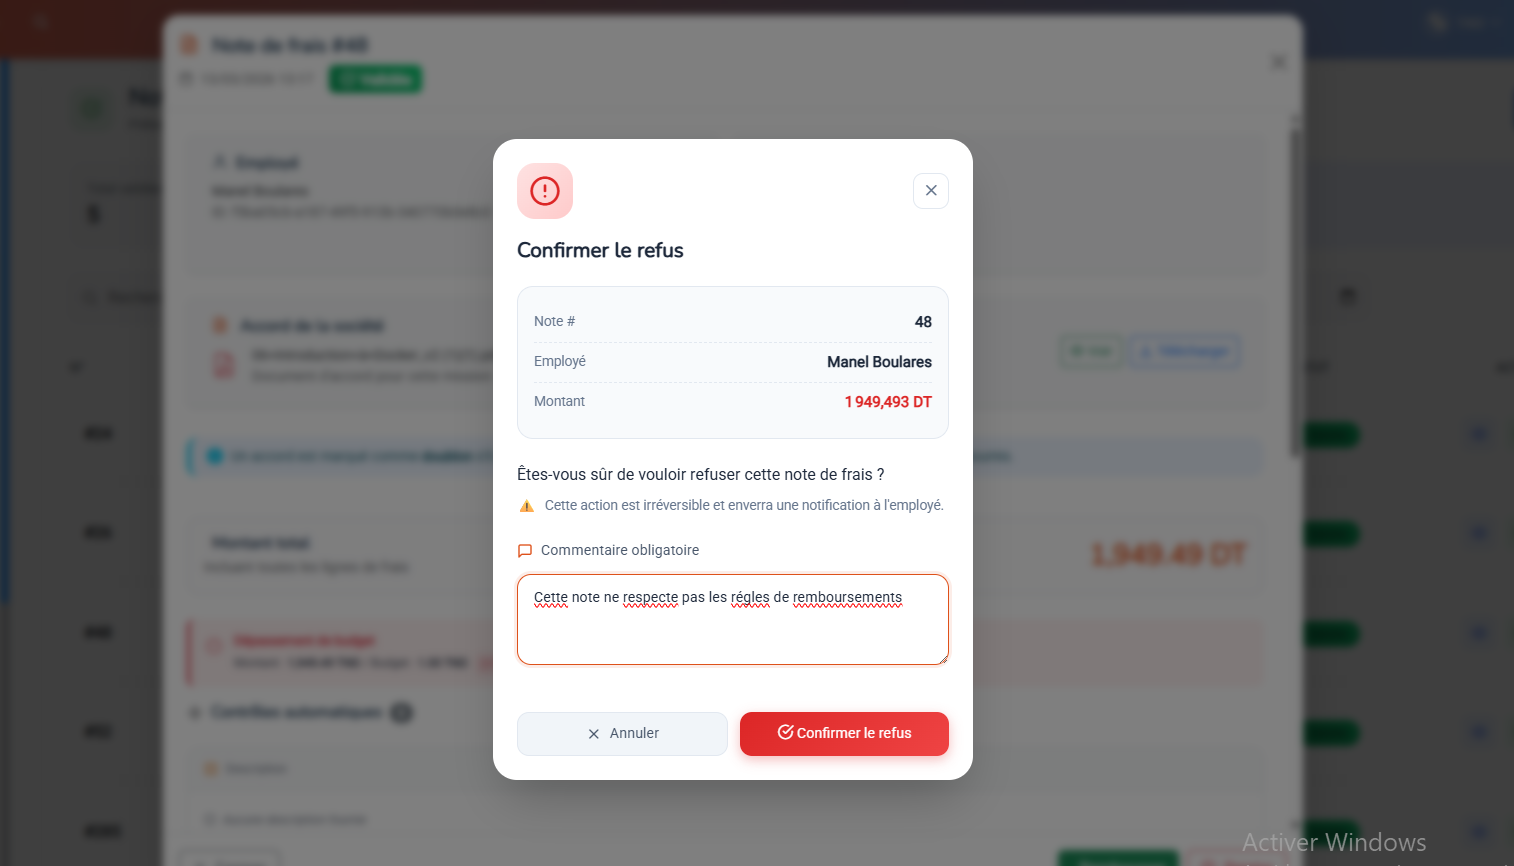
\includegraphics[width=\textwidth]{reject_modal.png}

 \caption{Modal de confirmation de refus de remboursement}

 \label{fig:reject_modal}

\end{figure}



\subsection{Page d’archive administrative}

Cette page consolide deux types d’éléments :

\begin{itemize}

 \item Les ordres de paiement avec statut \texttt{PAYE} ou \texttt{ANNULE}.

 \item Les notes de frais ayant le statut \texttt{REFUSEE} (rejetées par l’administrateur ou par le manager).

\end{itemize}

Pour chaque élément, on affiche le type (Ordre / Note), la référence, l’employé, le projet, le montant, le statut (avec badge de couleur), un indicateur de remboursement complet/partiel (pour les ordres payés), la décision (qui a pris la décision et commentaire éventuel) et des actions (voir la note originale, télécharger le PDF pour les ordres). Des filtres puissants permettent de rechercher par employé, projet, type, statut, date, et type de remboursement.



\begin{figure}[H]

 \centering

 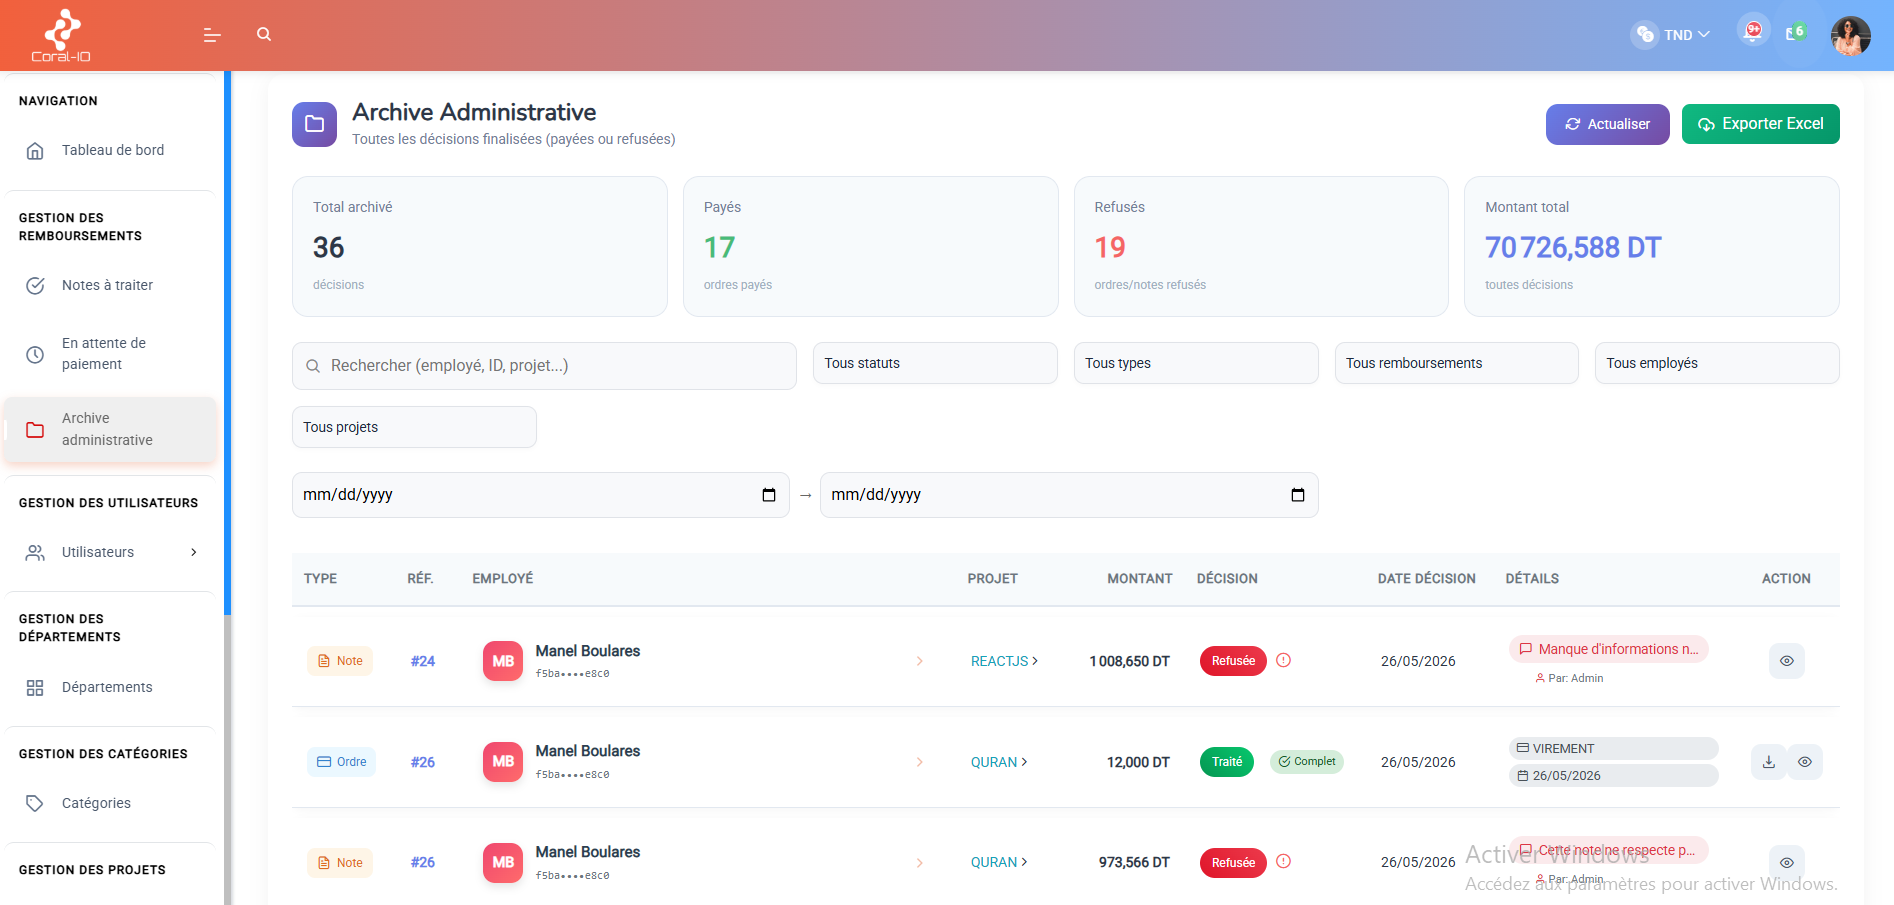
\includegraphics[width=\textwidth]{archive_page.png}

 \caption{Archive administrative consolidée}

 \label{fig:archive_page}

\end{figure}



\subsection{Notes internes (manager et administrateur)}

Dans le popup de détail d’une note de frais, deux onglets (ou zones) distincts permettent d’ajouter des notes internes :

\begin{itemize}

 \item Le manager peut ajouter une note interne visible uniquement par l’administrateur, pour signaler un contexte particulier.

 \item L’administrateur peut ajouter une note interne visible uniquement par le manager, pour communiquer une information (retard de paiement, validation partielle, anomalie).

\end{itemize}

Chaque note interne affiche l’auteur, la date et le contenu. L’historique complet des notes internes est consultable dans le popup.



\begin{figure}[H]

 \centering

 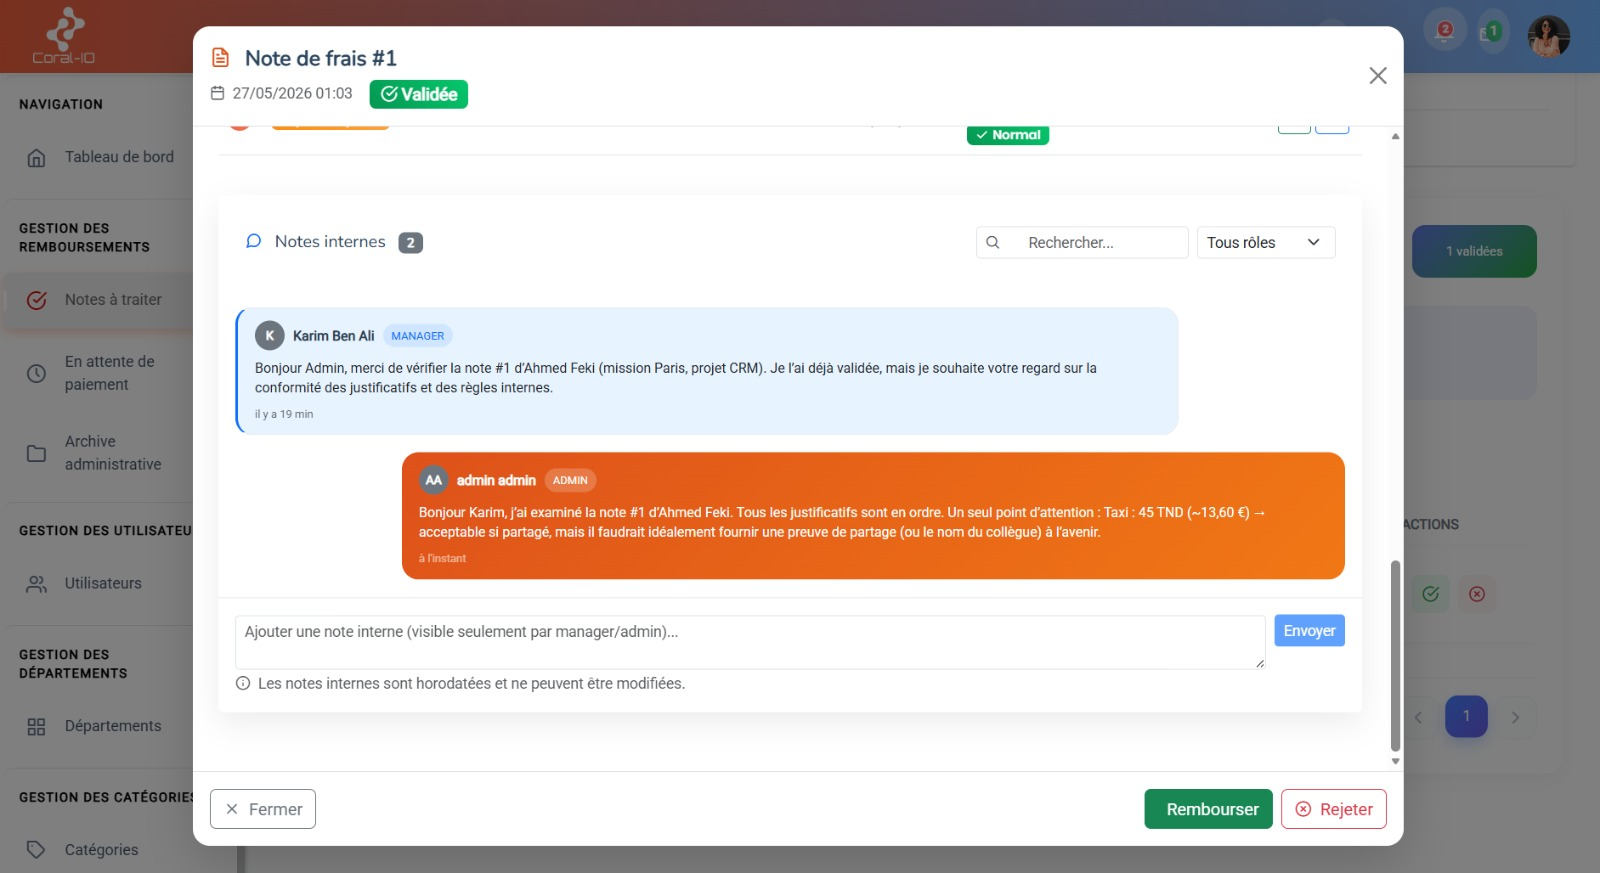
\includegraphics[width=\textwidth]{noteinterne.jpeg}

 \caption{Notes internes confidentielles dans le popup de détail}

 \label{fig:internal_notes}

\end{figure}

\begin{figure}[H]

 \centering

 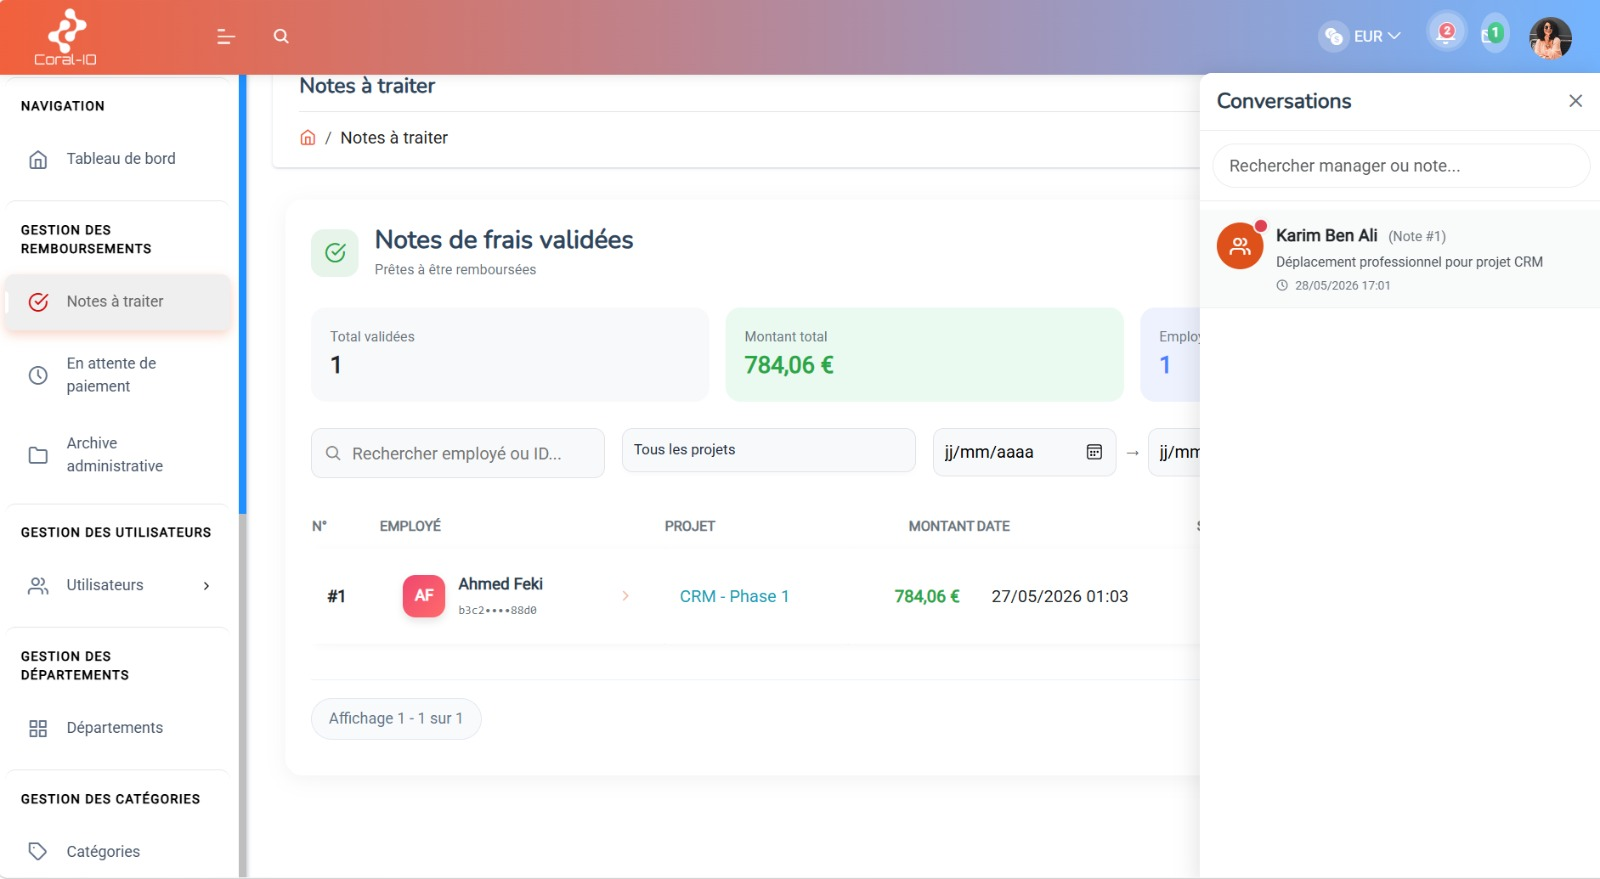
\includegraphics[width=\textwidth]{mesagerie_note_interne.jpeg}

 \caption{Liste des conversations pour messagerie des notes internes}

 \label{fig:internal_notes}

\end{figure}

\begin{figure}[H]

 \centering

 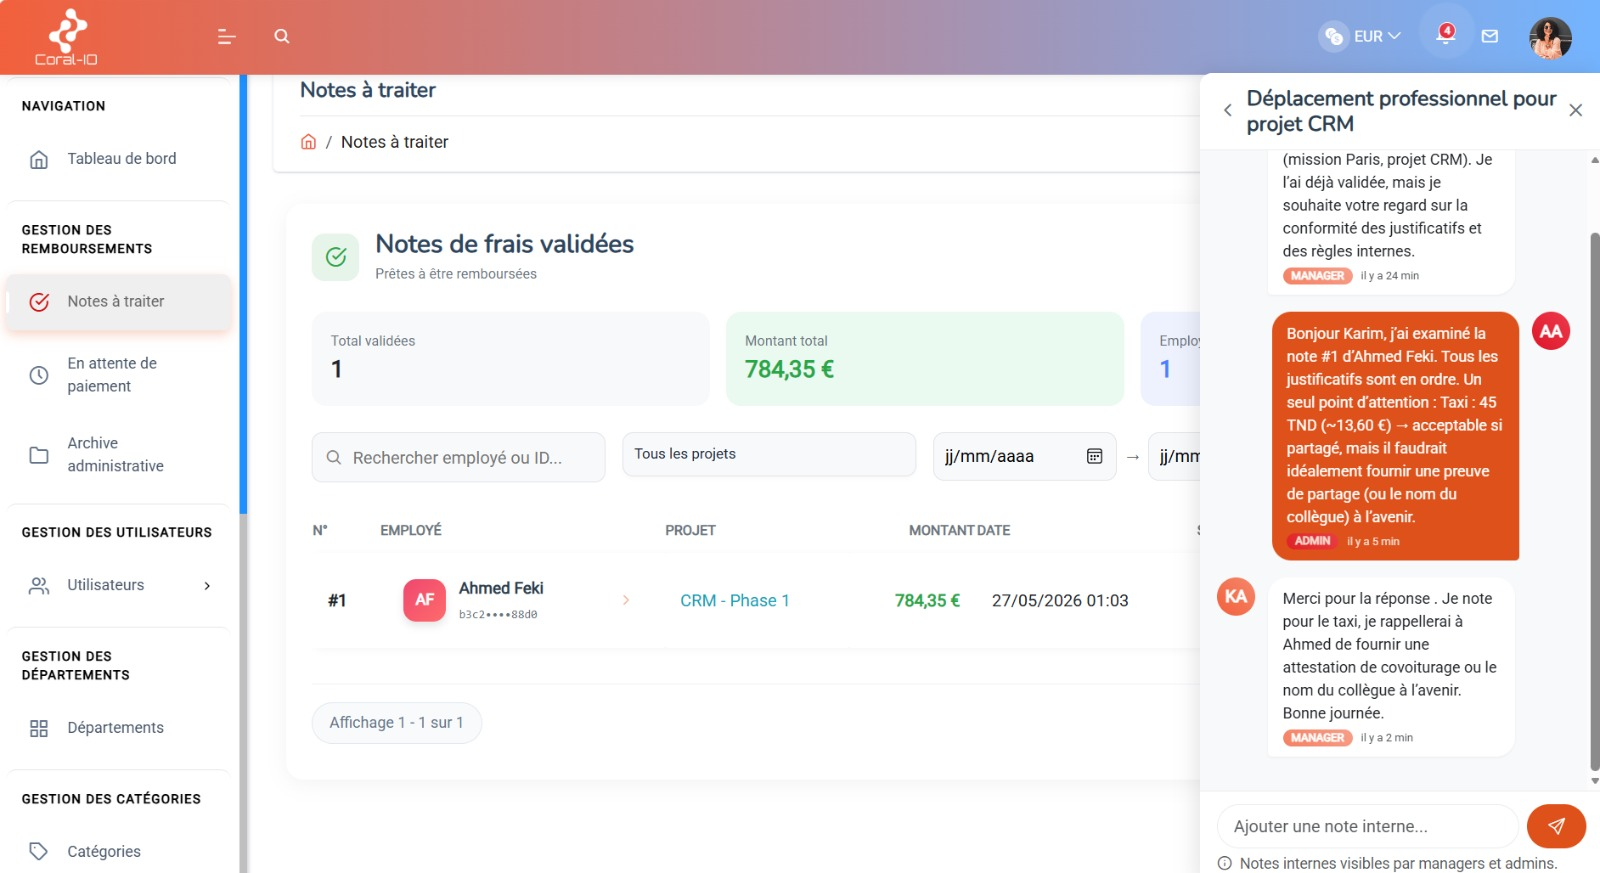
\includegraphics[width=\textwidth]{discussion_note_interne.jpeg}

 \caption{Panneau de discussion pour messagerie des notes internes}

 \label{fig:internal_notes}

\end{figure}

\subsection{Dashboard projets administrateur}

Ce tableau de bord dédié permet à l’administrateur de suivre les budgets et consommations des projets. Il offre :

\begin{itemize}

 \item Des cartes KPI : total projets, budget total, consommation totale, projets critiques.

 \item Un tableau des projets avec colonnes : ID, nom, code, statut, budget, montant consommé, reste, pourcentage d’utilisation (barre de progression colorée) et nombre d’employés affectés.

 \item Des graphiques : dépenses par catégorie (nombre et montant), comparaison budget vs dépenses (top 6 projets).

 \item Des filtres : période (aujourd’hui, semaine, mois, personnalisé), statut du projet, seuil critique, recherche textuelle.

 \item Export des données au format CSV et PDF.

\end{itemize}



\begin{figure}[H]

 \centering

 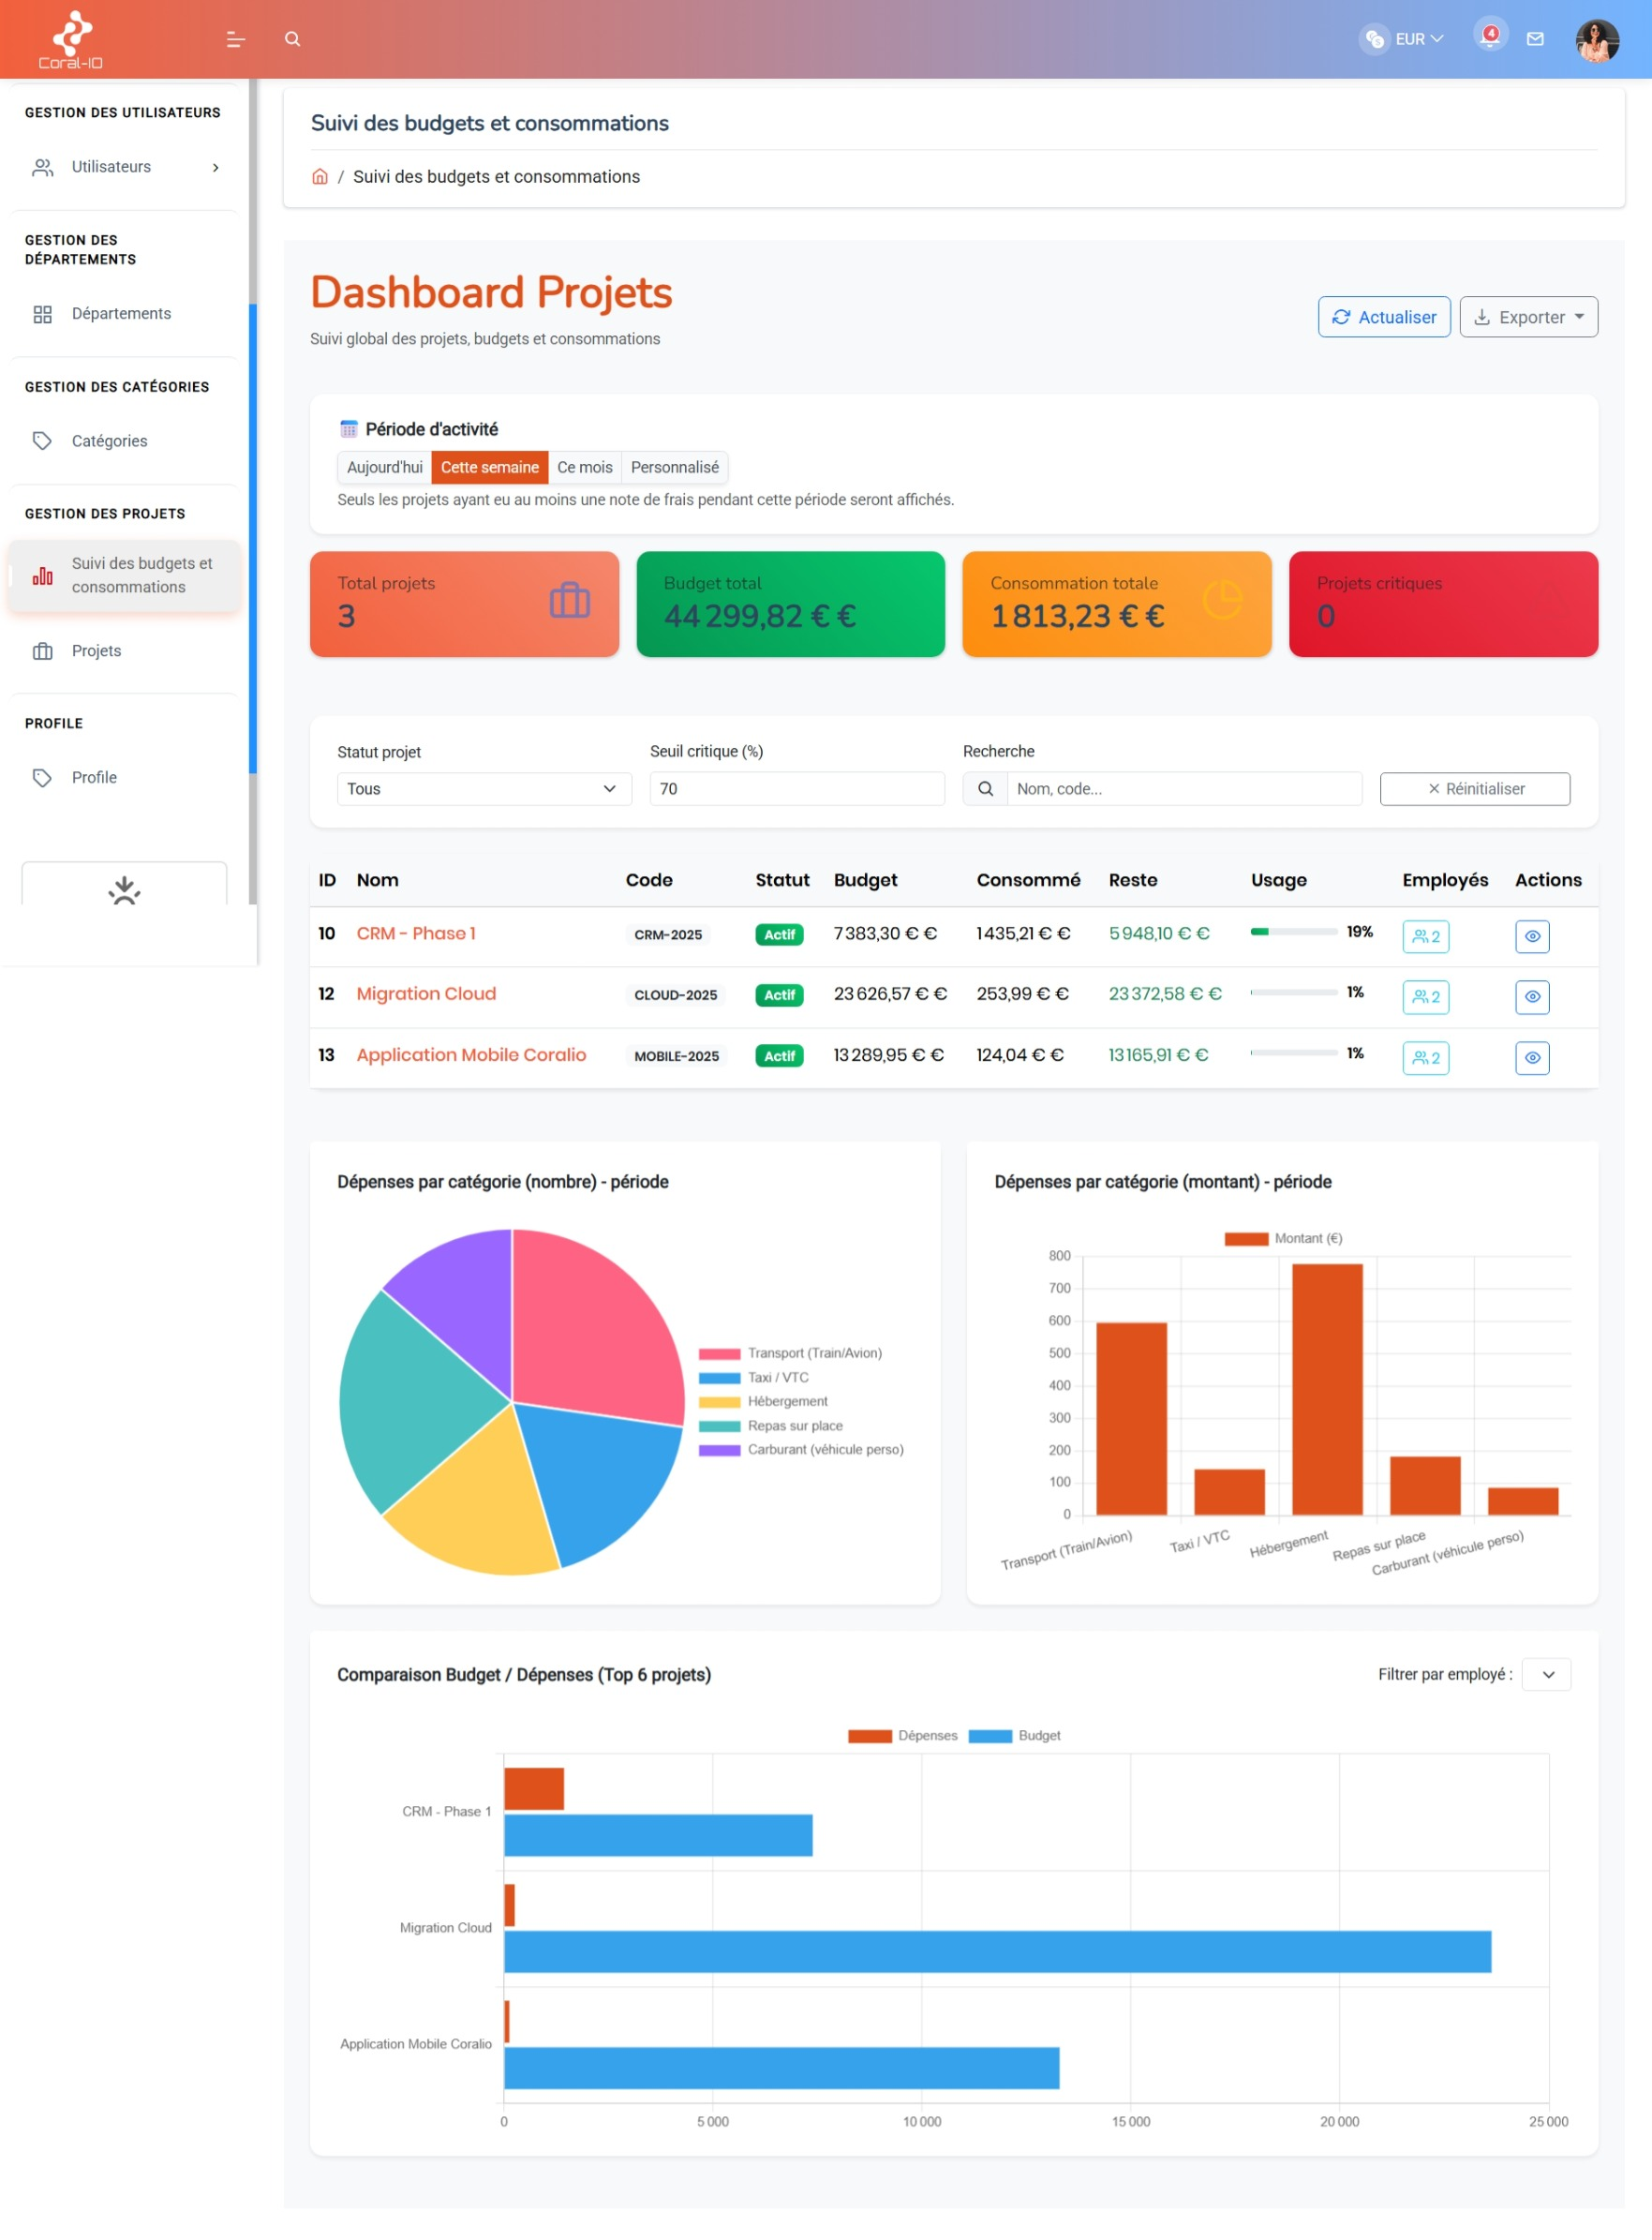
\includegraphics[width=\textwidth]{dashboard_projet.jpeg}

 \caption{Dashboard projets administrateur}

 \label{fig:admin_project_dashboard}

\end{figure}



\subsection{Export Excel/CSV}

L’administrateur peut exporter les données des tableaux (notes, projets, etc.) aux formats Excel (.xlsx) ou CSV. Un bouton « Exporter » est disponible dans les pages de liste (notes validées, archive, dashboard projets, etc.). Le fichier généré contient les colonnes affichées dans le tableau, avec les montants convertis dans la devise courante de l’utilisateur.



\begin{figure}[H]

 \centering

 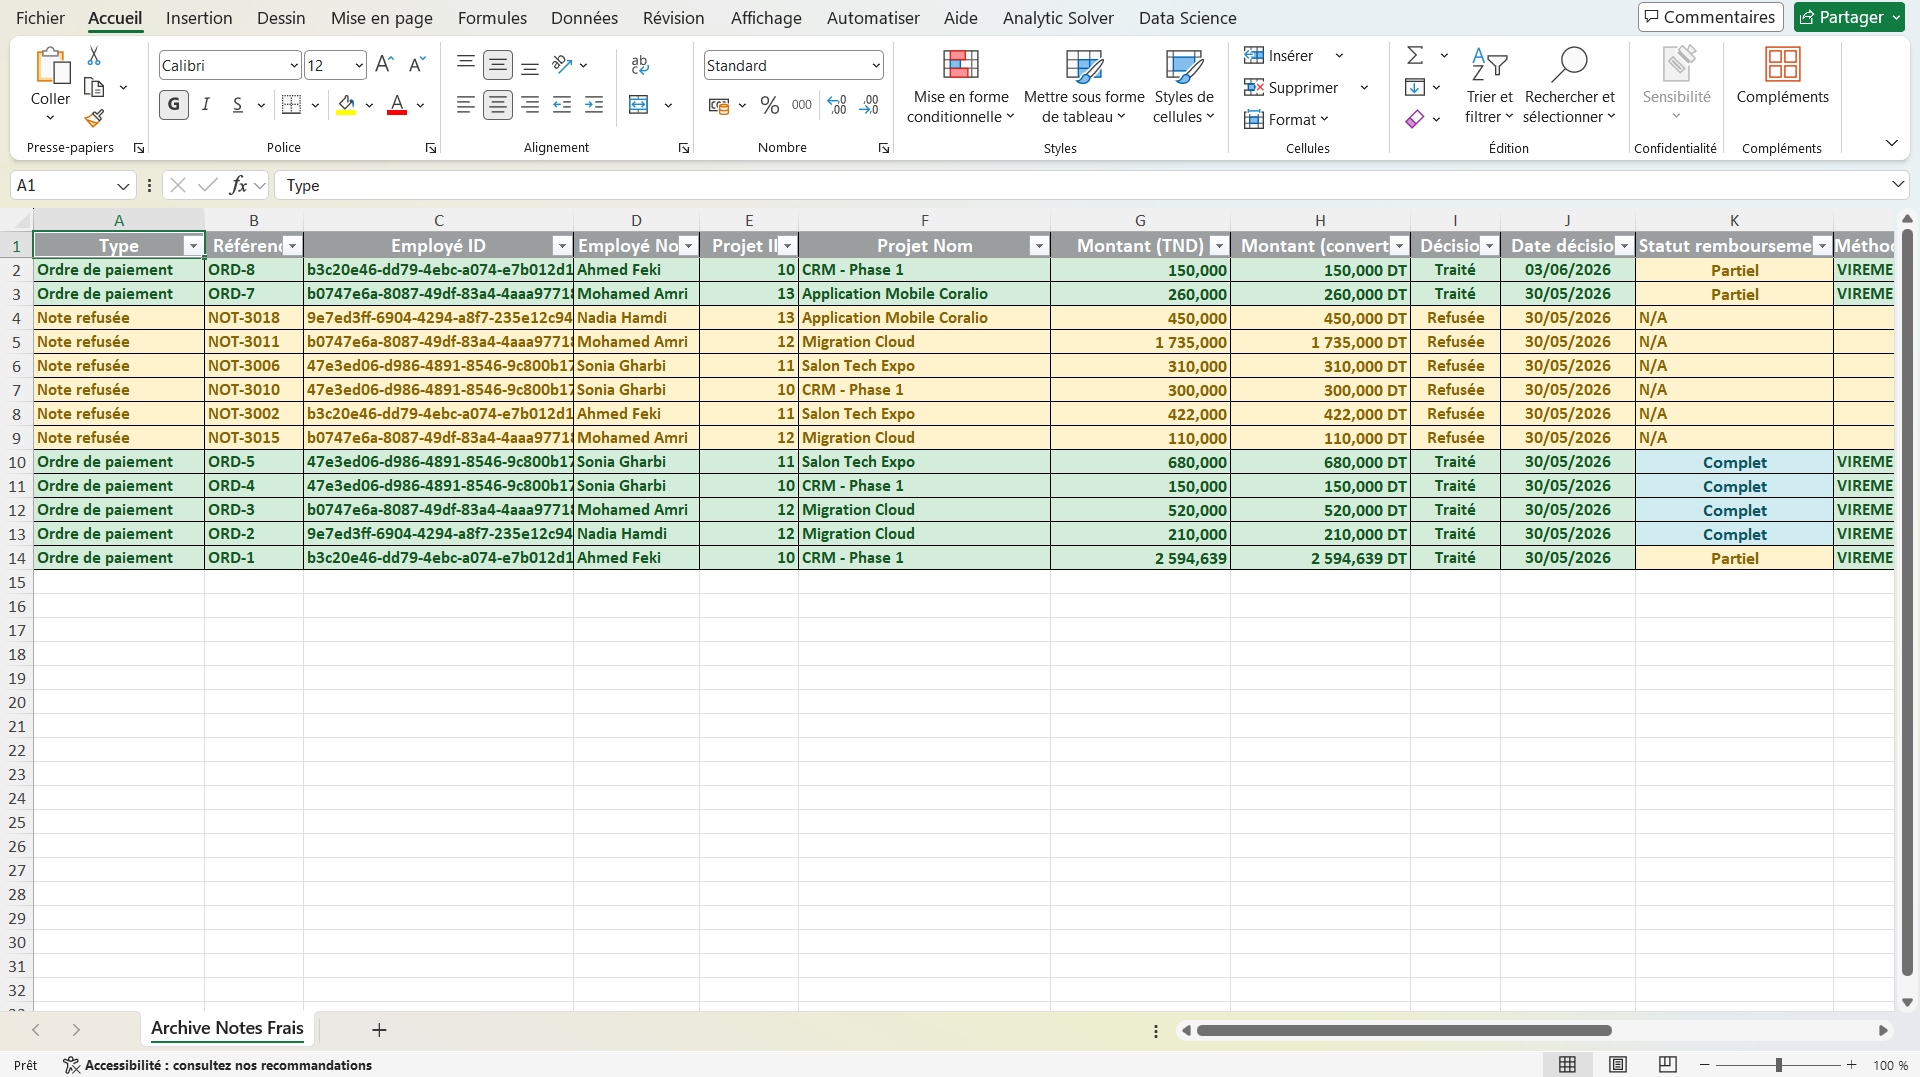
\includegraphics[width=\textwidth]{exported_data.png}

 \caption{Exemple de données exportées au format Excel}

 \label{fig:exported_data}

\end{figure}





\section{Déploiement avec Docker}



Pour simplifier le déploiement de l'application Coral.io Expense, nous avons conteneurisé chaque microservice ainsi que la base de données PostgreSQL et le serveur Keycloak. L'orchestration de l'ensemble est assurée par Docker Compose, permettant de lancer tous les services avec une seule commande.



\subsection{Avantages}

\begin{itemize}

 \item Environnement d'exécution identique en développement, test et production.

 \item Isolation des services (chacun dans son propre conteneur).

 \item Déploiement simplifié : \texttt{docker-compose up -d}.

 \item Facilité de montée en charge et de maintenance.

\end{itemize}



\subsection{Captures d'écran}



\begin{figure}[H]

 \centering

 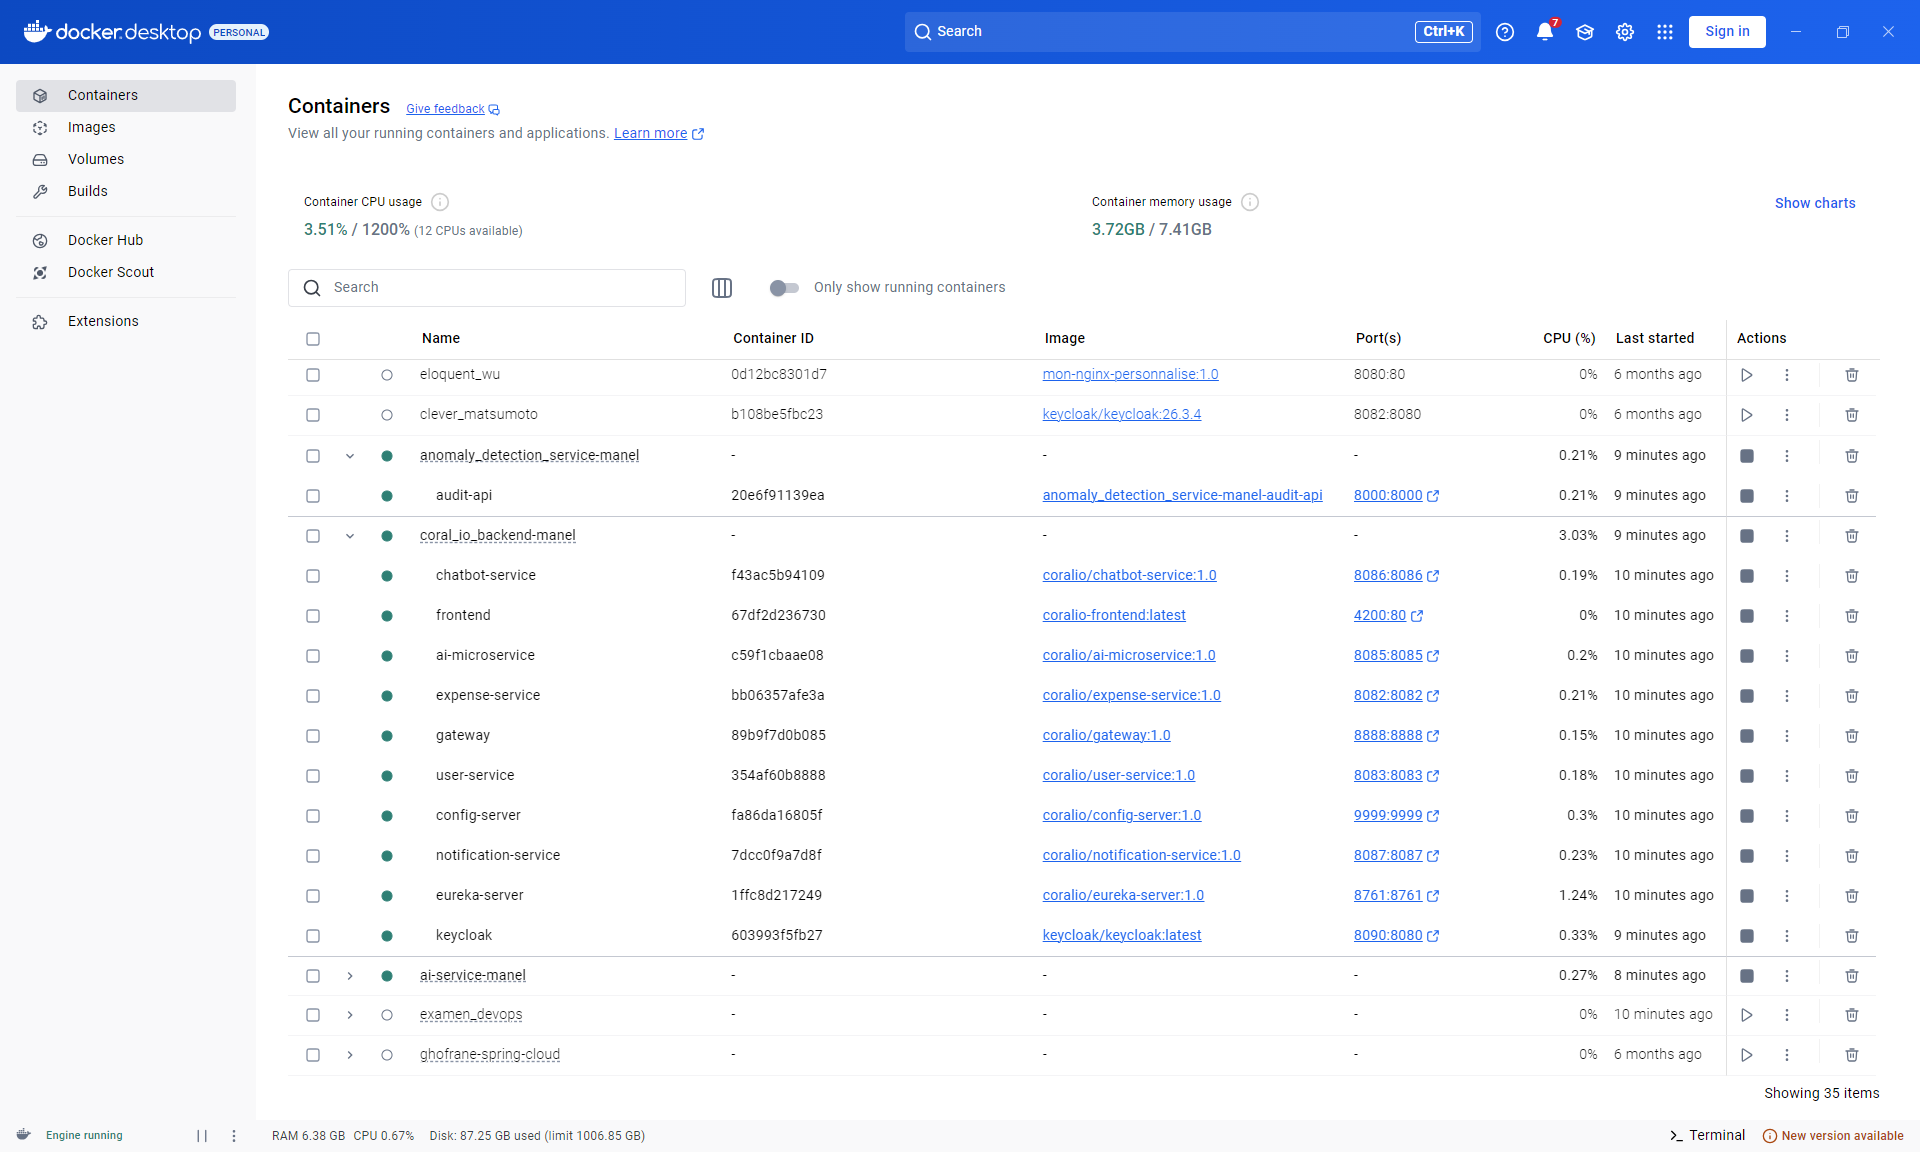
\includegraphics[width=0.9\textwidth,keepaspectratio]{docker_interface.png}

 \caption{Conteneurs Docker en cours d'exécution}

 \label{fig:docker_containers}

\end{figure}



\section*{Conclusion}

\addcontentsline{toc}{section}{Conclusion}

Le troisième sprint a livré l'intégralité du workflow de remboursement : l'administrateur peut consulter les notes validées, rembourser partiellement ou totalement, générer des ordres de paiement PDF, suivre les ordres en attente, confirmer les paiements, et consulter une archive complète de toutes les décisions finalisées. Les notifications associées assurent la transparence envers les employés. Ce sprint clôt le cycle de vie des notes de frais et prépare l'intégration des fonctionnalités avancées d'intelligence artificielle au sprint suivant.











\chapter{Sprint 4 – Détection des anomalies et Dashboards}



\section*{Introduction}

\addcontentsline{toc}{section}{Introduction}

Ce chapitre présente les travaux du Sprint 4, consacré à l'intégration de l'intelligence artificielle pour la détection automatique des anomalies ainsi qu'à la réalisation de tableaux de bord complets pour chaque utilisateur. Nous détaillons également l'assistant conversationnel (chatbot) hybride.



Contrairement aux sprints précédents, ce sprint requiert une approche orientée données et modèles. Nous avons donc orchestré son déroulement selon la méthodologie CRISP‑DM.



\section{Objectif du sprint}

L'objectif de ce sprint est de doter la plateforme Coral.io Expense de capacités d'analyse intelligente afin de réduire les risques de fraude et d'erreur, et de fournir des indicateurs de performance synthétiques et interactifs aux différents acteurs. Cela comprend la détection des doublons de justificatifs, l'analyse des montants suspects, le remplissage automatique des champs du formulaire à partir de la facture téléchargée, la comparaison sémantique entre un accord de mission et une note de frais, ainsi que la mise en place de dashboards personnalisés et d'un chatbot d'aide.



\section{Backlog du sprint 4}

Le tableau ci-dessous illustre la décomposition du sprint 4. La durée totale du sprint 4 est de 20 jours ouvrables (du 28/04 au 30/05).

\captionof{table}{Sprint 4 – User stories et tâches techniques associées}

\label{tab:sprint4_combined}

\begin{longtable}{|c|p{5cm}|p{5.5cm}|c|}

\hline

\textbf{ID} & \textbf{User Story} & \textbf{Tâches techniques} & \textbf{Durée (jours)} \\

\hline

\endfirsthead

\hline

\textbf{ID} & \textbf{User Story} & \textbf{Tâches techniques} & \textbf{Durée (jours)} \\

\hline

\endhead

\hline

\multicolumn{4}{|c|}{\textit{Suite dans la page suivante}} \\

\hline

\endfoot

\hline

\endlastfoot

US-64 & En tant qu'administrateur et manager, je veux que le système détecte automatiquement les doublons de justificatifs (factures et accords) lors de l'upload afin d'éviter les soumissions frauduleuses ou en erreur. & 

\begin{tabular}[t]{@{}p{5.5cm}@{}}

- Intégration du microservice Python (OCR, FAISS, SentenceTransformer) \\

- Endpoint Java : /check-duplicate \\

- Indexation des fichiers dans FAISS \\

- Affichage des doublons dans le popup de détail \\

- Tests

\end{tabular} & 2j \\

\hline

US-65 & En tant qu'administrateur et manager, je veux que le système analyse les montants des dépenses par catégorie et par utilisateur afin de détecter les montants anormalement élevés et de signaler les anomalies potentielles. & 

\begin{tabular}[t]{@{}p{5.5cm}@{}}

- Endpoint Java : /detect-anomaly-ai \\

- Service Python : Isolation Forest sur historique utilisateur/catégorie \\

- Ajout des champs \texttt{isAnomalyDepense}, \texttt{anomalyExpenseMessage} \\

- Affichage dans le popup de détail \\

- Tests

\end{tabular} & 1.5j \\

\hline

US-66 & En tant qu'administrateur et manager, je veux que le système analyse les factures afin de détecter les anomalies ou falsifications sur les justificatifs. & 

\begin{tabular}[t]{@{}p{5.5cm}@{}}

- Service Python d'extraction OCR (PaddleOCR) \\

- Endpoint /validate-receipt \\

- Comparaison des champs extraits avec les données saisies (montant, date, commerçant) \\

- Stockage du résultat d'analyse \\

- Affichage dans le popup de détail \\

- Tests

\end{tabular} & 2j \\

\hline

US-67 & En tant qu'administrateur et manager, je veux que le système compare automatiquement les données du formulaire de note de frais avec l'accord de mission associé (dates, lieu, objectif, etc.) afin de détecter les anomalies sémantiques et contextuelles. & 

\begin{tabular}[t]{@{}p{5.5cm}@{}}

- Endpoint /analyze-full (Java appellera le microservice Python) \\

- Service Python : extraction structurée de l'accord + LLM (Gemma3:4b) \\

- Comparaison avec formulaire Angular (règles métier + LLM) \\

- Stockage du résultat JSON dans \texttt{aiAnalysisResult} \\

- Affichage via onglets (anomalies, extrait, conclusion) dans le popup \\

- Tests

\end{tabular} & 3j \\

\hline

US-68 & En tant qu'employé, je veux que le système remplisse automatiquement les champs du formulaire (montant, date, description, etc.) à partir de la facture téléchargée, afin de gagner du temps et de réduire les erreurs de saisie. & 

\begin{tabular}[t]{@{}p{5.5cm}@{}}

- Backend: endpoint /extract-fields appelant le microservice IA \\

- Frontend: affichage des champs extraits et application automatique \\

- Tests

\end{tabular} & 2j \\

\hline

US-69 & En tant qu'employé, je veux visualiser des statistiques personnalisées sur mes propres notes afin de suivre l'évolution de mes dépenses. & 

\begin{tabular}[t]{@{}p{5.5cm}@{}}

- Création du composant \texttt{EmployeeDashboard} \\

- Graphiques : évolution du nombre de notes, évolution des montants, répartition par catégorie et statut \\

- Alertes personnelles (dépassement de plafond, notes bloquées) \\

- Intégration du filtre période (aujourd'hui, semaine, mois, personnalisé) \\

- Tests

\end{tabular} & 2j \\

\hline

US-70 & En tant que manager, je veux disposer d'un tableau de bord complet avec des statistiques synthétiques sur les dépenses de mon département, l'état d'avancement des notes et les alertes budgétaires. & 

\begin{tabular}[t]{@{}p{5.5cm}@{}}

- Composant \texttt{ManagerDashboard} \\

- KPIs : notes en attente, montant total en attente, délai moyen traitement \\

- Graphiques : évolution des soumissions, top dépensiers, répartition par statut, dépenses par catégorie, consommation budget par projet \\

- Liste des anomalies IA et doublons par note \\

- Tests

\end{tabular} & 2j \\

\hline

US-71 & En tant qu'administrateur, je veux consulter un tableau de bord global avec des indicateurs clés (nombre total de notes, montants remboursés par mois, anomalies détectées, délais de traitement) afin de piloter la performance financière. & 

\begin{tabular}[t]{@{}p{5.5cm}@{}}

- Composant \texttt{AdminDashboard} \\

- KPIs : notes en attente de validation admin, montant remboursé, ordres à payer, taux validation admin \\

- Graphiques : évolution financière, top dépensiers, catégories, fraudes par type, performance managers, budget consommé par projet, calendrier des remboursements \\

- Export Excel/CSV des données \\

- Tests

\end{tabular} & 2j \\

\hline

US-72 & En tant qu'utilisateur, je veux poser des questions au chatbot hybride afin d'obtenir une aide instantanée sur les règles de remboursement ou l'état de mes notes. & 

\begin{tabular}[t]{@{}p{5.5cm}@{}}

- Composant Angular \texttt{Chatbot} \\

- Backend : endpoint de dialogue avec LLM local (Ollama) \\

- Intégration dans les pages employé, manager, admin \\

- Tests

\end{tabular} & 3.5j \\

\hline

\multicolumn{3}{|c|}{\textbf{Total}} & \textbf{19.5j} \\

\hline

\end{longtable}





\section{Analyse}



\subsection{Diagramme des cas d'utilisation}

Le diagramme des cas d'utilisation ci-dessous illustre les interactions entre les acteurs (Employé, Manager, Administrateur) et les fonctionnalités introduites lors du sprint 4.



\begin{figure}[H]

 \centering

 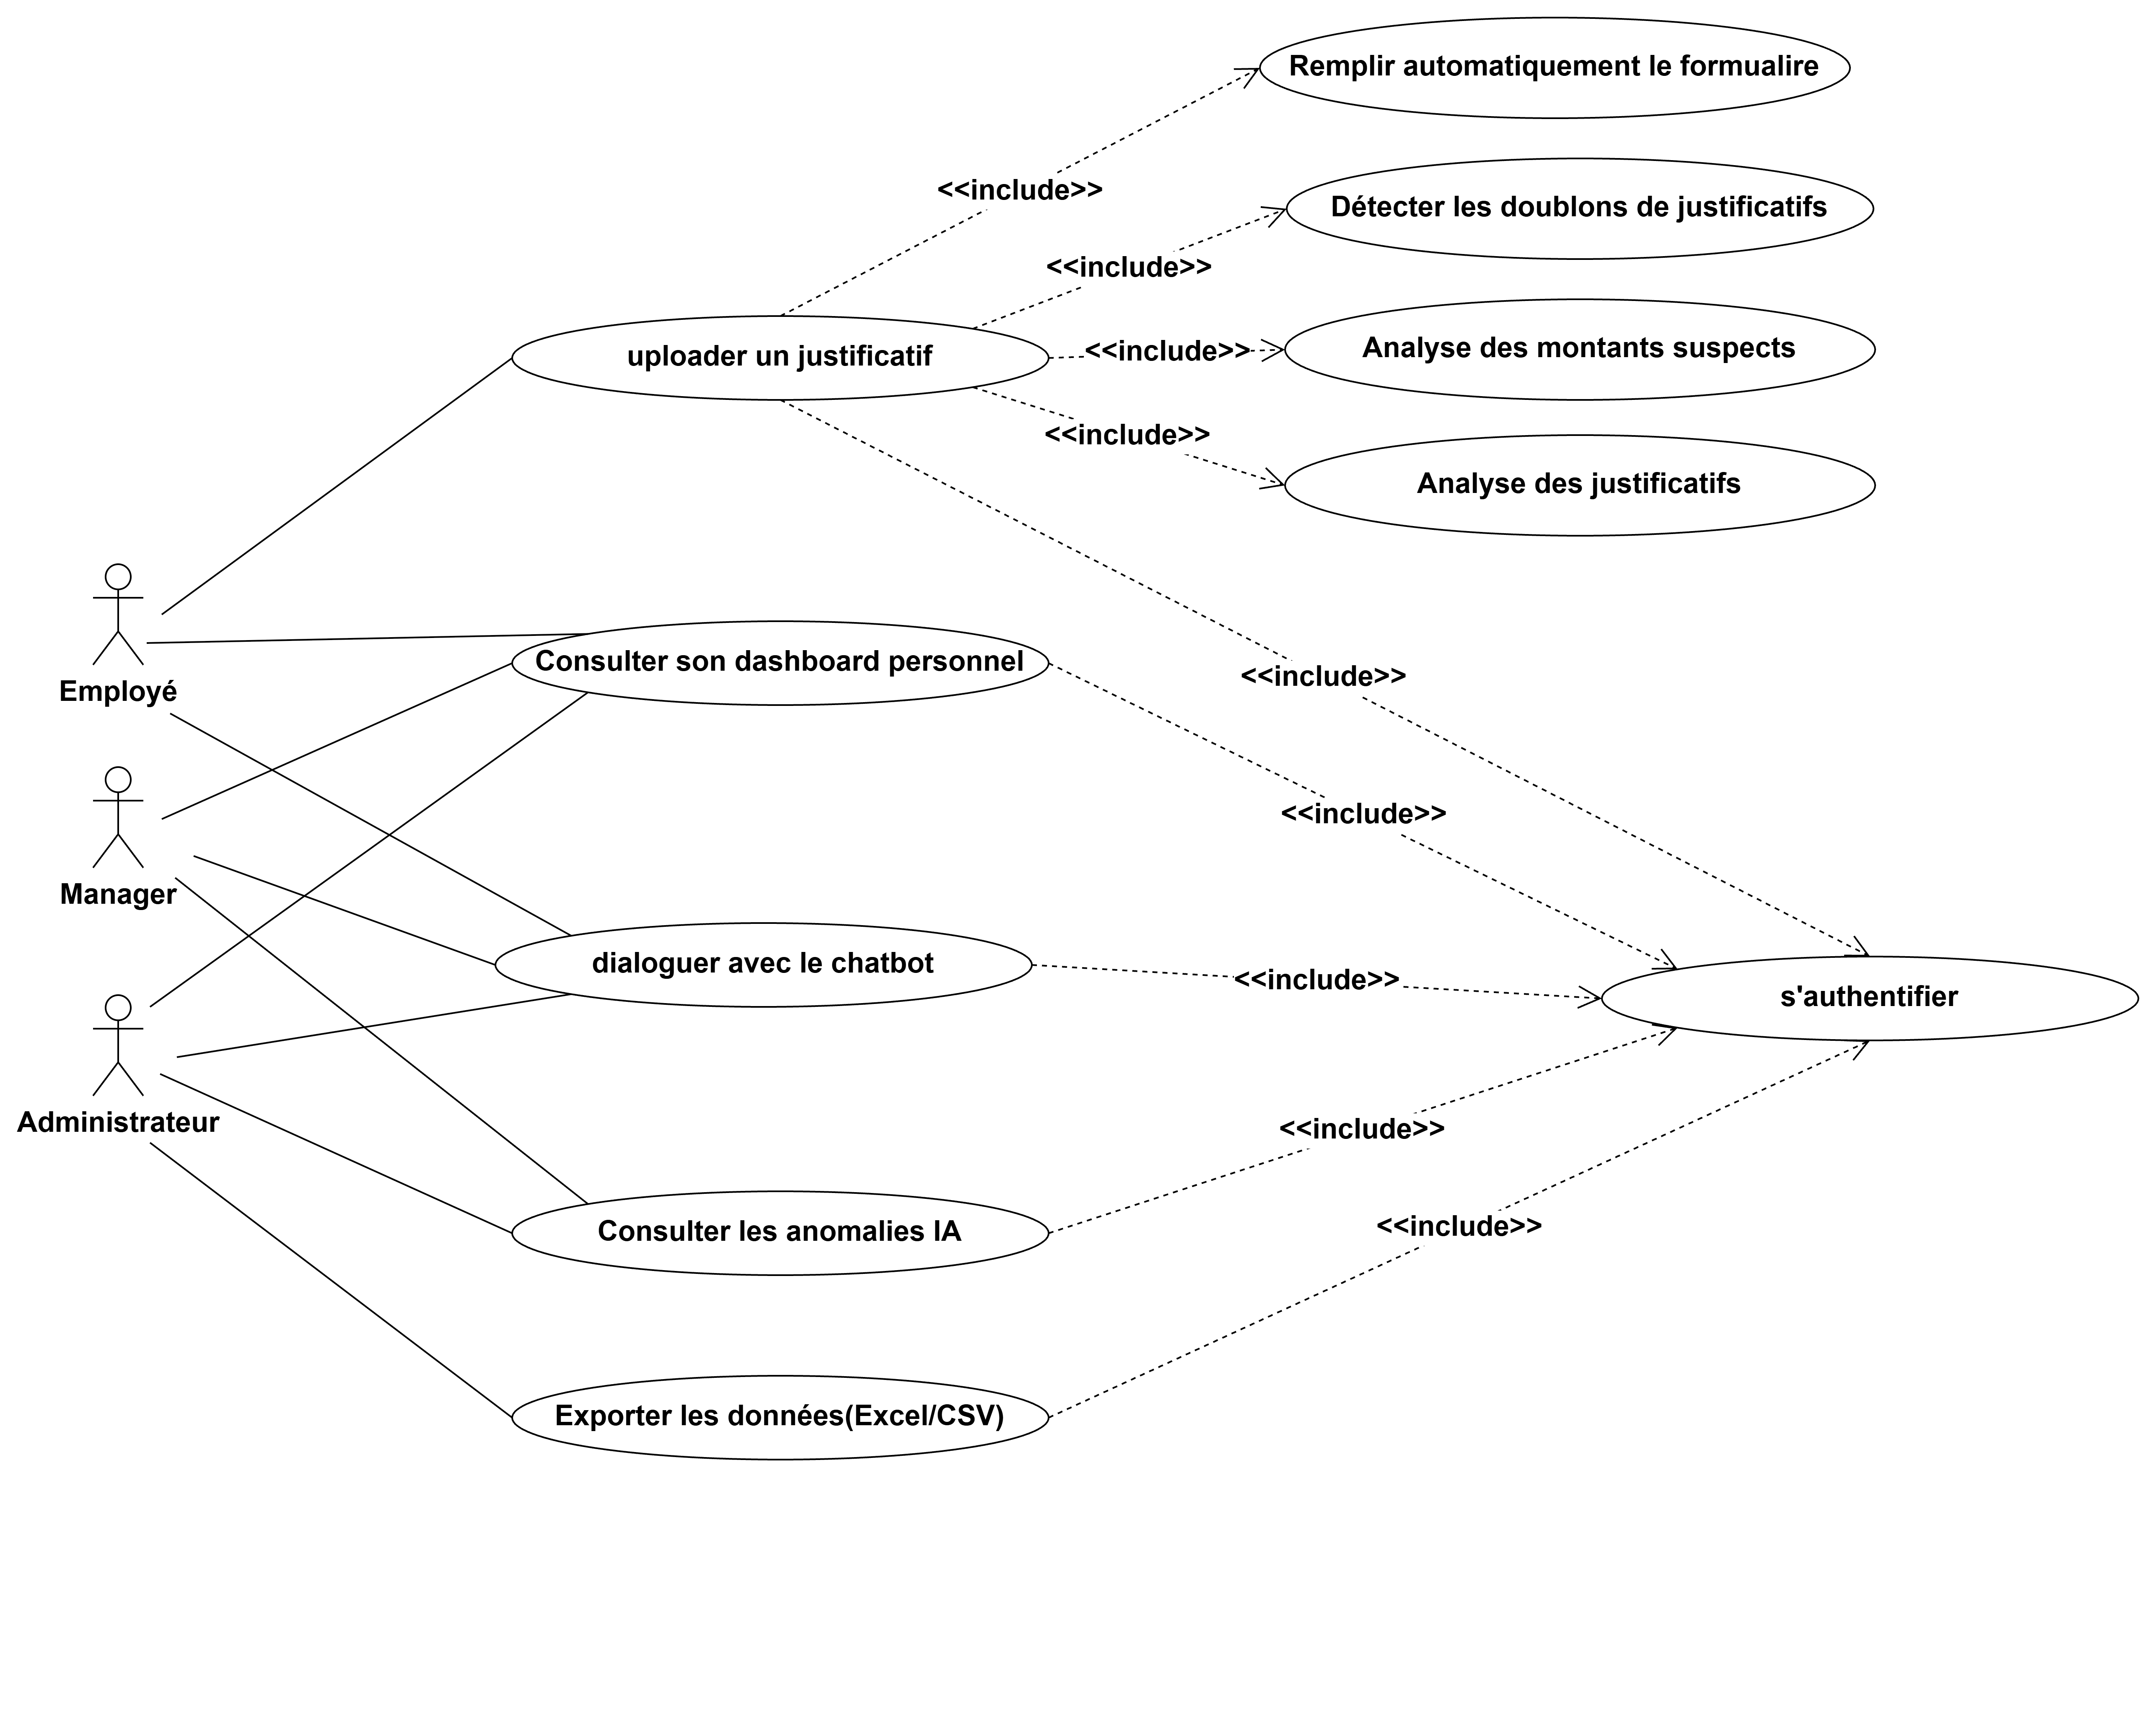
\includegraphics[width=\textwidth,height=0.6\textheight]{usecase_sprint4.png}

 \caption{Diagramme des cas d'utilisation du sprint 4}

 \label{fig:usecase_sprint4}

\end{figure}



\subsection{Description textuelle des cas d'utilisation}



\subsection*{Description textuelle -- Téléverser un justificatif et déclencher les analyses automatiques}

\captionof{table}{Description textuelle – Téléverser un justificatif et déclencher les analyses automatiques}

\label{tab:upload_justificatif_desc}

\begin{longtable}{|p{3cm}|p{11cm}|}

\hline

Élément & Description \\

\hline

\endfirsthead

\hline

Élément & Description \\

\hline

\endhead

\hline

\multicolumn{2}{|c|}{\textit{Suite dans la page suivante}} \\

\hline

\endfoot

\hline

\endlastfoot

Titre & Téléverser un justificatif et déclencher les analyses automatiques \\

\hline

Acteur & Employé \\

\hline

But & Déposer un justificatif (facture ou accord) lors de la création d'une note de frais et déclencher l'ensemble des contrôles automatiques (doublons, OCR, remplissage, montants suspects, comparaison avec accord de mission) \\

\hline

Précondition & L'employé est authentifié et est en train de créer/modifier une note de frais \\

\hline

\multirow{12}{*}{Scénario nominal} & 1. L'employé clique sur "Téléverser un justificatif" \\

& 2. Le système affiche une fenêtre de sélection de fichier \\

& 3. L'employé sélectionne un fichier (PDF, JPEG, PNG, DOCX) \\

& 4. Le système vérifie le format et la taille (< 10 Mo) \\

& 5. Le système détecte automatiquement les doublons via l'index FAISS (similarité > 0,95) \\

& 6. Le système extrait le texte du justificatif (OCR via PaddleOCR si nécessaire) \\

& 7. Si le justificatif est une facture, le système pré-remplit automatiquement les champs (montant, date, description, commerçant) \\

& 8. Le système analyse le montant saisi via Isolation Forest (comparaison avec l'historique employé/catégorie) \\

& 9. Si un accord de mission est associé à la note, le système compare sémantiquement les données (dates, lieu, objectif) via LLM (Gemma3:4b) \\

& 10. Le système affiche un aperçu du justificatif téléversé \\

& 11. L'employé peut ajouter plusieurs justificatifs \\

& 12. Un message de confirmation s'affiche \\

\hline

\multirow{6}{*}{Scénario alternatif} & 4.1 Format invalide : le système affiche "Format non supporté" \\

& 4.2 Taille > 10 Mo : le système affiche "Fichier trop volumineux" \\

& 5.1 Doublon détecté : le système alerte l'employé et bloque la soumission \\

& 7.1 Échec de l'OCR : le système affiche "Extraction automatique impossible, veuillez saisir manuellement" \\

& 8.1 Historique insuffisant : le système utilise uniquement les plafonds de catégorie \\

& 9.1 Échec d'extraction de l'accord : aucun résultat de comparaison n'est stocké \\

\hline

Post-condition & Le justificatif est stocké sur le serveur, associé à la note de frais, et l'ensemble des résultats d'analyse (doublons, anomalies de montant, comparaison accord) est enregistré dans la base de données \\

\hline

\end{longtable}



\subsection*{Description textuelle -- Consulter les anomalies IA}

\captionof{table}{Description textuelle – Consulter les anomalies IA}

\label{tab:gerer_anomalies_desc}

\begin{longtable}{|p{3cm}|p{11cm}|}

\hline

Élément & Description \\

\hline

\endfirsthead

\hline

Élément & Description \\

\hline

\endhead

\hline

\multicolumn{2}{|c|}{\textit{Suite dans la page suivante}} \\

\hline

\endfoot

\hline

\endlastfoot

Titre & Consulter les anomalies IA \\

\hline

Acteur & Manager / Administrateur \\

\hline

But & Visualiser les anomalies détectées automatiquement par l'IA sur les notes de frais\\

\hline

Précondition & L'utilisateur est authentifié avec le rôle Manager ou Administrateur \\

\hline

\multirow{8}{*}{Scénario nominal} & 1. L'utilisateur accède à son tableau de bord (ManagerDashboard ou AdminDashboard) \\

& 2. Le système affiche la section "Alertes et anomalies" avec les KPIs pertinents \\

& 3. L'utilisateur voit la liste des notes comportant des anomalies détectées par l'IA \\

& 4. Il clique sur une note pour ouvrir le popup de détail \\

& 5. Le système affiche les anomalies dans l'onglet dédié : \\

& \hspace{0.5cm} - Doublons de justificatifs \\

& \hspace{0.5cm} - Montants suspects (avec message d'anomalie) \\

& \hspace{0.5cm} - Résultat de comparaison avec l'accord de mission (anomalies listées, extraits, conclusion) \\

& \hspace{0.5cm} - Résultat d'analyse OCR/LLM de la facture \\

& 6. L'utilisateur peut consulter les détails de chaque anomalie \\

& 7. Selon l'anomalie, il peut : valider la note, la refuser, ou demander des justificatifs complémentaires \\

\hline

Scénario alternatif & Aucune anomalie : la section affiche "Aucune anomalie à signaler" \\

\hline

Post-condition & L'utilisateur a pris une décision sur les notes anormales ; la note de frais avance dans son workflow de validation avec le statut approprié \\



\end{longtable}



\section{Système de Détection des anomalies}



\subsection{Architecture globale des détections IA}

Afin d'automatiser les contrôles de conformité et de détecter les fraudes potentielles, nous avons mis en place une architecture distribuée reposant sur plusieurs microservices :

\begin{itemize}

 \item \textbf{Microservice Java (port 8888)} : orchestration des appels aux services IA.

 \item \textbf{Microservice Python d'analyse de documents (port 8000)} : extraction des données structurées à partir des accords de mission (PDF, images, DOCX) et comparaison avec le formulaire.

 \item \textbf{Microservice Python unifié (port 9000)} : détection de doublons (FAISS), analyse des factures (OCR + LLM), détection des montants suspects (Isolation Forest), et extraction automatique des champs.

 \item \textbf{Ollama (port 11434)} : serveur local de LLM (Gemma3:4b et Mistral:7b) pour les analyses sémantiques.

\end{itemize}



\subsection{Cycle de vie d'une note de frais avec les contrôles automatiques}

Le schéma ci-dessous illustre l'enchaînement des vérifications effectuées lors de la soumission d'une note de frais.



\begin{figure}[H]

 \centering

 \includegraphics[width=0.9\textwidth,keepaspectratio]{cycle_modif.png}

 \caption{Cycle de vie de soumission d'une note de frais avec les contrôles automatiques}

 \label{fig:lifecycle}

\end{figure}



\subsection{Diagramme de classes}

Le diagramme de classes ci-dessous présente les principales entités et leurs attributs/méthodes introduites ou enrichies lors de ce sprint.



\begin{figure}[H]

\centering

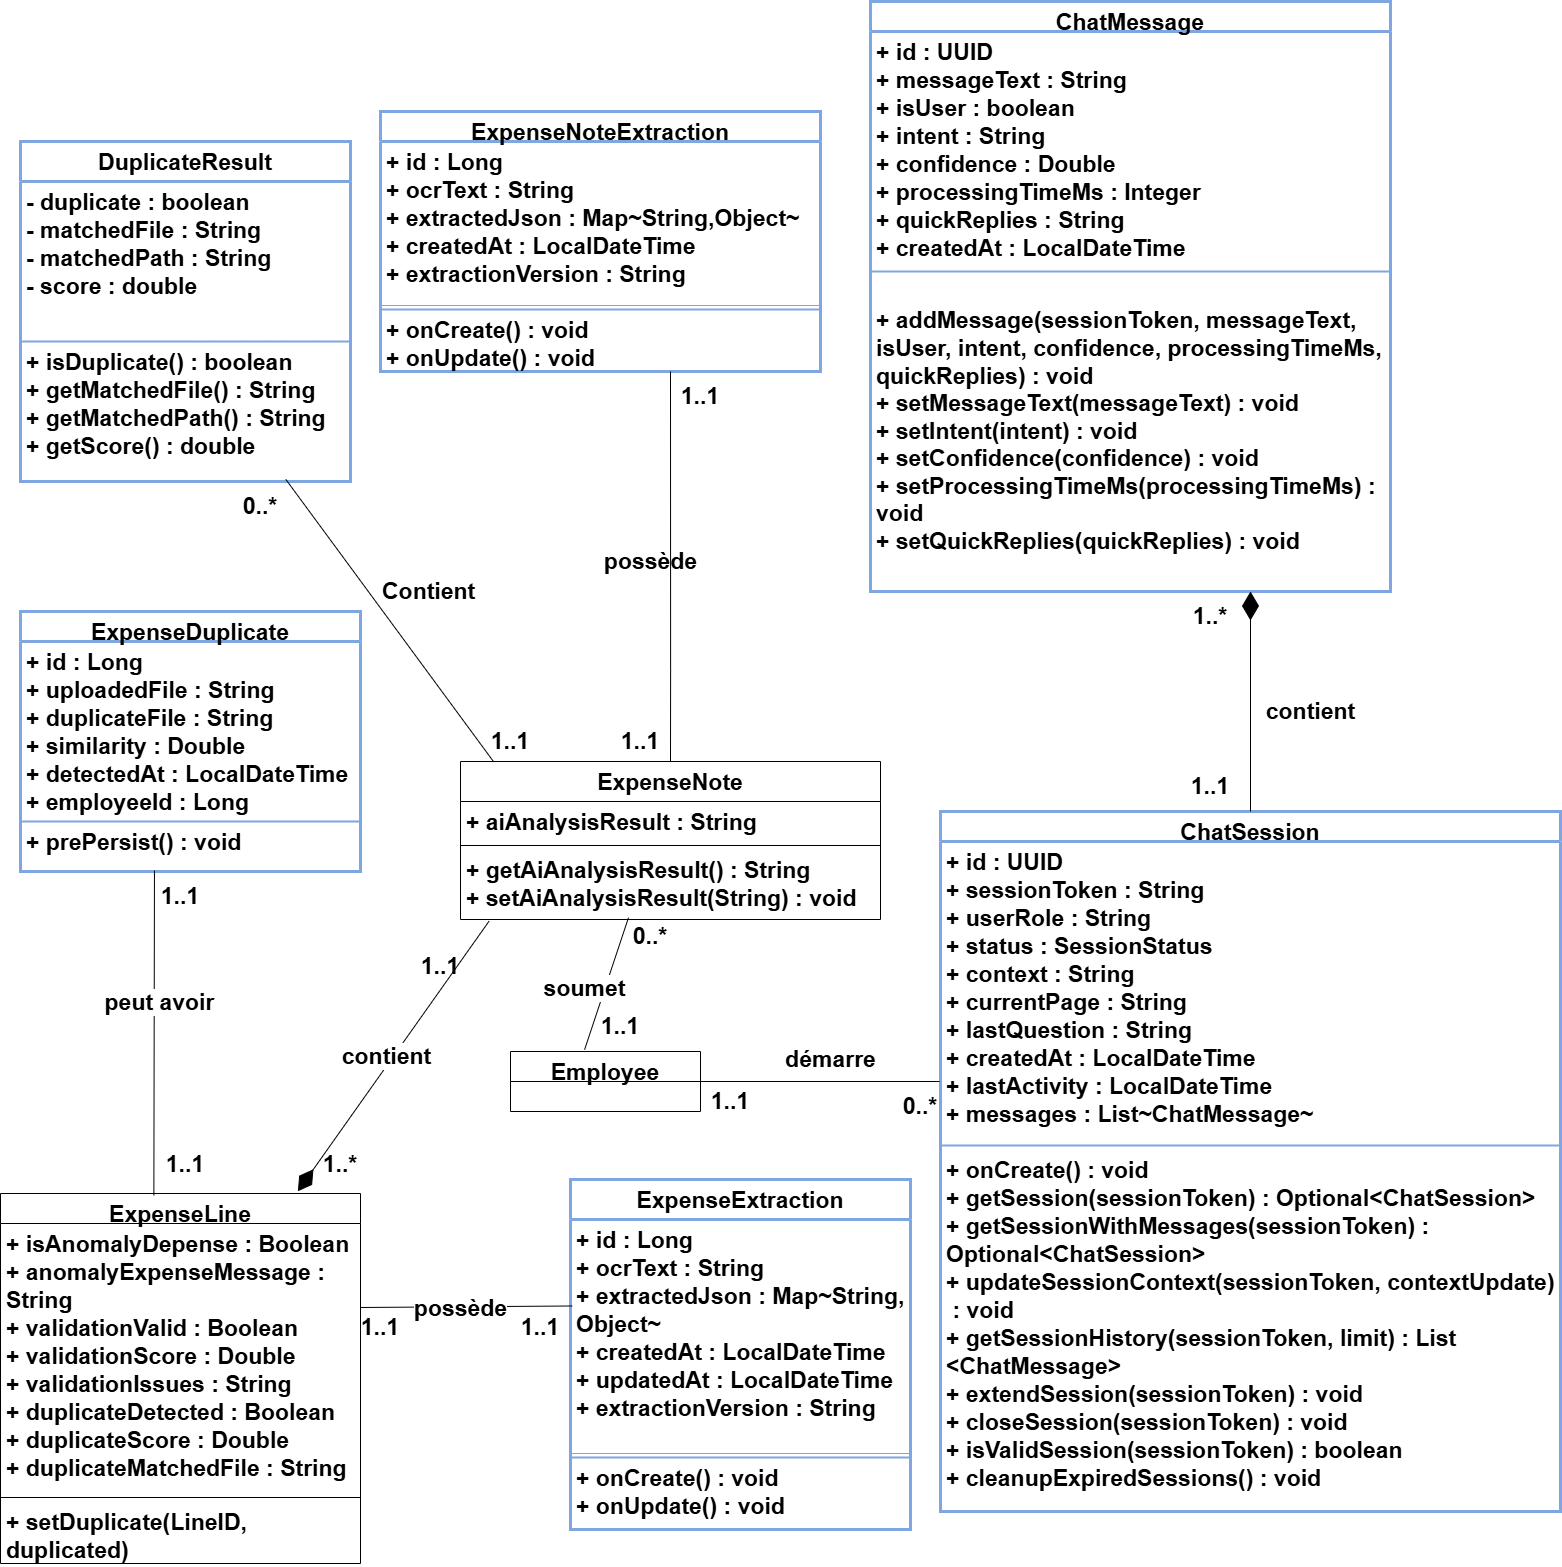
\includegraphics[width=0.9\textwidth,height=0.75\textheight]{class_diagram_sprint4.png}

\caption{Diagramme de classes du sprint 4 (extrait)}

\label{fig:class_sprint4}

\end{figure}



\subsection{Diagramme de déploiement}

Le diagramme de déploiement ci-dessous présente l'architecture physique des composants déployés lors du sprint 4.



\begin{figure}[H]

\centering

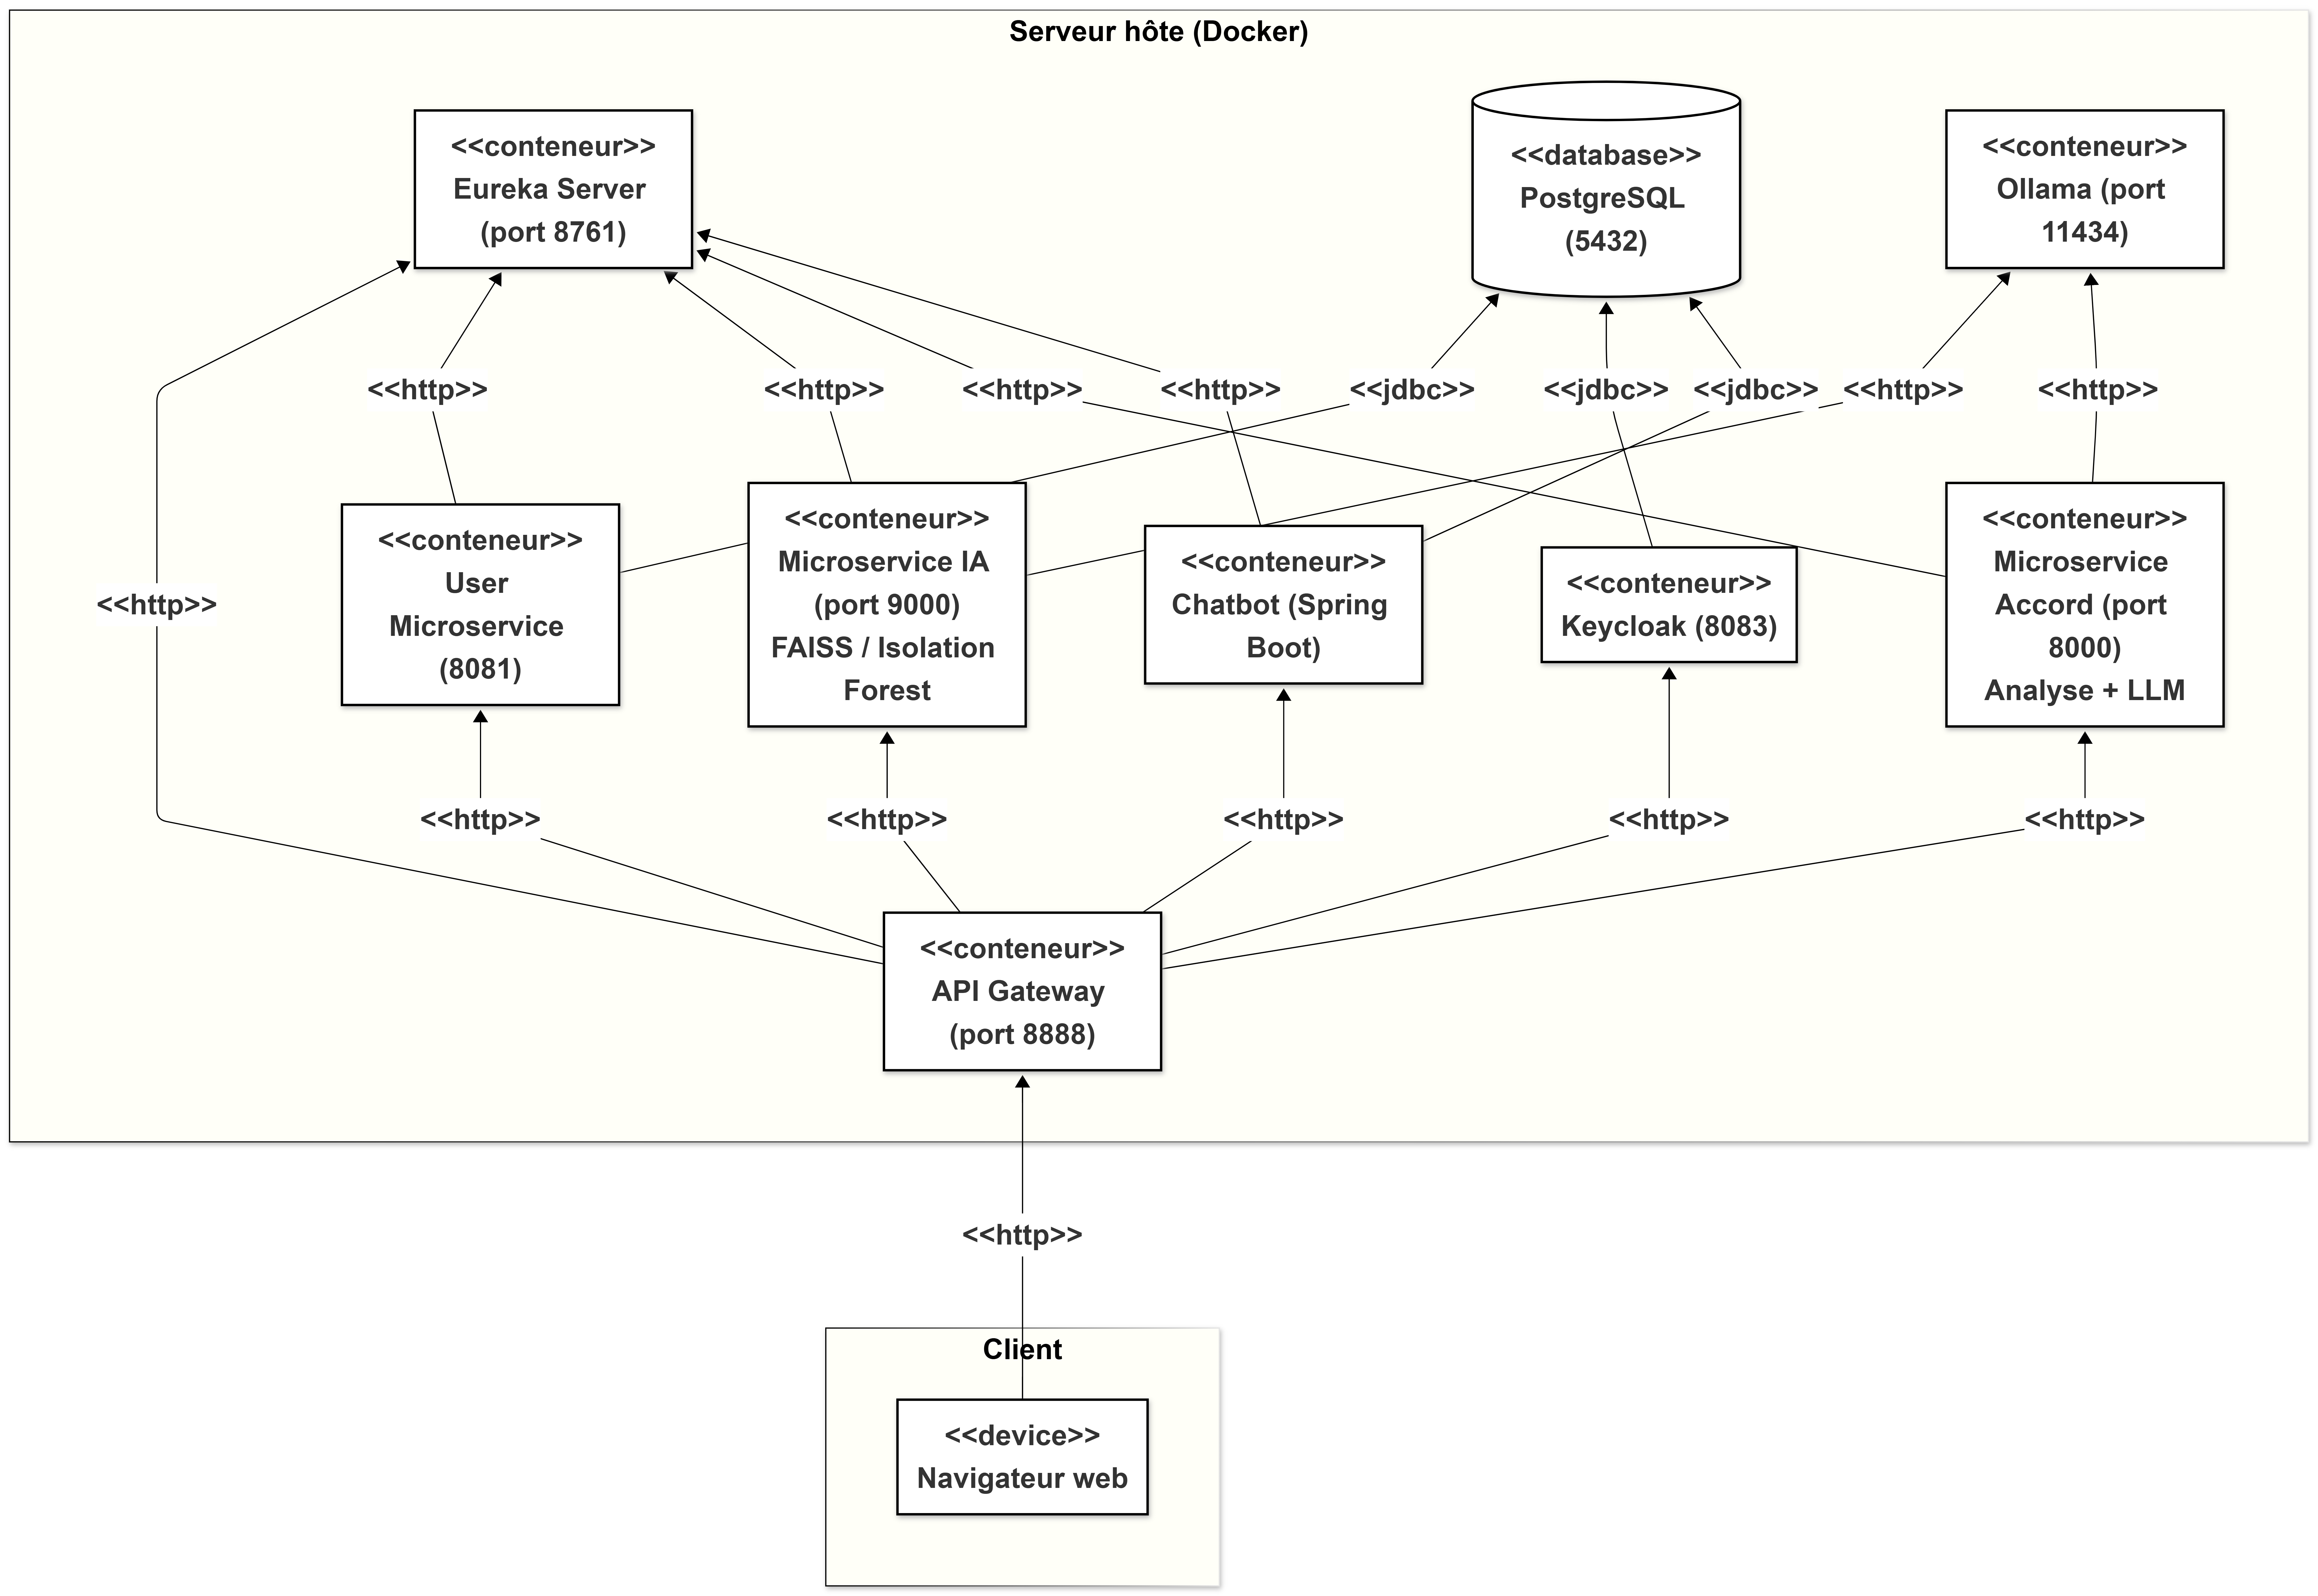
\includegraphics[width=1.2\textwidth,height=0.88\textwidth,angle=90,keepaspectratio]{deploiement_sp4.png}

\caption{Diagramme de déploiement du sprint 4}

\label{fig:deploiement_sprint4}

\end{figure}

\subsection{Pourquoi CRISP-DM ?}

La détection des anomalies dans les notes de frais ne se limite pas à l’implémentation d’un modèle : elle nécessite une approche structurée couvrant l’ensemble du cycle de vie des données. CRISP-DM a été retenu car :

\begin{itemize}

 \item Il est indépendant de tout outil ou technologie, ce qui permet de l’adapter à notre architecture microservices.

 \item Ses phases itératives (compréhension du métier, des données, préparation, modélisation, évaluation, déploiement) correspondent parfaitement au besoin d’amélioration continue des modèles.

 \item Il favorise une collaboration étroite entre experts métier (administrateurs, managers) et data scientists, essentielle pour définir ce qu’est une « anomalie ».

 \item Il intègre une phase d’évaluation rigoureuse (matrice de confusion, métriques de précision/rappel) avant le déploiement, limitant ainsi les risques de faux positifs en production.

\end{itemize}

Ainsi, l’application de CRISP-DM garantit que chaque fonctionnalité IA est développée de manière méthodique, traçable et alignée sur les objectifs métier du sprint 4.





\subsection{Compréhension du métier}

L'objectif principal est de réduire les risques de fraude et d'erreur dans le processus de remboursement des notes de frais. Concrètement, il s'agit de :

\begin{itemize}

 \item Détecter automatiquement les doublons de justificatifs (factures, accords) pour empêcher une soumission frauduleuse.

 \item Identifier les montants anormalement élevés par rapport à l'historique de l'employé dans une catégorie donnée.

 \item Analyser les factures (OCR + LLM) pour vérifier si le justificatif est valide ou non.

 \item Comparer l'accord de mission signé avec les données du formulaire de note de frais pour détecter des incohérences sémantiques ou contextuelles (dates, lieu, objectif, identité, projet).

\end{itemize}

Ces fonctionnalités constituent un système d'aide à la décision mis à disposition des administrateurs et des managers, leur permettant de statuer sur les notes de frais avec davantage de fiabilité et de traçabilité.

\subsection{Compréhension des données}

La compréhension des données constitue une étape fondamentale dans la démarche CRISP-DM. Elle permet d'identifier les sources disponibles, d'évaluer leur qualité et de mieux cerner les caractéristiques des données sur lesquelles reposera la détection des anomalies.



% Inclure les subsubsection dans la numérotation et la TOC

\setcounter{secnumdepth}{3}

\setcounter{tocdepth}{3}



% Format de numérotation : a), b), c), ...

\renewcommand{\thesubsubsection}{\alph{subsubsection})}

\subsubsection{Collecte des données}

Avant toute modélisation, il est indispensable d'identifier et de centraliser l'ensemble des données nécessaires à l'analyse. Ces données proviennent de sources hétérogènes qu'il convient de collecter, extraire et structurer.



\textbf{a.1. Sources des données}\\

Les données mobilisées dans ce projet proviennent de trois sources complémentaires :

\begin{itemize}

 \item \textbf{Justificatifs (factures, accords)} : fichiers PDF, images (JPEG, PNG), documents Word (DOCX) déposés par les employés lors de la soumission de leurs notes de frais.

 \item \textbf{Base de données PostgreSQL} : historique des notes de frais, lignes de dépenses, catégories, projets, utilisateurs, ordres de paiement.

 \item \textbf{Données externes} : taux de change issus d'une API externe, et règles de validation métier (plafonds par catégorie, jours fériés tunisiens).

\end{itemize}



\textbf{a.2. Présentation et évaluation des outils OCR}\\

Avant de décrire le processus de collecte, nous présentons les outils retenus pour l'extraction du texte, ce choix conditionnant directement les étapes du pipeline.

Nous avons testé trois moteurs OCR : \textbf{PaddleOCR}, \textbf{Tesseract} et l’extraction directe par \textbf{pdfplumber} (pour les PDF textuels). Le tableau suivant résume leurs caractéristiques.



\begin{table}[H]

\centering

\caption{Comparaison des outils OCR utilisés}

\label{tab:ocr_comparison}

\begin{tabular}{|p{2.5cm}|p{3cm}|p{3cm}|p{3cm}|}

\hline

\textbf{Critère} & \textbf{PaddleOCR} & \textbf{Tesseract} & \textbf{pdfplumber} \\

\hline

Facilité d’usage & Moyenne (nécessite configuration) & Facile (installation simple) & Très facile (intégration Python) \\

\hline

Précision & Très bonne, gère multi-langues (français, anglais, arabe) & Bonne, mais moins fiable sur texte dégradé & Parfaite pour PDF textuels (extraction du texte natif sans OCR) \\

\hline

Types supportés & Images, PDF (via conversion) & Images, PDF (via conversion) & PDF textuels uniquement \\

\hline

Coût & Gratuit & Gratuit & Gratuit \\

\hline

Points faibles & Lourd en mémoire, nécessite GPU pour performance & Moins précis sur polices atypiques & Ne fonctionne pas sur PDF scannés \\

\hline

\end{tabular}

\end{table}



À l'issue de cette comparaison, nous avons retenu la stratégie suivante : \texttt{pdfplumber} est privilégié pour les accords de mission au format PDF textuel, \texttt{PaddleOCR} est utilisé pour les images et PDF scannés, et \texttt{Tesseract} intervient en solution de repli. Pour les factures, \texttt{PaddleOCR} offre les meilleurs résultats en termes de précision.



\textbf{a.3. Processus de collecte}\\

Fort de ces choix techniques, le pipeline de collecte suit les étapes suivantes :

\begin{itemize}

 \item \textbf{Upload des fichiers} : l’employé dépose un justificatif (facture) ou un accord.

 \item \textbf{Extraction par OCR} : selon le type de fichier, le système choisit l’outil le plus adapté : \texttt{pdfplumber} pour les PDF textuels, \texttt{PaddleOCR} pour les images et PDF scannés, et \texttt{Tesseract} en solution de repli.

 \item \textbf{Structuration par LLM} : le texte brut extrait est transmis au modèle Gemma3:4b (via Ollama) pour être structuré en JSON (montant, date, description, commerçant, etc.).

 \item \textbf{Vérification automatique} : les champs extraits sont comparés aux données saisies manuellement par l’employé afin de détecter d’éventuelles incohérences.

 \item \textbf{Stockage} : les résultats d’extraction et d’analyse sont conservés dans les tables \texttt{expense\_extractions}, \texttt{expense\_note\_extractions} ainsi que dans le champ \texttt{ai\_analysis\_result} de la note de frais.

\end{itemize}

\textbf{a.4. Exemples d’extraction par PaddleOCR et Tesseract}\\

Les figures ci-dessous montrent la détection des zones de textes depuis les fichiers via OCR :

\begin{itemize}

 \item \textbf{Extraction par PaddleOCR}

 \begin{itemize}[label=--] % nécessite le package enumitem

 \item Extraction par PaddleOCR depuis un PDF :

 \begin{figure}[H]

 \centering

 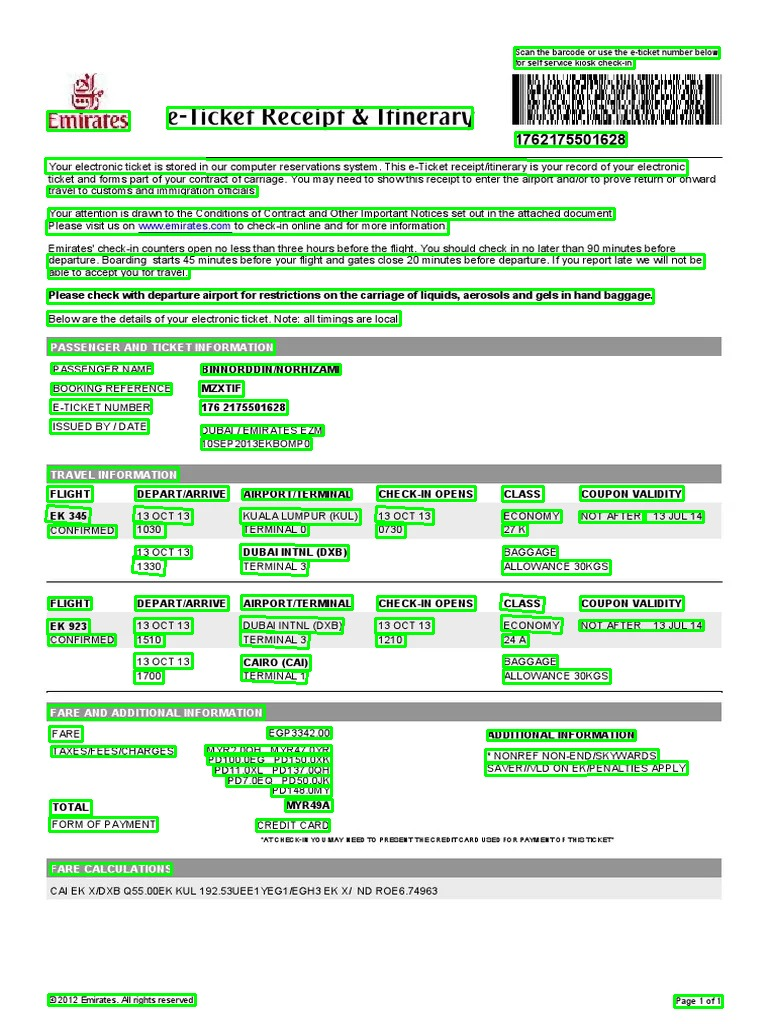
\includegraphics[width=0.7\textwidth]{paddle_ocr.png}

 \caption{Extraction par PaddleOCR pour un PDF}

 \label{fig:paddle_ocr}

 \end{figure}

 \item Extraction par PaddleOCR depuis une image PNG :

 \begin{figure}[H]

 \centering

 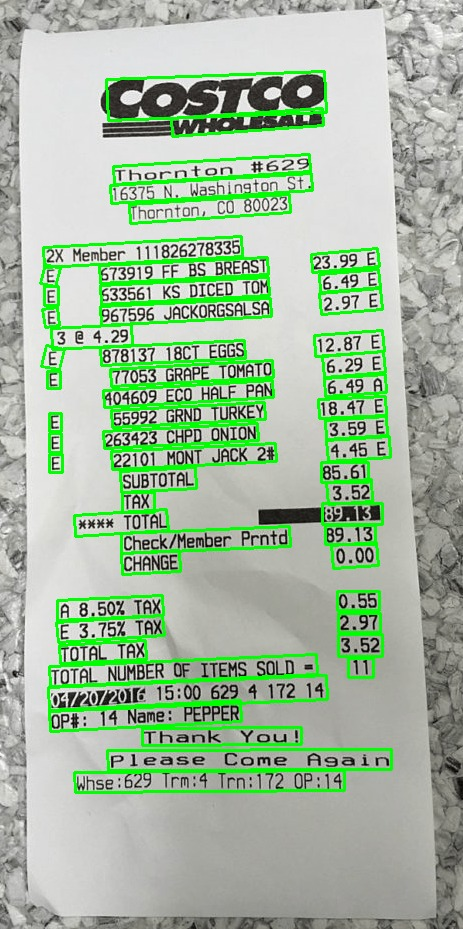
\includegraphics[width=0.7\textwidth,height=0.5\textheight]{paddle_ocr2.png}

 \caption{Extraction par PaddleOCR pour un PNG}

 \label{fig:paddle_ocr2}

 \end{figure}

 \end{itemize}

\newpage

 \item \textbf{Extraction par Tesseract}

 \begin{figure}[H]

 \centering

 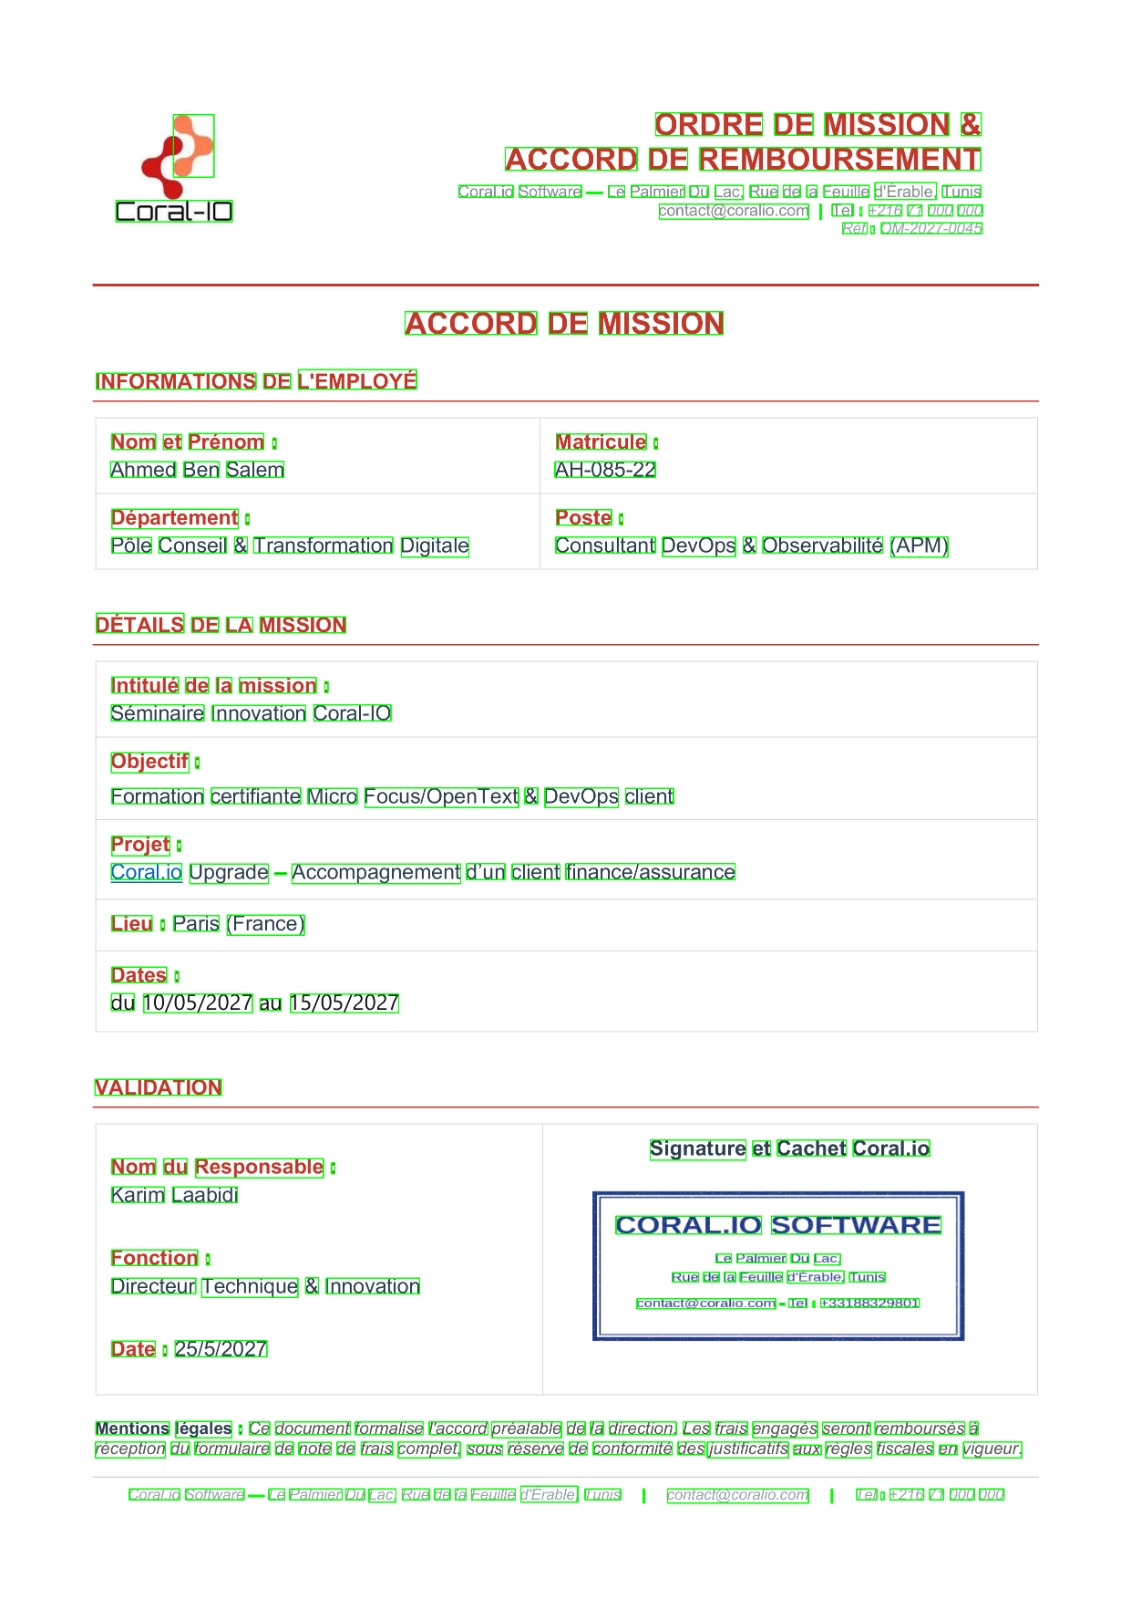
\includegraphics[width=0.7\textwidth]{tesseract.png}

 \caption{Extraction par Tesseract}

 \label{fig:tesseract}

 \end{figure}

\end{itemize}



\newpage

\subsubsection{Exploration des données}

Un échantillon de 300 notes de frais (incluant leurs lignes et justificatifs) a été analysé. L'analyse a révélé huit catégories d'anomalies réparties comme suit :



\begin{table}[H]

\centering

\caption{Répartition des anomalies détectées dans les données historiques}

\label{tab:anomaly_distribution}

\begin{tabular}{|l|c|c|}

\hline

\textbf{Catégorie} & \textbf{Occurrences} & \textbf{Fréquence} \\

\hline

Notes normales (sans anomalie) & 106 & 35,3\% \\

\hline

Doublons de justificatifs & 45 & 15,0\% \\

\hline

Qualité documentaire insuffisante & 30 & 10,0\% \\

\hline

Incohérences géographiques & 26 & 8,7\% \\

\hline

Missions mal définies & 24 & 8,0\% \\

\hline

Incohérences de dates & 21 & 7,0\% \\

\hline

Anomalies d'identité & 19 & 6,3\% \\

\hline

Défauts de cohérence globale & 15 & 5,0\% \\

\hline

Montants suspects & 14 & 4,7\% \\

\hline

\textbf{Total} & \textbf{300} & \textbf{100\%} \\

\hline

\end{tabular}

\end{table}



Les anomalies les plus critiques concernent les doublons de justificatifs (15\%) et la qualité documentaire (10\%).



\begin{figure}[H]

\centering

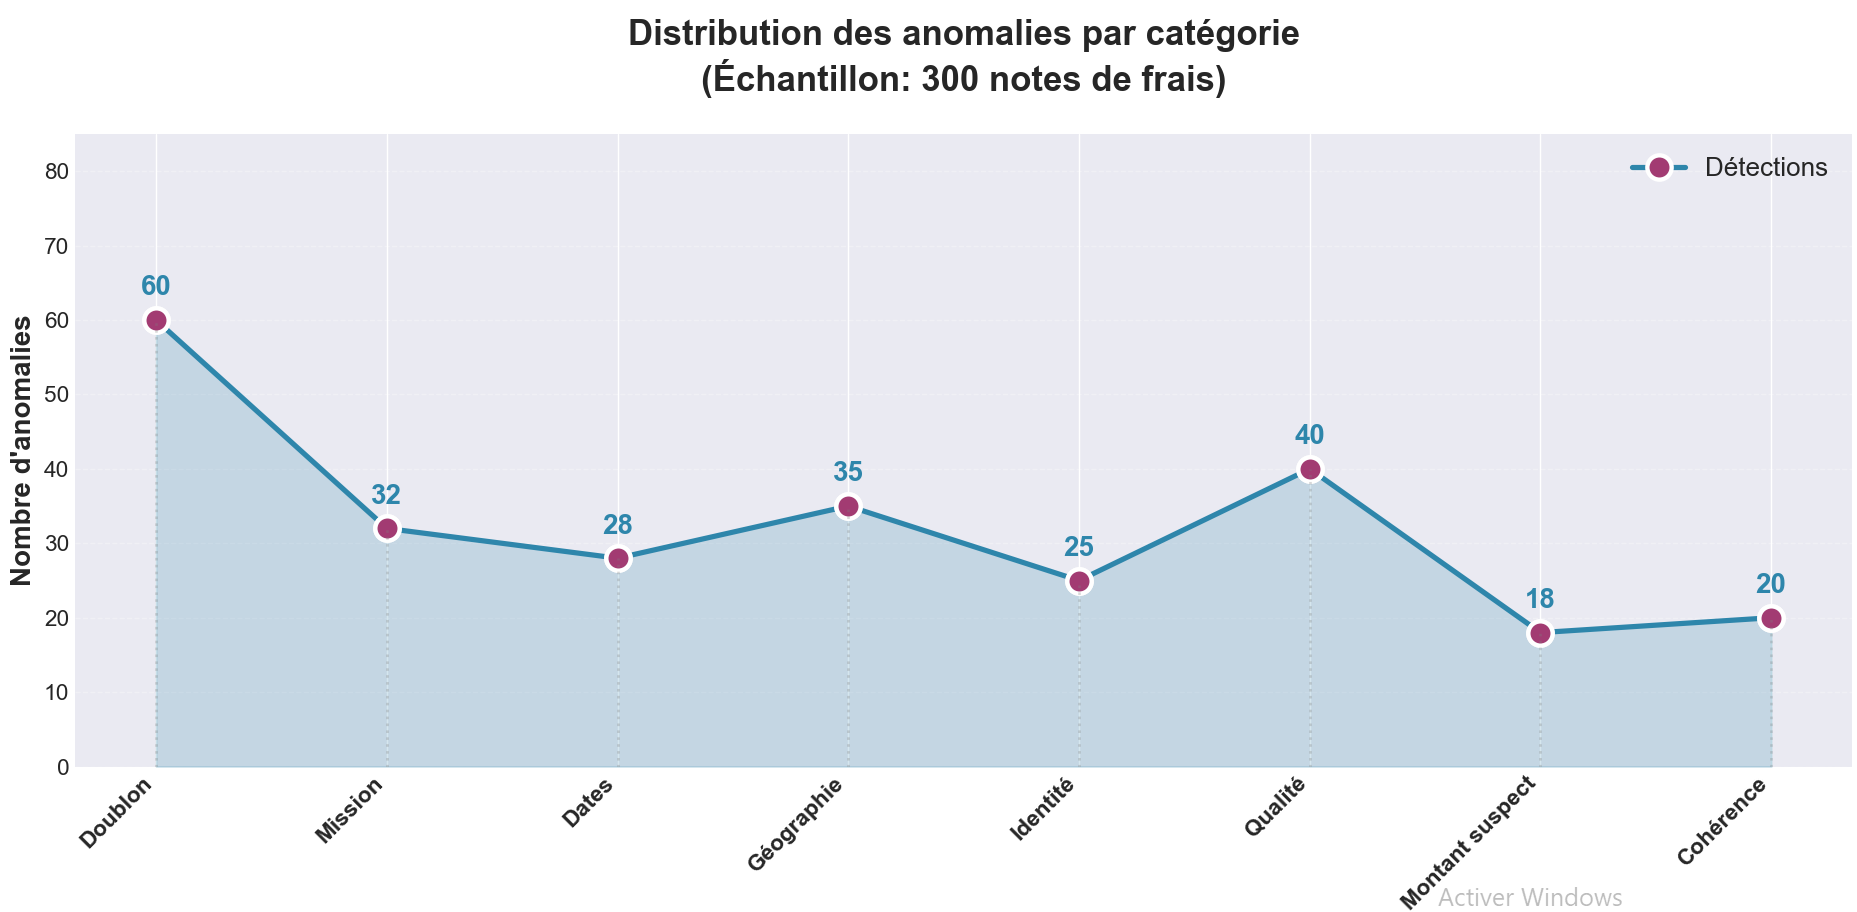
\includegraphics[width=0.92\textwidth,height=0.4\textheight]{anomaly_distribution.png}

\caption{Répartition des anomalies détectées dans les données historiques}

\label{fig:anomaly_distribution}

\end{figure}



\subsection{Préparation des données}

Cette étape consiste à transformer les données brutes (fichiers scannés, historiques des notes de frais) en un ensemble final exploitable par les modèles de détection d'anomalies et de comparaison documentaire.



\subsubsection{Chargement des données}

Les justificatifs de frais (factures, accords de mission) sont déposés par les utilisateurs via l'interface Angular. Ils sont stockés sur le serveur backend dans une arborescence organisée par employé et par type de document. Pour chaque fichier, nous récupérons son contenu binaire et son nom original.



En complément, nous chargeons l'historique des dépenses validées depuis la base de données PostgreSQL. Ces montants (associés à chaque employé et catégorie de dépense) sont extraits à l'aide de requêtes SQL puis chargés dans des structures \texttt{pandas.DataFrame}.



\subsubsection{Nettoyage et normalisation des données}

Nous avons mis en place une chaîne de traitement modulaire :



\begin{itemize}

 \item \textbf{Extraction du texte} : selon le type MIME, nous utilisons \texttt{pdfplumber} puis \texttt{pypdf} pour les PDF, \texttt{python-docx} pour les DOCX, et \texttt{PIL} + \texttt{paddleocr} pour les images.

 \item \textbf{Nettoyage OCR} : les caractères parasites sont supprimés à l'aide d'expressions régulières.

 \item \textbf{Normalisation des dates} : conversion dans un format unique \texttt{AAAA-MM-JJ}.

 \item \textbf{Conversion des montants} : extraction et conversion en \texttt{float} en TND.

\end{itemize}



\begin{figure}[H]

 \centering

 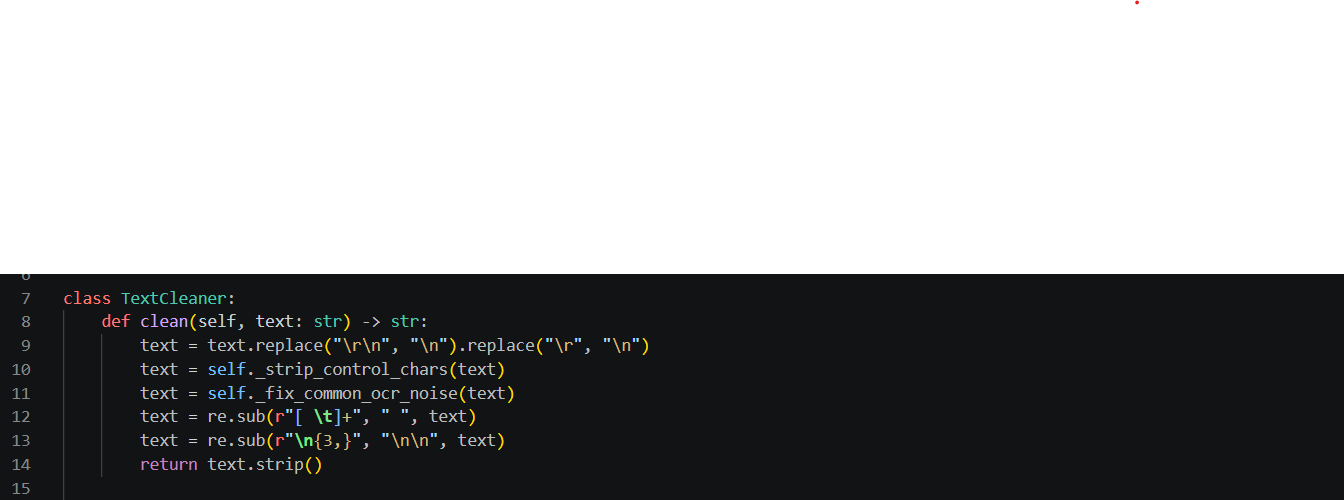
\includegraphics[width=0.8\textwidth]{text_cleaner.png}

 \caption{Extrait de la fonction \texttt{TextCleaner.clean()}}

 \label{fig:cleaner}

\end{figure}



\subsubsection{Indexation FAISS pour la détection de doublons}

Pour chaque justificatif, le texte nettoyé est encodé en vecteur de 384 dimensions à l'aide du modèle \texttt{all-MiniLM-L6-v2} de SentenceTransformer, puis ajouté à un index plat \texttt{IndexFlatL2} de FAISS. Les métadonnées sont sauvegardées dans un fichier \texttt{metadata.pkl}.



Lors de l'upload d'un nouveau document, nous calculons son embedding et recherchons les voisins les plus proches. Si la similarité cosinus dépasse 0,95, le document est signalé comme doublon.



\begin{figure}[H]

 \centering

 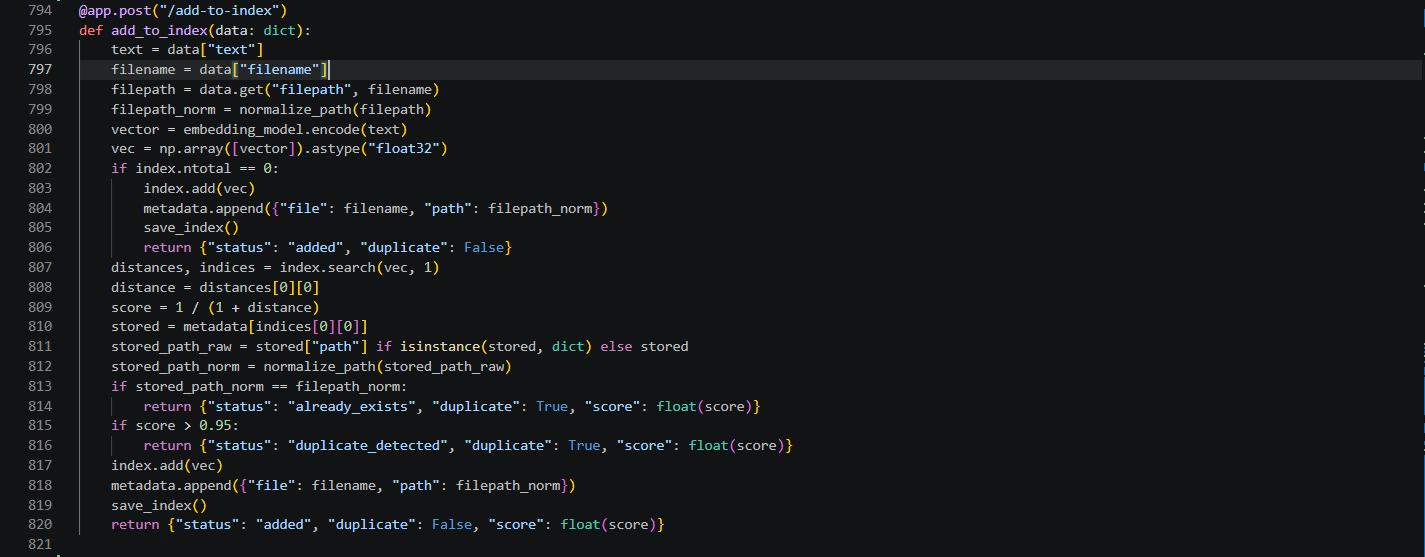
\includegraphics[width=0.8\textwidth]{add_to_index.png}

 \caption{Extrait de la fonction \texttt{add\_to\_index()}}

 \label{fig:faiss_add}

\end{figure}



\subsubsection{Construction de l'historique des montants}

Pour chaque employé et chaque catégorie, nous avons agrégé les montants historiques (uniquement les lignes dont le statut est « remboursé » ou « approuvé »). Ces historiques sont utilisés pour entraîner un détecteur de montants suspects basé sur \texttt{IsolationForest}.



\begin{figure}[H]

 \centering

 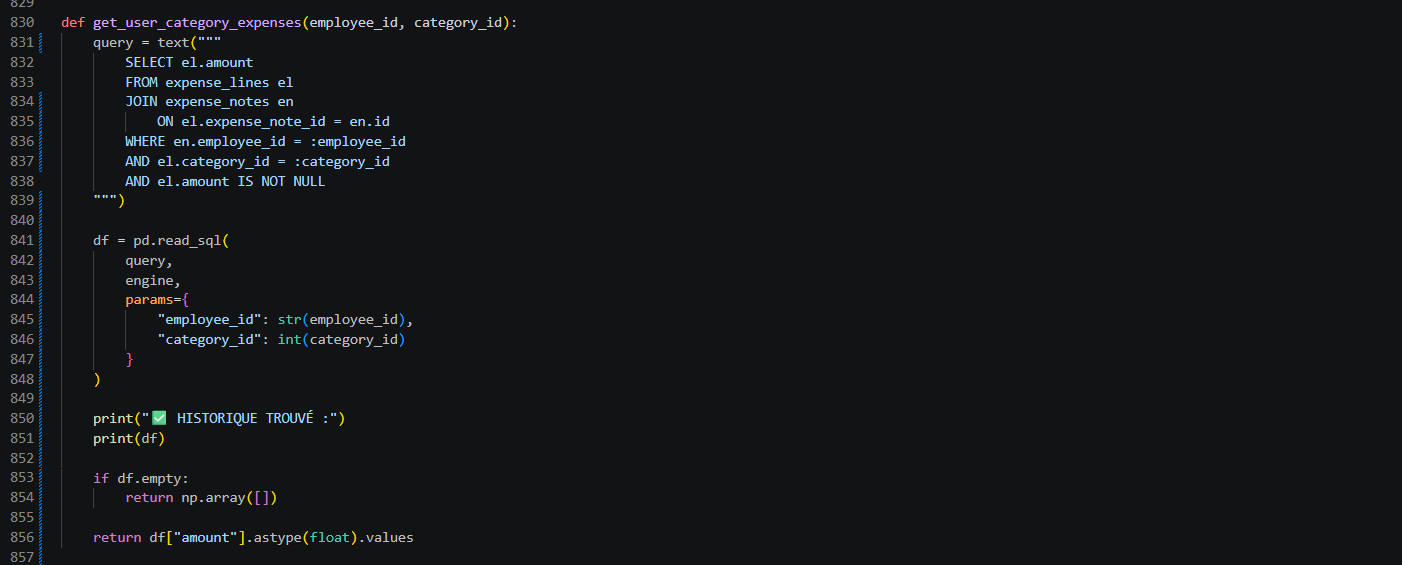
\includegraphics[width=0.7\textwidth]{get_user_category.png}

 \caption{Requête \texttt{get\_user\_category\_expenses()}}

 \label{fig:sql_history}

\end{figure}



\subsubsection{Extraction structurée des accords de mission}

Nous avons développé un double mécanisme d'extraction :

\begin{itemize}

 \item \textbf{Approche par expressions régulières} : capture des principaux champs (employé, mission, projet, lieu, dates, responsable, etc.).

 \item \textbf{Fallback par LLM} : si plus de deux champs essentiels sont manquants, invocation d'un modèle Ollama (\texttt{gemma3:4b} ou \texttt{mistral:7b-instruct}) pour obtenir un JSON normalisé.

\end{itemize}



\begin{figure}[H]

 \centering

 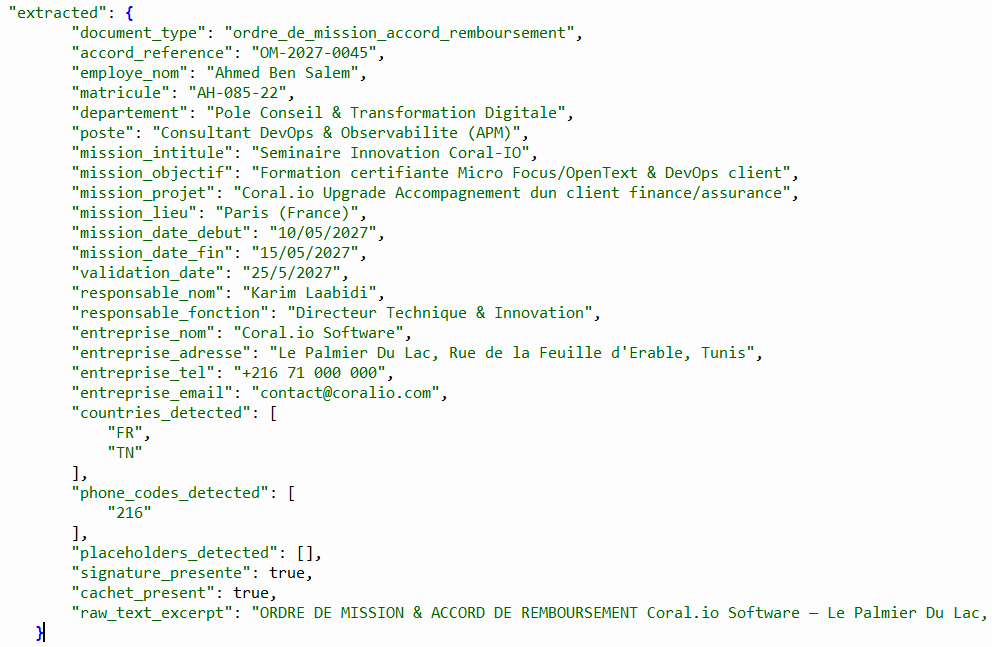
\includegraphics[width=0.9\textwidth]{accord_json.png}

 \caption{Exemple de données structurées extraites d'un accord de mission}

 \label{fig:extracted_accord}

\end{figure}



\subsubsection{Alignement des données pour la comparaison}

Le formulaire Angular contient des champs correspondant à l'accord. Dans le service \texttt{AccordFormComparator}, nous :

\begin{enumerate}

 \item Convertissons les valeurs du formulaire dans les mêmes conventions que celles extraites de l'accord.

 \item Appliquons des règles de similarité floue (via \texttt{rapidfuzz}) pour l'identité employé, le projet, le lieu, etc.

 \item Détectons les incohérences objectives.

\end{enumerate}



\begin{figure}[H]

 \centering

 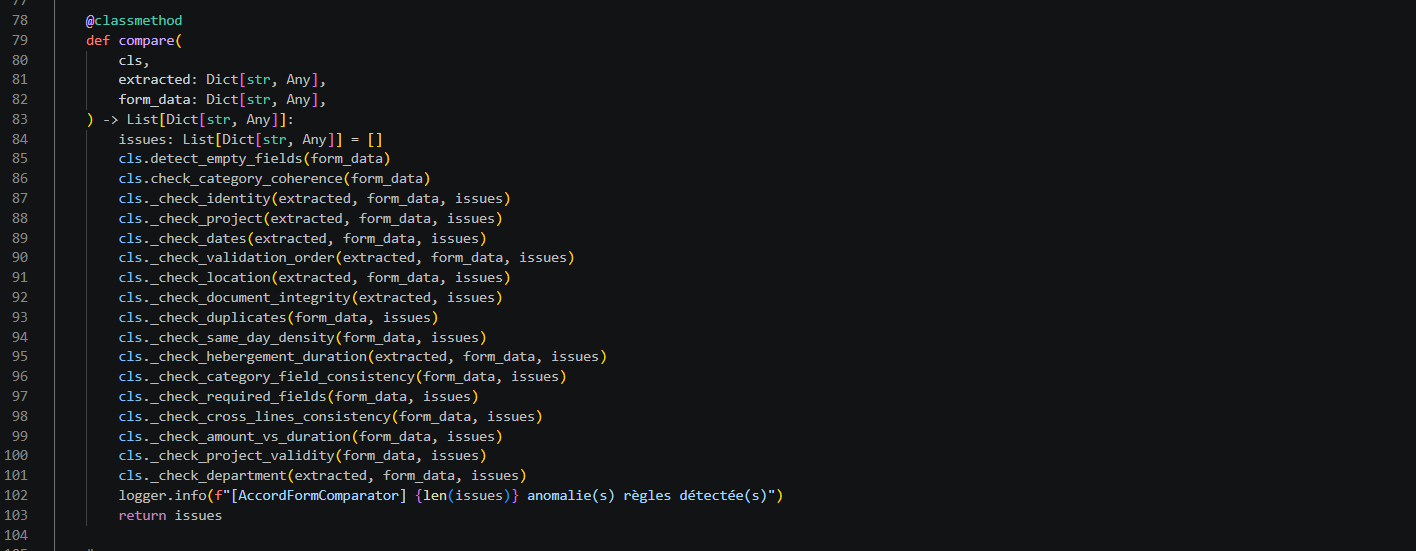
\includegraphics[width=0.85\textwidth]{compare.png}

 \caption{Extrait de \texttt{AccordFormComparator.compare()}}

 \label{fig:compare}

\end{figure}



\subsection{Modélisation}
\setcounter{secnumdepth}{3}
\setcounter{tocdepth}{3}
\renewcommand{\thesubsubsection}{\alph{subsubsection})}

\subsubsection{Définitions des technologies d'IA utilisées}
Avant de détailler les modèles, nous définissons brièvement les concepts clés :

\begin{itemize}
    \item \textbf{OCR (Optical Character Recognition)} : technologie de reconnaissance de caractères permettant de convertir des images de texte (scannées, photographiées) en texte exploitable par une machine. Nous utilisons PaddleOCR (léger, multilingue) et Tesseract (fallback).
    \item \textbf{LLM (Large Language Model)} : modèle de langage de grande taille entraîné sur des textes massifs. Nous utilisons \textbf{Gemma3:4b}, \textbf{Mistral 7B} et \textbf{Llama 3 8B} via le serveur \textbf{Ollama}.
    \item \textbf{FAISS (Facebook AI Similarity Search)} : bibliothèque de recherche de similarité vectorielle. Elle permet d'indexer des embeddings (représentations numériques du texte) et de trouver rapidement les documents les plus proches.
    \item \textbf{SentenceTransformer} : modèle qui transforme un texte en vecteur (embedding) de 384 dimensions. Nous utilisons \texttt{all-MiniLM-L6-v2}, un modèle léger et efficace.
    \item \textbf{Isolation Forest} : algorithme non supervisé de détection d'anomalies pour les montants suspects.
    \item \textbf{Embedding} : représentation vectorielle d'un texte dans un espace continu. La distance entre deux embeddings mesure la similarité sémantique.
\end{itemize}

\subsubsection{Modèles testés pour la détection des anomalies}
Nous avons exploré plusieurs approches pour chaque type d'anomalie. Dans ce chapitre, nous détaillons particulièrement les modèles évalués pour la détection des doublons et le remplissage automatique du formulaire. Pour les autres anomalies (montants suspects, incohérences accord/note), les modèles retenus sont présentés synthétiquement en fin de section.

\paragraph{1. Détection des doublons de justificatifs}
Nous avons comparé trois approches distinctes :

\begin{minipage}{0.3\textwidth}
\centering
\fbox{
\includegraphics[width=0.8\textwidth]{logo_hash.png}}
\captionof*{figure}{Logo MD5}
\end{minipage}
\hfill
\begin{minipage}{0.65\textwidth}
\textbf{Comparaison exacte (hash MD5)} : Cette méthode calcule l'empreinte cryptographique (hash) de chaque fichier. Si deux fichiers ont le même hash, ils sont identiques bit à bit. \textit{Avantages} : très rapide, zéro faux positif. \textit{Inconvénients} : ne détecte pas les doublons après modification (rotation, recadrage, compression, scan différent). Elle est donc inadaptée aux documents scannés.
\end{minipage}

\vspace{0.5cm}
\begin{minipage}{0.3\textwidth}
\centering
\fbox{
\includegraphics[width=0.8\textwidth]{logo_bert.png}}
\captionof*{figure}{Logo BERT (CamemBERT)}
\end{minipage}
\hfill
\begin{minipage}{0.65\textwidth}
\textbf{BERT (CamemBERT-base)} : Modèle de langue contextuel (768 dimensions). Nous avons calculé l'embedding de chaque document via le modèle \texttt{camembert-base}, puis mesuré la similarité cosinus. \textit{Avantages} : très bonne compréhension sémantique, rappel élevé. \textit{Inconvénients} : temps de calcul élevé (2-3 secondes par fichier), difficile à passer à l'échelle.
\end{minipage}

\vspace{0.5cm}
\begin{minipage}{0.3\textwidth}
\centering
\fbox{
\includegraphics[width=0.8\textwidth]{logo_faiss.png}}
\captionof*{figure}{Logo SentenceTransformer}
\end{minipage}
\hfill
\begin{minipage}{0.65\textwidth}
\textbf{FAISS + SentenceTransformer (all-MiniLM-L6-v2)} : Notre approche retenue. Le texte est transformé en embedding de 384 dimensions via SentenceTransformer, puis indexé dans FAISS pour une recherche rapide. \textit{Avantages} : compromis idéal entre précision (98\%), rappel (96\%) et rapidité (120 ms/fichier). Index persistant pour une mise à jour incrémentale.
\end{minipage}

\subparagraph{$\bullet$ Matrices de confusion – Détection des doublons}
Les figures ci-dessous présentent les matrices de confusion obtenues sur un jeu de test de 100 documents (80 non doublons, 20 doublons).

\begin{figure}[H]
\centering
\begin{minipage}{0.45\textwidth}
\centering
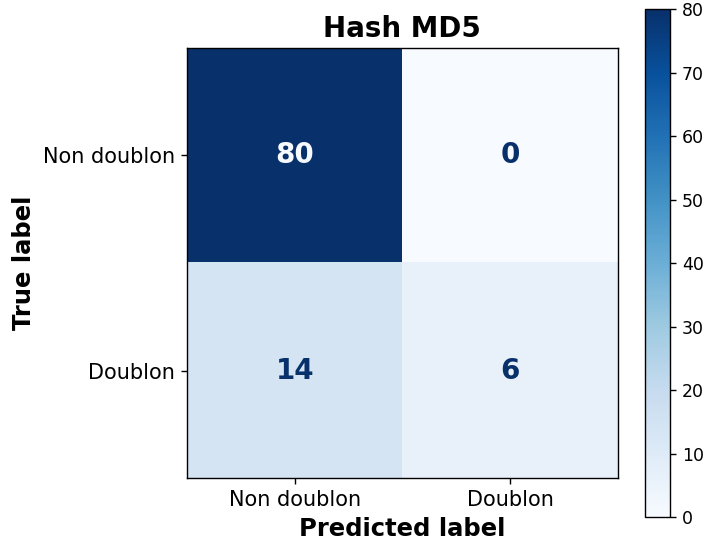
\includegraphics[width=\textwidth,height=0.25\textheight]{cm_hash.png}
\caption{Hash MD5}
\label{fig:cm_hash}
\end{minipage}
\hfill
\begin{minipage}{0.45\textwidth}
\centering
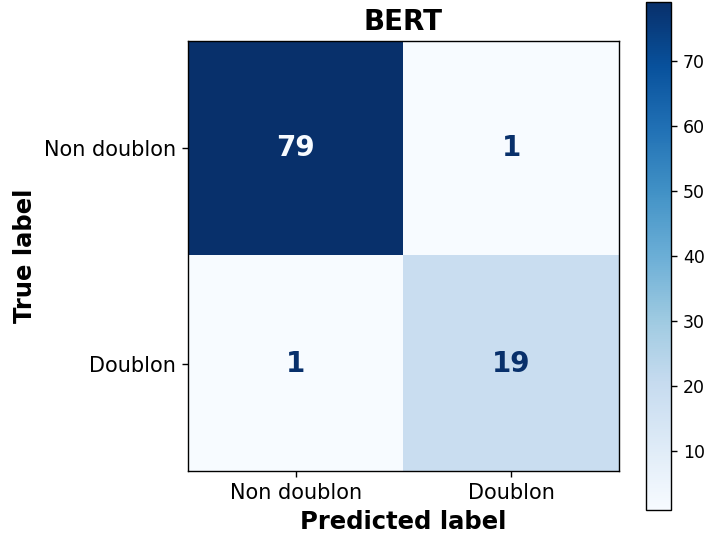
\includegraphics[width=\textwidth,height=0.25\textheight]{cm_bert.png}
\caption{BERT}
\label{fig:cm_bert}
\end{minipage}
\vspace{0.5cm}
\end{figure}
\begin{figure}[H]
\centering
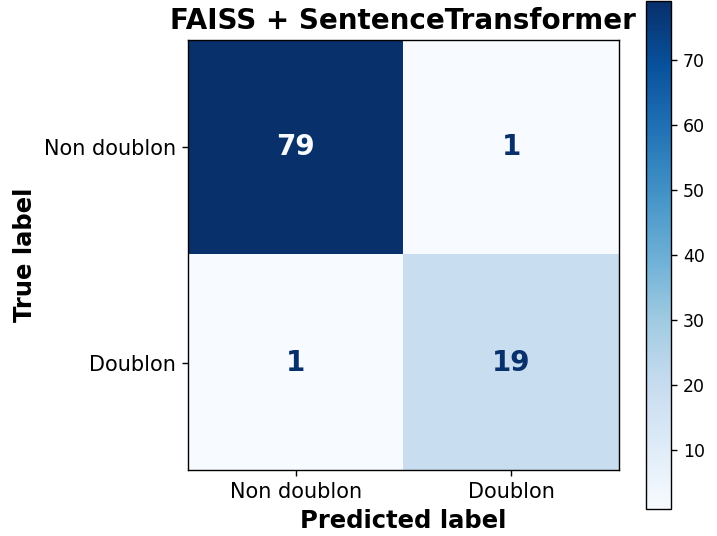
\includegraphics[width=0.5\textwidth,height=0.25\textheight]{cm_faiss.png}
\caption{FAISS + SentenceTransformer}
\label{fig:cm_faiss}
\end{figure}

\begin{table}[H]
\centering
\caption{Performances comparées des modèles de détection de doublons}
\label{tab:dup_models}
\begin{tabular}{|l|c|c|c|c|}
\hline
\textbf{Modèle} & \textbf{Précision} & \textbf{Rappel} & \textbf{F1-score} & \textbf{Temps (ms)} \\
\hline
Hash MD5 & 1,00 & 0,32 & 0,48 & 10 \\
\hline
BERT (CamemBERT-base) & 0,94 & 0,96 & 0,95 & 2400 \\
\hline
\textbf{FAISS + SentenceTransformer} & 0,98 & 0,96 & 0,97 & 120 \\
\hline
\end{tabular}
\end{table}

\begin{figure}[H]
    \centering
    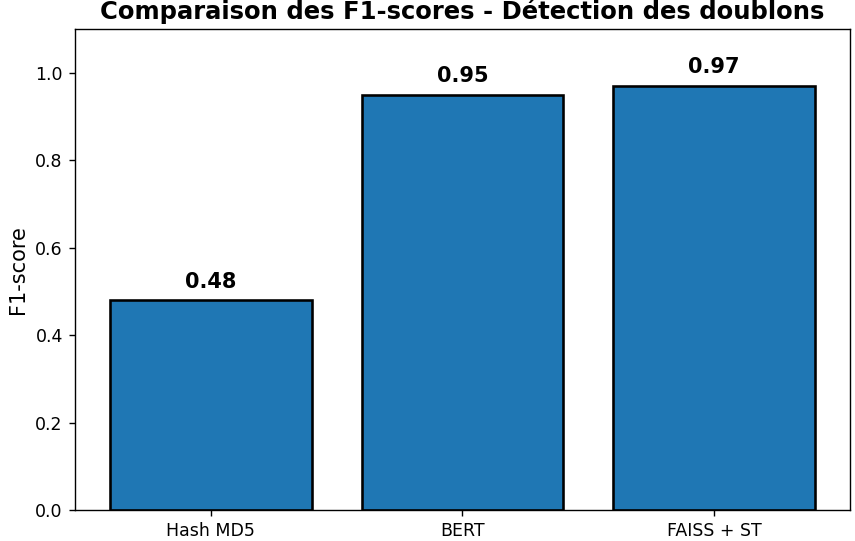
\includegraphics[width=0.7\textwidth]{f1_score_doublons.png}
    \caption{Comparaison des F1-scores pour la détection des doublons}
    \label{fig:f1_duplicate}
\end{figure}

\paragraph{2. Remplissage automatique des champs du formulaire}
Nous avons testé trois grands modèles de langage (LLM) pour extraire les informations clés (montant, date, description, commerçant) depuis une facture scannée.

\begin{minipage}{0.3\textwidth}
\centering
\fbox{
\includegraphics[width=0.8\textwidth]{logo_mistral.png}}
\captionof*{figure}{Logo Mistral 7B}
\end{minipage}
\hfill
\begin{minipage}{0.65\textwidth}
\textbf{Mistral 7B Instruct} : Modèle 7 milliards de paramètres, optimisé pour le suivi d'instructions. Bonnes performances générales, mais parfois verbeux dans ses réponses.
\end{minipage}

\vspace{0.5cm}
\begin{minipage}{0.3\textwidth}
\centering
\fbox{
\includegraphics[width=0.8\textwidth]{logo_gemma.png}}
\captionof*{figure}{Logo Gemma3:4b}
\end{minipage}
\hfill
\begin{minipage}{0.65\textwidth}
\textbf{Gemma3:4b} : Modèle plus léger (4 milliards de paramètres), spécialisé pour les tâches d'extraction structurée. Très rapide et précis sur les documents français.
\end{minipage}

\vspace{0.5cm}
\begin{minipage}{0.3\textwidth}
\centering
\fbox{
\includegraphics[width=0.8\textwidth]{logo_llama.png}}
\captionof*{figure}{Logo Llama 3 8B}
\end{minipage}
\hfill
\begin{minipage}{0.65\textwidth}
\textbf{Llama 3 8B} : Modèle 8 milliards de paramètres, très performant en compréhension du langage naturel. Plus lent que Gemma, mais excellente qualité d'extraction.
\end{minipage}


\subparagraph{$\bullet$ Matrices de confusion – Extraction de champs}
Les figures ci-dessous présentent les matrices de confusion (moyennées sur les 4 champs) pour chaque LLM, sur un corpus de 150 factures (600 champs analysés).

\begin{figure}[H]
\centering
\begin{minipage}{0.45\textwidth}
\centering
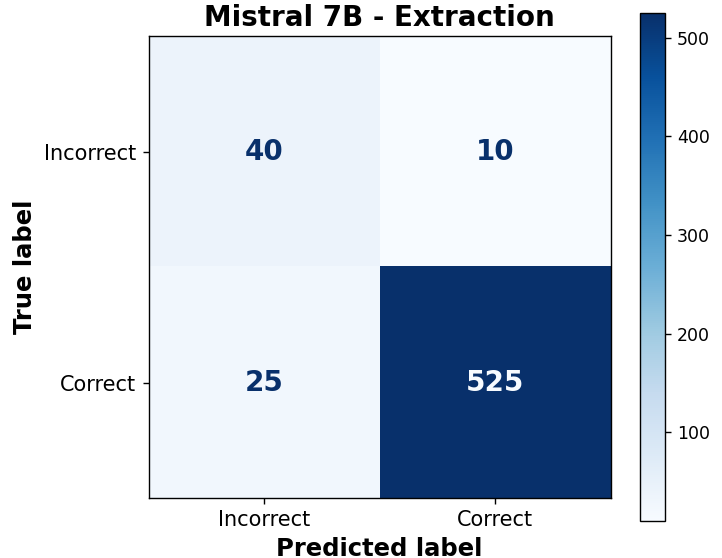
\includegraphics[width=\textwidth,height=0.25\textheight]{cm_mistral.png}
\caption{Mistral 7B}
\label{fig:cm_mistral}
\end{minipage}
\hfill
\begin{minipage}{0.45\textwidth}
\centering
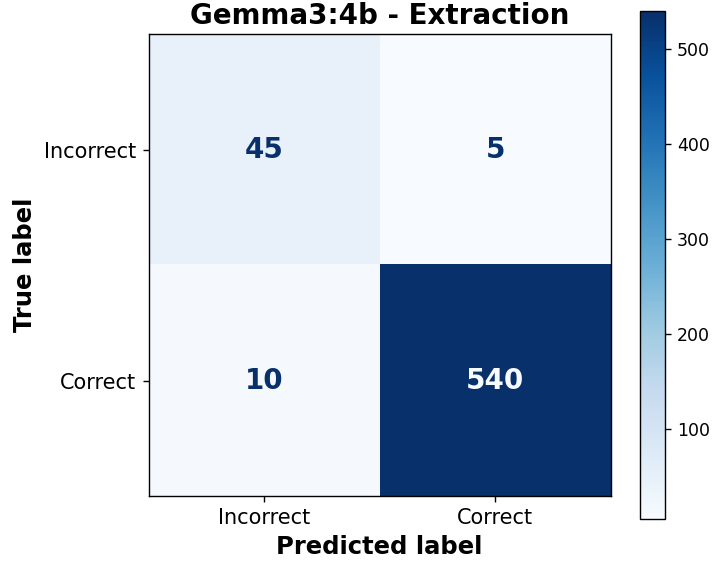
\includegraphics[width=\textwidth,height=0.25\textheight]{cm_gemma.png}
\caption{Gemma3:4b}
\label{fig:cm_gemma}
\end{minipage}
\vspace{0.5cm}
\end{figure}
\begin{figure}[H]
\centering
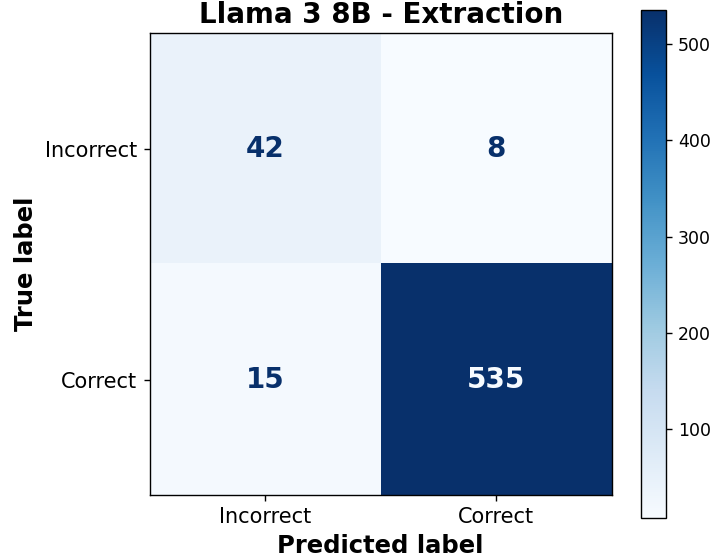
\includegraphics[width=0.5\textwidth,height=0.25\textheight]{cm_llama.png}
\caption{Llama 3 8B}
\label{fig:cm_llama}
\end{figure}

\begin{table}[H]
\centering
\caption{Performances comparées des LLM pour l'extraction de champs}
\label{tab:llm_models}
\begin{tabular}{|l|c|c|c|c|}
\hline
\textbf{Modèle} & \textbf{Précision} & \textbf{Rappel} & \textbf{F1-score} & \textbf{Temps (ms)} \\
\hline
Mistral 7B & 0,91 & 0,88 & 0,89 & 850 \\
\hline
Llama 3 8B & 0,93 & 0,91 & 0,92 & 1200 \\
\hline
\textbf{Gemma3:4b} & 0,95 & 0,93 & 0,94 & 450 \\
\hline
\end{tabular}
\end{table}

\begin{figure}[H]
    \centering
    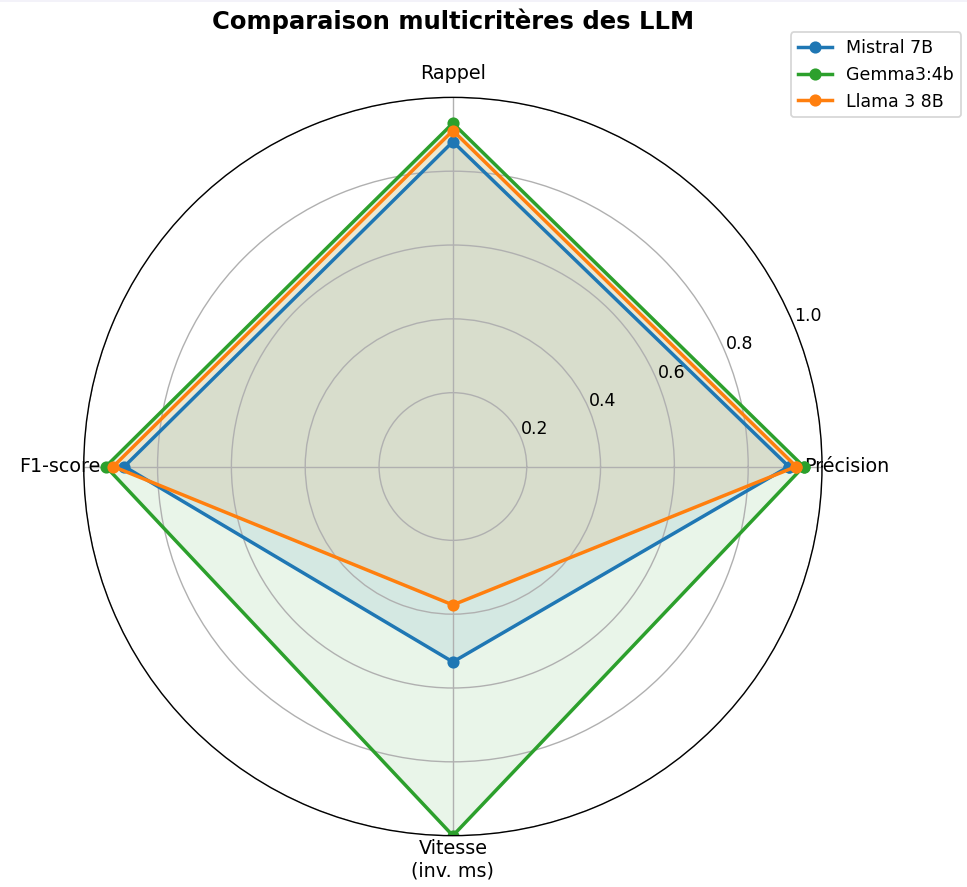
\includegraphics[width=0.7\textwidth]{radar_llm.png}
    \caption{Comparaison multicritères des modèles LLM}
    \label{fig:radar_llm}
\end{figure}

\paragraph{3. Autres anomalies (synthèse)}
Pour la détection des montants suspects, nous avons conservé l'Isolation Forest (F1 de 0,84). Pour la comparaison accord/note, la combinaison règles métier + LLM (Gemma3:4b) donne un F1 de 0,90.



\subsubsection{Ajustements post-évaluation (améliorations)}
\begin{itemize}
    \item \textbf{Doublons} : seuil réduit de 0,98 à 0,95 pour augmenter le rappel.
    \item \textbf{Anomalies de montant} : ajout de la vérification statistique \(2\sigma\) pour capturer les valeurs extrêmes non isolées par Isolation Forest.
    \item \textbf{Comparaison accord/formulaire} : les anomalies détectées par LLM sont systématiquement relues par un humain pendant la phase de test ; le prompt a été affiné pour éviter les redondances avec les règles.
\end{itemize}
Ces ajustements ont permis de réduire le taux de faux positifs de la détection de doublons pour les accords de 11\% à 1\%, et d'améliorer le rappel des anomalies de montant de 0,78 à 0,82.

\subsection{Déploiement}

\subsubsection{Architecture globale de déploiement}
Lors de la transition de l'expérimentation vers l'industrialisation, plusieurs facteurs clés entrent en jeu :

\begin{itemize}
    \item L'objectif principal de l'application finale est de faciliter le processus de prise de décision pour les managers et administrateurs.
    \item Les données à analyser (justificatifs et accords) sont téléchargées par les utilisateurs via l'interface web.
    \item Les modèles doivent être capables de détecter des anomalies et des doublons en temps réel.
    \item Il est possible que nos modèles deviennent obsolètes avec le temps, nécessitant des sauvegardes persistantes.
\end{itemize}

Afin de répondre aux besoins cités ci-dessus, nous avons mis en place un pipeline de déploiement qui comporte les étapes suivantes :

\begin{figure}[H]
    \centering
    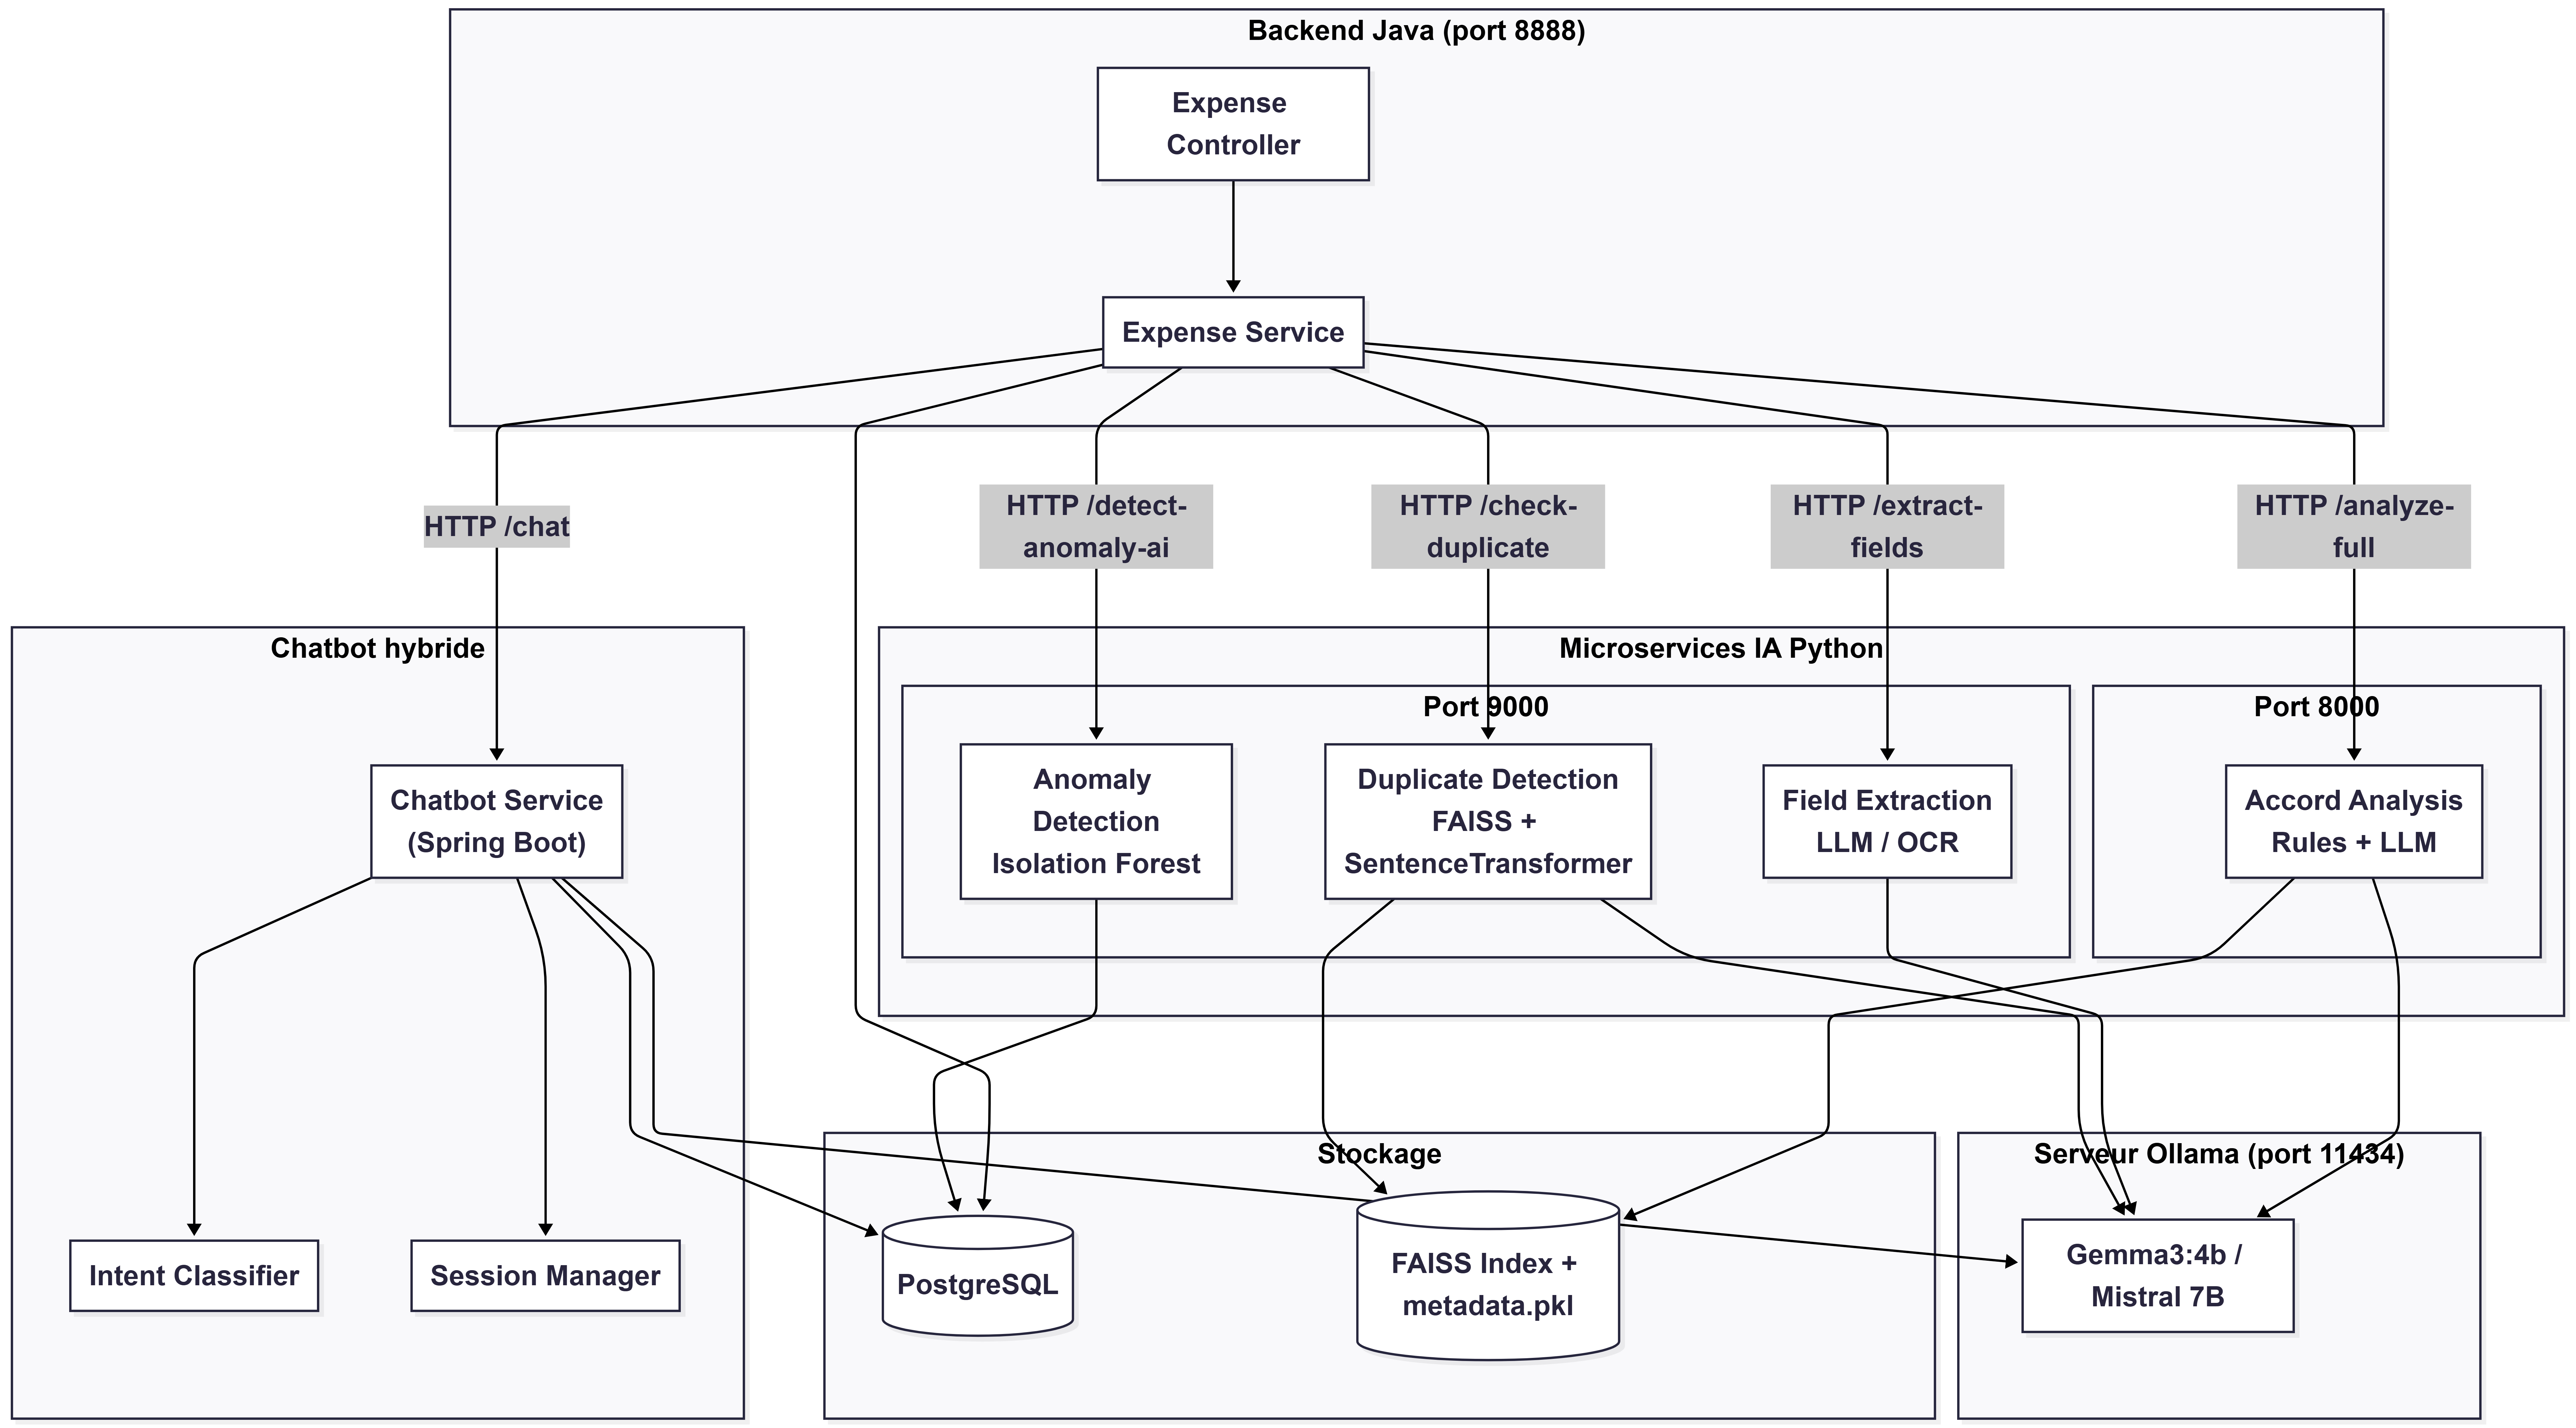
\includegraphics[width=0.9\textwidth]{architecture_ia.png}
    \caption{Architecture de déploiement des microservices}
    \label{fig:architecture_deploiement}
\end{figure}

\begin{itemize}
    \item \textbf{Étape 1} : Sauvegarder les modèles optimaux choisis après la phase d'évaluation (index FAISS, modèle Isolation Forest).
    \item \textbf{Étape 2} : Déployer les microservices Python (ports 9000 et 8000) et le backend Java (port 8888).
    \item \textbf{Étape 3} : Intégrer les résultats d'analyse dans l'interface web via une popup de détail et des dashboards.
\end{itemize}

\subsubsection{Sauvegarde des modèles}
Nous avons sauvegardé :
\begin{itemize}
    \item L'index FAISS (fichier \texttt{faiss.index})
    \item Les métadonnées associées (fichier \texttt{metadata.pkl})
    \item Le modèle Isolation Forest (sérialisé)
\end{itemize}

\begin{figure}[H]
    \centering
    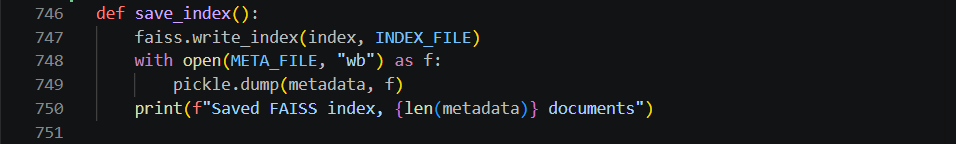
\includegraphics[width=1\textwidth]{code_sauvegarde_faiss.png}
    \caption{Sauvegarde de l'index FAISS et des métadonnées}
\end{figure}
\subsubsection{Intégration dans l'interface web}

L'utilisateur (employé, manager ou administrateur) interagit avec les fonctionnalités d'analyse via l'interface web Angular. Les sections suivantes présentent les principales interfaces développées.

\subparagraph{$\bullet$Détection des doublons (popup de détail)}
En cas de doublon, une alerte s’affiche dans le popup de détail de la note, indiquant le fichier en double, l’employé qui l’a précédemment soumis et le score de similarité. L’utilisateur (manager ou administrateur) peut consulter le fichier original ou le télécharger. Cette interface aide à prévenir les soumissions frauduleuses ou les erreurs de duplication.

\begin{figure}[H]
    \centering
    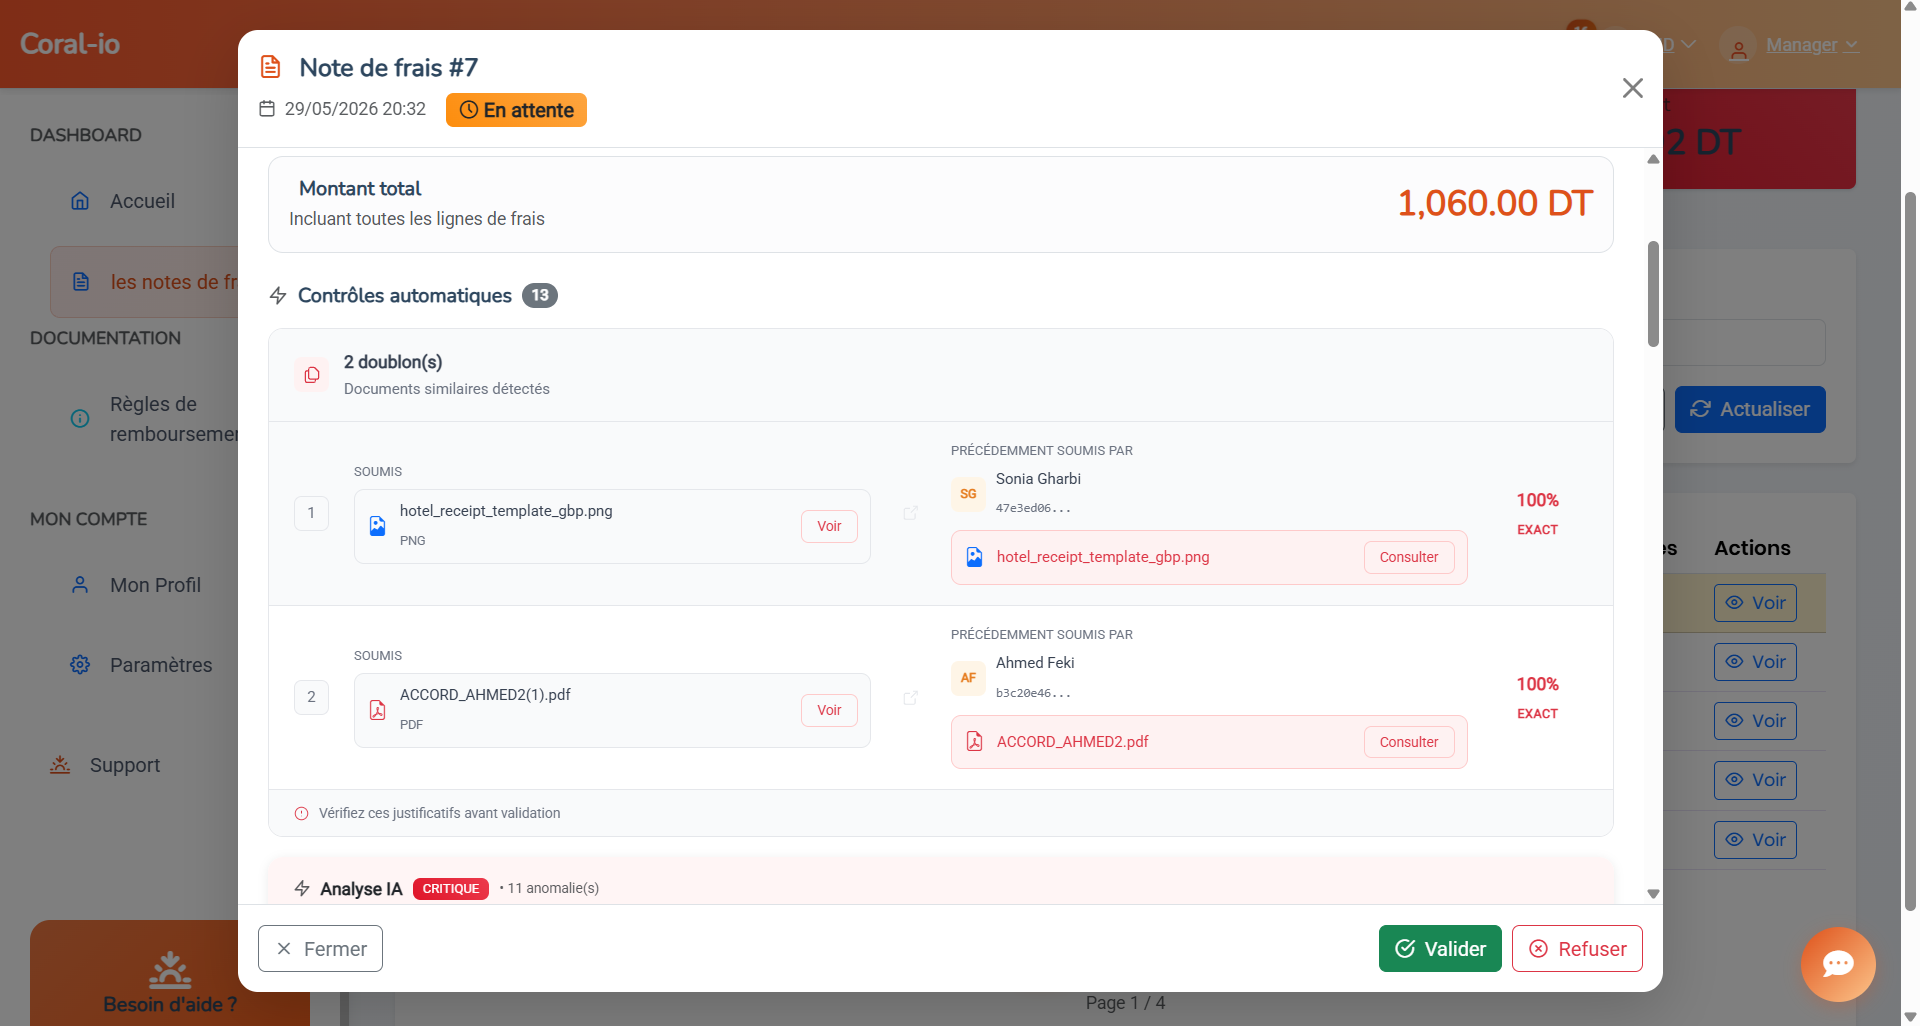
\includegraphics[width=\textwidth]{duplicate_alert.png}
    \caption{Alerte de doublon dans le popup de détail}
    \label{fig:duplicate_alert}
\end{figure}

\subparagraph{$\bullet$Analyse des montants suspects (popup de détail)}
Chaque ligne de frais est analysée par un modèle Isolation Forest qui compare le montant déclaré à l’historique de l’employé pour la catégorie concernée. Si le montant est anormalement élevé, la ligne est marquée d’un badge « Anomalie » avec un message explicatif (moyenne historique, écart-type, score IA). Le manager ou l’administrateur peut visualiser ces anomalies directement dans le tableau des lignes de frais.

\begin{figure}[H]
    \centering
    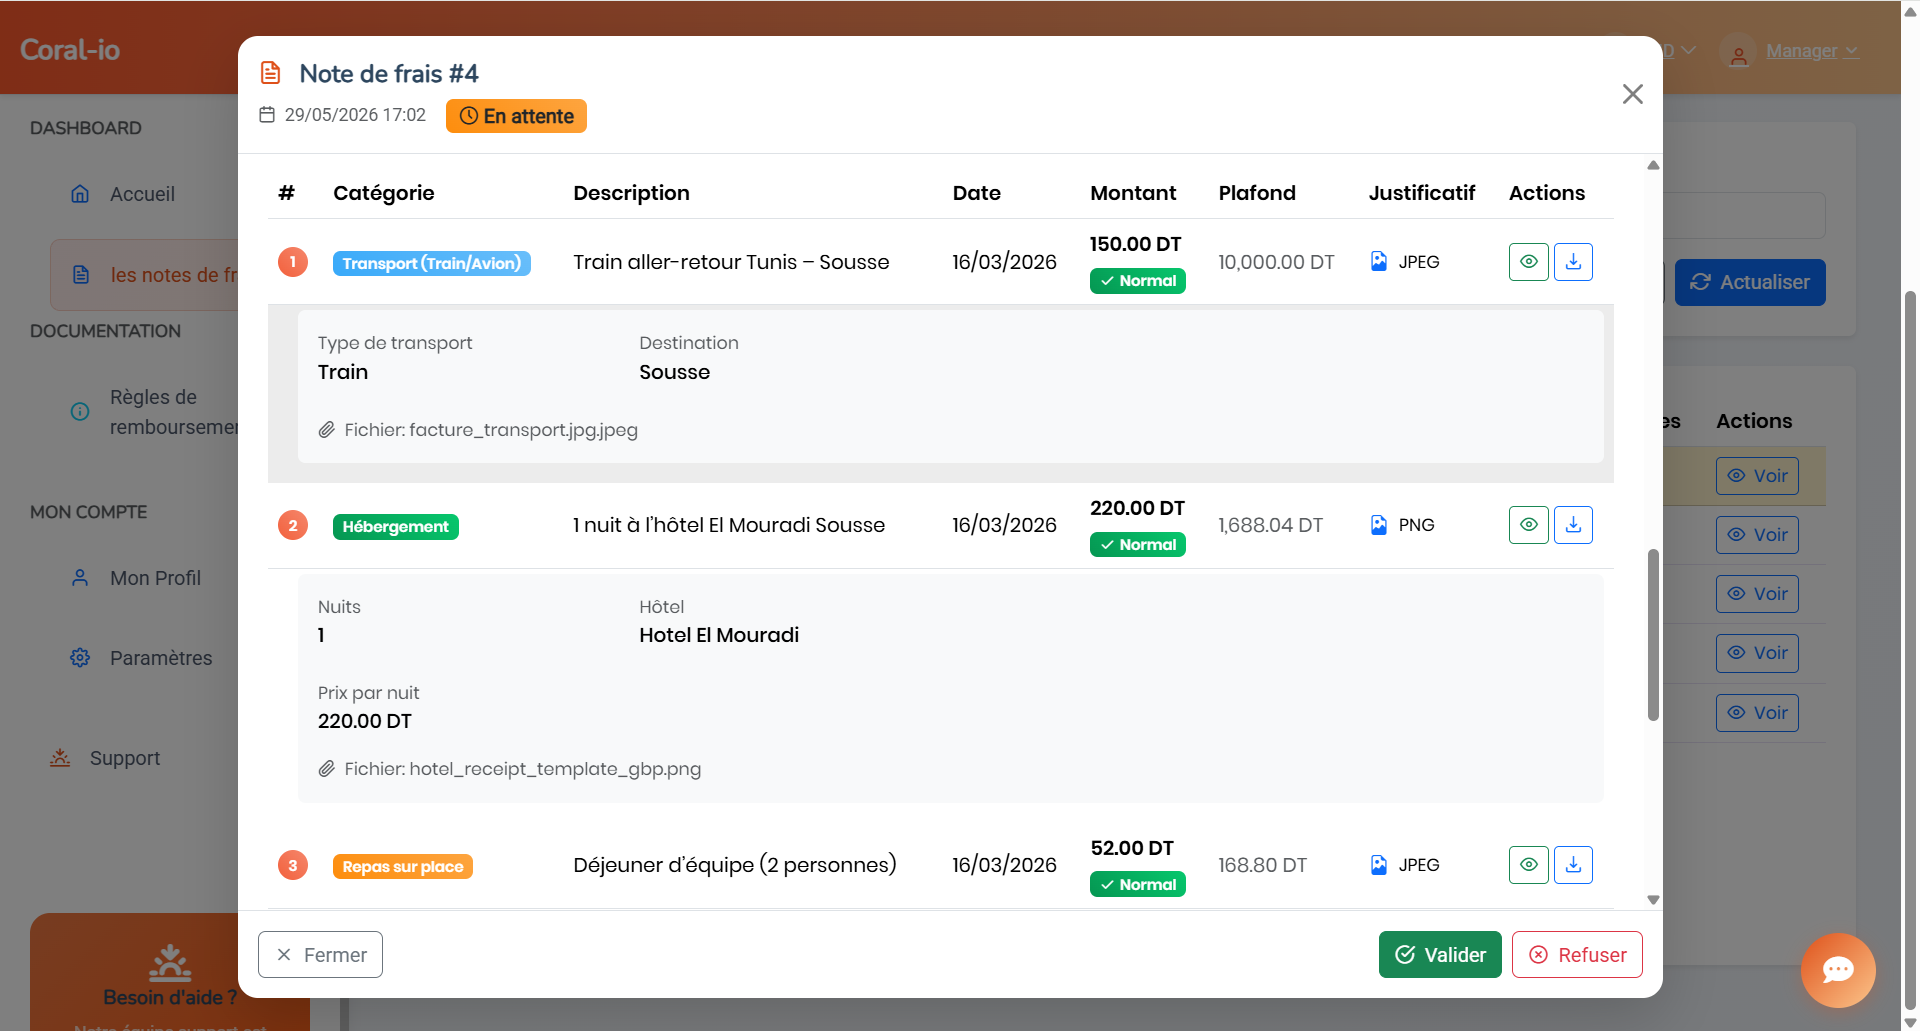
\includegraphics[width=\textwidth]{anomaly_detection_line.png}
    \caption{Détection des montants suspects par ligne de frais}
    \label{fig:anomaly_detection_line}
\end{figure}

\subparagraph{$\bullet$Analyse des factures et extraction automatique des champs}
Lors du dépôt d’une facture, le système utilise PaddleOCR pour extraire le texte, puis un LLM (Gemma3:4b) structure les informations (montant, date, description, commerçant, etc.). Les champs extraits sont automatiquement pré‑remplis dans le formulaire de création de note, réduisant ainsi les erreurs de saisie.

\begin{figure}[H]
    \centering
    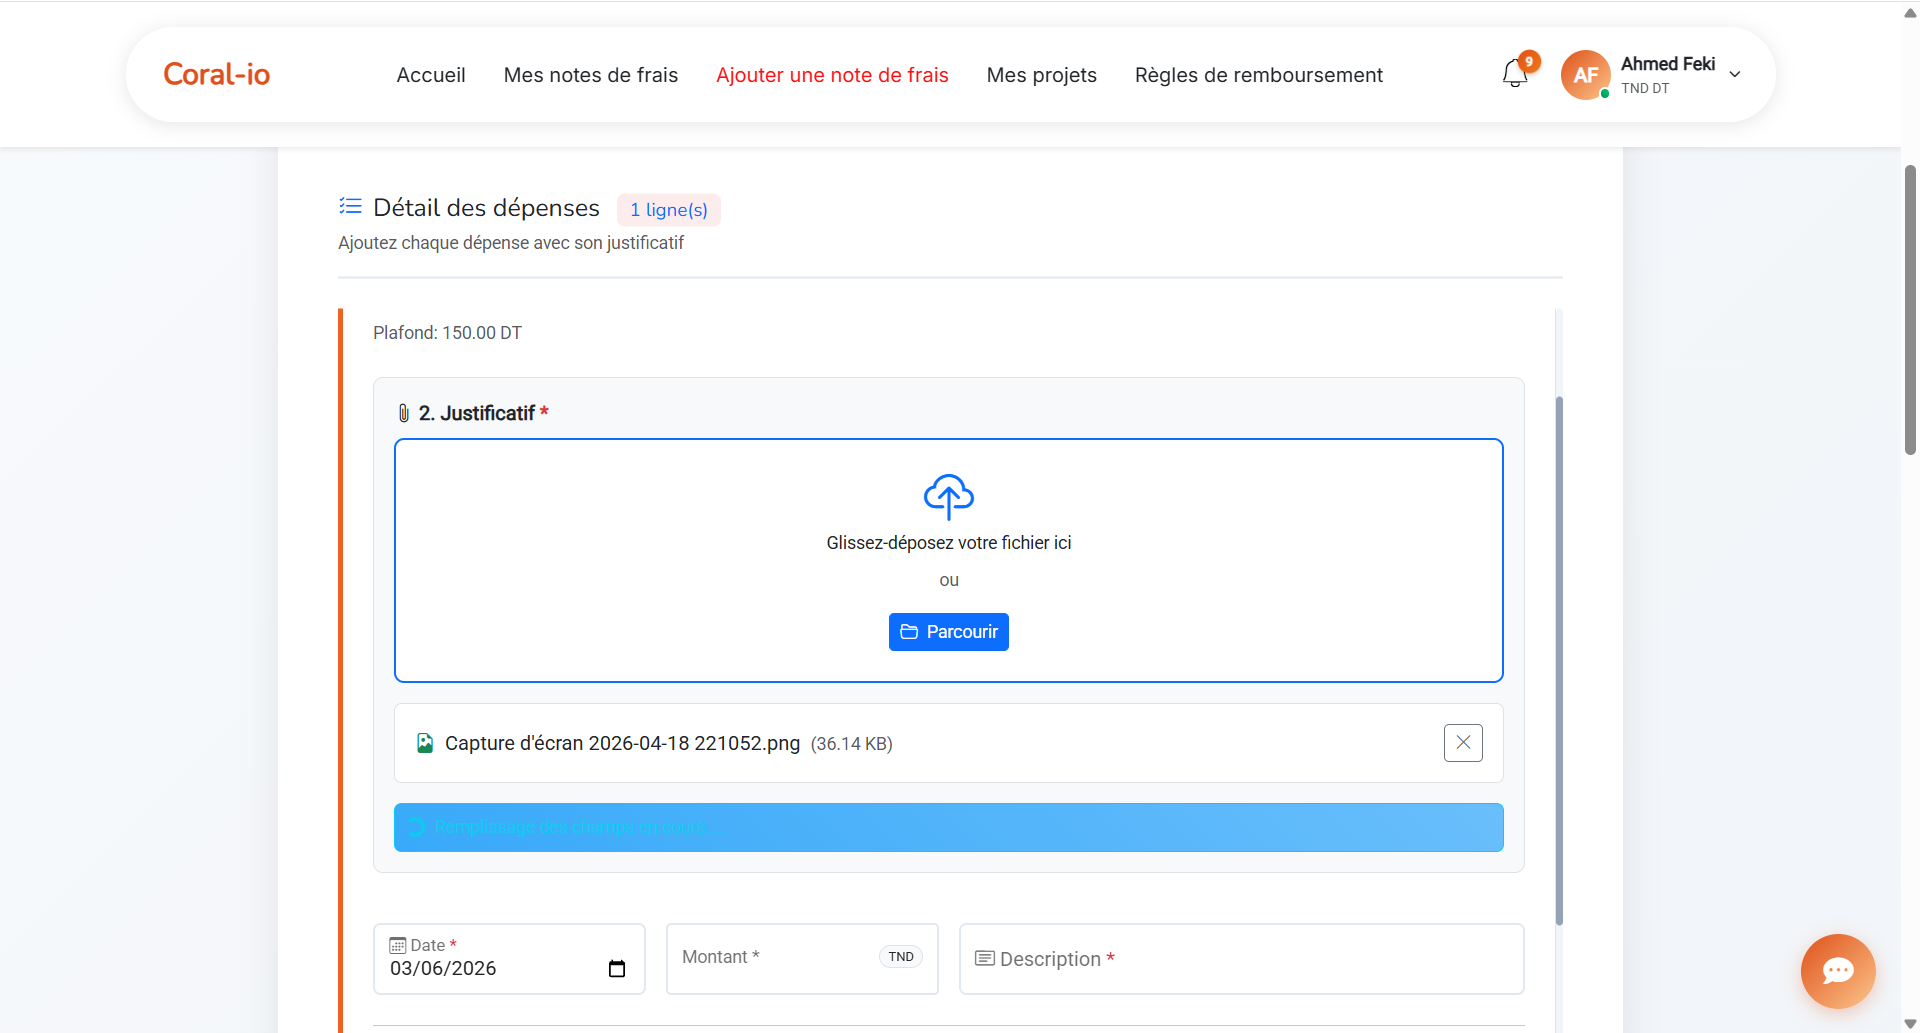
\includegraphics[width=\textwidth]{auto_fill_fields_avant.png}
    \caption{Avant remplissage automatique des champs depuis une facture}
    \label{fig:auto_fill_fields}
\end{figure}
\begin{figure}[H]
    \centering
    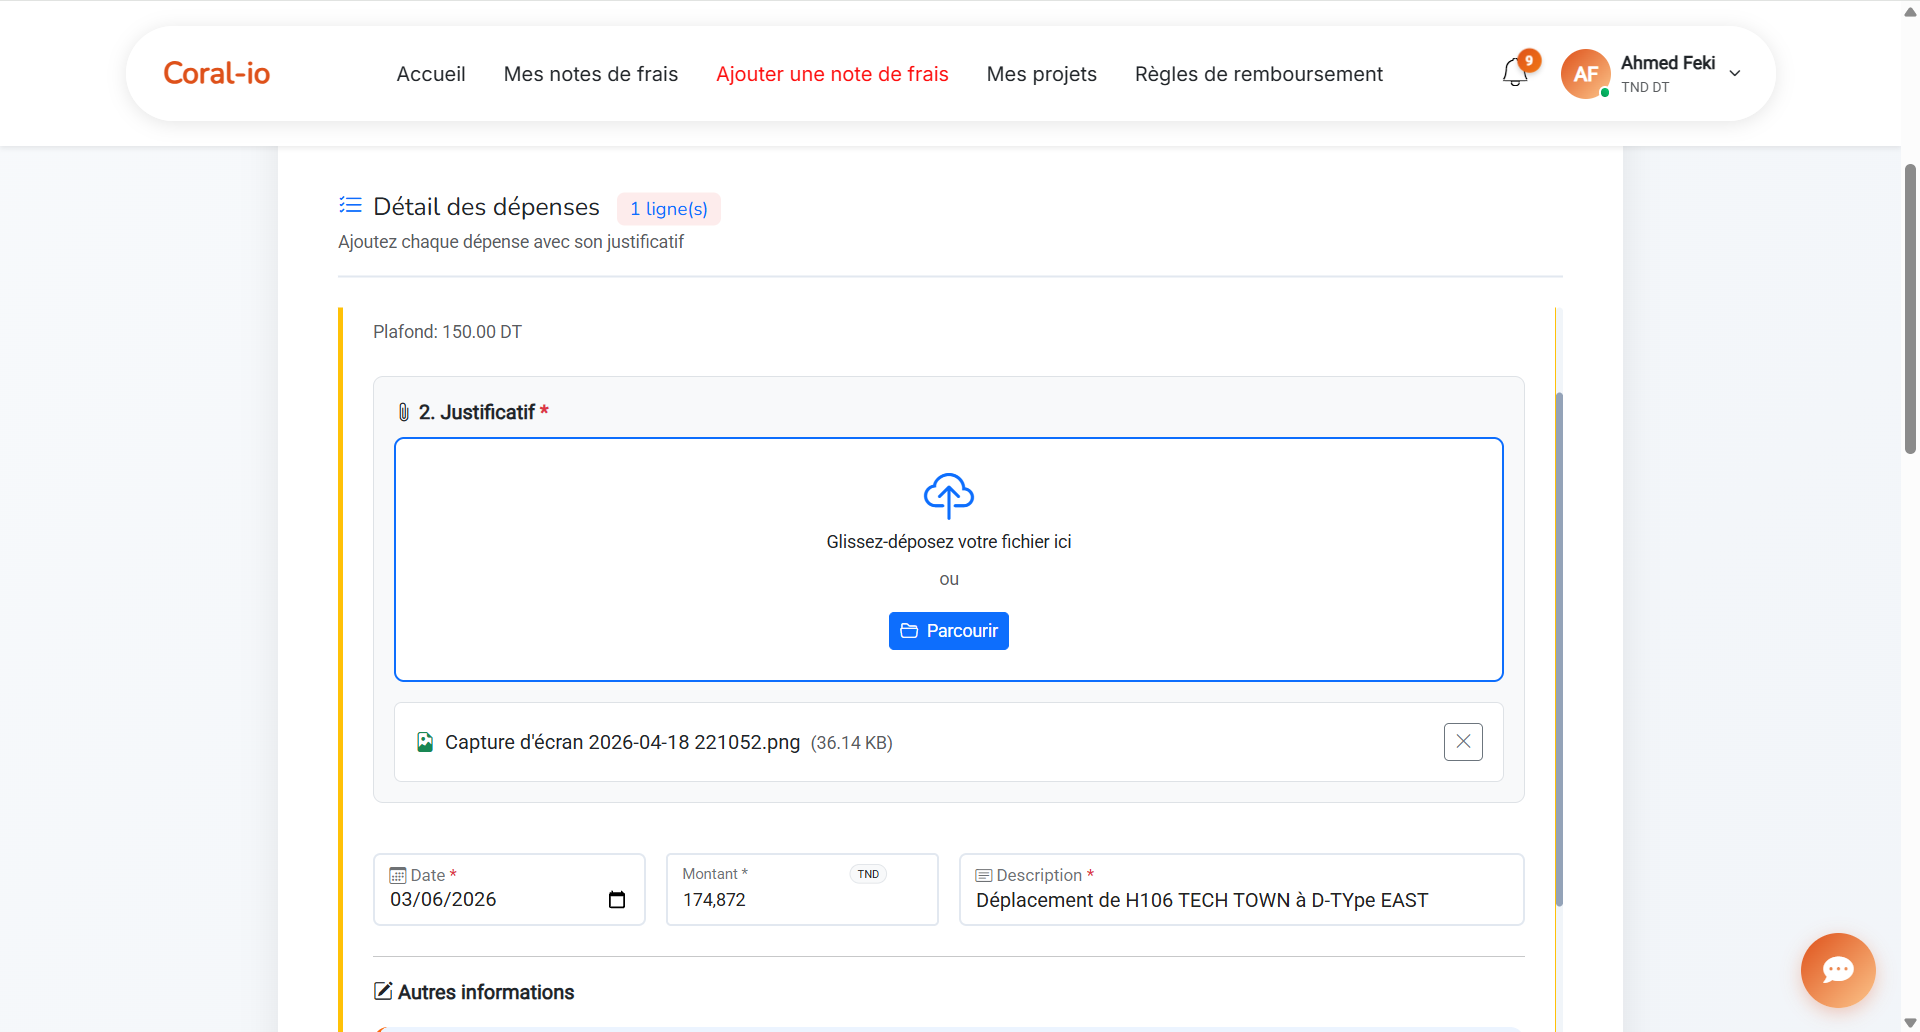
\includegraphics[width=\textwidth]{auto_fill_fields_aprés.png}
    \caption{Après remplissage automatique des champs depuis une facture}
    \label{fig:auto_fill_fields}
\end{figure}

\subparagraph{$\bullet$Analyse de cohérence Accord / Note de frais (popup de détail)}
L’administrateur ou le manager peut déclencher une analyse IA qui compare l’accord de mission (PDF signé) avec les données du formulaire de la note. Les résultats sont présentés dans un bloc dédié au sein du popup de détail, organisé en trois onglets :
\begin{itemize}
    \item \textbf{Anomalies} : liste des anomalies détectées par le moteur de règles et par le LLM
    \item \textbf{Données extraites} : affichage des champs lus dans l’accord
    \item \textbf{Conclusion} : score de confiance global, niveau de risque et résumé de l’analyse
\end{itemize}

\begin{figure}[H]
    \centering
    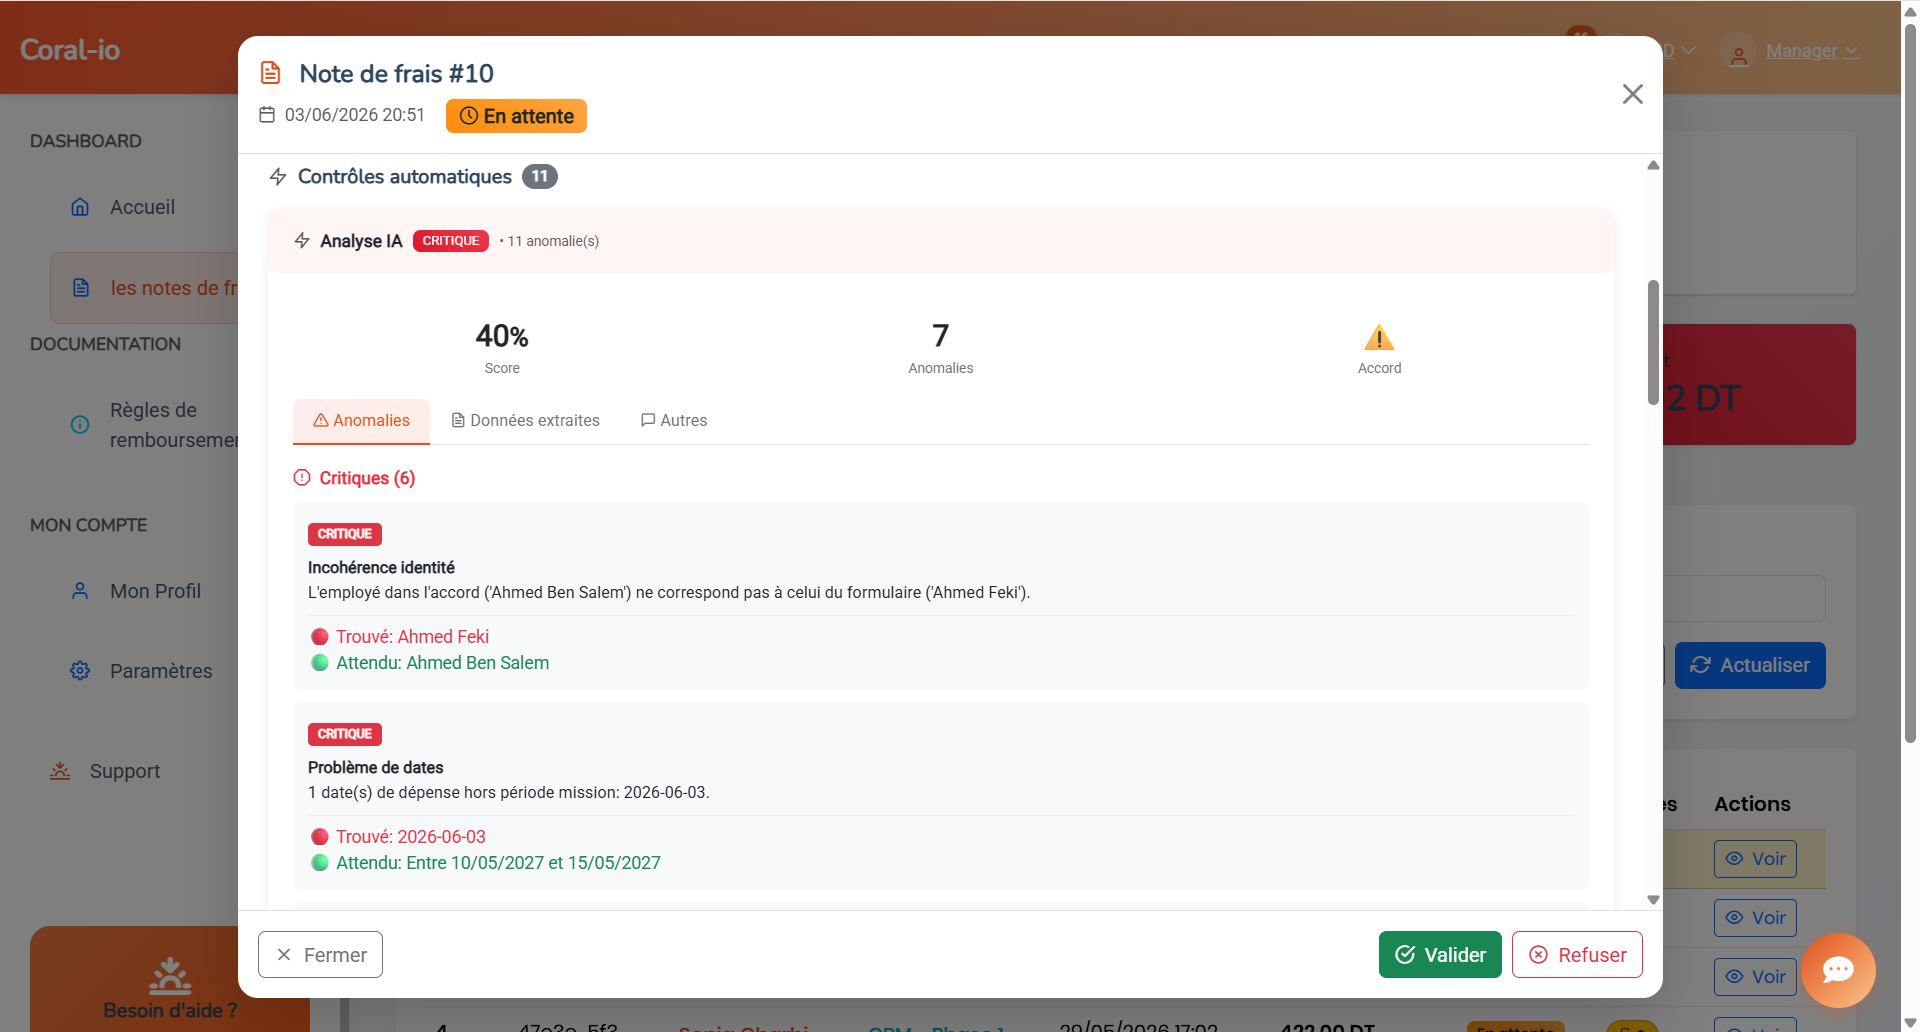
\includegraphics[width=\textwidth]{accord_analysis.png}
    \caption{Analyse IA de cohérence accord / note de frais}
    \label{fig:accord_analysis}
\end{figure}
\subparagraph{$\bullet$Validation de la facture (popup de détail)}
Lors de l'analyse d'une facture, le système utilise PaddleOCR pour extraire le texte du justificatif, puis un LLM (Gemma3:4b) détermine si celle-ci est valide. Le résultat est un booléen \texttt{is\_accurate} accompagné d'un score de confiance et d'une liste des anomalies détectées.

En cas de facture jugée non valide, une alerte s'affiche dans le popup de détail. L'utilisateur (manager ou administrateur) peut consulter le justificatif et décider de valider la note ou de la rejeter.

\begin{figure}[H]
    \centering
    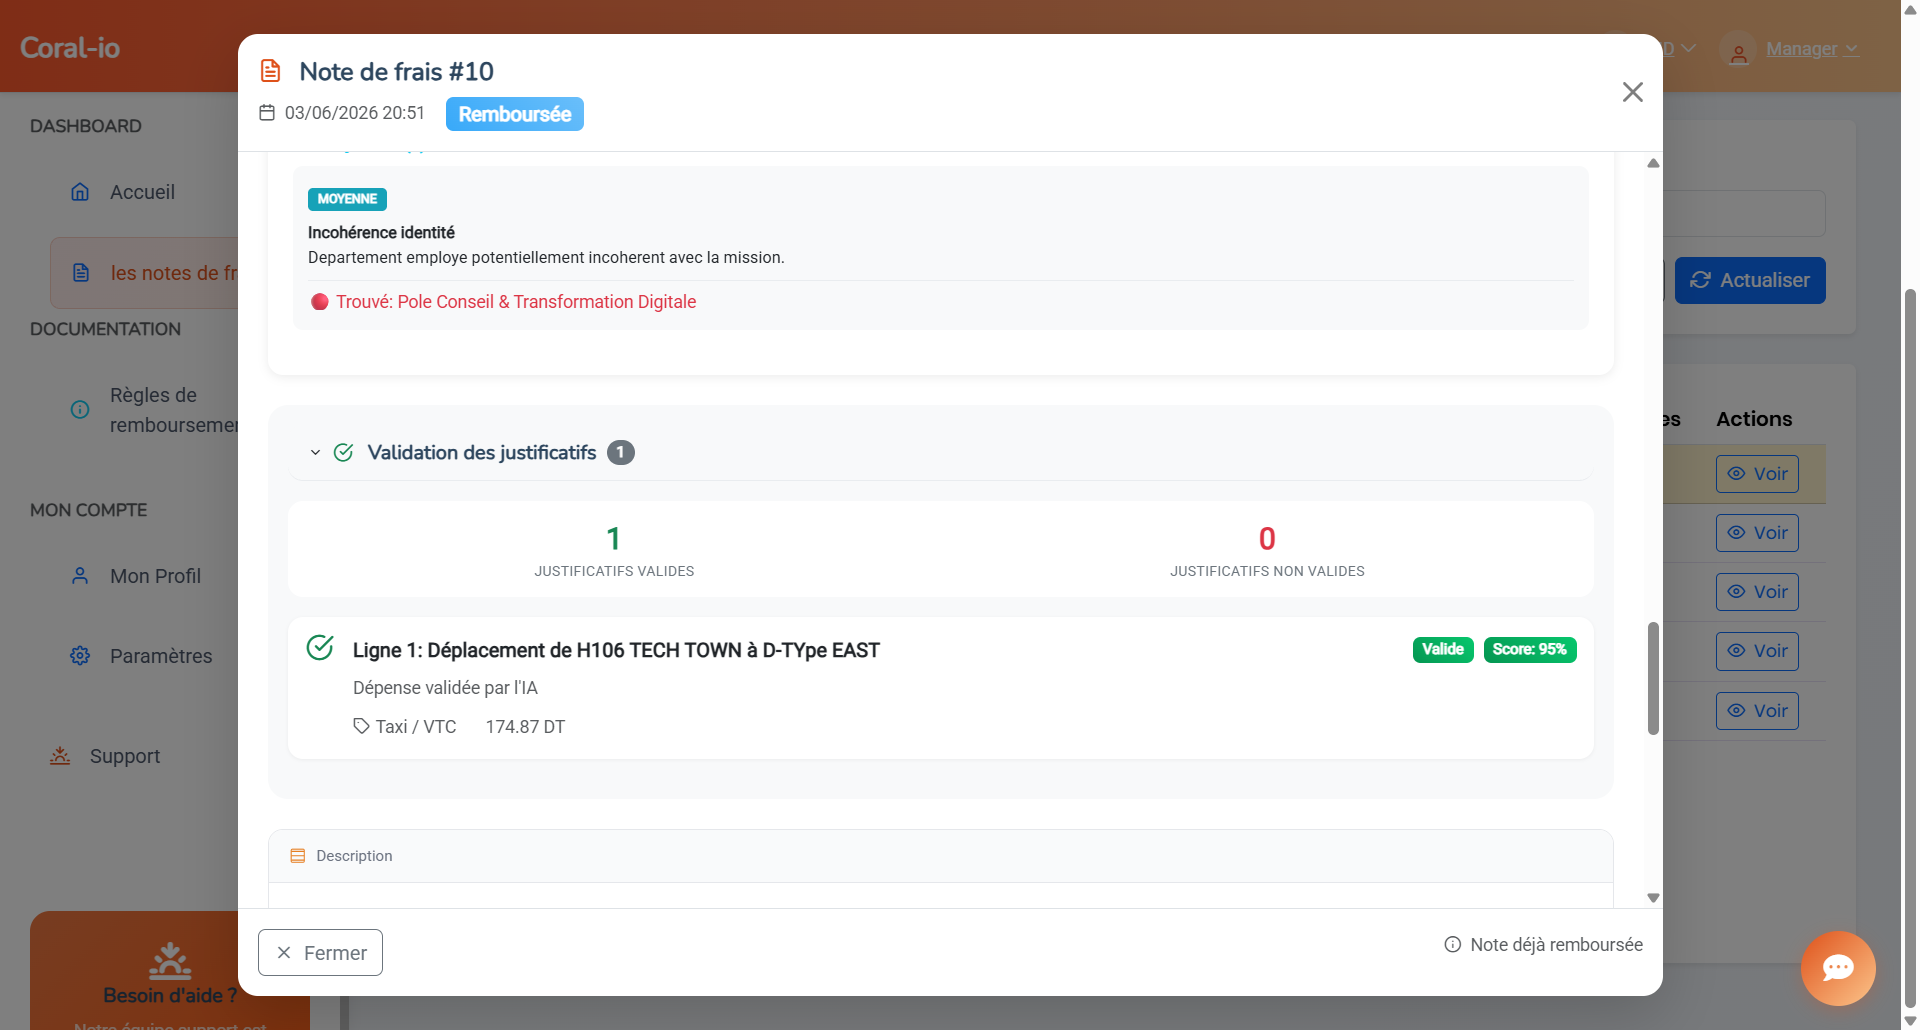
\includegraphics[width=\textwidth]{receipt_validation.png}
    \caption{Validation de la facture}
    \label{fig:receipt_validation}
\end{figure}
\subsubsection{Conclusion du déploiement}

La phase de déploiement a consisté à sauvegarder les modèles entraînés (FAISS, Isolation Forest) et à déployer l'architecture microservices. L'intégration dans l'interface web s'est traduite par la création d'une popup de détail (trois onglets : anomalies, données extraites, conclusion), de dashboards personnalisés (employé, manager, administrateur), d'un chatbot hybride et de notifications enrichies. L'objectif de ces démarches est de garantir une prise de décision optimale pour tous les acteurs.


\section{Chatbot hybride}



Un assistant conversationnel a été intégré dans les pages employé, manager et administrateur. Il repose sur une architecture hybride qui combine plusieurs moteurs pour offrir des réponses rapides et pertinentes.



\subsection{Modèle de langage utilisé}



Le chatbot intelligent utilise le modèle \textbf{Gemma3:4b} via le serveur \textbf{Ollama} (port 11434). Ce modèle de 4 milliards de paramètres a été choisi pour son équilibre entre performance et rapidité, avec un temps de réponse moyen de 450 ms par requête.



Les autres modèles testés (Mistral 7B et Llama 3 8B) ont été écartés car plus lents (respectivement 850 ms et 1200 ms) pour des résultats similaires.



\subsection{Architecture hybride}



Le chatbot combine trois moteurs :



\begin{itemize}

 \item Un \textbf{classificateur d'intention} (patterns regex) qui analyse la question et détermine sa complexité. La figure suivante montre un extrait du mécanisme de classification.

 

 \begin{figure}[H]

 \centering

 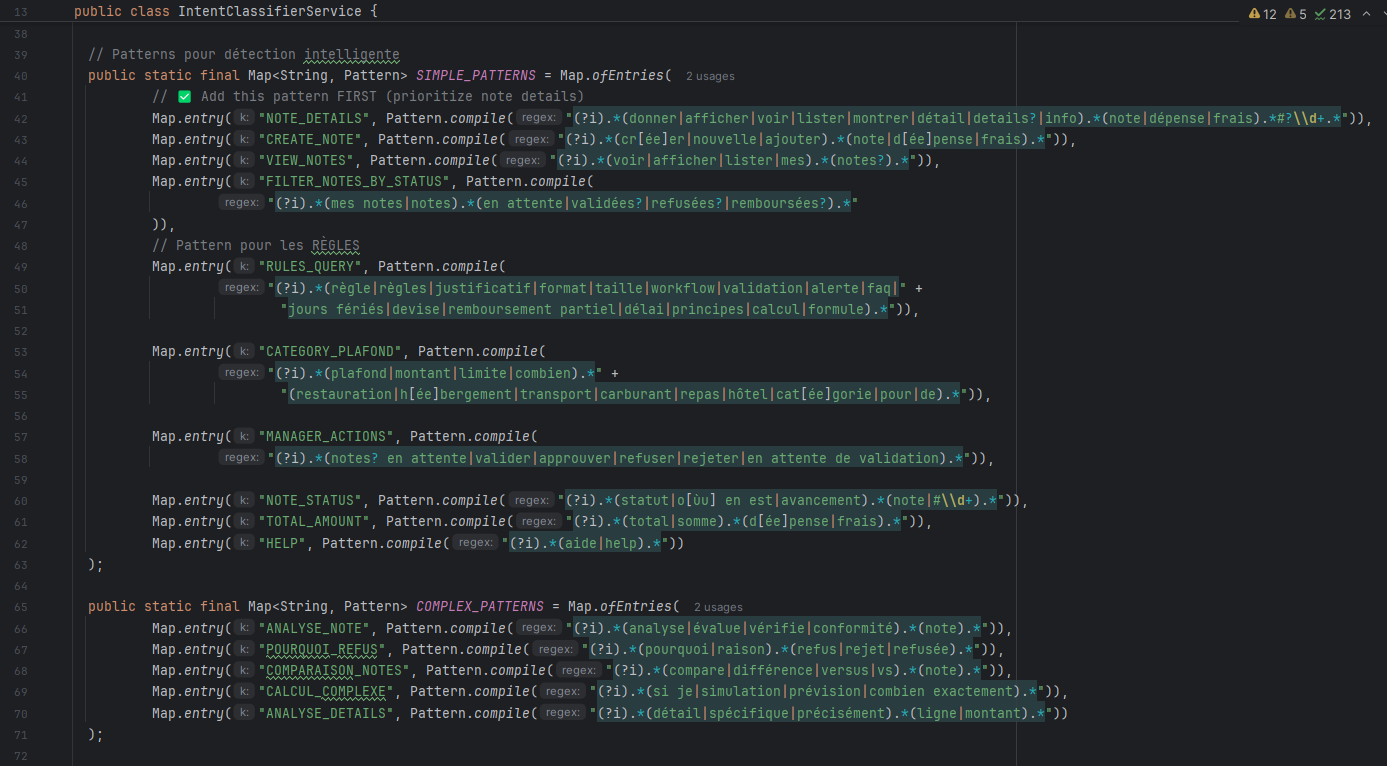
\includegraphics[width=1\textwidth]{chatbot/chatbot_patterns.png}

 \caption{Extrait des patterns de classification d'intention}

 \label{fig:chatbot_patterns}

 \end{figure}

 

 \item Un \textbf{chatbot simple} (réponses prédéfinies, règles métier, FAQ) pour les questions fréquentes (plafonds, workflow, justificatifs, etc.). Les réponses sont stockées en cache et dans un fichier JSON \texttt{rules-data.json}.



 \item Un \textbf{chatbot intelligent} basé sur LLM (Gemma3:4b) pour les questions complexes (analyse de note spécifique, comparaison de périodes, calculs de remboursement partiel).

\end{itemize}



\subsection{Structure du prompt pour le LLM}



Le prompt envoyé au modèle Gemma3:4b est construit dynamiquement. La figure suivante illustre la méthode de construction du prompt.



\begin{figure}[H]

 \centering

 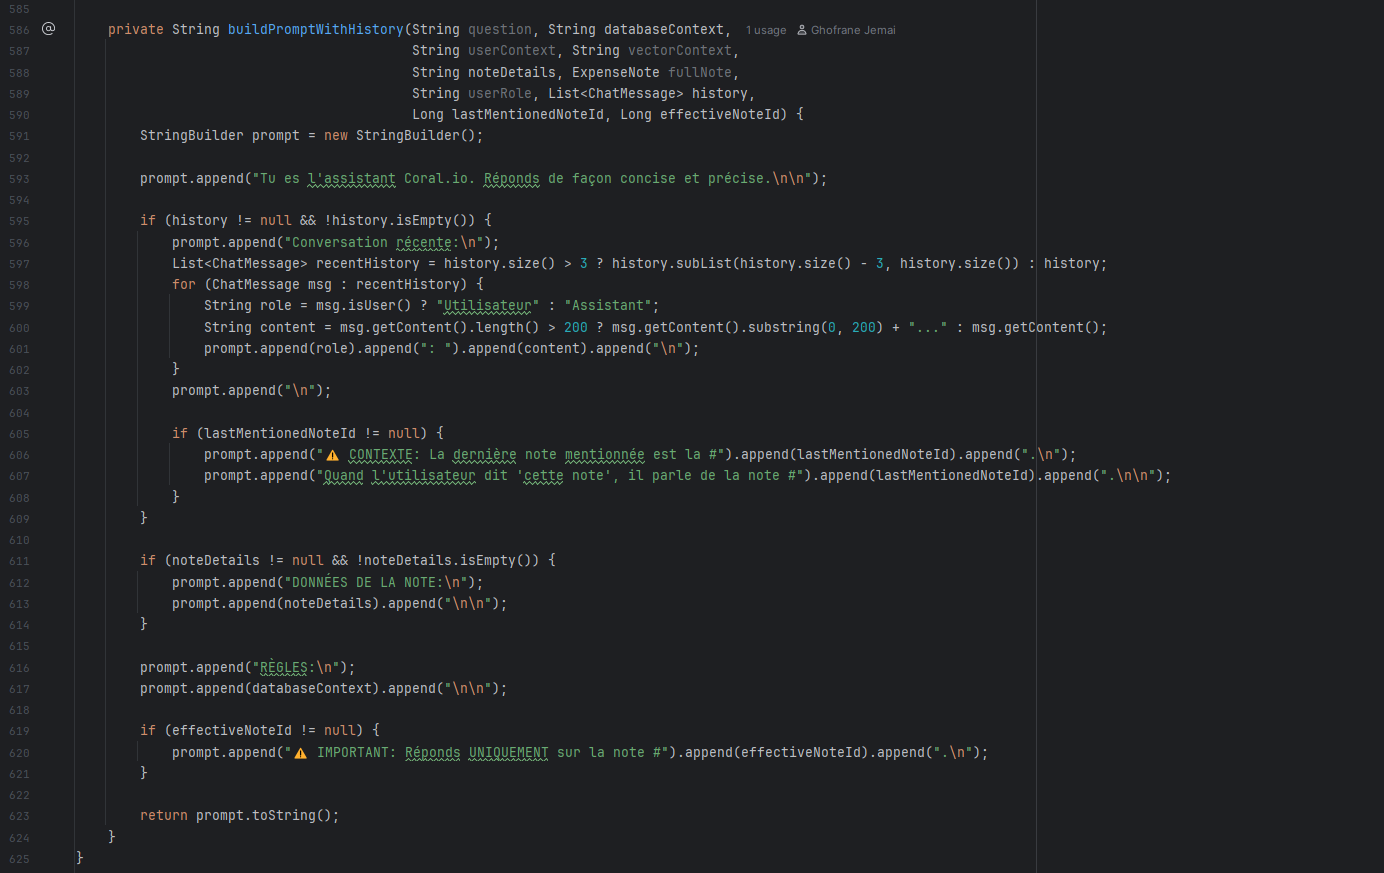
\includegraphics[width=1\textwidth]{chatbot/chatbot_prompt.png}

 \caption{Construction dynamique du prompt pour le LLM}

 \label{fig:chatbot_prompt}

\end{figure}



Le prompt inclut :

\begin{itemize}

 \item Le rôle de l'assistant

 \item Les données extraites de la note (via la base PostgreSQL)

 \item Les règles métier (plafonds, délais, justificatifs)

 \item Le contexte de session (historique des 3 derniers messages)

 \item La question de l'utilisateur

\end{itemize}



\subsection{Gestion du contexte de session}



Le chatbot maintient une session pour chaque utilisateur, stockée en base de données PostgreSQL avec :

\begin{itemize}

 \item Un token de session unique (UUID)

 \item L'historique des messages (user + bot)

 \item Le dernier ID de note mentionné (ex: \texttt{note \#92})

 \item La dernière question posée

 \item Une expiration automatique après 30 minutes d'inactivité

\end{itemize}



La figure ci-dessous montre un extrait du service de gestion de session.



\begin{figure}[H]

 \centering

 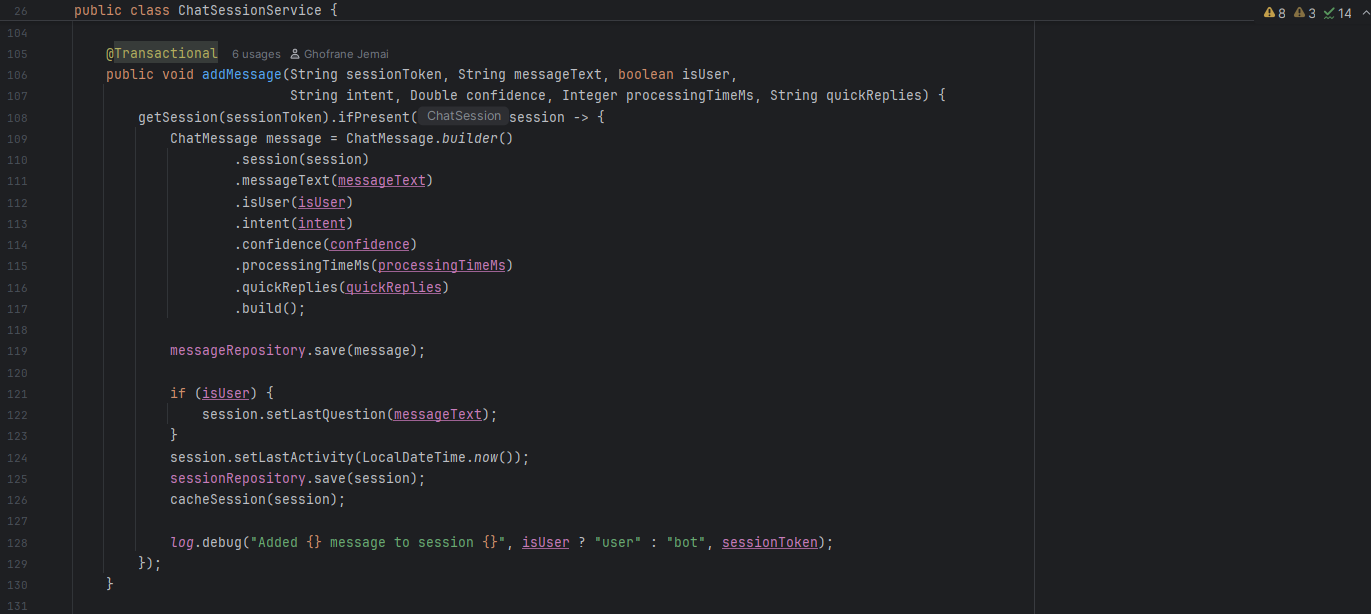
\includegraphics[width=1\textwidth]{chatbot/chatbot_session.png}

 \caption{Extrait du service de gestion de session}

 \label{fig:chatbot_session}

\end{figure}



\subsection{Routage des questions}



Le routage suit la logique illustrée dans la figure ci-après.



\begin{figure}[H]

 \centering

 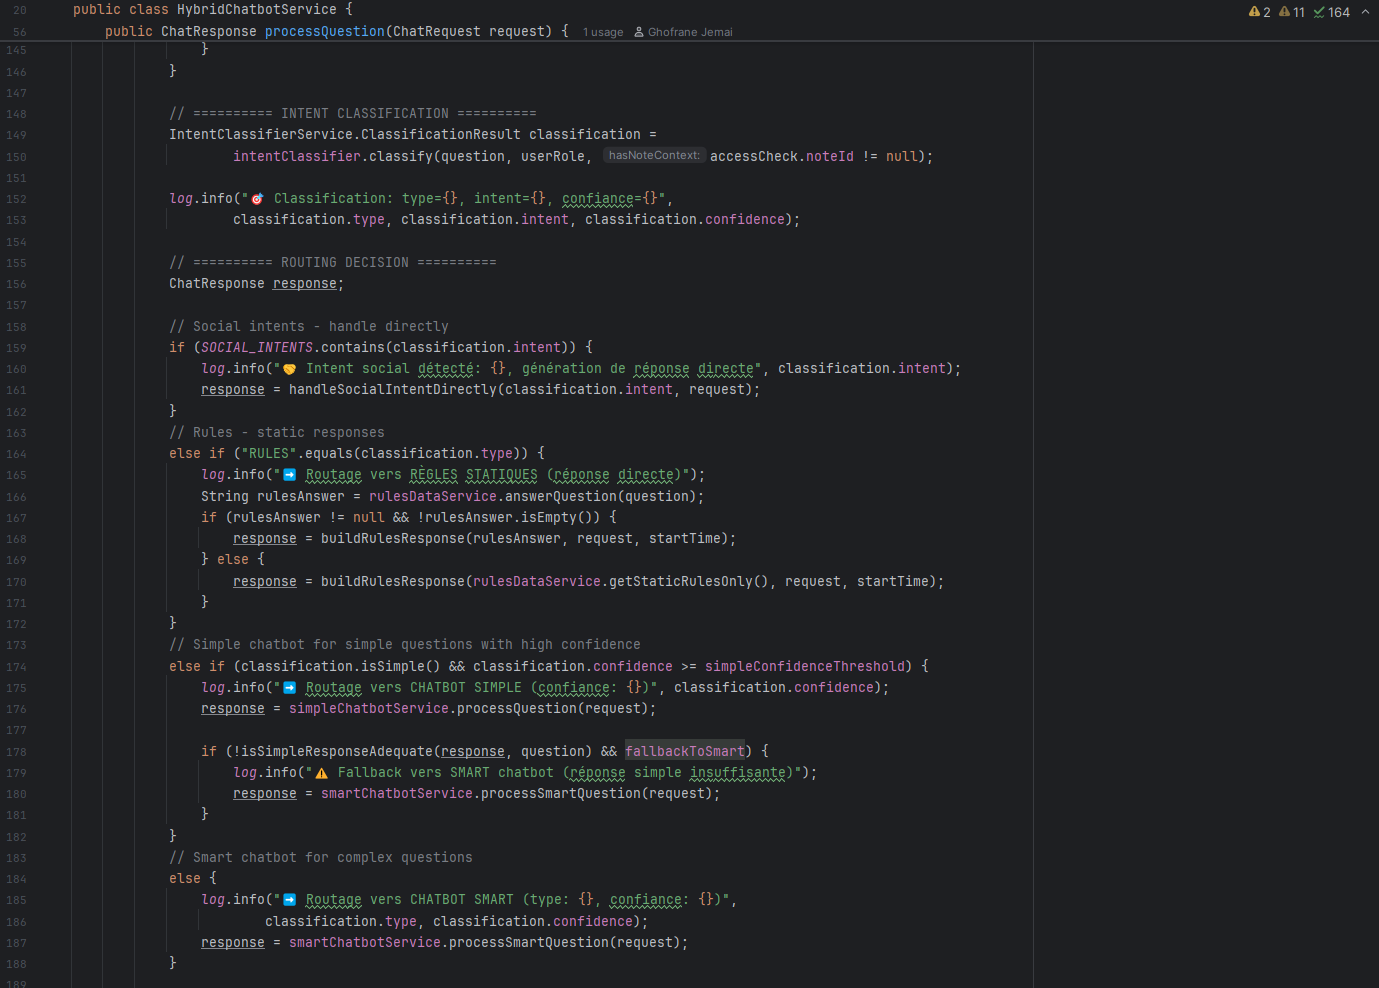
\includegraphics[width=1\textwidth]{chatbot/chatbot_routing.png}

 \caption{Logique de routage du chatbot hybride}

 \label{fig:chatbot_routing}

\end{figure}



\begin{enumerate}

 \item Les salutations, remerciements et au revoir → réponse directe sans LLM

 \item Les questions sur les règles statiques → réponse depuis le cache JSON

 \item Les questions simples (confiance > 60\%) → chatbot simple

 \item Les questions complexes (analyse de note, comparaison, calcul) → LLM Gemma3:4b

\end{enumerate}



La figure suivante illustre le flux de traitement d'une question par le chatbot hybride.



\begin{figure}[H]

 \centering

 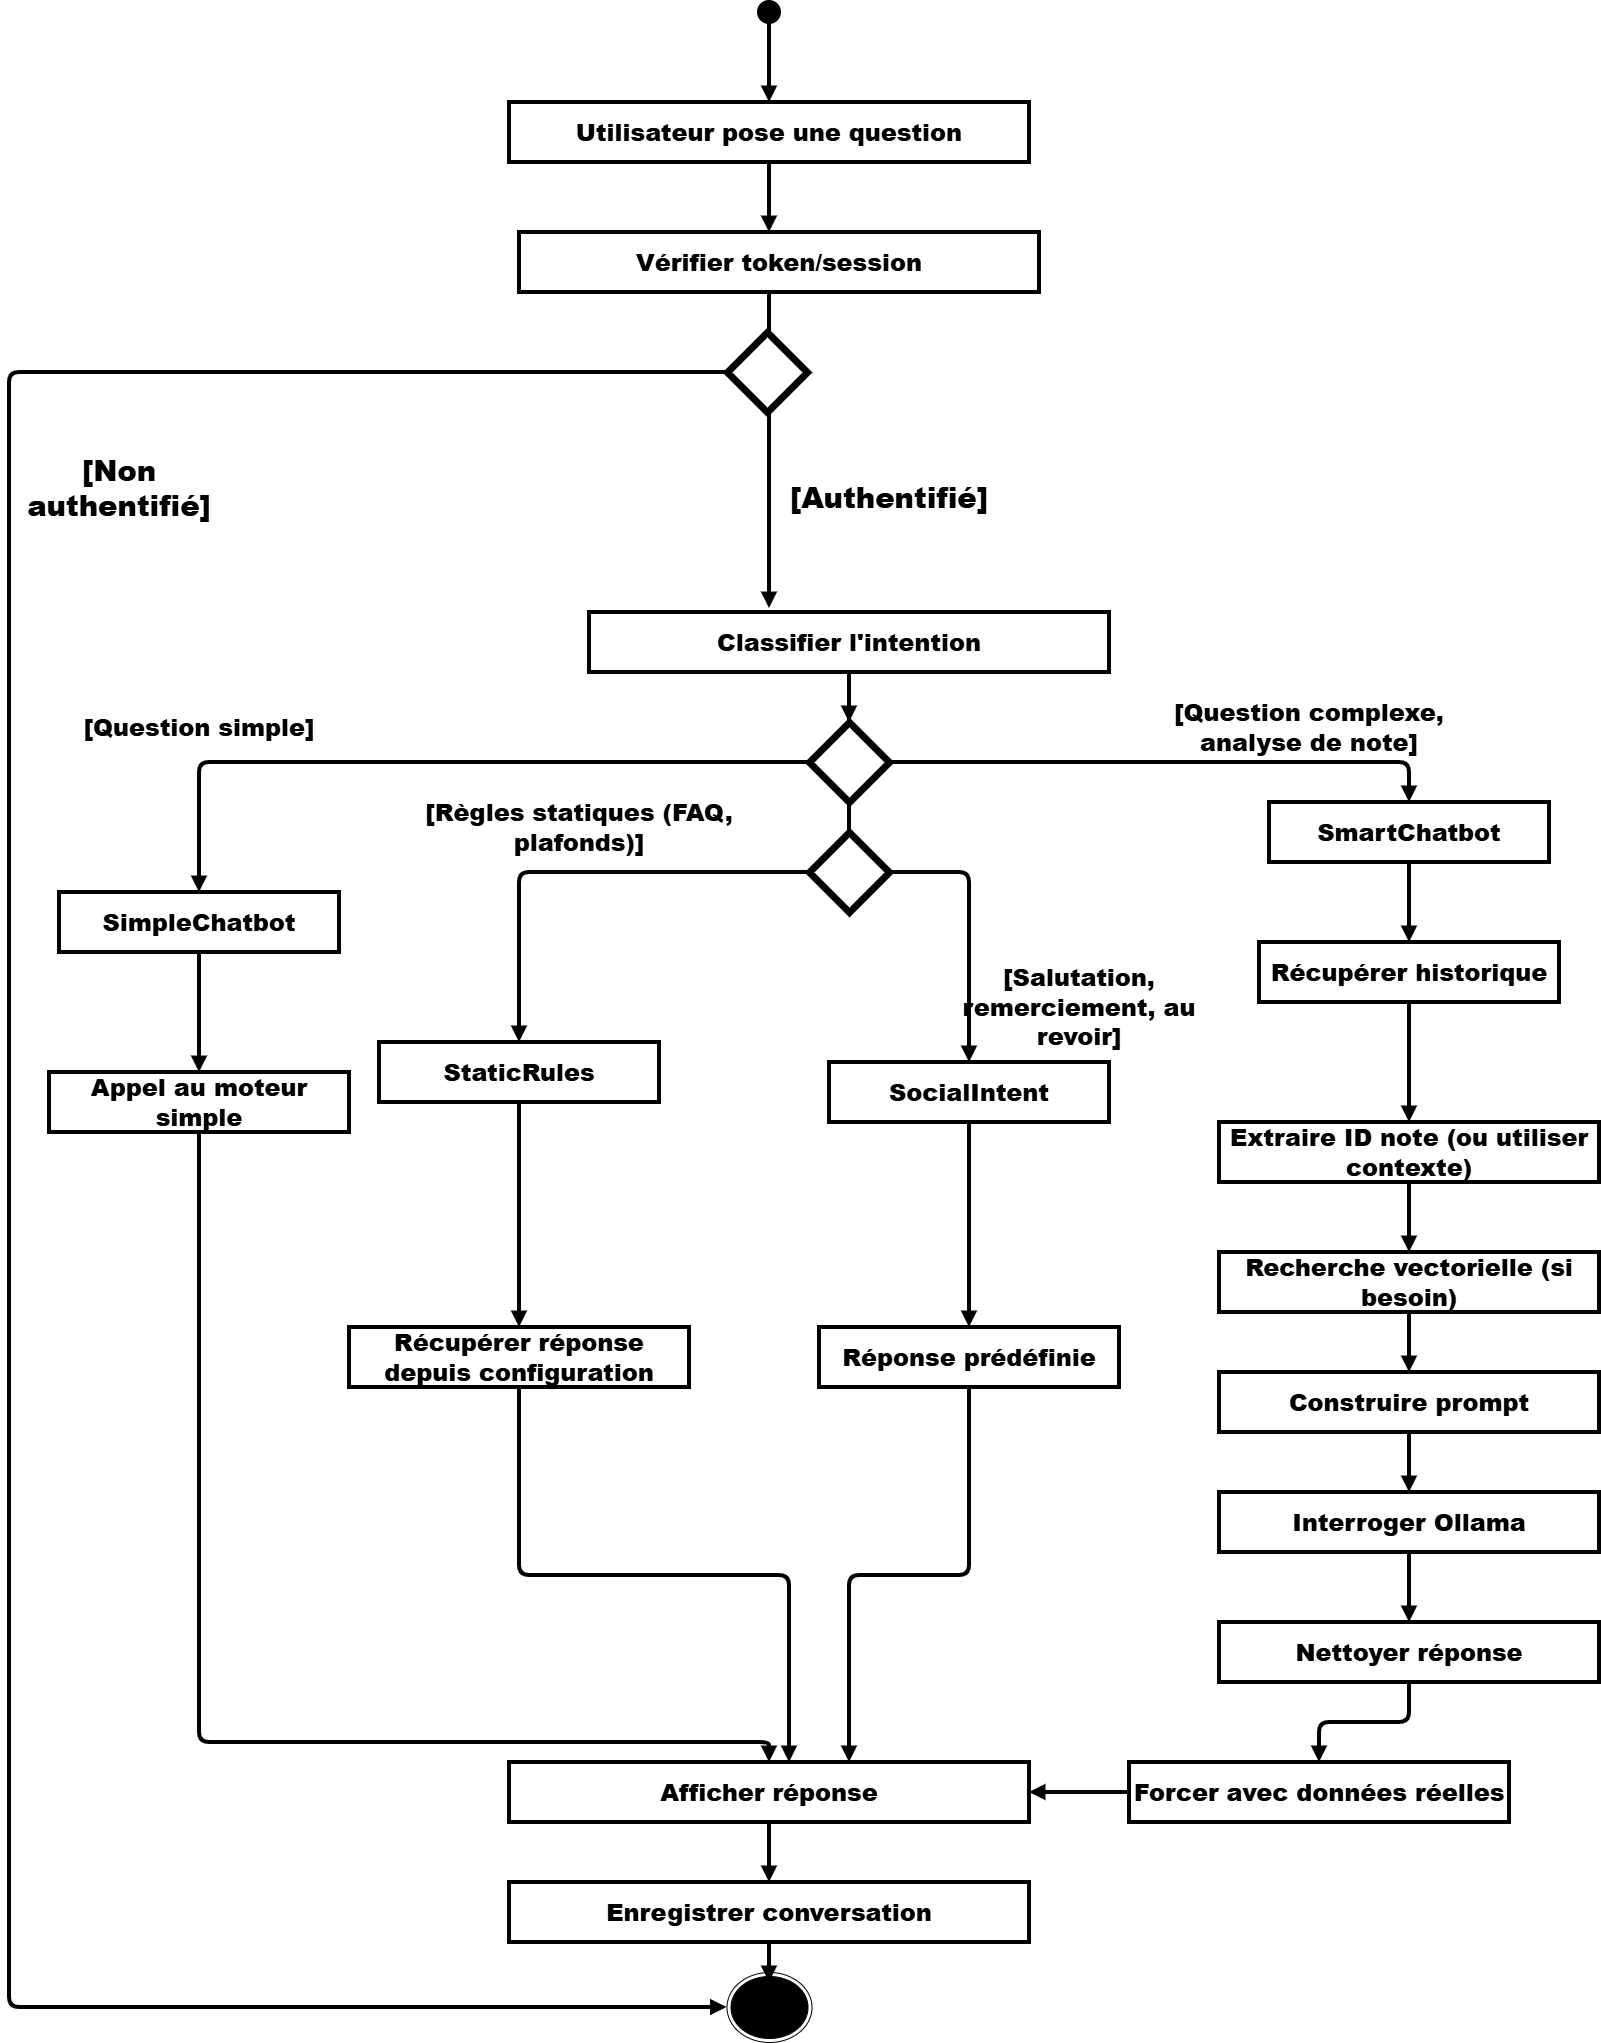
\includegraphics[width=0.9\textwidth,height=0.8\textheight]{chatbot.png}

 \caption{Diagramme d'activité du chatbot hybride}

 \label{fig:chatbot_activity}

\end{figure}

\newpage

Le chatbot est accessible via une icône flottante en bas à droite et peut fournir des réponses en temps réel, des liens vers les pages appropriées, et des « quick replies » pour guider l'utilisateur.



\begin{figure}[H]

 \centering

 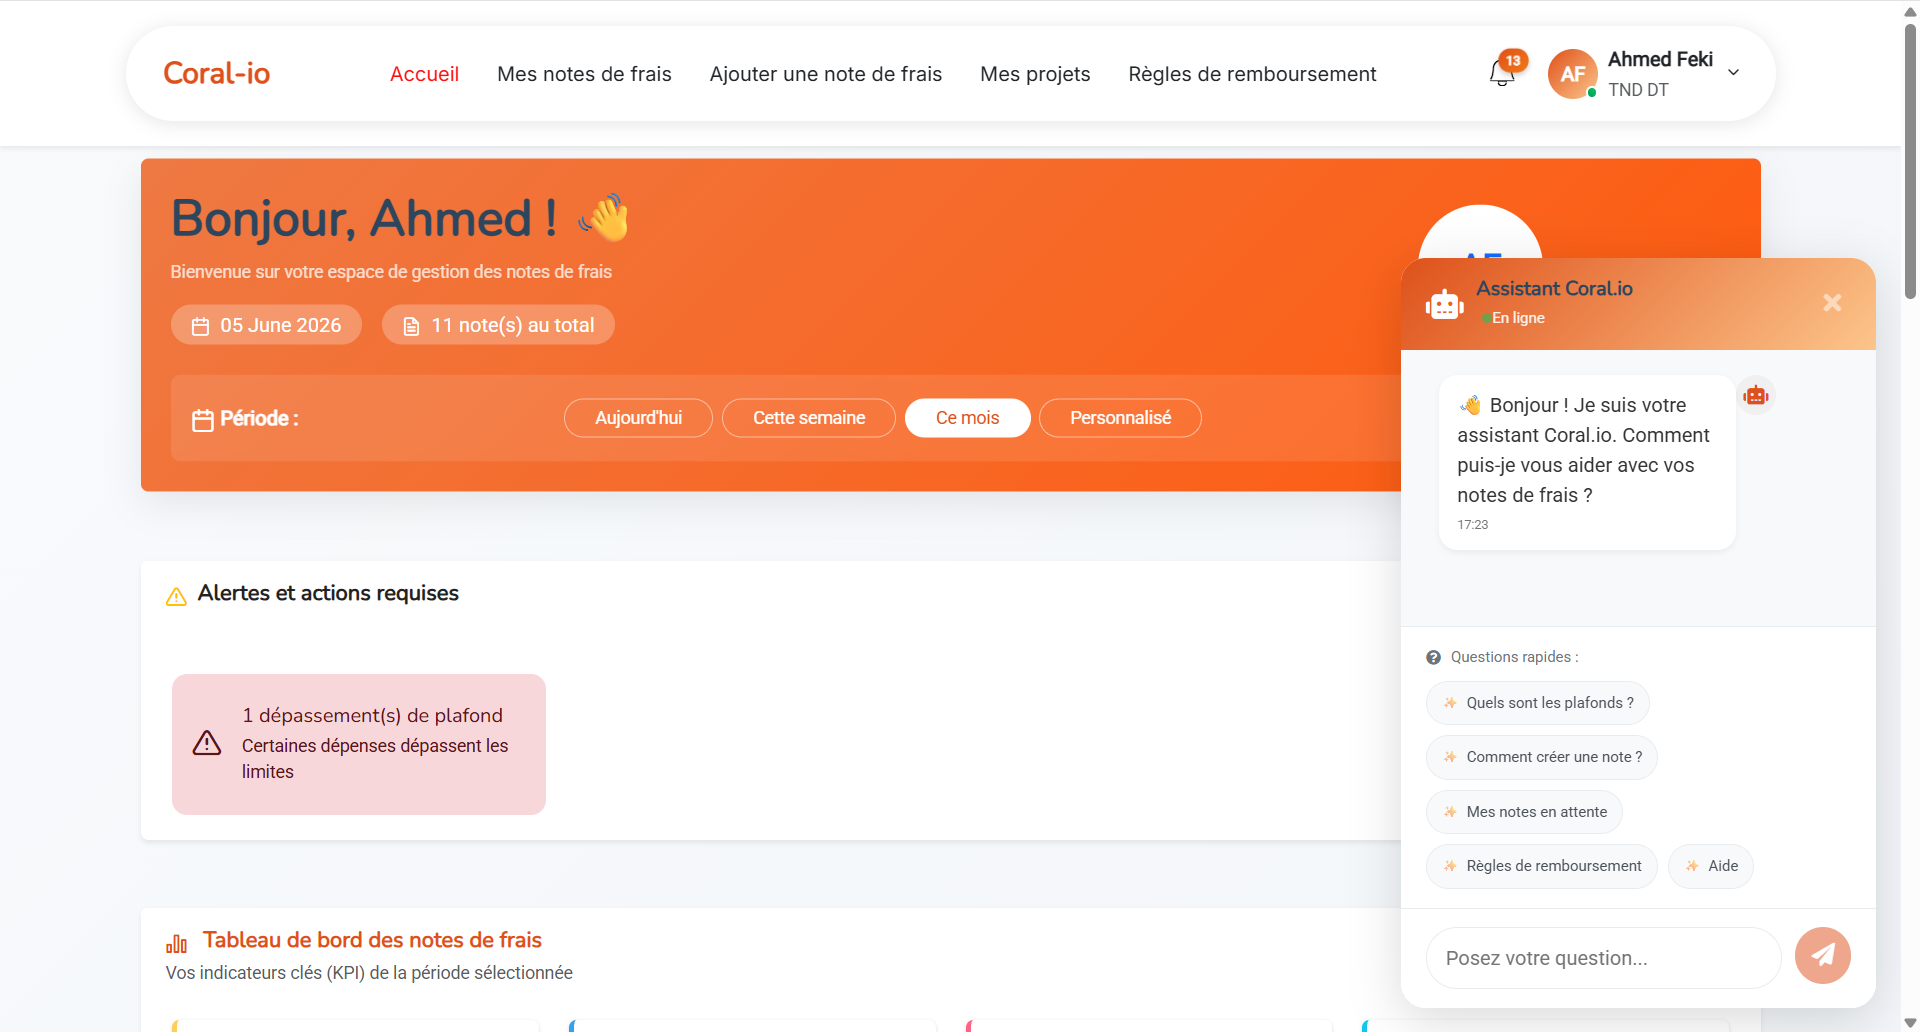
\includegraphics[width=\textwidth]{chatbot_interface.png}

 \caption{Interface du chatbot hybride intégré}

 \label{fig:chatbot_interface}

\end{figure}



\section{Tableaux de bord}

En parallèle des modèles de détection, nous avons développé trois tableaux de bord interactifs (employé, manager, administrateur).



\subsection{Tableau de bord employé}

Ce dashboard, accessible depuis la page d'accueil de l'employé, présente :

\begin{itemize}

 \item Des cartes KPI : notes en attente, approuvées, refusées, remboursées.

 \item Deux graphiques linéaires : évolution du nombre de notes et évolution des montants (avec filtres temporels : aujourd'hui, semaine, mois, personnalisé).

 \item Un diagramme en camembert de répartition des statuts.

 \item Un graphique à barres des dépenses par catégorie (top catégories).

 \item Des alertes personnelles : notes bloquées (en attente >7 jours), dépassements de plafond, notes refusées récentes.

\end{itemize}



\begin{figure}[H]

\centering

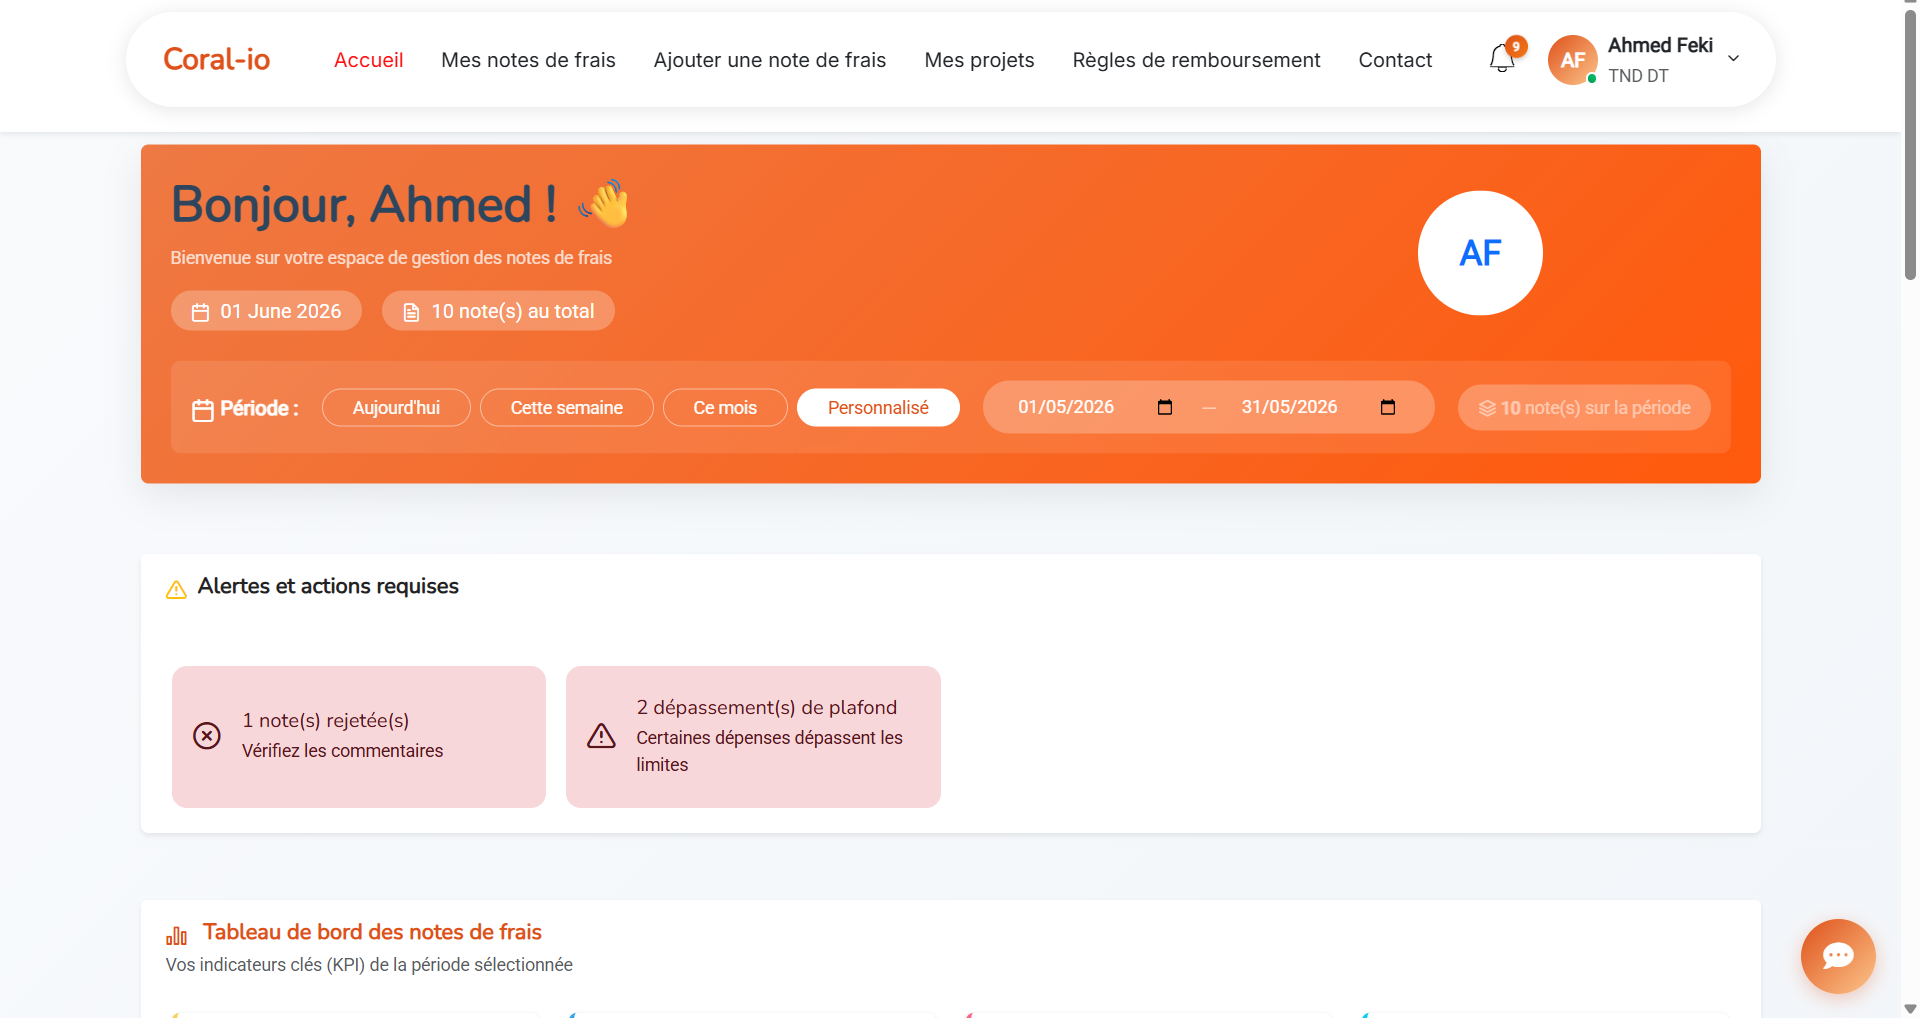
\includegraphics[width=\textwidth]{dashboard-emp/Suite_1.png}

\caption{Tableau de bord employé}

\label{fig:employee_dashboard}

\end{figure}

\begin{figure}[H]

\centering

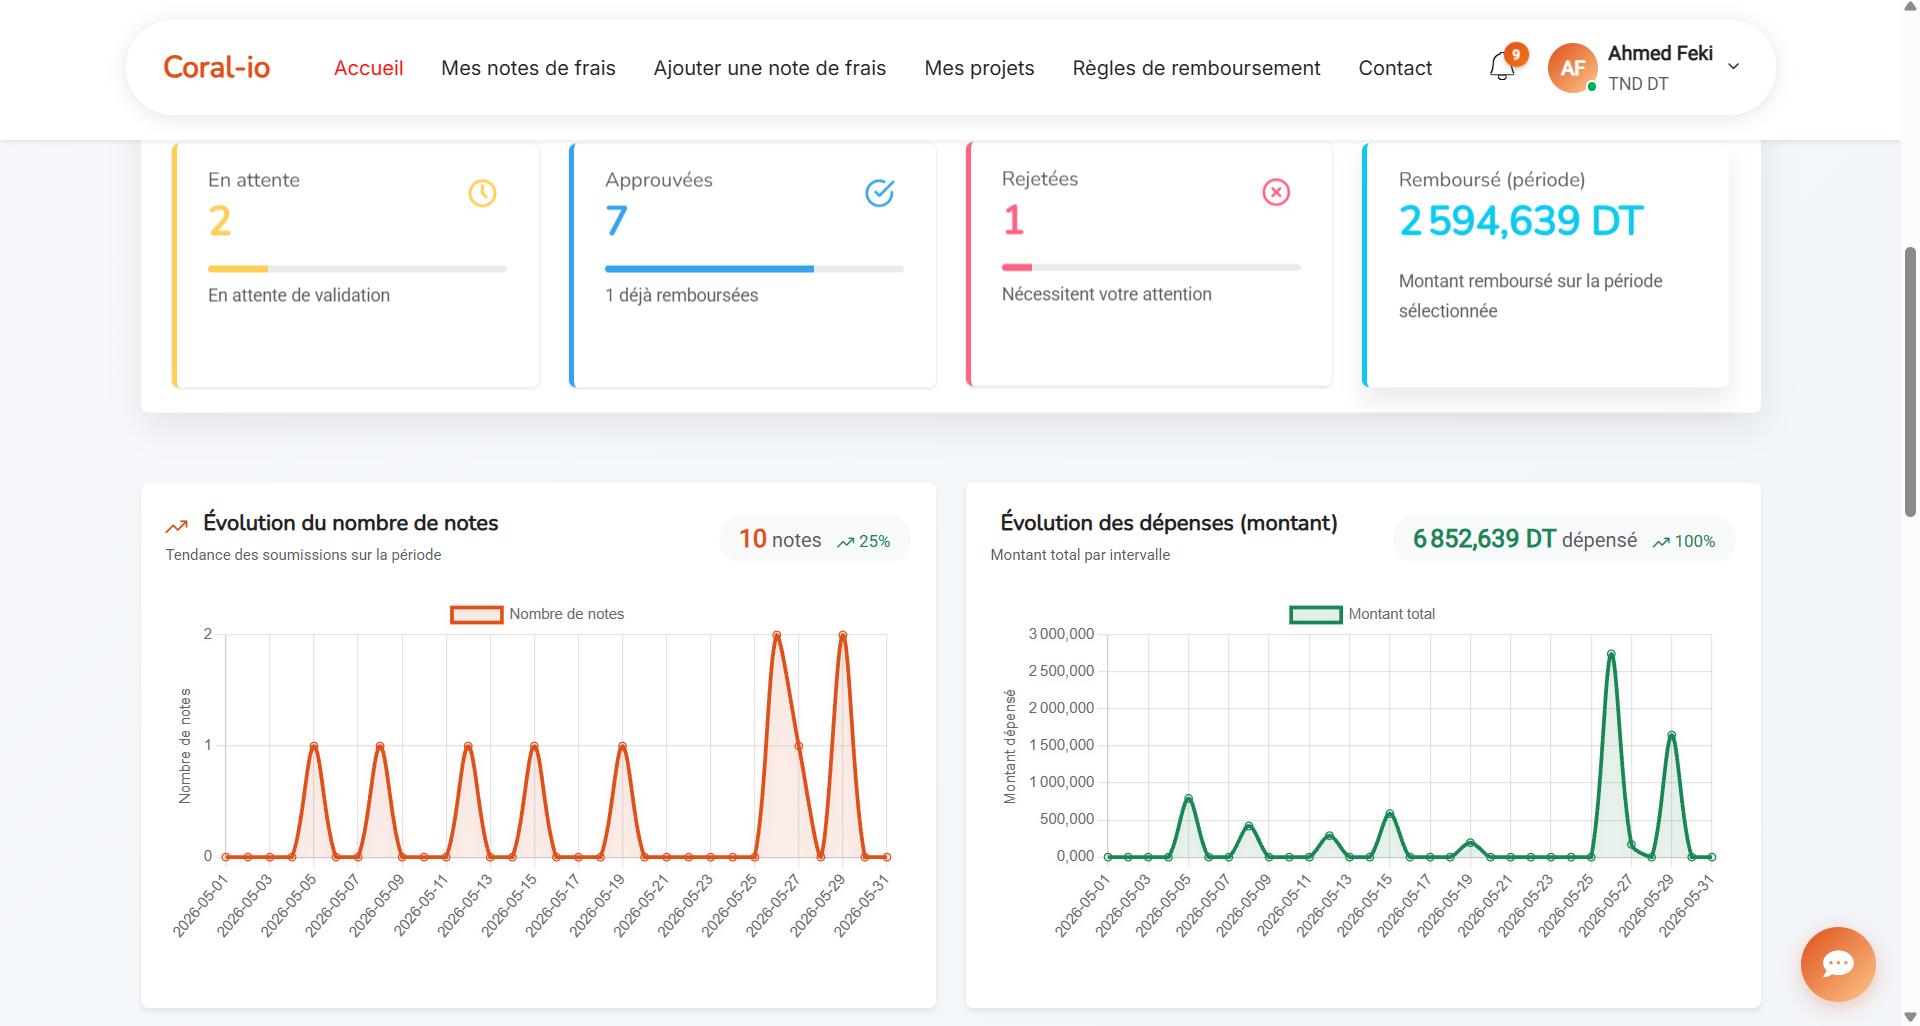
\includegraphics[width=\textwidth]{dashboard-emp/Suite_2.png}

\caption{Suite 1 du tableau de bord employé}

\label{fig:employee_dashboard}

\end{figure}

\begin{figure}[H]

\centering

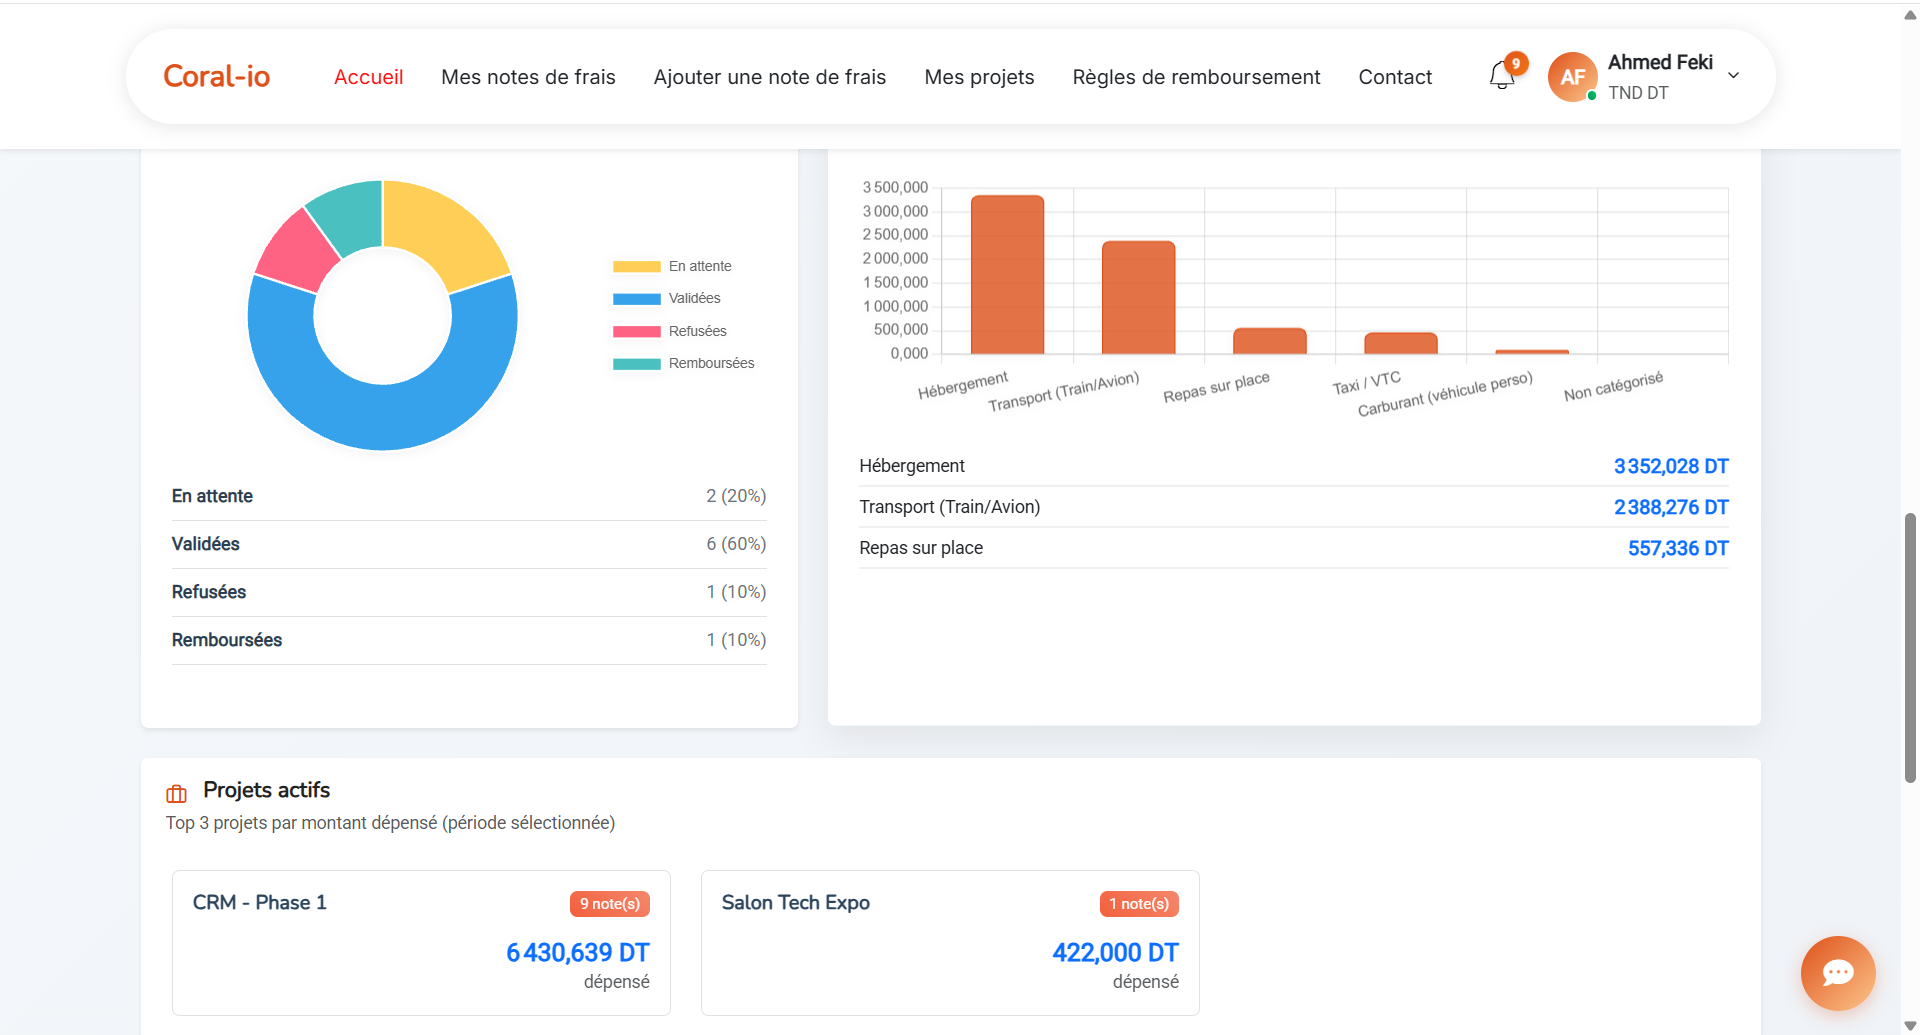
\includegraphics[width=\textwidth]{dashboard-emp/Suite_3.png}

\caption{Suite 2 du tableau de bord employé}

\label{fig:employee_dashboard}

\end{figure}

\begin{figure}[H]

\centering

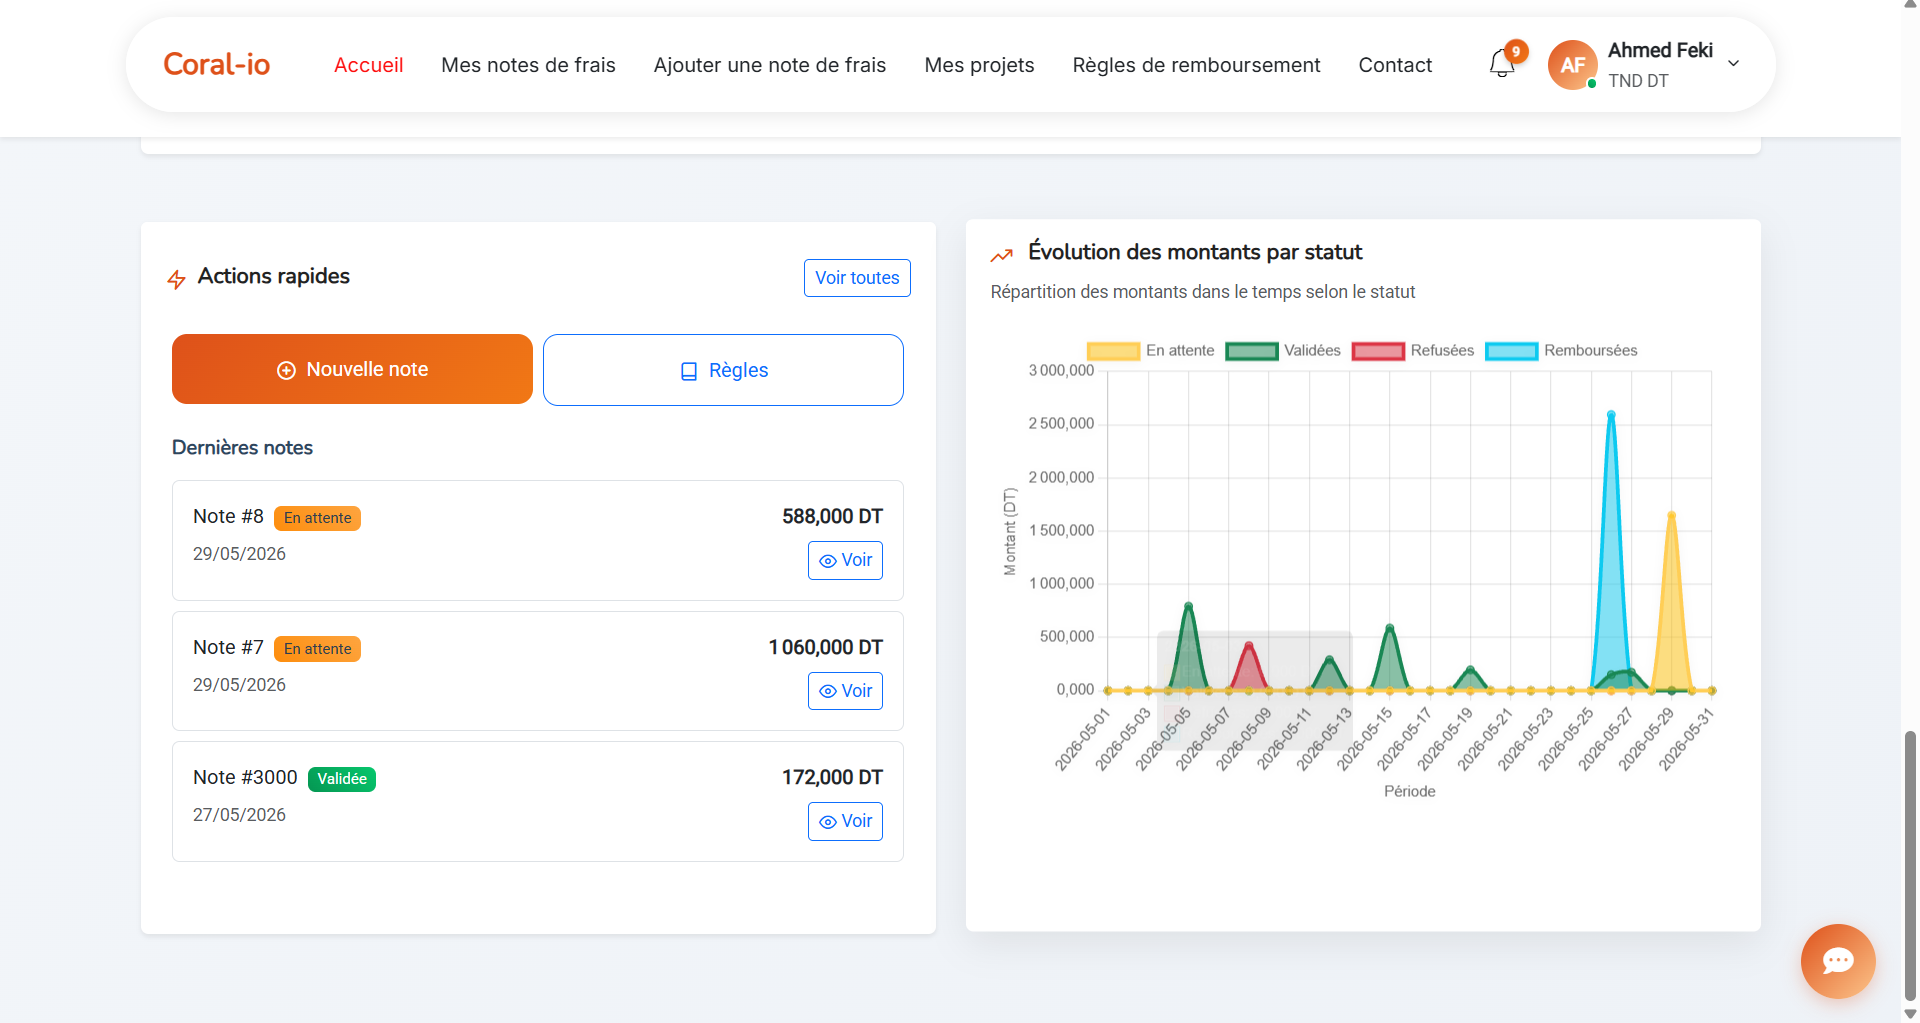
\includegraphics[width=\textwidth]{dashboard-emp/Suite_4.png}

\caption{Suite 3 du tableau de bord employé}

\label{fig:employee_dashboard}

\end{figure}



\subsection{Tableau de bord manager}

Le manager dispose d'une vue synthétique sur son département :

\begin{itemize}

 \item KPIs : notes en attente dans le département, montant total en attente, délai moyen de traitement.

 \item Graphique d'évolution des soumissions sur les 7 derniers jours.

 \item Top 5 des dépensiers (montant total remboursé) et top 5 des employés les plus actifs (nombre de notes).

 \item Répartition des statuts (camembert).

 \item Dépenses par catégorie : tableau détaillé (nombre, montant, moyenne) et graphique à barres.

 \item Section « Alertes \& anomalies » listant les notes avec anomalies IA, doublons, dépassements de budget.

 \item Filtres temporels et par statut.

\end{itemize}



\begin{figure}[H]

\centering

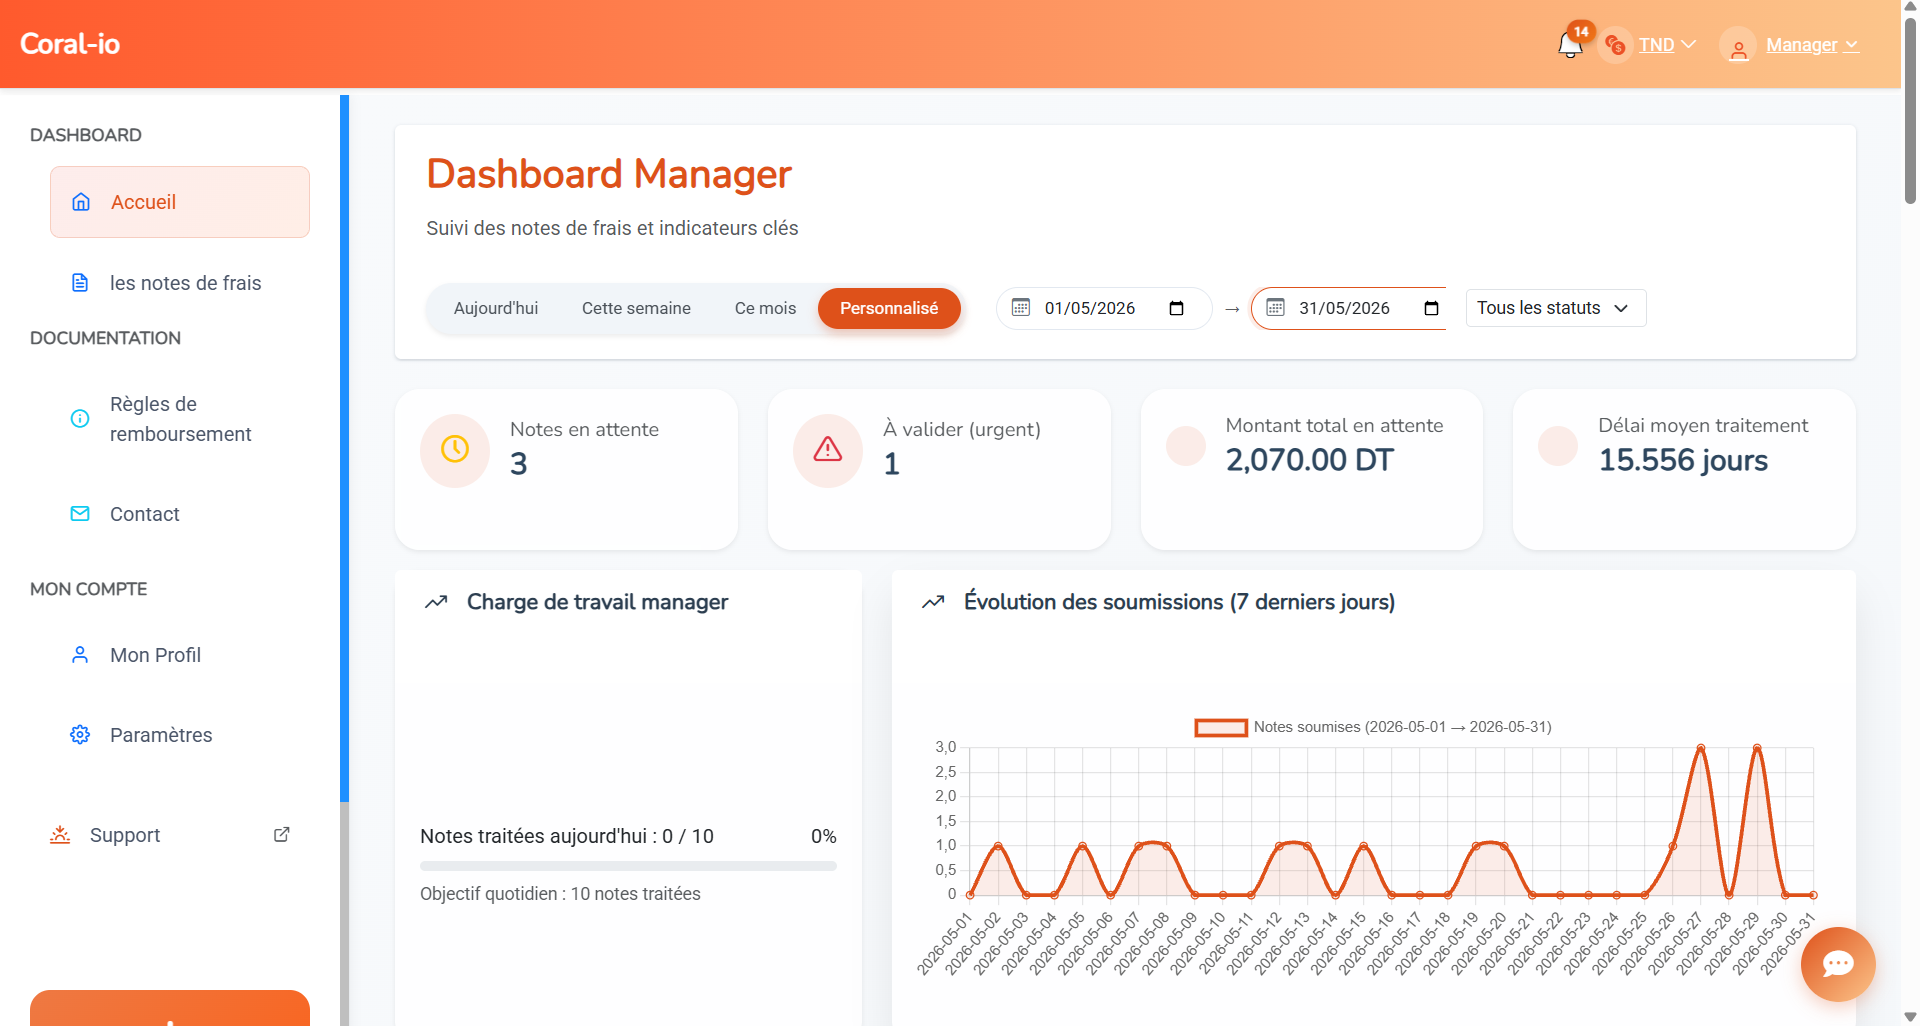
\includegraphics[width=\textwidth]{dashboard-manager/Suite_1.png}

\caption{Tableau de bord manager}

\label{fig:manager_dashboard}

\end{figure}

\begin{figure}[H]

\centering

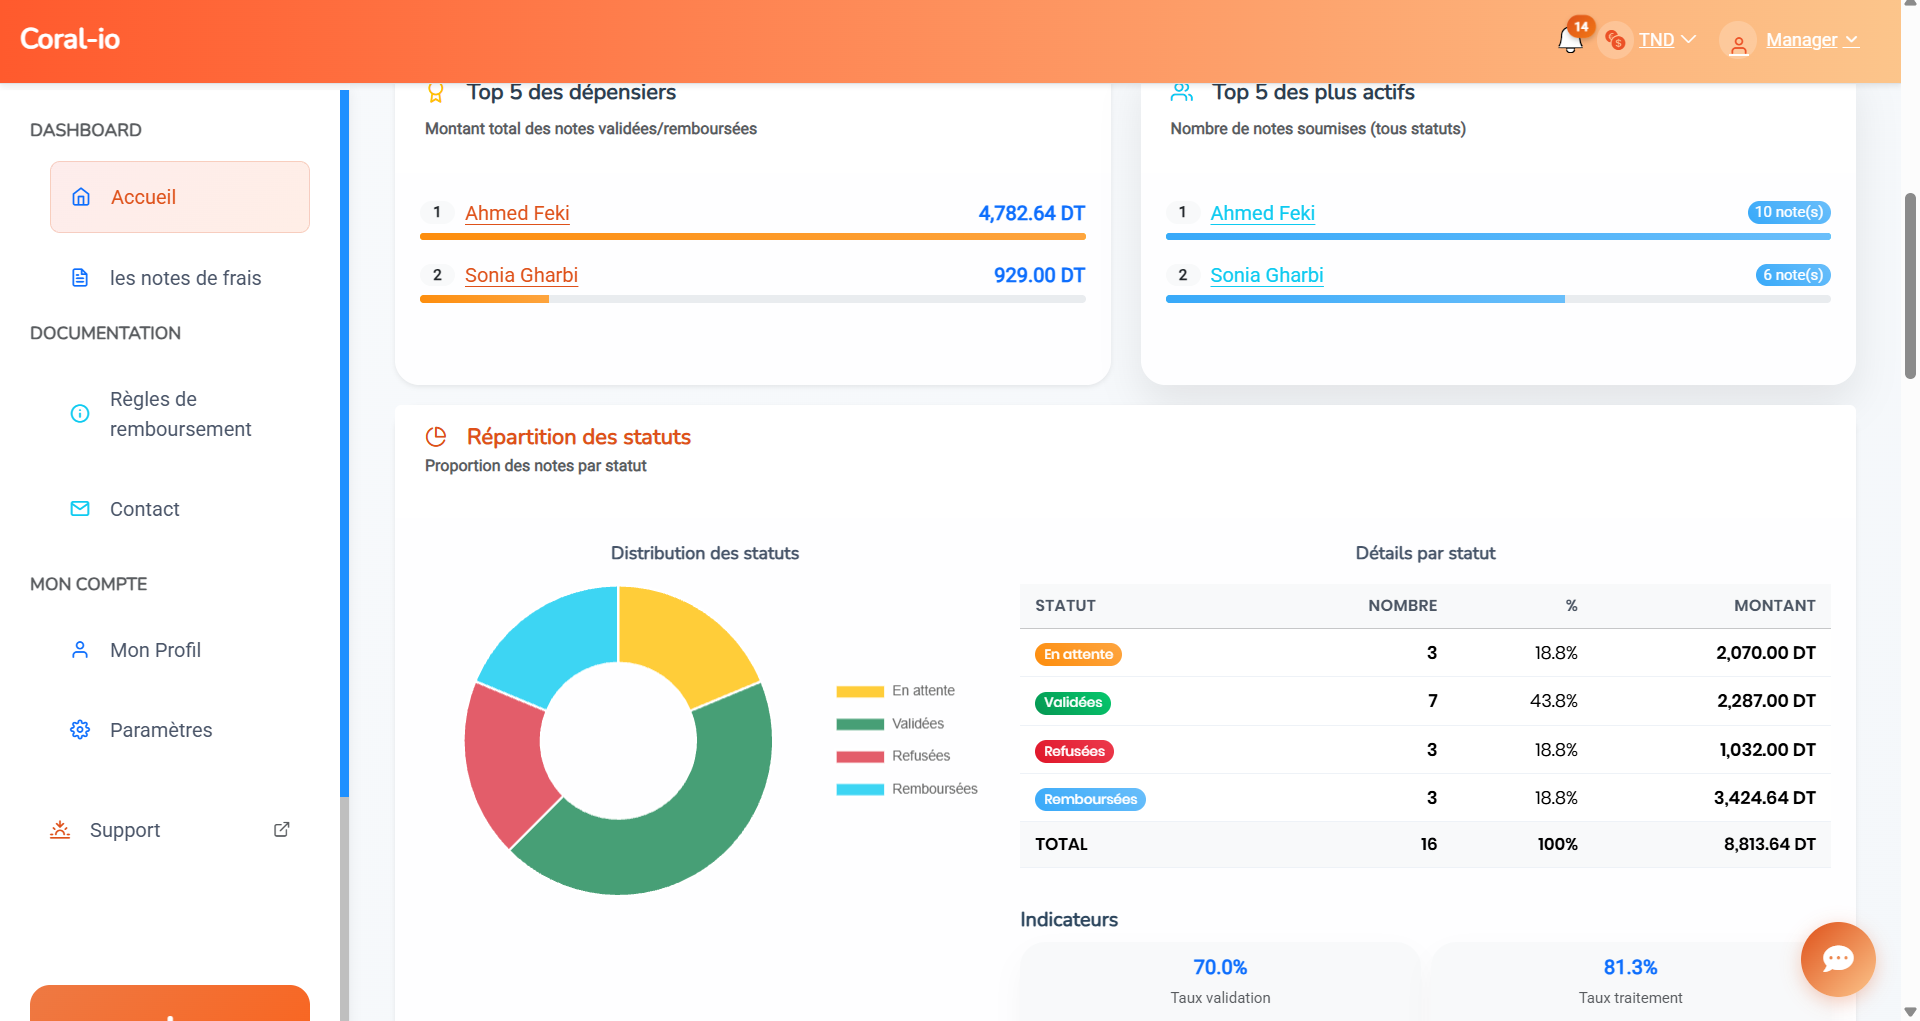
\includegraphics[width=\textwidth]{dashboard-manager/Suite_2.png}

\caption{Suite 1 du tableau de bord manager}

\label{fig:manager_dashboard}

\end{figure}

\begin{figure}[H]

\centering

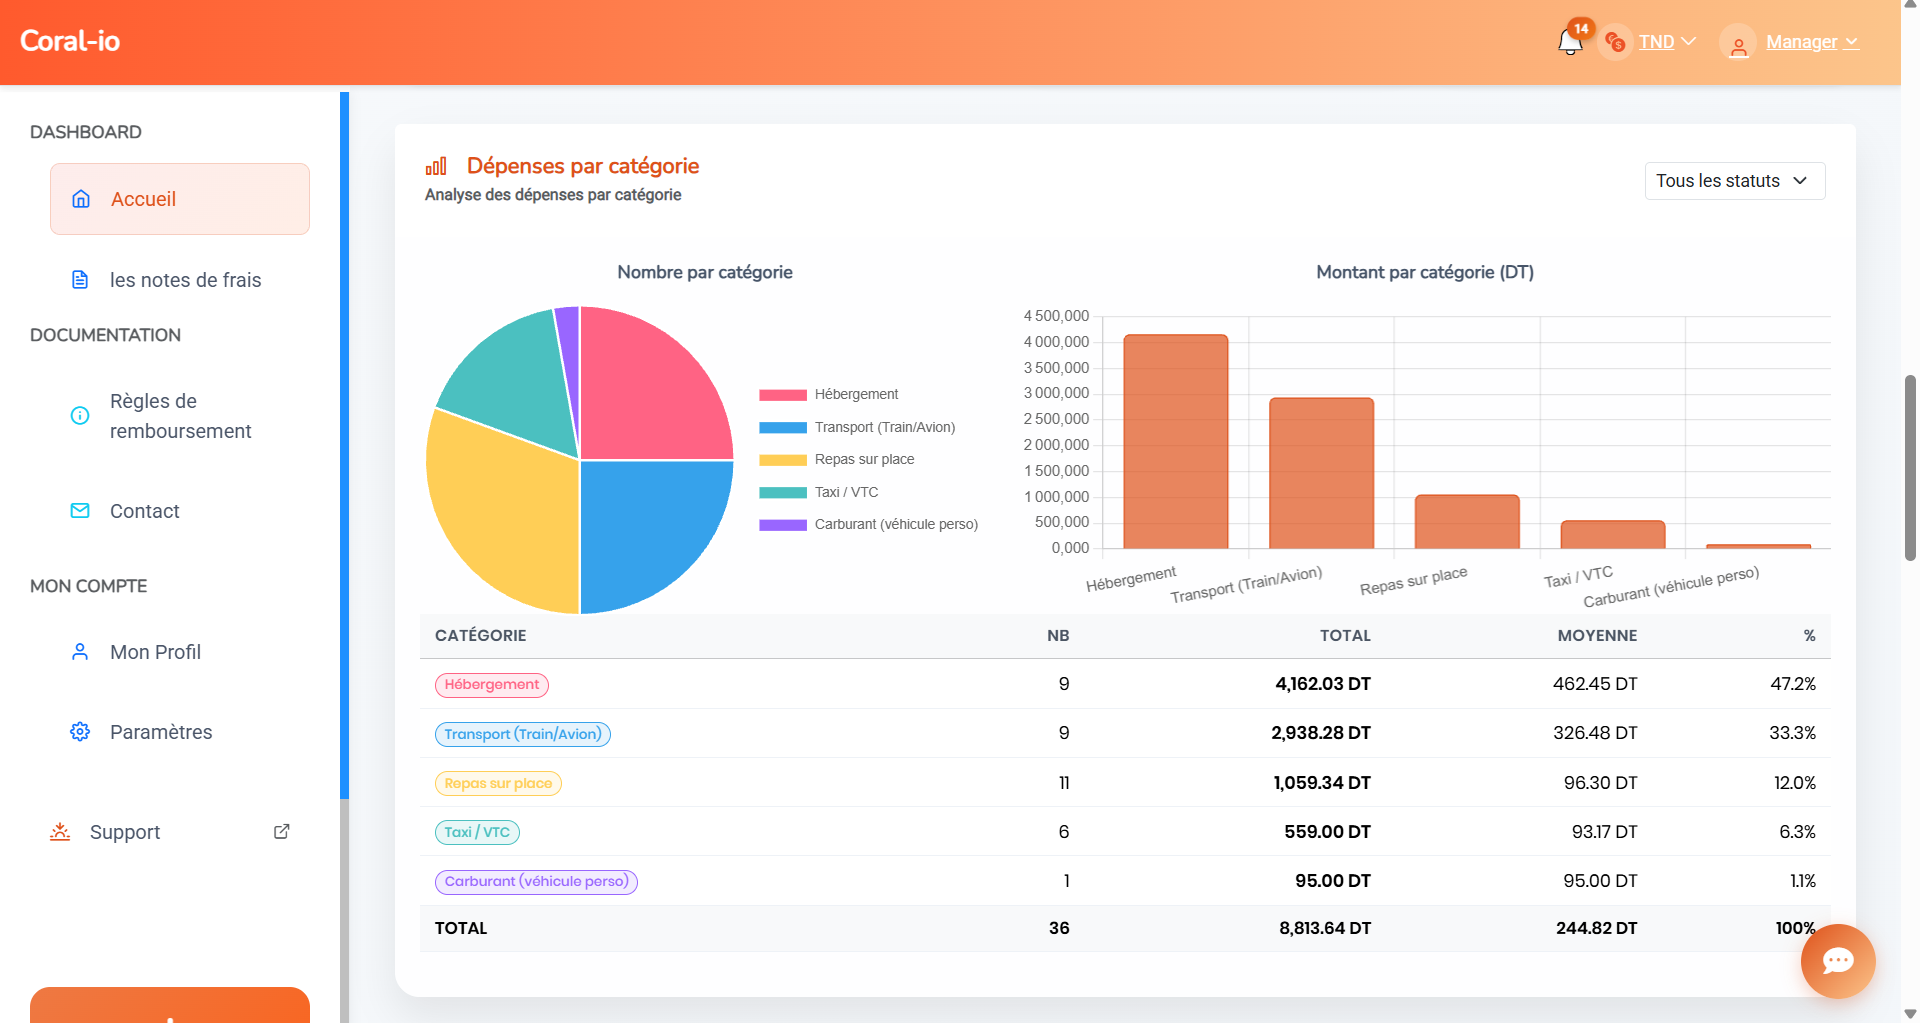
\includegraphics[width=\textwidth]{dashboard-manager/Suite_3.png}

\caption{Suite 2 du tableau de bord manager}

\label{fig:manager_dashboard}

\end{figure}

\begin{figure}[H]

\centering

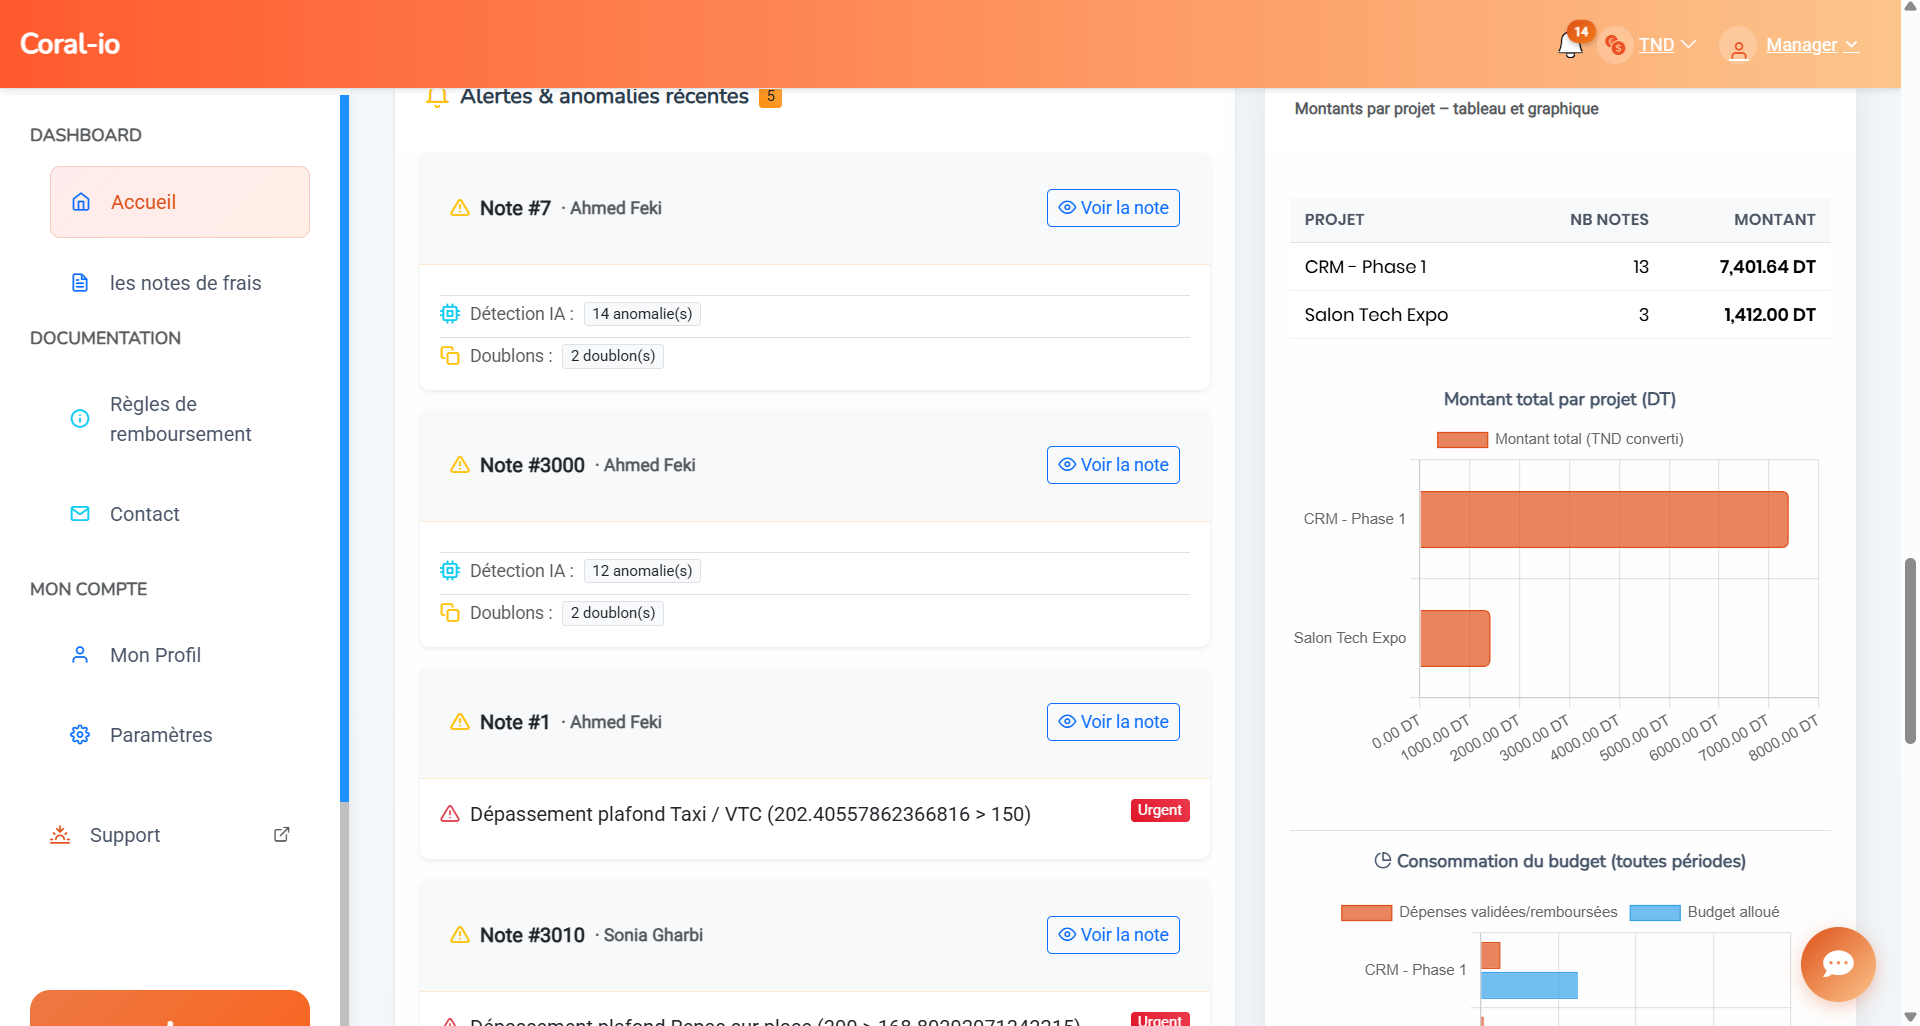
\includegraphics[width=\textwidth]{dashboard-manager/Suite_4.png}

\caption{Suite 3 du tableau de bord manager}

\label{fig:manager_dashboard}

\end{figure}

\begin{figure}[H]

\centering

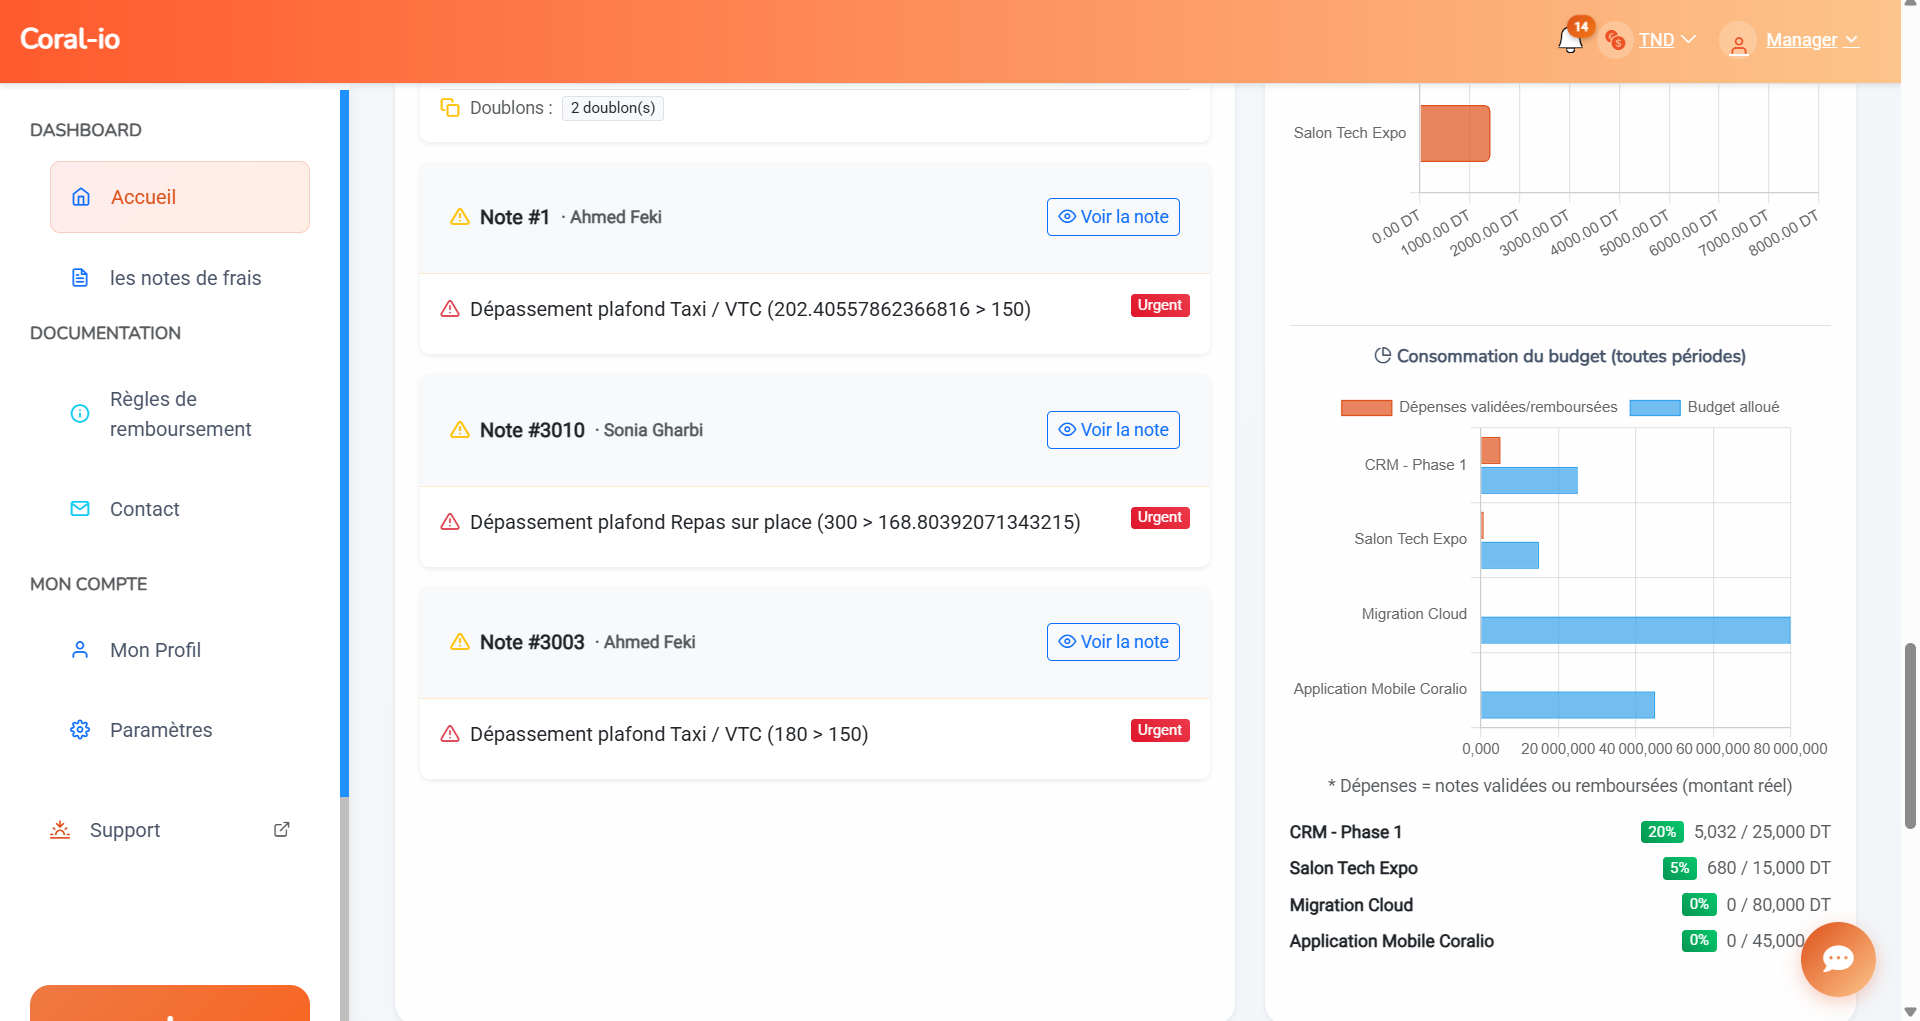
\includegraphics[width=\textwidth]{dashboard-manager/Suite_5.png}

\caption{Suite 4 du tableau de bord manager}

\label{fig:manager_dashboard}

\end{figure}

\begin{figure}[H]

\centering

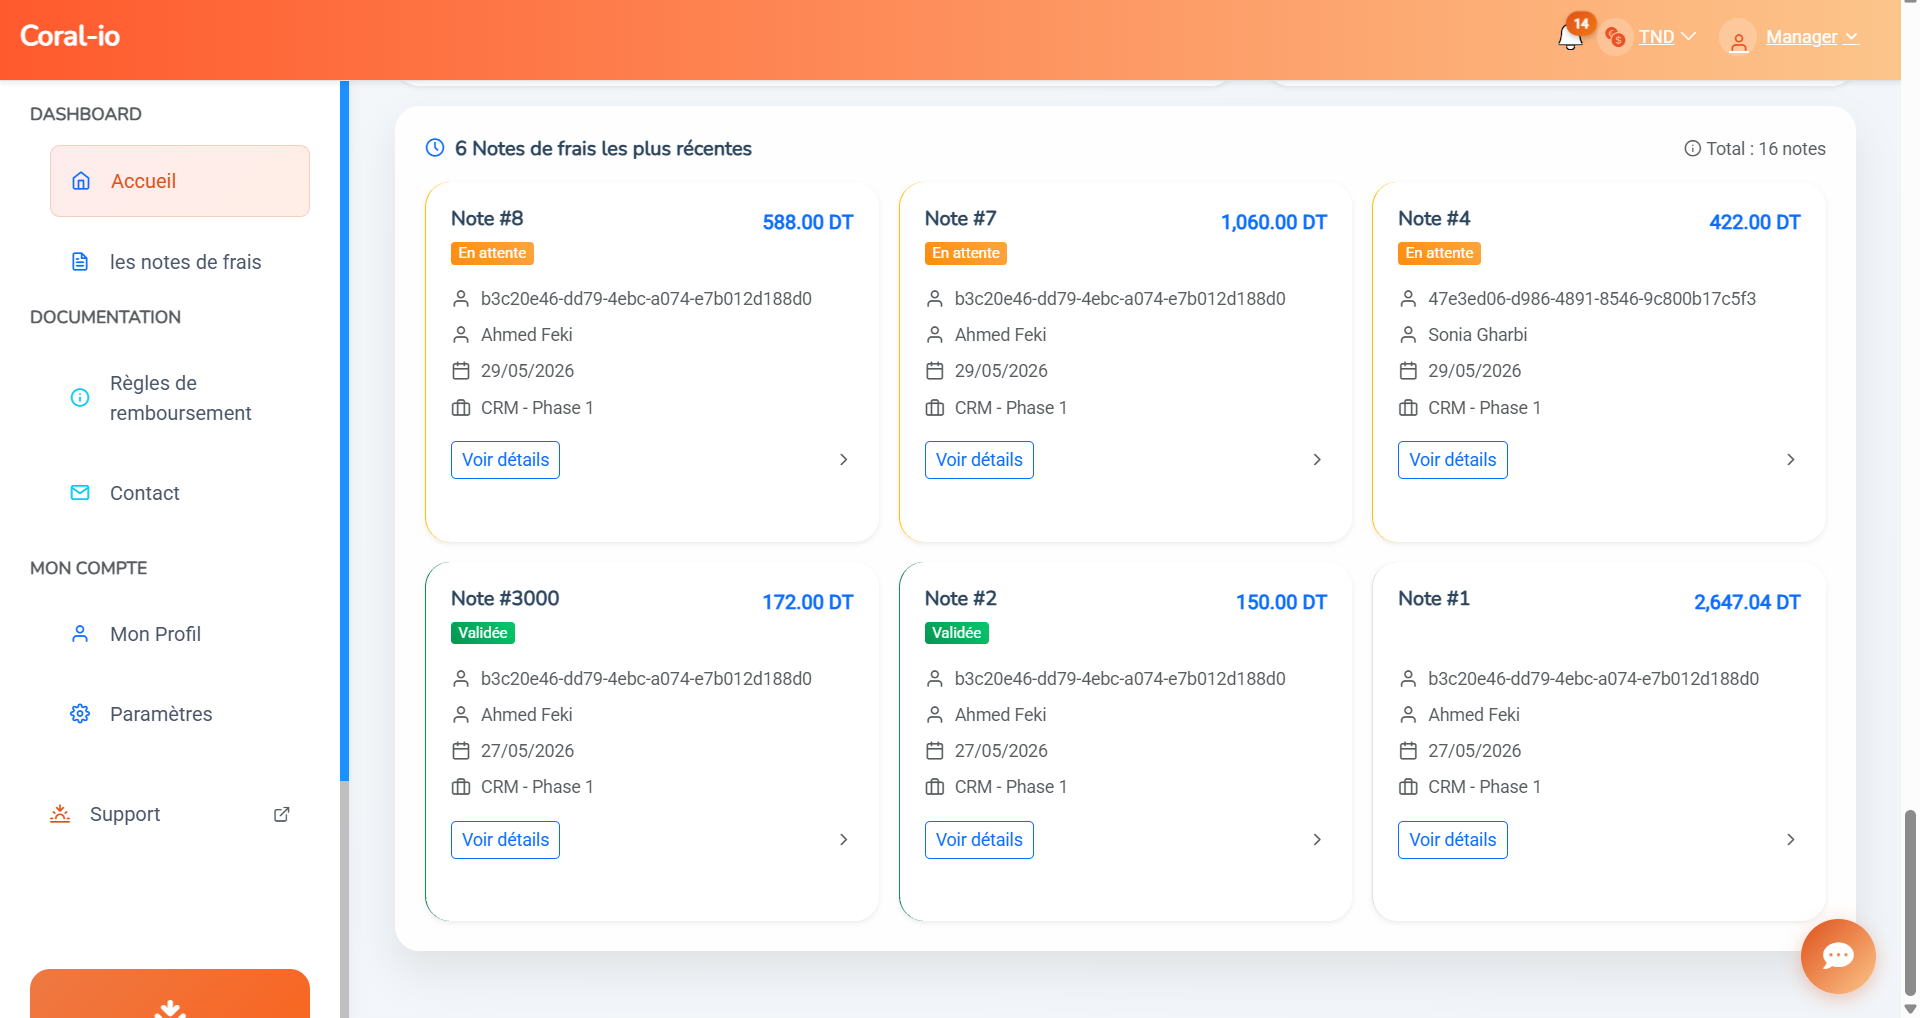
\includegraphics[width=\textwidth]{dashboard-manager/Suite_6.png}

\caption{Suite 5 du tableau de bord manager}

\label{fig:manager_dashboard}

\end{figure}



\subsection{Tableau de bord administrateur}

Le tableau de bord administrateur agrège l'ensemble des indicateurs :

\begin{itemize}

 \item Cartes KPI : notes en attente de validation admin, montant total remboursé, ordres de paiement en attente, taux de validation admin.

 \item Évolution financière (montants soumis vs remboursés par mois).

 \item Top 5 dépensiers (toutes périodes).

 \item Répartition par catégorie (graphique en donut).

 \item Remboursement par département (barres horizontales).

 \item Évolution des fraudes (doublons, dépassements budget, anomalies IA) par mois.

 \item Performance des managers (taux acceptation/refus).

 \item Budget consommé par projet (comparaison budget alloué vs montant remboursé).

 \item Calendrier des remboursements avec les ordres de paiement planifiés.

 \item Audit des actions des managers (paginated).

 \item Exports Excel/CSV.

\end{itemize}



\begin{figure}[H]

\centering

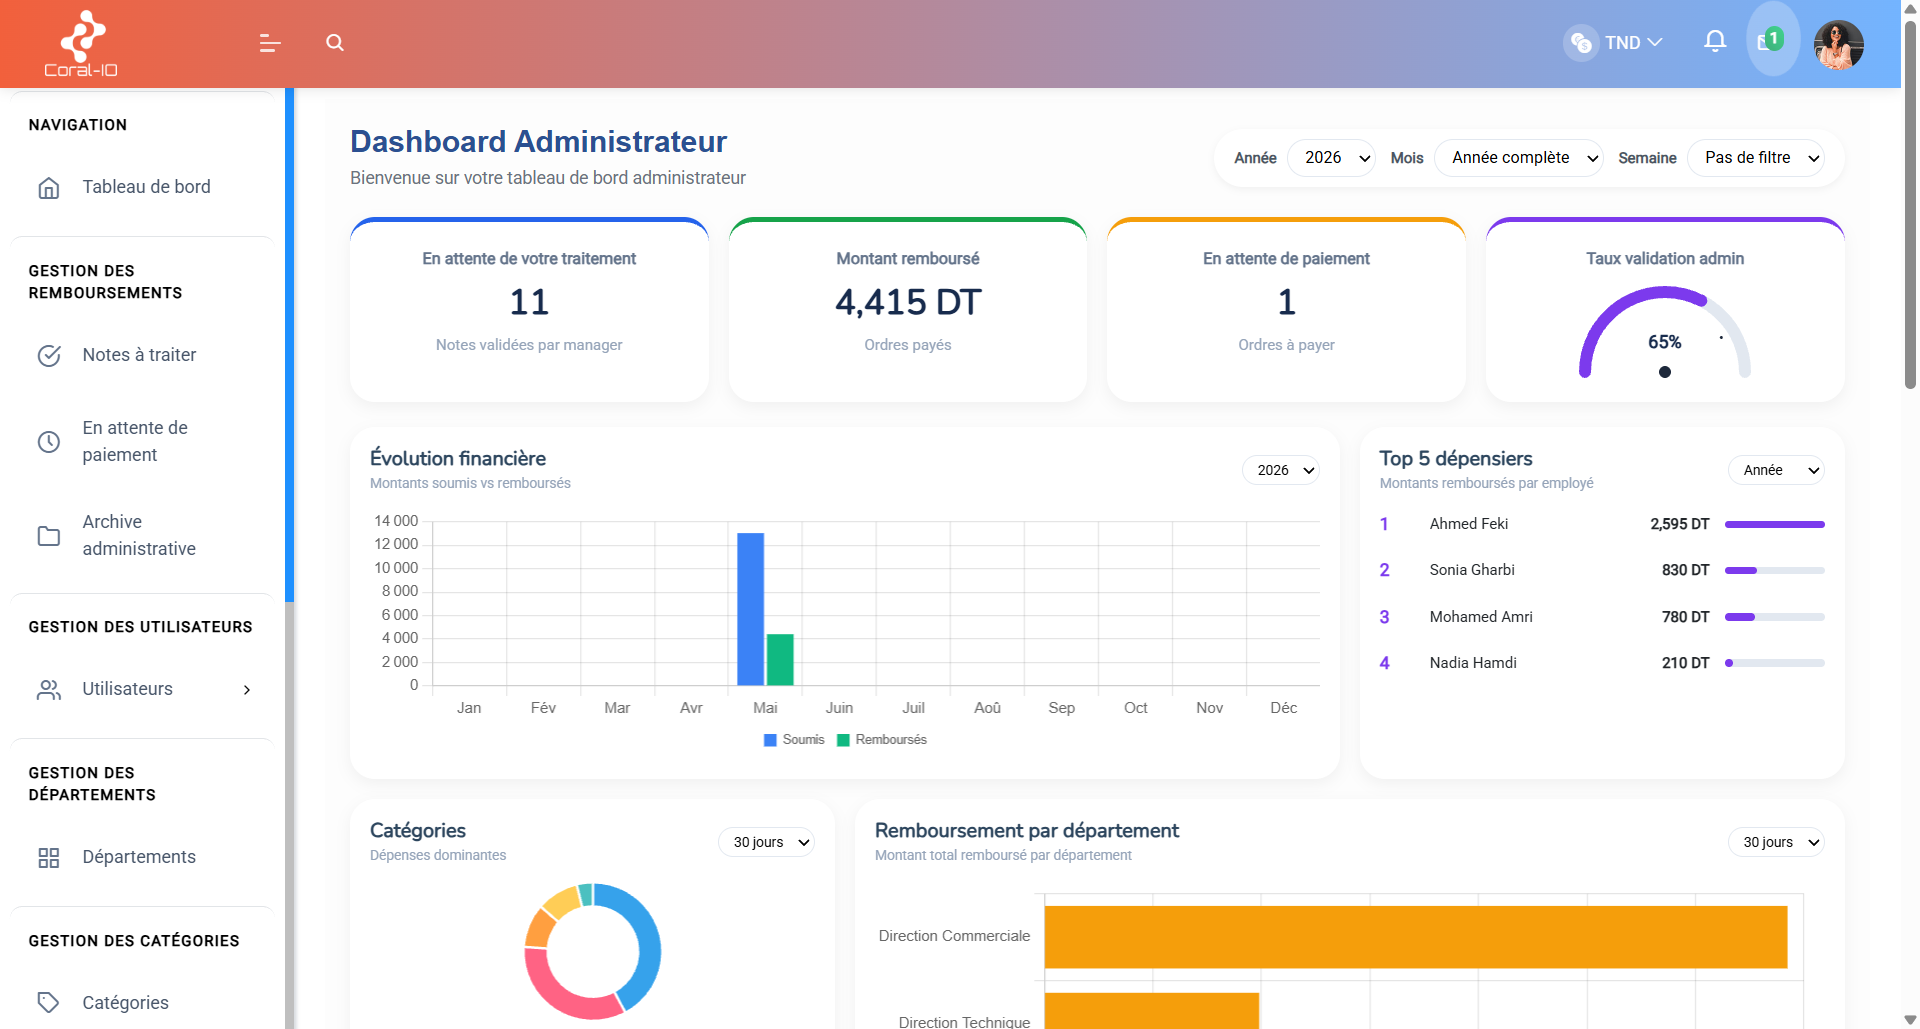
\includegraphics[width=\textwidth]{dashboard-admin/Suite_1.png}

\caption{Tableau de bord administrateur}

\label{fig:admin_dashboard}

\end{figure}

\begin{figure}[H]

\centering

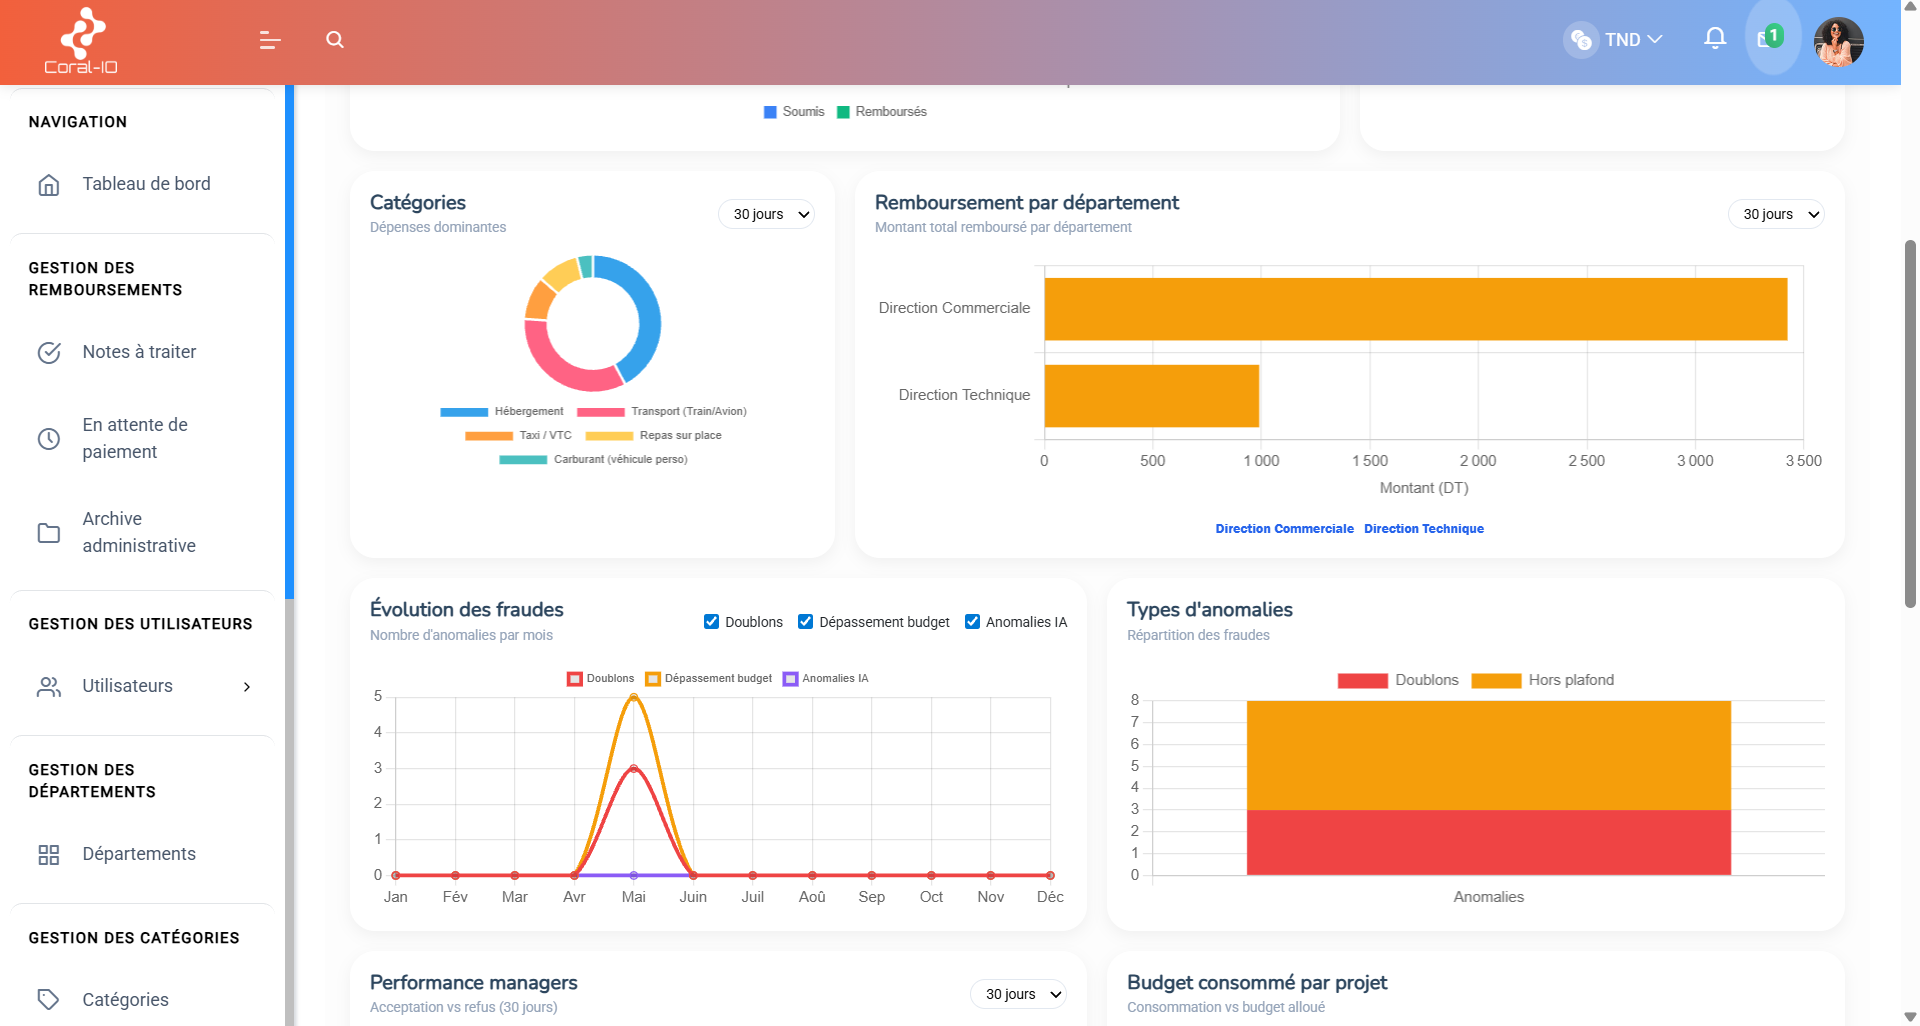
\includegraphics[width=\textwidth]{dashboard-admin/Suite_2.png}

\caption{Suite 1 du tableau de bord administrateur}

\label{fig:admin_dashboard}

\end{figure}

\begin{figure}[H]

\centering

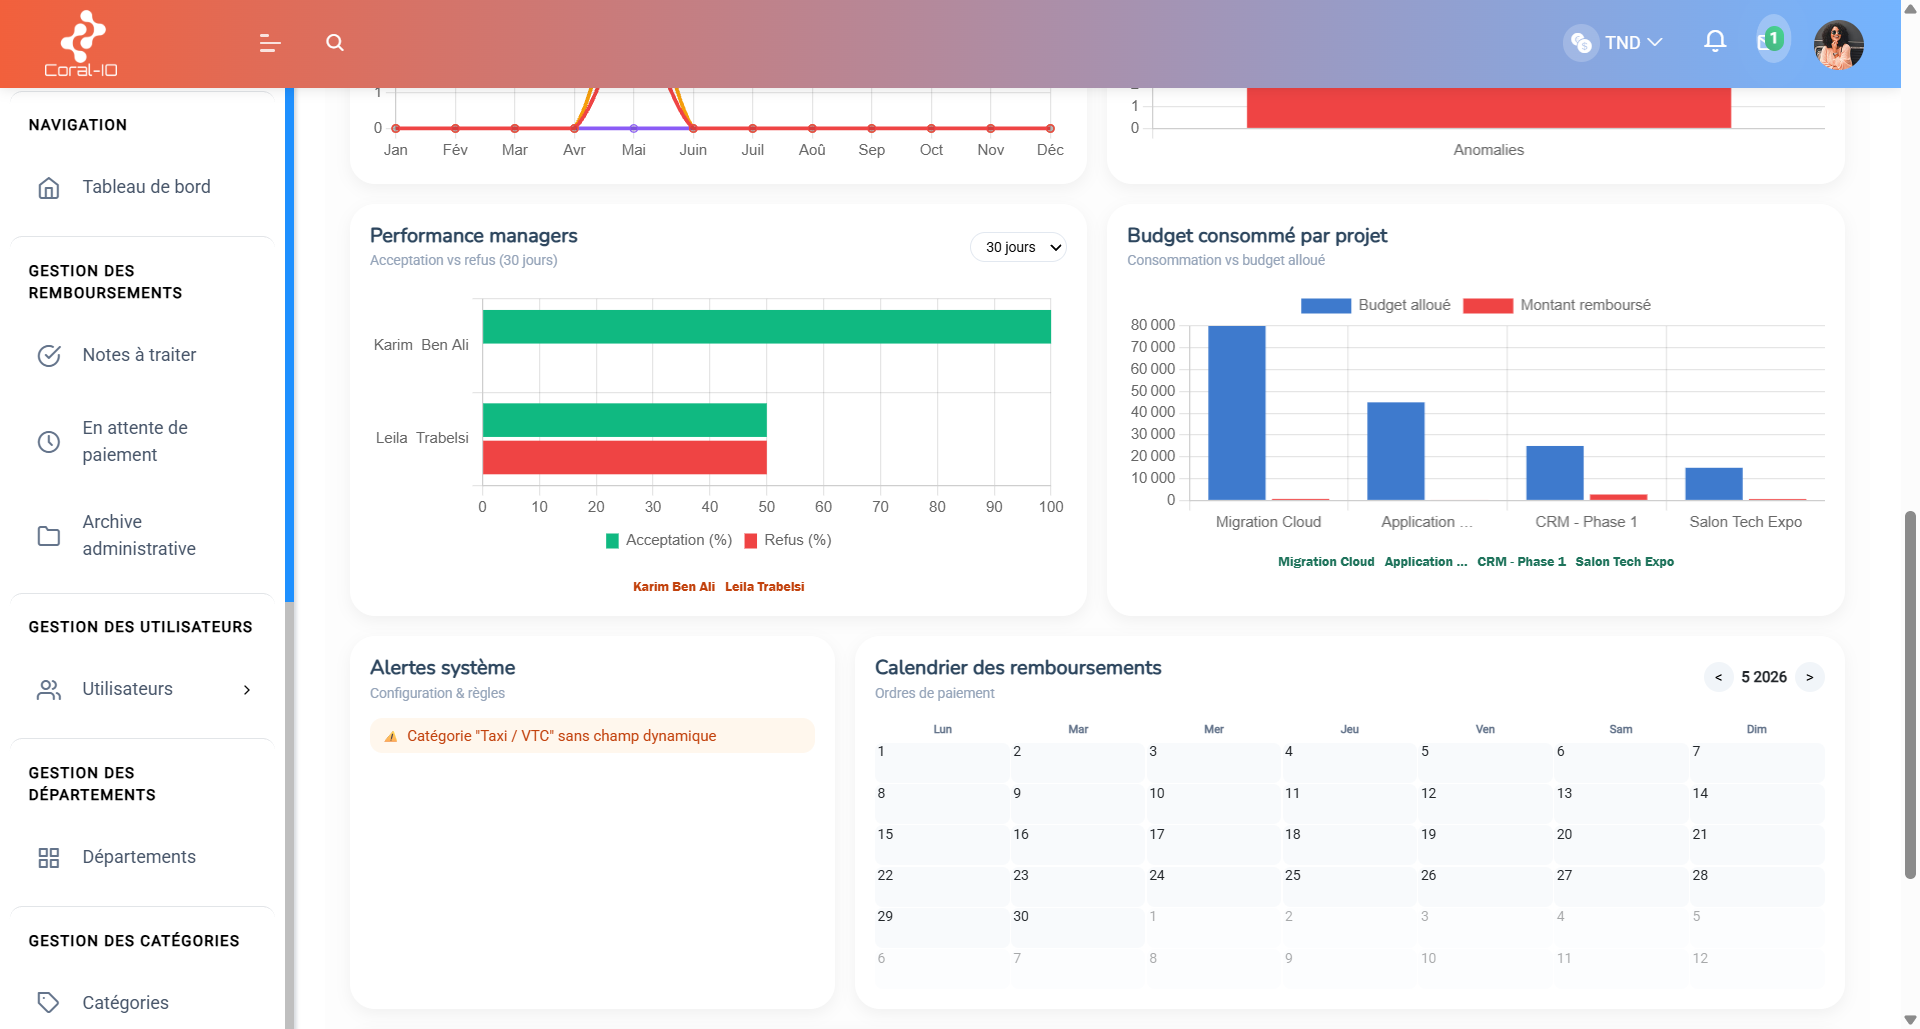
\includegraphics[width=\textwidth]{dashboard-admin/Suite_3.png}

\caption{Suite 2 du tableau de bord administrateur}

\label{fig:admin_dashboard}

\end{figure}

\begin{figure}[H]

\centering

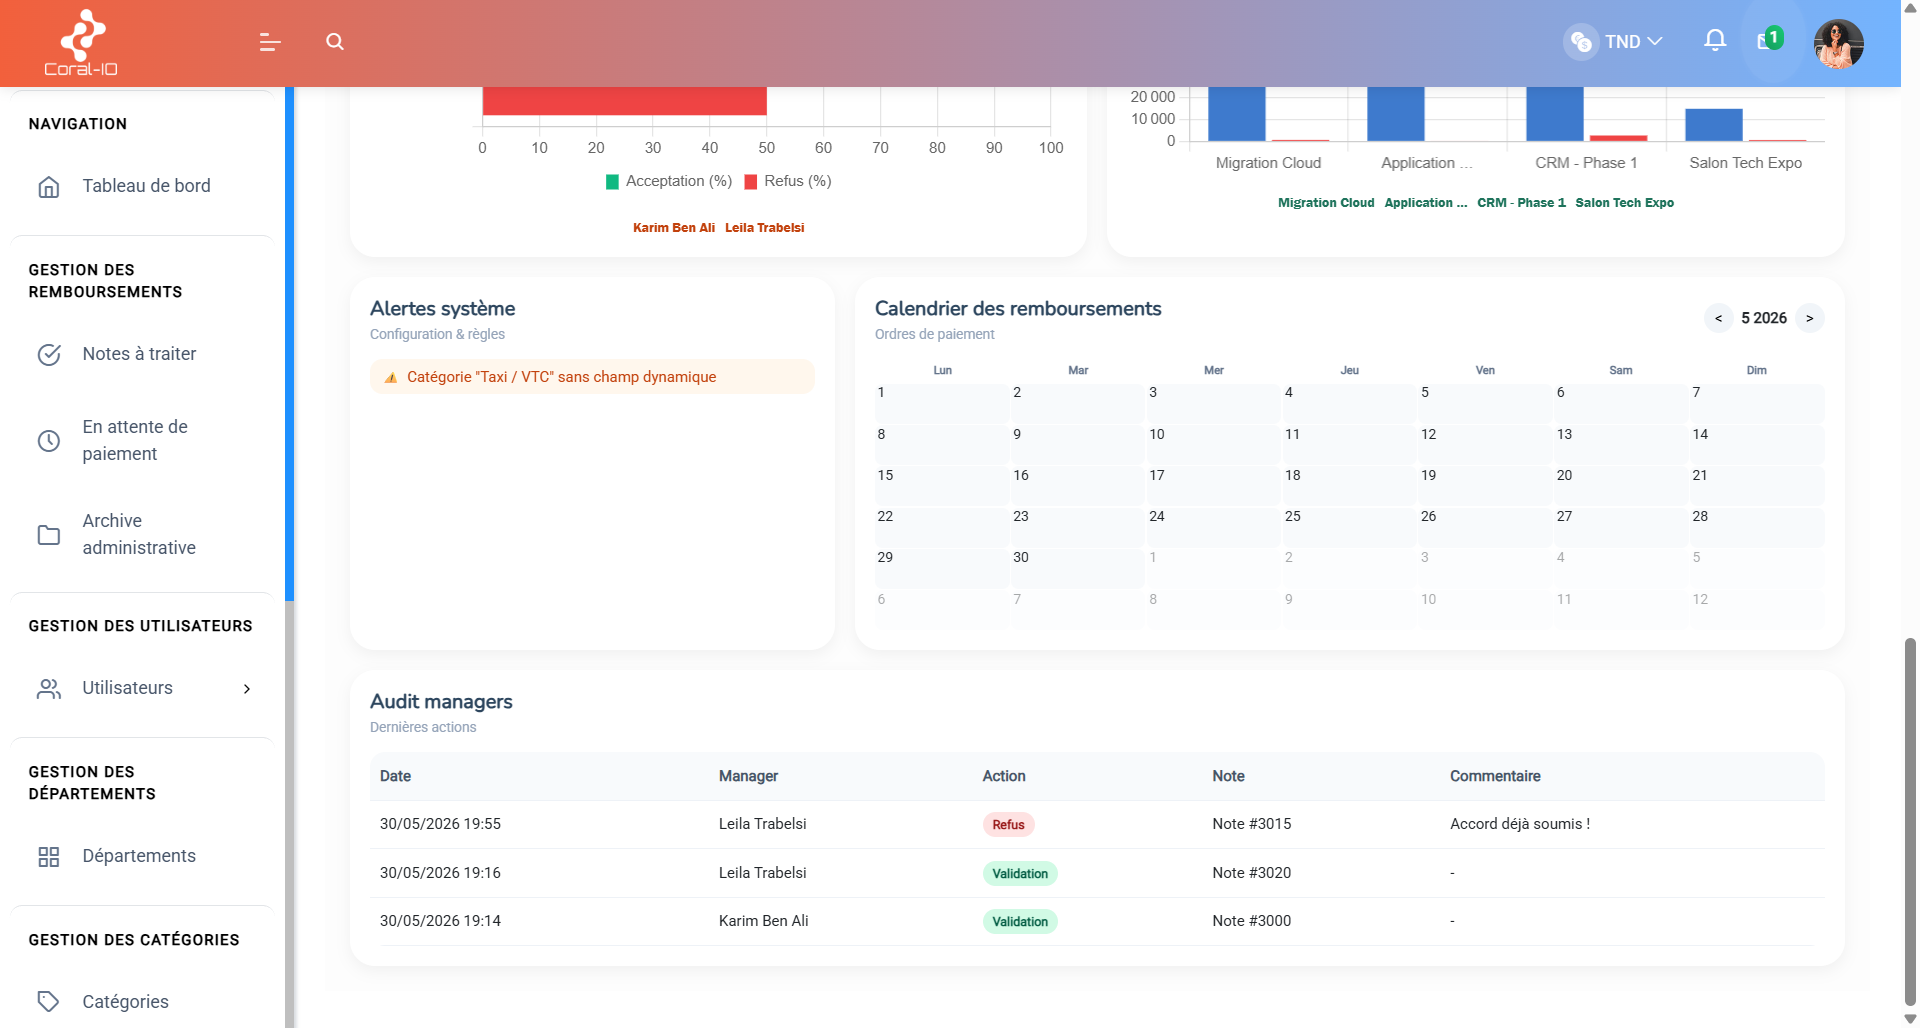
\includegraphics[width=\textwidth]{dashboard-admin/Suite_4.png}

\caption{Suite 3 du tableau de bord administrateur}

\label{fig:admin_dashboard}

\end{figure}



\section{Conclusion}

Grâce à l'application de la méthodologie CRISP-DM, nous avons pu développer et déployer des modèles d'IA performants pour la détection des anomalies dans le processus de notes de frais. L'intégration de FAISS, Isolation Forest et des LLM a permis de couvrir les principaux cas de fraude ou d'erreur. Les tableaux de bord interactifs offrent une vision claire des indicateurs clés et facilitent la prise de décision. Enfin, le chatbot hybride améliore l'expérience utilisateur en apportant une aide instantanée et contextuelle. Ces travaux constituent une base solide pour l'amélioration continue du système.

\chapter*{Conclusion Générale}

\addcontentsline{toc}{chapter}{Conclusion Générale}



En conclusion, le développement de notre application web Coral.io Expense, qui automatise l'ensemble du cycle de vie des notes de frais, de la soumission par l'employé jusqu'au remboursement final, a été une expérience à la fois enrichissante et formatrice.



Ce stage nous a offert une opportunité précieuse de mettre en pratique les compétences techniques acquises tout au long de notre parcours universitaire, tout en renforçant notre sens de responsabilité, notre autonomie et notre aptitude à travailler efficacement en équipe.



L'utilisation de la méthode agile SCRUM nous a permis d'optimiser notre organisation, notre réactivité et la qualité de nos livrables à travers des itérations bien définies.



Le premier sprint nous a permis de poser les fondations essentielles en matière de gestion des comptes utilisateurs, des départements, des projets et des catégories de dépenses, garantissant ainsi une base solide pour une plateforme fonctionnelle et intuitive.



Le deuxième sprint s'est focalisé sur la création et la gestion des notes de frais, incluant la soumission, la modification, la consultation et le processus de validation par le manager, une étape clé pour assurer la fiabilité et la fluidité du workflow.



Le troisième sprint, quant à lui, a introduit la gestion des remboursements, des ordres de paiement ainsi que le déploiement via Docker. Ces éléments renforcent la traçabilité et la sécurité financière de la plateforme.



Enfin, le sprint final a intégré une intelligence artificielle pour la détection automatique des anomalies (doublons, montants suspects, vérification sémantique des justificatifs), un assistant conversationnel hybride, ainsi que des tableaux de bord interactifs adaptés à chaque rôle, offrant ainsi une réelle valeur ajoutée à notre solution.



Nous souhaitons faire évoluer notre application à plus grande échelle en développant une version mobile native, en intégrant des connecteurs comptables avancés, en améliorant les modèles d'IA et en proposant des fonctionnalités d'analytique prédictive, afin de construire une solution complète où toute entreprise soucieuse de maîtriser ses coûts puisse facilement trouver une réponse adaptée à ses besoins.


% ============================================================
% WEBLIOGRAPHIE
% ============================================================

\begin{thebibliography}{99}

% ============================================================
% CONTEXTE PROJET & ENTREPRISE
% ============================================================

\bibitem{coralio} Coral-io, \textit{Solution de gestion des notes de frais Coral.io Expense}, [En ligne], Disponible : \url{https://coral-io.com/}, (Consulté le 10/02/2025).


% ============================================================
% SOLUTIONS CONCURRENTES (ÉTUDE DE L'EXISTANT)
% ============================================================

\bibitem{sapconcur} SAP Concur, \textit{Gestion des notes de frais et dépenses professionnelles}, [En ligne], Disponible : \url{https://www.concur.com/}, (Consulté le 15/02/2025).

\bibitem{expensya} Expensya, \textit{Application de gestion des notes de frais}, [En ligne], Disponible : \url{https://www.expensya.com/}, (Consulté le 15/02/2025).

\bibitem{rydoo} Rydoo, \textit{Solution de gestion des notes de frais}, [En ligne], Disponible : \url{https://www.rydoo.com/}, (Consulté le 15/02/2025).


% ============================================================
% MÉTHODOLOGIES DE GESTION DE PROJET
% ============================================================

\bibitem{scrum} Scrum.org, \textit{The Scrum Guide - Guide officiel de la méthodologie Scrum}, [En ligne], Disponible : \url{https://scrumguides.org/}, (Consulté le 25/02/2025).

\bibitem{crispdm} The Modeling Agency, \textit{CRISP-DM - Cross-Industry Standard Process for Data Mining}, [En ligne], Disponible : \url{https://www.the-modeling-agency.com/crisp-dm.pdf}, (Consulté le 25/05/2025).

\bibitem{kdd} KDnuggets, \textit{Knowledge Discovery in Databases (KDD) Process}, [En ligne], Disponible : \url{https://www.kdnuggets.com/gps.html}, (Consulté le 25/05/2025).

\bibitem{semma} SAS Institute, \textit{SEMMA: SAS Data Mining Methodology}, [En ligne], Disponible : \url{https://www.sas.com/}, (Consulté le 25/05/2025).


% ============================================================
% INTELLIGENCE ARTIFICIELLE & MACHINE LEARNING
% ============================================================

\bibitem{ollama} Ollama, \textit{Exécuter des LLM en local - Documentation officielle}, [En ligne], Disponible : \url{https://ollama.com/}, (Consulté le 20/05/2025).

\bibitem{gemma} Google AI, \textit{Gemma - Modèle de langage open source}, [En ligne], Disponible : \url{https://ai.google.dev/gemma}, (Consulté le 20/05/2025).

\bibitem{mistral} Mistral AI, \textit{Mistral 7B - Modèle de langage}, [En ligne], Disponible : \url{https://mistral.ai/news/announcing-mistral-7b/}, (Consulté le 20/05/2025).

\bibitem{llama} Meta AI, \textit{Llama 3 - Modèle de langage}, [En ligne], Disponible : \url{https://llama.meta.com/}, (Consulté le 20/05/2025).

\bibitem{faiss} Facebook Research, \textit{FAISS - Bibliothèque de recherche de similarité vectorielle}, [En ligne], Disponible : \url{https://github.com/facebookresearch/faiss}, (Consulté le 15/05/2025).

\bibitem{sentencebert} Hugging Face, \textit{Sentence Transformers - Documentation officielle}, [En ligne], Disponible : \url{https://www.sbert.net/}, (Consulté le 15/05/2025).

\bibitem{minilm} Hugging Face, \textit{all-MiniLM-L6-v2 - Modèle d'embedding}, [En ligne], Disponible : \url{https://huggingface.co/sentence-transformers/all-MiniLM-L6-v2}, (Consulté le 15/05/2025).

\bibitem{bert} Google Research, \textit{BERT - Modèle de langage}, [En ligne], Disponible : \url{https://github.com/google-research/bert}, (Consulté le 15/05/2025).

\bibitem{camembert} Hugging Face, \textit{CamemBERT - Modèle de langue français}, [En ligne], Disponible : \url{https://huggingface.co/camembert-base}, (Consulté le 15/05/2025).

\bibitem{isolationforest} Scikit-learn, \textit{Isolation Forest - Détection d'anomalies}, [En ligne], Disponible : \url{https://scikit-learn.org/stable/modules/generated/sklearn.ensemble.IsolationForest.html}, (Consulté le 15/05/2025).

\bibitem{scikitlearn} Scikit-learn, \textit{Scikit-learn - Bibliothèque Machine Learning pour Python}, [En ligne], Disponible : \url{https://scikit-learn.org/}, (Consulté le 15/05/2025).

\bibitem{pandas} Pandas, \textit{Pandas - Bibliothèque d'analyse de données pour Python}, [En ligne], Disponible : \url{https://pandas.pydata.org/}, (Consulté le 15/05/2025).


% ============================================================
% OCR (RECONNAISSANCE OPTIQUE DE CARACTÈRES)
% ============================================================

\bibitem{paddleocr} PaddlePaddle, \textit{PaddleOCR - Reconnaissance optique de caractères}, [En ligne], Disponible : \url{https://github.com/PaddlePaddle/PaddleOCR}, (Consulté le 15/05/2025).

\bibitem{tesseract} Google, \textit{Tesseract OCR - Moteur de reconnaissance de caractères}, [En ligne], Disponible : \url{https://github.com/tesseract-ocr/tesseract}, (Consulté le 15/05/2025).

\bibitem{pdfplumber} KnowledgeTeam, \textit{pdfplumber - Extraction de texte depuis PDF}, [En ligne], Disponible : \url{https://github.com/jsvine/pdfplumber}, (Consulté le 15/05/2025).

\bibitem{rapidfuzz} Bachmann, M., \textit{RapidFuzz - Recherche floue en Python}, [En ligne], Disponible : \url{https://github.com/rapidfuzz/RapidFuzz}, (Consulté le 20/05/2025).


% ============================================================
% FRAMEWORKS BACK-END & MICROSERVICES
% ============================================================

\bibitem{spring} VMware, \textit{Spring Boot - Framework Java pour microservices}, [En ligne], Disponible : \url{https://spring.io/projects/spring-boot}, (Consulté le 20/02/2025).

\bibitem{fastapi} FastAPI, \textit{FastAPI - Framework Python pour APIs}, [En ligne], Disponible : \url{https://fastapi.tiangolo.com/}, (Consulté le 25/02/2025).

\bibitem{keycloak} Keycloak, \textit{Keycloak - Authentification et gestion des rôles}, [En ligne], Disponible : \url{https://www.keycloak.org/}, (Consulté le 25/02/2025).


% ============================================================
% LANGAGES DE PROGRAMMATION
% ============================================================

\bibitem{java} Oracle, \textit{Java - Langage de programmation}, [En ligne], Disponible : \url{https://www.java.com/}, (Consulté le 20/02/2025).


% ============================================================
% FRAMEWORKS FRONT-END
% ============================================================

\bibitem{angular} Google, \textit{Angular - Framework pour applications web}, [En ligne], Disponible : \url{https://angular.io/}, (Consulté le 25/02/2025).

\bibitem{typescript} Microsoft, \textit{TypeScript - Langage typé pour JavaScript}, [En ligne], Disponible : \url{https://www.typescriptlang.org/}, (Consulté le 25/02/2025).

\bibitem{bootstrap} Bootstrap, \textit{Bootstrap - Bibliothèque CSS responsive}, [En ligne], Disponible : \url{https://getbootstrap.com/}, (Consulté le 25/02/2025).

\bibitem{scss} Sass, \textit{SCSS - Extension CSS}, [En ligne], Disponible : \url{https://sass-lang.com/}, (Consulté le 25/02/2025).


% ============================================================
% BASE DE DONNÉES
% ============================================================

\bibitem{postgresql} PostgreSQL, \textit{PostgreSQL - Base de données relationnelle}, [En ligne], Disponible : \url{https://www.postgresql.org/docs/}, (Consulté le 16/03/2025).


% ============================================================
% CONTENEURISATION & DÉPLOIEMENT
% ============================================================

\bibitem{docker} Docker, \textit{Docker - Plateforme de conteneurisation}, [En ligne], Disponible : \url{https://www.docker.com/}, (Consulté le 14/04/2025).


% ============================================================
% VERSIONNEMENT & COLLABORATION
% ============================================================

\bibitem{git} Git, \textit{Git - Outil de versionnement}, [En ligne], Disponible : \url{https://git-scm.com/}, (Consulté le 20/02/2025).

\bibitem{github} GitHub, \textit{GitHub - Plateforme d'hébergement de code}, [En ligne], Disponible : \url{https://github.com/}, (Consulté le 14/04/2025).


% ============================================================
% DESIGN, MAQUETTAGE & TESTS
% ============================================================

\bibitem{drawio} diagrams.net, \textit{draw.io - Outil de conception de diagrammes}, [En ligne], Disponible : \url{https://www.diagrams.net/}, (Consulté le 20/02/2025).

\bibitem{figma} Figma, \textit{Figma - Outil de conception d'interfaces}, [En ligne], Disponible : \url{https://www.figma.com/}, (Consulté le 20/02/2025).

\bibitem{postman} Postman, \textit{Postman - Test et documentation d'API REST}, [En ligne], Disponible : \url{https://www.postman.com/}, (Consulté le 25/02/2025).


% ============================================================
% ENVIRONNEMENTS DE DÉVELOPPEMENT (IDE)
% ============================================================

\bibitem{vscode} Microsoft, \textit{Visual Studio Code - Éditeur de code}, [En ligne], Disponible : \url{https://code.visualstudio.com/}, (Consulté le 20/02/2025).

\bibitem{intellij} JetBrains, \textit{IntelliJ IDEA - IDE pour Java}, [En ligne], Disponible : \url{https://www.jetbrains.com/idea/}, (Consulté le 20/02/2025).

\bibitem{pycharm} JetBrains, \textit{PyCharm - IDE pour Python}, [En ligne], Disponible : \url{https://www.jetbrains.com/pycharm/}, (Consulté le 20/02/2025).


% ============================================================
% UML (LANGAGE DE MODÉLISATION)
% ============================================================

\bibitem{uml} OMG, \textit{UML - Unified Modeling Language}, [En ligne], Disponible : \url{https://www.uml.org/}, (Consulté le 20/02/2025).

\end{thebibliography}
\clearpage

\thispagestyle{empty}

\vspace*{2cm}

\begin{center}

 {\Huge \bfseries Résumé}

\end{center}

\vspace{0.5cm}



Ce travail s'inscrit dans le cadre du projet de fin d'études réalisé au sein de l'entreprise Coral-io. L'objectif de ce projet est la conception et le développement d'une application web dédiée à la gestion des notes de frais, nommée Coral.io Expense. Cette solution vise à répondre aux besoins croissants des entreprises tunisiennes en matière d'optimisation des processus financiers et de maîtrise des coûts. Le projet a permis la mise en œuvre d'une plateforme numérique automatisant l'ensemble du cycle de vie des notes de frais, de la soumission par l'employé jusqu'au remboursement final, en passant par un workflow de validation structuré à trois niveaux (Manager, Administrateur, Remboursement), une détection intelligente des anomalies basée sur l'intelligence artificielle, une gestion multi-devises en temps réel, ainsi que des tableaux de bord interactifs adaptés à chaque rôle.



\textbf{Mots clés :} Angular, Spring Boot, Python, FastAPI, PostgreSQL, Keycloak, Docker, Intelligence Artificielle, OCR, LLM, FAISS, Détection d'anomalies, Notes de frais



\vspace{1cm}



\begin{center}

 {\Huge \bfseries Abstract}

\end{center}

\vspace{0.5cm}



\begin{otherlanguage}{english}

This work is part of the final-year project carried out with the company Coral-io. The objective of this project is the design and development of a web application dedicated to expense report management, named Coral.io Expense. This solution aims to meet the growing needs of Tunisian companies in terms of financial process optimization and cost control. The project enabled the implementation of a digital platform that automates the entire expense report lifecycle, from submission by the employee to final reimbursement, through a structured three-level validation workflow (Manager, Administrator, Reimbursement), intelligent anomaly detection based on artificial intelligence, real-time multi-currency management, as well as interactive dashboards adapted to each role.



\textbf{Keywords:} Angular, Spring Boot, Python, FastAPI, PostgreSQL, Keycloak, Docker, Artificial Intelligence, OCR, LLM, FAISS, Anomaly Detection, Expense Reports

\end{otherlanguage}



\end{document}